\documentclass[a4paper,12pt]{report}
\usepackage{lgrind}
\pagestyle{plain}
\usepackage{amsmath,amsfonts,amssymb,amsthm}
\usepackage{listings}
\usepackage{cancel}
\usepackage{appendix}
\usepackage{fancyhdr}   
\usepackage{url}
\usepackage{path}
\usepackage[dvipdfm]{graphicx}
\usepackage{color}
\usepackage{array}
\usepackage{authblk}
\usepackage[margin=2cm, head=2cm, foot=1cm]{geometry}
\usepackage{verbatim}
\setlength{\topmargin}{-2.5cm}
\setlength{\textwidth}{17cm}
\setlength{\oddsidemargin}{-0.5cm}
\setlength{\evensidemargin}{-0.5cm}
\setlength{\textheight}{22.5cm}
\setlength{\footskip}{1cm}
\renewcommand{\topfraction}{0.9}
\renewcommand{\bottomfraction}{0.8}
\setcounter{topnumber}{2}
\setcounter{bottomnumber}{2}
\setcounter{totalnumber}{4}
\usepackage{hyperref}
\usepackage{pdfpages}
\lstset{columns=fullflexible,basicstyle=\ttfamily}



\newcommand{\ROOT}{{\ttfamily ROOT} }
\newcommand{\CINT}{{\ttfamily CINT} }
\newcommand{\CPP}{{\ttfamily C++} }
\newcommand{\gpp}{{\ttfamily g++} }
\newcommand{\clang}{{\ttfamily clang} }
\newcommand{\python}{{\ttfamily python} }
\newcommand{\PyROOT}{{\ttfamily PyROOT} }
\newcommand{\larsoft}{{\ttfamily LArSoft} }
\newcommand{\git}{{\ttfamily git} }
\newcommand{\doxygen}{{\ttfamily doxygen} }
\newcommand{\Base}{{\ttfamily Base} }
\newcommand{\Core}{{\ttfamily core} }
\newcommand{\DataFormat}{{\ttfamily DataFormat} }
\newcommand{\Analysis}{{\ttfamily Analysis} }
\newcommand{\anaunit}{{\ttfamily AnalysisUnit} }
\newcommand{\anaproc}{{\ttfamily AnaProcessor} }
\newcommand{\LArUtil}{{\ttfamily LArUtil} }
\newcommand{\UserDev}{{\ttfamily UserDev} }
\newcommand{\Geometry}{{\ttfamily Geometry} }
\newcommand{\GeometryUtilities}{{\ttfamily GeometryUtilities} }
\newcommand{\LArProperties}{{\ttfamily LArProperties} }
\newcommand{\DetectorProperties}{{\ttfamily DetectorProperties} }
\newcommand{\HTML}{{\ttfamily HTML} }
\newcommand{\FEMPulseReco}{{\ttfamily FEMPulseReco} }
\newcommand{\FEMPulseStudy}{{\ttfamily FEMPulseStudy} }
\newcommand{\ART}{{\ttfamily ART} }
\newcommand{\ertool}{{\ttfamily ERTool} }
\newcommand{\enum}{{\ttfamily enum} }
\newcommand{\LiteScanner}{{\ttfamily LiteScanner} }
\newcommand{\tuple}{{\ttfamily TNtuple}}


\begin{document}

\title{LArLight \\ \vspace{0.1in} Simple LArSoft Data Analysis Tool}
\date{March 12th, 2014}
\author{Kazuhiro Terao, kazuhiro@nevis.columbia.edu}
\maketitle

\begin{abstract}
LArLight is a simple \CPP + \ROOT analysis framework for LArSoft data. The goal of the framework is to provide (1) a generic \CPP \& \ROOT code development environment with build support on various platform, (2) an access to {\it ala} LArSoft data and utiltiy classes outside LArSoft framework, and (3) analysis framework for data processing. It fits somewhere between LArSoft and {\ttfamily AnalysisTree}. It is suitable for those who want to access details of LArSoft data and develop analysis/reconstruction code quickly. One of LArLight design principles is to be flexible and comfortable to developers. The framework builds on multiple platforms (Linux and OSX Darwin) and supports various ways to execute the compiled code (compiled executable or \CINT/\PyROOT interpreter scripts). It comes with a simple package generator that include a build system. It can be also used just as a \CPP play ground for students. Please feel free to use it for any purpose. The author is happy to be contacted for questions/suggestions anytime.
\end{abstract}

% Table of Contents
\tableofcontents

\newpage
% How-to on setting things up
\chapter{Installation}
\label{chap:installation}

This chapter discuss about how to generating user's own code development space.
In particular following itmes are discussed in the respective order.
\begin{itemize}
\item Getting started: your own code repository
\item A simple \CPP project package 
\item Stuffing your package
\begin{itemize}
  \item Simple \CPP class
  \item \anaunit (see Ch.\ref{chap:analysis}).
  \item \ertool algorithm class (see \ertool documentation)
  \item \ertool filter class (see \ertool documentation)
  \item \ertool analysis class (see \ertool documentation)
  \item \CPP functions
\end{itemize}
\item Details: LArLite build basics
\item Advanced Code Development
\begin{itemize}
  \item \CPP functions outside classes
  \item Inter-package dependence
  \item Data product: storing \CPP class instance in \ROOT file
  \item \python in \CPP (i.e. opposite of \PyROOT)
\end{itemize}
\end{itemize}

\section{Creating Your Repository}
\label{sec:devrepo}

LArLite supports user code development under \UserDev.
More precisely, it is assumed to be under any path that is set to the value of shell environment variable {\ttfamily \$LARLITE\_USERDEVDIR}. 
For the sake of simplicity we stick with \UserDev in this section.

\subsection{Note About \UserDev}
Important note first:
\begin{itemize}
  \item {\ttfamily UserDev/GNUmakefile}, if it exists, is generated by setup.sh and it does not belong to LArLite repository (ignore it).
  \item Some sub-directories belong to LArLite (see below). Some of these depend on LArLite and some don't. It is useful to note them briefly here.
    \begin{itemize}
        \item {\ttfamily BasicTool} contains useful packages like {\ttfamily GeoAlgo} and has no dependency outside
        \item {\ttfamily SelectionTool} contains useful packages like {\ttfamily ERTool} and depends on {\ttfamily BasicTool}
        \item {\ttfamily RecoTool} contains shower reconstruction code and depends on {\ttfamily core}
        \item {\ttfamily LArLiteApp} contains LArLite application from {\ttfamily GeoAlgo} and {\ttfamily ERTool} 
    \end{itemize}
  \item You can create new directories under \UserDev and that won't bother other users. We'll do this below. 
  This is all done through {\ttfamily .gitignore} rule placed under the top directory. 
\end{itemize}

These features of \UserDev are there so that you feel more free to make a mess (sorry, I meant, to develop code) there!

\subsection{Creating Your Sub-Repository in \UserDev}
\label{sec:devrepo:makenew}
Obviously I cannot just say ``do whatever under \UserDev'' and leave: I would love to support a very easy way to develop code (or make a mess) under \UserDev. I will just show you how to do things here:
\begin{lstlisting}
     > llgen_repository MyRepo
\end{lstlisting}
where the execution command is an alias explained in Sec.\ref{sec:configure}.
This should create a new directory called {\ttfamily MyRepo} under \UserDev. 
That is your new repository. As said, this does not affect LArLite repository. 
If you don't want to keep {\ttfamily MyRepo}, simply ``{\ttfamily rm -r}'' it.

Another thing to note here: your repository will contain code and you will compile them, making a compiled shared object library. 
Your repository name will be used to name your library file (if you follow LArLite code generation scripts described in the followings). 
So pick a name that suits for your purpose. You do not want to pick a generic name that might coincide with some other libraries on your machine.

\subsection{What's in MyRepo?}

Your new repository comes with a GNUmakefile (which does nothing for now) and {\ttfamily doc} 
directory with a doxygen script but empty otherwise. Under this space, you can create your ``packages'' as a 
set of \CPP code to be compiled into a library. We will discuss about more later.

\subsection{Creating Your Sub-Repository in {\ttfamily github}}
In the previous section, we created a new repository {\ttfamily MyRepo} under \UserDev. But that's just a directory on your laptop, and you may want to keep it as your code repository using either {\ttfamily svn} or {\ttfamily github} (or anything else you would like to use). Here, I briefly mention how you can do this using {\ttfamily github} because it's very easy given that you already have a {\ttfamily github} account.

First of all, go to {\ttfamily github.com} and create your own repository: go to your {\ttfamily github} account web page, and click on ``+'' symbol that is toward right-top of the web page. Choose ``New repository''. Then enter the repository name you are about to create. Ideally you may want to choose a somewhat unique name as described in Sec.\ref{sec:devrepo:makenew}. You can always remove your repository if you don't like it.

Then checkout your empty repository. As an example, I use my empty repo called {\ttfamily EmptyRepo}.
\begin{lstlisting}
    > cd $LARLITE_USERDEVDIR
    > git clone git@github.com:drinkingkazu/EmptyRepo EmptyRepo
\end{lstlisting}
Now simply run:
\begin{lstlisting}
    > python bin/gen_new_repository EmptyRepo
    > cd EmptyRepo
    > git add .
    > git commit -m ``new repository''
    > gitpush -u origin master
\end{lstlisting}
and you are done!
From the next time, if you want to install LArLite from scratch, simply checkout your repository under UserDev with the same name.

As said many times, of course, your repository is independent of LArLite repository.





\section{Creating a Package}
\label{sec:package}
Here, I assume we are working under {\ttfamily UserDev/MyRepo}. 
In fact, since it's tedious, I will just refer to {\ttfamily MyRepo}.

\subsection{What is a ``Package''?}
``Package'' is a directory under a repository that is compiled and generates one {\bf shred object library}
(i.e. a file with {\ttfamily .so} extension). This library is loaded at a run-time or linked via compiler as one byte code file.
This gives you a sense of what to include in one package: having too many classes (and especially unrelated classes) in one package
means an extra overhead cost for a run-time loading or linking at compilation. In other words, you probably do not want make one 
library per class, but also not one library for all classes. A package should contain a group of \CPP classes/functions which you
think it makes sense to put together.

\subsection{Making a Simple \CPP Package}

Like advertised many times, LArLite was originally a \CPP project play ground for summer students. 
The author thinks it's very important to have an empty \CPP package generator that comes with build system, 
so that a user can focus on writing the algorithm instead of figuring out how to compile and such.

So here it is: there is a \python script to generate an empty \CPP package:
\begin{lstlisting}
    $LARLITE_BASEDIR/bin/gen_package
\end{lstlisting}
This script takes one input argument which is used to name a ``package'', a directory to be created under {\ttfamily MyRepo}.
This script {\bf needs to be executed somewhere under {\ttfamily MyRepo}} (otherwise you'll see an error message).
One can run this script via alias:
\begin{lstlisting}
    > llgen_package MyProject
\end{lstlisting}
which will create a directory {\ttfamily MyRepo/MyProject} that include minimal set of source codes to compile an empty \CPP class. 
You can have your name choice in place of ``MyProject''. After running the command, try:
\begin{lstlisting}
    > cd MyProject
    > make -j4
\end{lstlisting}
This compiles your code and makes {\ttfamily libMyRepo\_MyProject.so} under {\ttfamily lib} directory.
What you compiled is a \CPP class called ``sample'' defined in {\ttfamily sample.h}. 


\subsection{Using in Interpreter}

So how can you ``use'' this \CPP class? You can write a binary executable code, or try out in \CINT or \PyROOT. Here is an example:
\begin{lstlisting}
    > root
    root[0] sample k;
\end{lstlisting}
Above lines work (i.e. your class instance is created) because \CINT is informed about your class. 

\subsection{``Hello World'' Development}
\label{sec:helloworld}
Let's try a simple modification to your class. Here's an example ``hello world'' program using \CPP class. Open {\ttfamily sample.h} and add a {\ttfamily void} function as shown below:
\begin{lstlisting}
class sample{
public:
  /// Default constructor
  sample(){};
  /// Default destructor
  virtual ~sample(){};
  /// Hello world!
  void HelloWorld() { std::cout << ``Hello World!'' << std::endl; }
};
\end{lstlisting}
Save, close and compile (i.e. type ``make''). Now, try the following in \CINT or \PyROOT:
\begin{lstlisting}
    > root
    root[0] sample k;
    root[1] k.HelloWorld();
    Hello World!
    root[2]
\end{lstlisting}

Whenever you want to start a new project with an empty class, you can come back to this example and create your new \CPP project!





\section{Adding Basic \CPP Classes}
\label{sec:expand_package}

As discussed in the previous section, one should populate a package with a group of \CPP classes.
This section describes how to add various types of \CPP classes to your package.

\subsection{Simple \CPP Class}
Sometimes (rather often) you want to generate a completely generic \CPP class for very good reasons: to develop 
some algorithm that is independent of the framework (= easy portability to outside LArLite).

Here is a script for you:
\begin{lstlisting}
    > cd $LARLITE_USERDEVDIR/MyRepo/MyProject
    > llgen_class_empty MyEmptyClass
\end{lstlisting}
Now you should see {\ttfamily MyEmptyClass.h} and {\ttfamily MyEmptyClass.cxx} created under {\ttfamily MyAna}
package. There also made appropriate modification to {\ttfamily LinkDef.h} so that you can just type:
\begin{lstlisting}
    > make -j2
\end{lstlisting}
to compile your new class. Now develop your awesome algorithm and make it a non-empty class ;)

\subsection{\anaunit Class}
If you wish to generate an empty \anaunit class code (to be implemented by you), simply try:
\begin{lstlisting}
    > cd $LARLITE_USERDEVDIR/MyRepo/MyProject
    > llgen_class_anaunit MyAna
\end{lstlisting}

Executing above commands create {\ttfamily MyAna.cxx} and {\ttfamily MyAna.h} (and an appropriate modification to {\ttfamily LinkDef.h}).
Try:
\begin{lstlisting}
    > make -j4
\end{lstlisting}
You just made your new \anaunit class, {\ttfamily MyAna}, whieh inherits from {\ttfamily ana\_base}! 
Your new \anaunit is accessible from \CINT or \PyROOT like any other classes in LArLite:
\begin{lstlisting}
    > root
    root[0] larlite::MyAna my_ana_instance
\end{lstlisting}
Now go ahead and code up this analysis unit, and run with {\ttfamily ana\_processor}! 

\subsubsection{Run Your Analysis Unit: \PyROOT}
\label{sec:yourrunscript}
There is an example \python run script for \anaunit under {\ttfamily mac} directory, called 
{\ttfamily example\_anaunit.py}. You need a LArLite sample \ROOT file to run this program. 
If you have a sample file, say {\ttfamily trial.root}, you can run the program as follows.
\begin{lstlisting}
    > python mac/example_anaunit.py trial.root
\end{lstlisting}

\subsection{\ertool Classes}
Just as we exercised how to add a new \CPP class to a package, there's analogous python scripts to
generate \ertool reconstruction algorithm, filter, and analysis class:
\begin{lstlisting}
    > cd $LARLITE_USERDEVDIR/MyRepo/MyProject
    > llgen_class_erfilter Trial
    > llgen_class_eralgo Trial
    > llgen_class_erana Trial
\end{lstlisting}
Above three commands generate three \CPP classes: {\ttfamily ERFilterTrial}, {\ttfamily ERAlgoTrial}, and {\ttfamily ERAnaTrial}.
These are implementation of base classes defined in \ertool, hence must be used with {\ttfamily ertool::Manager}.
For details, see \ertool documentation (which is to come...)






\section{Understanding the Build}
\label{sec:build_package}
This section covers the basics of how the LArLite build works, aiming to reduce a black-box content for users and developers.
The following topics are ordered such that a topic of interest to more people gets covered first.

\subsection{{\ttfamily Compiler} and {\ttfamily Linker} for Dummies}
Skip if you already know about them, obviously.

Our \CPP source codes are merely descriptions of what we want our computer to do in human-friendly language 
(disagree on ``human-fiendly''? Welcome to the club).
A {\ttfamily compiler} takes in our source code and generate a machine-friendly description, often called as an {\it object file} or {\it byte code}.
When you compile your package in LArLite, you find files with {\ttfamily .o} extension: these are the object files.

Now having many granular object files is not very helpful.
A {\ttfamily linker} allows us to combine multiple object files and create a {\it shared object library} file.
You find such files with {\ttfamily .so} extension under {\ttfamily \$LARLITE\_LIBDIR} if you compiled any package.
The scope of what objects should be put together is really a developer's choice.
In LArLite, this is done per package.
Another (and more important) advantage of shared object libraries kicks in when you compile another code that depends on it.
Say you have a \CPP class {\ttfamily A} and {\ttfamily B} where {\ttfamily B} depends on {\ttfamily A}. 
Once you have {\ttfamily A} compiled with {\ttfamily .so} file, a separate compilation of {\ttfamily B} does not require
a re-compilation of {\ttfamily A}'s source code. Instead, you can {\it link} the {\ttfamily A}'s library upon compilation
of {\ttfamily B}'s library.

In LArLite, we compile files with {\ttfamily .cxx} extensions with a compiler, and create a shared object library using a linker, which
is nothing special compared to any other softwares' build system.

\subsection{{\ttfamily INCFLAGS} and {\ttfamily LDFLAGS}: LArLite Compiler Flags}
In LArLite package's {\ttfamily GNUmakefile}, you may see variables named as {\ttfamily INCFLAGS} and {\ttfamily LDFLAGS} where
the latter may not appear in some simple code packages (i.e. don't worry about not seeing {\ttfamily LDFLAGS} in your {\ttfamily GNUmakefile}).
These are called {\it compiler flags} and passed onto a compiler and linker respectively.

\subsubsection{INCFLAGS}
{\ttfamily INCFLAGS} is used by a compiler to search for files you specify with {\ttfamily \#include} preprocessor command in your source code.
In other words, if your source code calls {\ttfamily \#include <TH1D.h>}, then the directory path which contains {\ttfamily TH1D.h} has to be
added to {\ttfamily INCFLAGS}. The format of {\ttfamily INCFLAGS} is ``-I\$PATH'' where you should replace ``\$PATH'' with the relevant
directory path.

That being said, by default, LArLite includes a \ROOT's include flags.
\ROOT follows a standard method to provide such flags, and you can try this in your installation as well:
\begin{lstlisting}
  > root-config --cflags
\end{lstlisting}
The output of above command is a part of LArLite's default {\ttfamily INCFLAGS}.

\subsubsection{LDFLAGS}
{\ttfamily LDFLAGS} is used by a linker to find libraries to be linked into your package. If your package depends on any externaly compiled
code, for instance a \ROOT class {\ttfamily TH1D}, you have to specify the library to be linked here. The format is 
{\ttfamily -L\$PATH -l\$LIBNAME} where ``\$PATH'' is the directory path that contains a library named ``lib\$LIBNAME.so''. Note that
you should exclude the prefix ``lib'' when you specify it in {\ttfamily LDFLAGS} as that is the standard of how a linker takes in library names.

The default flags in LArLite includes a \ROOT's library flags.
Again, as it was the case for {\ttfamily INCFLAGS}, you can try:
\begin{lstlisting}
  > root-config --libs
\end{lstlisting}
which include most of standard \ROOT libraries such as IO, histogram, TTree, TMatrix, TVector3, etc.

\subsubsection{Flags for LArLite Packages}
You may write a package that depends on existing LArLite code.
One example is an analysis code that inherits from {\ttfamily lalrite::ana\_base}. 
Then you will have to specify {\ttfamily INCFLAGS} and {\ttfamily LDFLAGS}.

Specifying every single {\ttfamily INCFLAGS} and {\ttfamily LDFLAGS} for LArLite code is definitely annoying.
So we follow the popular standard and the following scripts are prepared:
\begin{itemize}
\item {\ttfamily larlite-config} for LArLite's analysis framework
\item {\ttfamily basictool-config} for code under \UserDev/BasicTool 
\item {\ttfamily seltool-config} for code under \UserDev/SelectionTool
\item {\ttfamily recotool-config} for code under \UserDev/RecoTool
\end{itemize}
These scripts can be run with either {\ttfamily --includes} or {\ttfamily --libs} option, and they
simply prints out relevant string to be added to {\ttfamily INCFLAGS} and {\ttfamily LDFLAGS} respectively.
For instance, you may try:
\begin{lstlisting}
  INCFLAGS += $(shell larlite-config --includes)
\end{lstlisting}
and/or
\begin{lstlisting}
  LDFLAGS += $(shell larlite-config --libs)
\end{lstlisting}
in your {\ttfamily GNUmakefile}.

If you use {\ttfamily gen\_class\_anaunit} or similar script, actually, this modification to a {\ttfamily GNUmakefile} is done
by the same script. Hence you do not need to worry about it.

\subsection{Compiler \& Linker Used by LArLite}
Let me make a brief note on how compiler/linker is picked and what default compiler/linker flags are set for LArLite build.

When possible LArLite attempts to use \clang++. In particular this is searched and set when one runs {\ttfamily setup.sh} script.
The configured compiler name is set to a shell environment variable {\ttfamily \$LARLITE\_CXX}.
Further, compiler/linker specific flags are defined in:
\begin{lstlisting}
  > $LARLITE_BASEDIR/Makefile/Makefile.X
\end{lstlisting}
where {\ttfamily X} may be either ``Darwin'' or ``Linux''. 


\section{Advanced Development}
\label{sec:advanced_package}

In this section we follow a prepared example that can be found in:
\begin{center}
{\color{blue}\url{https://github.com/drinkingkazu/Example}}
\end{center}
You might have already checked out this repository as this was mentioned briefly
in the introductory section (see Sec.\ref{sec:build}). 
If not, can certainly checkout under \UserDev:
\begin{lstlisting}
  > cd $LARLITE_USERDEVDIR
  > git clone https://github.com/drinkingkazu/Example
\end{lstlisting}

This repository contains following packages:
\begin{itemize}
\item {\ttfamily Empty} for the simplest example to introduce a simple \CPP class
\item {\ttfamily Function} for demonstrating a \CPP function to be exported into a dictionary
\item {\ttfamily Dependent} for showing how to make inter-package dependencies
\item {\ttfamily DataProduct} as an example of how to store a class instance into a file
\end{itemize}
where we skip the first item, {\ttfamily Empty}, as that has been covered in the previous section.

\subsection{\CPP Functions}
I would like to avoid a confusion: \CPP class is an extension of data structure. In particular,
you do not have to make \CPP class for inventing one or a few functions. Just like we have done
some practice with \CPP class, it would be useful to have \CPP functions in a dictionary.
The point of this package is to show how one can do this.

Take a look at {\ttfamily MyFunctions.h} and {\ttfamily MyFunctions.cxx} source code: there, I defined
functions:
\begin{lstlisting}
  void hello_world();
  Beer Brew(const int age);
\end{lstlisting}
where {\ttfamily example::Beer} is a \CPP class defined in {\ttfamily Beer.h}: it's very very simple class for
playing around unlike the sophisticated name.

Now a compilation works just as expected, and there is nothing special about these functions.
What you may find useful is a format to declare above functions in {\ttfamily LinkDef.h}:
\begin{lstlisting}
#pragma link C++ function  example::hello_world()+;
#pragma link C++ function  example::Brew(const int)+;
\end{lstlisting}
As you can see, a) you do not specify the return type of the function, and b) you only need to specify
the argument types. 

You can try executing an example script {\ttfamily mac/example.py} which calls those functions. 
Take a look at the script's contents and see if that makes sense (... and ask a question if you have any!).
{\color{red}\bf There is one caveat}, however: currently \ROOT seems to require \CPP class compiled
in the same library to be instantiated {\bf before} \CPP functions to be called. The author will
open a ticket for this to be fixed.

\subsection{\ROOT Data Product Class}
Once you get familiar with all LArLite features, you might want to store \CPP object in a file
as a {\ttfamily data product}. The easiest (and recommended) method is to use a \ROOT file.
A rule of the thumb is that any \CPP class that is generated with a \ROOT {\it dictionary} can
be stored in a \ROOT file. You can find details in the \ROOT manual.

If you use LArLite as your code development environment, \ROOT dictionary file is always
generated and built at compilation stage of your package. 

An example can be found in the package {\ttfamily DataProduct}.
There, a data product class called {\ttfamily example::Scotch} is defined. 

\begin{figure}[htb]\begin{center}
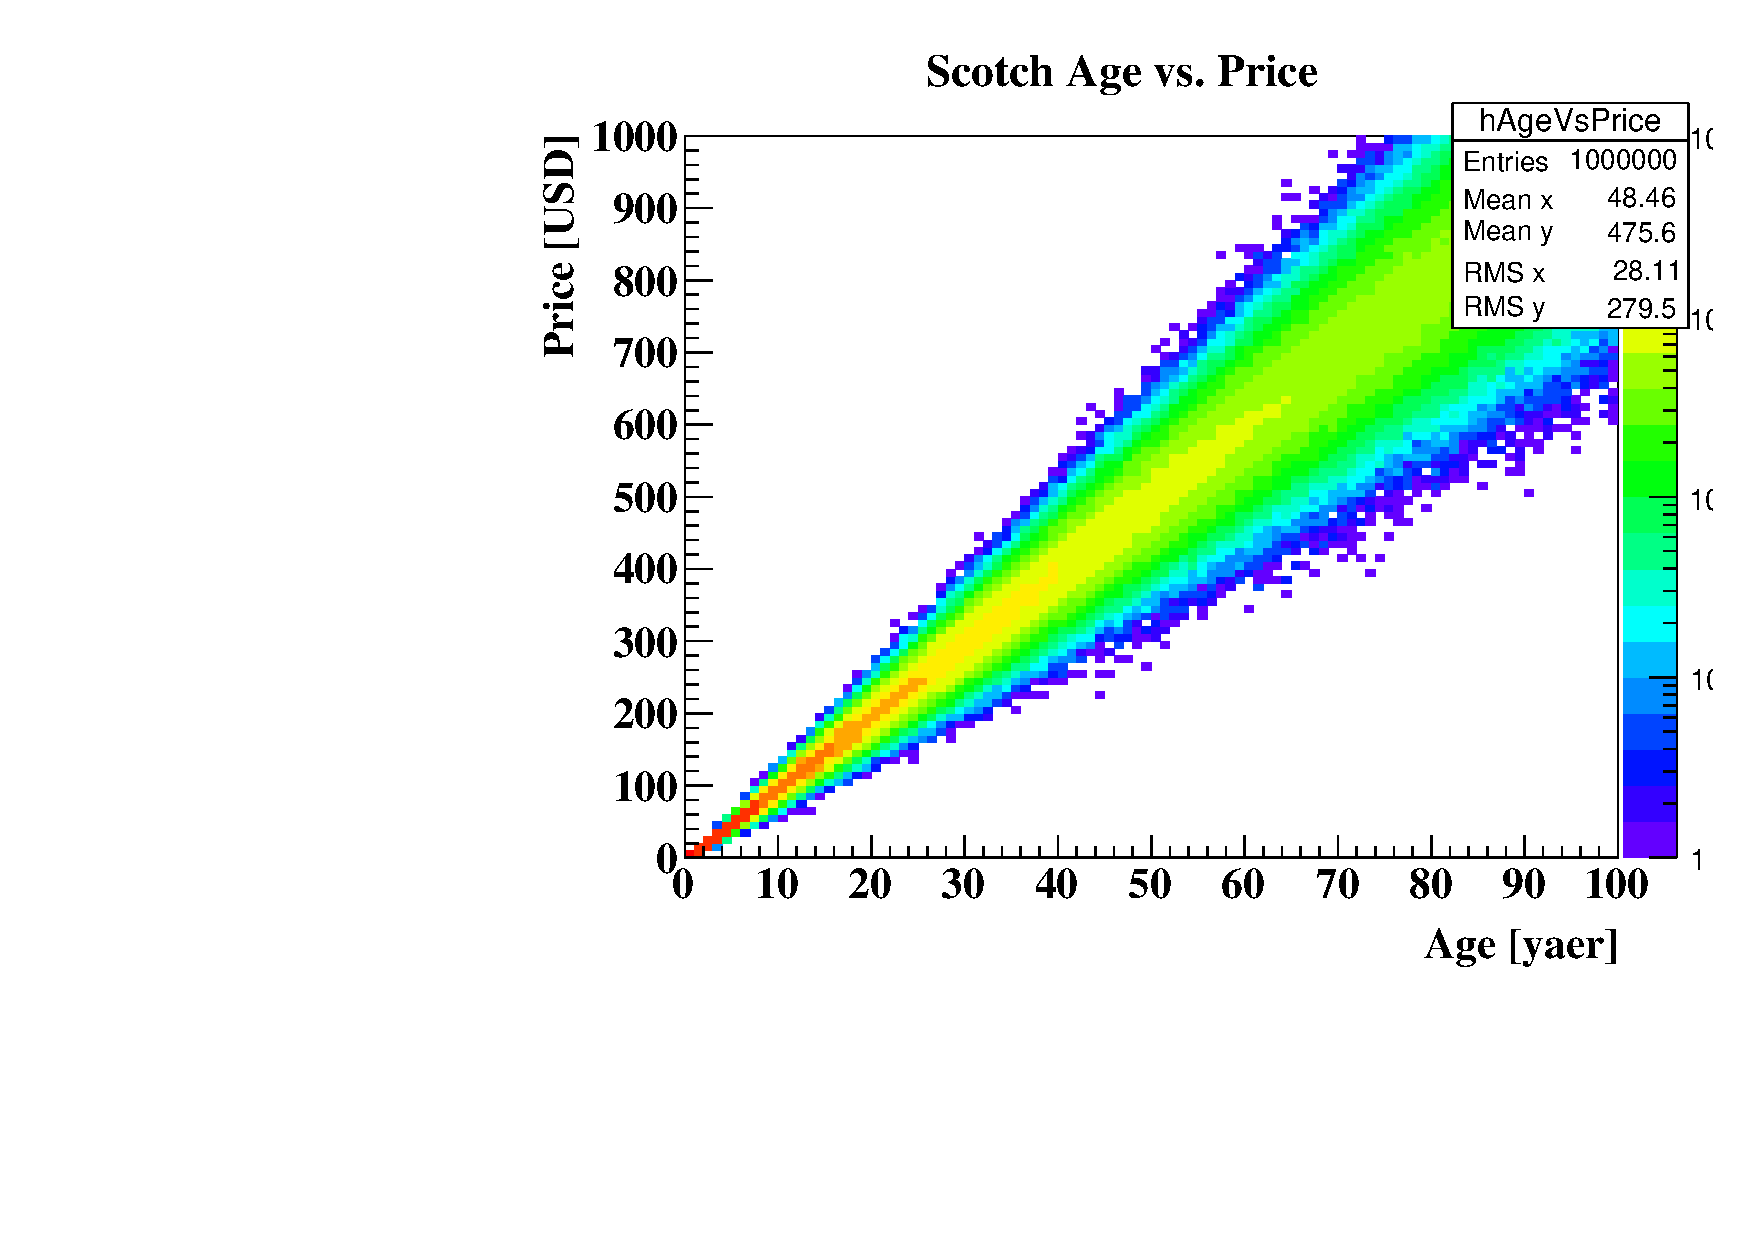
\includegraphics[width=12cm]{./img/ScotchAgeVsPrice.pdf}
\caption{ 
Drawing the age vs. price distribution of {\ttfamily example::Scotch} class from {\ttfamily TTree::Draw}.
}
\end{center}\end{figure}

An example script {\ttfamily mac/example.py} demonstrates how you can:
\begin{itemize}
\item Instantiate {\ttfamily example::Scotch} and save it in a \ROOT file
\item Create a {\ttfamily TTree} of {\ttfamily example::Scotch} for 1e6 entries and save
\item Read-in stored {\ttfamily TTree} and make a very simple access to the stored data product
\item Read-in stored {\ttfamily TTree} and call {\ttfamily TTree::Draw} on the stored data product
\end{itemize}

Note that storing multiple variables into a separate branch of {\ttfamily TTree} (i.e. Ntuple approach)
is much more tedious than storing a class instance as demonstrated in {\ttfamily Scotch::ShipScotch}
function. There, you can find a single line to create a {\ttfamily TTree} branch:
\begin{lstlisting}
tree.Branch("scotch",&data);
\end{lstlisting}
where ``data'' is a {\ttfamily example::Scotch} instance.
With this single line call, all variables in {\ttfamily example::Scotch} instance is stored
with a proper type, and will be readout correctly.

Another myth often people have is that it is very hard to access this object information from
{\ttfamily TTree}. As you can see in the {\ttfamily example.py}, this is completely irrelevant:
you can access the object directly via branch name. A single line in {\ttfamily Python} from
the script is shown below:
\begin{lstlisting}
ch.scotch.Speak()
\end{lstlisting}
which accesses the stored object and calling the class member function {\ttfamily example::Beer::Speak()}.

\subsection{Package Dependency}
The package {\ttfamily Example/Dependent} is prepared to demonstrate how one can make an inter-package 
dependency. In particular, this package depends on {\ttfamily Example/Function} package. Make sure
you have finished building {\ttfamily Example/Function} before building this package.

As you can see in {\ttfamily Stout.h}, the \CPP class {\ttfamily example::Stout} inherits from
{\ttfamily example::Beer}. In order to avoid re-compilation of {\ttfamily example::Beer} class,
we take a usual approach of just {\it linking} the libraries together. Take a look at 
{\ttfamily GNUmakefile}, in particular the following lines:
\begin{lstlisting}
...
INCFLAGS += -I$(LARLITE_USERDEVDIR)/Example
...
LDFLAGS += -L$(LARLITE_LIBDIR) -lExample_Function
\end{lstlisting}
As advertised in the previous section, you must include the path to find {\ttfamily Beer.h} (which
is called from {\ttfamily Stout.h} via {\ttfamily \#include ``Beer.h''}) in {\ttfamily INCFLAGS}, and
both a path and name of a library that contains {\ttfamily example::Beer} class definition in
{\ttfamily LDFLAGS}. 

An example script {\ttfamily mac/example.py} demonstrates an instantiation of {\ttfamily example::Stout}
class and also a call to its base class function {\ttfamily example::Beer::Speak()}.

\subsection{\python in \CPP}
Finally, some users are interested in developing \CPP code to directly operate on \python objects.
An example {\ttfamily Example/PyExample} is prepared to give a tip on how one can write a \CPP
API for \python. This is much better documented as a part of \python documentation:
\begin{center}
{\color{blue}\url{https://docs.python.org/2/c-api/}}
\end{center}

Using a native \python \CPP API is not very easy nor straight forward. Hence in this example,
again, we use \PyROOT binding that makes our life much easier. In short, a difference of two
methods is that you do not have to write your own binding, which is an extra code that has nothing
to do with your algorithm. Finally, that being said, there are other bindings available out there
such as {\ttfamily Cython} (... and \PyROOT uses one of them underneath anyways).

\subsubsection{External Dependnecy}
First of all, you will be using native \python classes, hence you will depend on \python.
Accordingly you have to modify {\ttfamily GNUmakefile}, in particular {\ttfamily INCFLAGS} and
{\ttfamily LDFLAGS}. Notice following 2 lines in {\ttfamily GNUmakefile}:
\begin{lstlisting}
...
INCFLAGS += $(shell python-config --includes)
...
LDFLAGS += $(shell python-config --ldflags)
\end{lstlisting}
each specifying an extra path to find a \python header file and libraries.

\subsubsection{Hiding \python Header From \CINT}
\python header file is called {\ttfamily Python.h}, and is not parse-able via \ROOT \CINT
compiler. So you have to hide it from \CINT dictionary generation step. This can be seen
in {\ttfamily PyExample.h} header file:
\begin{lstlisting}
...
#ifndef __CINT__
// You have to hide native Python header include from CINT                                                                                                                                                  
#include "Python.h"
#endif
...
\end{lstlisting}

You also need to provide two magic lines to forward declare types:
\begin{lstlisting}
...
struct _object;
typedef _object PyObject;
...
\end{lstlisting}
which is for \python generic object pointers to be used (this is a part of \python \CPP API).

\subsubsection{{\ttfamily example::PyExample::Convert}}
The example class {\ttfamily example::PyExample} has an example function to create a
\python list from a \CPP {\ttfamily std::vector<std::string>} object. You can look at the
source code as to how one can do this very simple operation, and take a look at \python
documentation for doing more elaborate operations.

Running {\ttfamily mac/example.py} should show you how this function works.
Obviously you may want to expand the code to work with more advanced \python objects
such as {\ttfamily numpy} array, {\ttfamily matplotlib} axis, and such. The author
does not have much experience to extend too far, but is happy to discuss if you need a help.

\subsection{Documenting Code Using {\ttfamily Doxygen}}
Though this is not everyone's favorite choice, {\ttfamily doxygen} is a popular method to
provide an in-line documentation in the source code. It works pretty nicely with \CPP, and
somewhat at acceptable level with \python. It is the recommended choice for LArSoft to provide
a minimal documentation.

LArLite repositories comes with a doxygen script. You can try generating a documentation
in {\ttfamily Example} directory by typing:
\begin{lstlisting}
  > make doxygen
\end{lstlisting}
({\bf you need doxygen installed in your system!}).

\begin{figure}[htb]\begin{center}
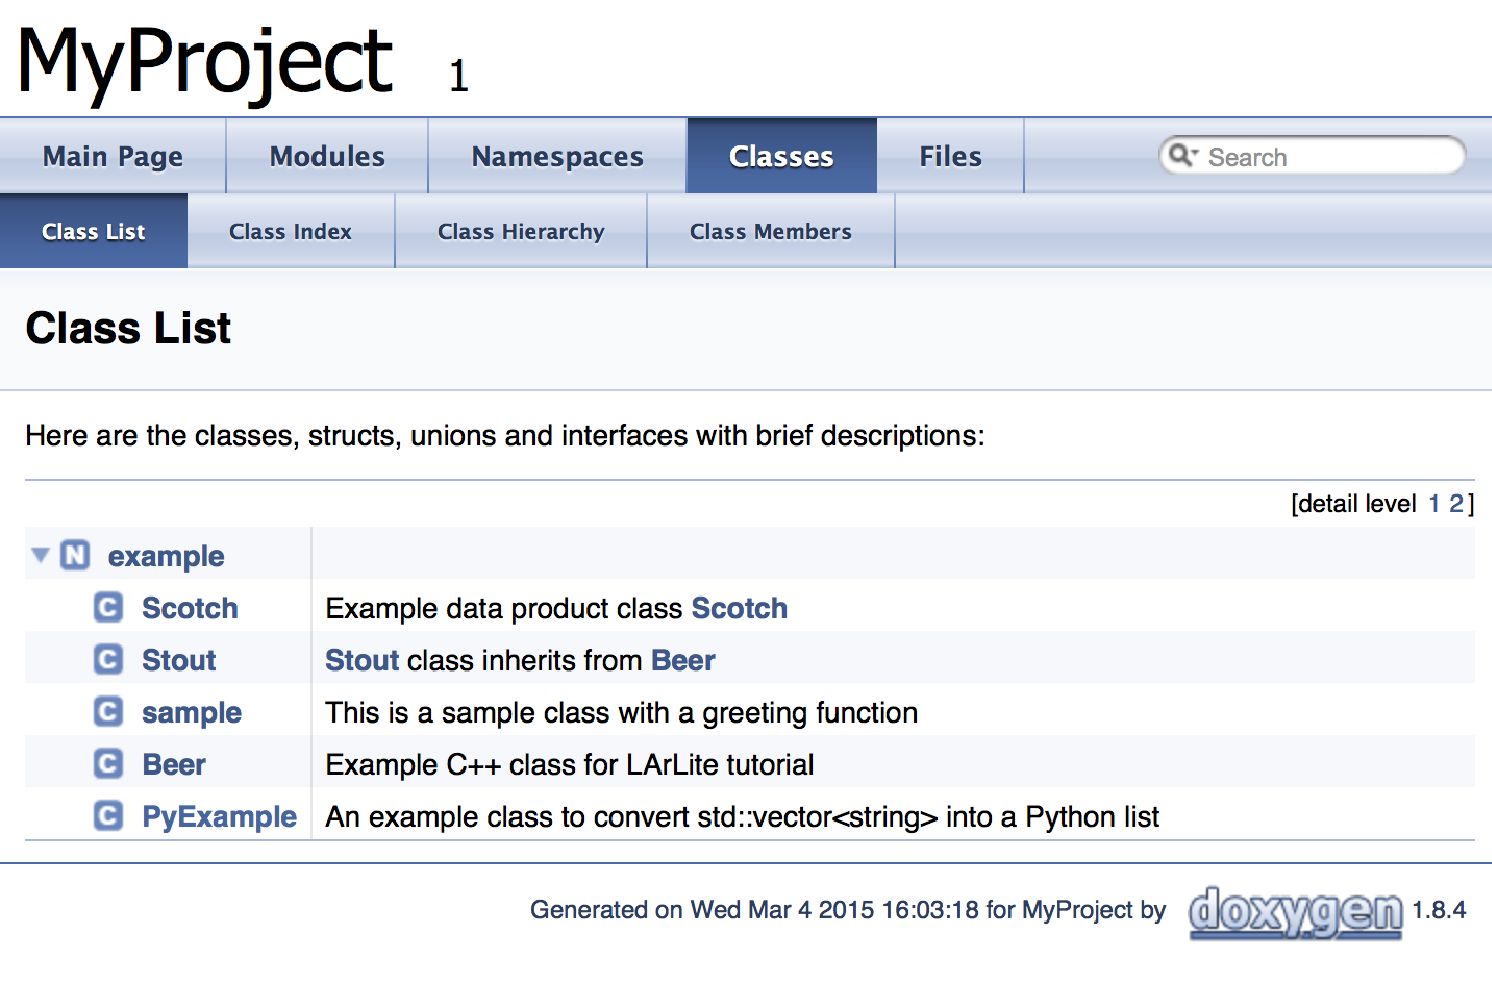
\includegraphics[width=12cm]{./img/doxygen.pdf}
\caption{ 
Doxygen web page generated by ``{\ttfamily make doxygen}'' command for {\ttfamily Example} repository.
}
\end{center}\end{figure}

After successfully running the above command, you should find a chain of HTML files 
to browse through (no internet needed). This way you can also check your doxygen comment
format (whether this is correct or not) before you commit the code. You can look at the
generated documentation using a command like below:
\begin{lstlisting}
  > firefox -a doc/dOxygenMyProject/html/index.html 
\end{lstlisting}
on {\ttfamily Linux} or
\begin{lstlisting}
  > open doc/dOxygenMyProject/html/index.html 
\end{lstlisting}
on {\ttfamily OSX}. The figure shows a generated documentation webpage on the author's laptop.

To understand {\ttfamily doxygen} comment style, refer to their web documentation:
\begin{center}
{\color{blue}\url{http://www.stack.nl/~dimitri/doxygen/manual/docblocks.html}}
\end{center}



% Overall introduction
\chapter{Introdcution}
\label{chap:introduction}

This chapter discuss about how to generating user's own code development space.
In particular following itmes are discussed in the respective order.
\begin{itemize}
\item Getting started: your own code repository
\item A simple \CPP project package 
\item Stuffing your package
\begin{itemize}
  \item Simple \CPP class
  \item \anaunit (see Ch.\ref{chap:analysis}).
  \item \ertool algorithm class (see \ertool documentation)
  \item \ertool filter class (see \ertool documentation)
  \item \ertool analysis class (see \ertool documentation)
  \item \CPP functions
\end{itemize}
\item Details: LArLite build basics
\item Advanced Code Development
\begin{itemize}
  \item \CPP functions outside classes
  \item Inter-package dependence
  \item Data product: storing \CPP class instance in \ROOT file
  \item \python in \CPP (i.e. opposite of \PyROOT)
\end{itemize}
\end{itemize}

\section{Creating Your Repository}
\label{sec:devrepo}

LArLite supports user code development under \UserDev.
More precisely, it is assumed to be under any path that is set to the value of shell environment variable {\ttfamily \$LARLITE\_USERDEVDIR}. 
For the sake of simplicity we stick with \UserDev in this section.

\subsection{Note About \UserDev}
Important note first:
\begin{itemize}
  \item {\ttfamily UserDev/GNUmakefile}, if it exists, is generated by setup.sh and it does not belong to LArLite repository (ignore it).
  \item Some sub-directories belong to LArLite (see below). Some of these depend on LArLite and some don't. It is useful to note them briefly here.
    \begin{itemize}
        \item {\ttfamily BasicTool} contains useful packages like {\ttfamily GeoAlgo} and has no dependency outside
        \item {\ttfamily SelectionTool} contains useful packages like {\ttfamily ERTool} and depends on {\ttfamily BasicTool}
        \item {\ttfamily RecoTool} contains shower reconstruction code and depends on {\ttfamily core}
        \item {\ttfamily LArLiteApp} contains LArLite application from {\ttfamily GeoAlgo} and {\ttfamily ERTool} 
    \end{itemize}
  \item You can create new directories under \UserDev and that won't bother other users. We'll do this below. 
  This is all done through {\ttfamily .gitignore} rule placed under the top directory. 
\end{itemize}

These features of \UserDev are there so that you feel more free to make a mess (sorry, I meant, to develop code) there!

\subsection{Creating Your Sub-Repository in \UserDev}
\label{sec:devrepo:makenew}
Obviously I cannot just say ``do whatever under \UserDev'' and leave: I would love to support a very easy way to develop code (or make a mess) under \UserDev. I will just show you how to do things here:
\begin{lstlisting}
     > llgen_repository MyRepo
\end{lstlisting}
where the execution command is an alias explained in Sec.\ref{sec:configure}.
This should create a new directory called {\ttfamily MyRepo} under \UserDev. 
That is your new repository. As said, this does not affect LArLite repository. 
If you don't want to keep {\ttfamily MyRepo}, simply ``{\ttfamily rm -r}'' it.

Another thing to note here: your repository will contain code and you will compile them, making a compiled shared object library. 
Your repository name will be used to name your library file (if you follow LArLite code generation scripts described in the followings). 
So pick a name that suits for your purpose. You do not want to pick a generic name that might coincide with some other libraries on your machine.

\subsection{What's in MyRepo?}

Your new repository comes with a GNUmakefile (which does nothing for now) and {\ttfamily doc} 
directory with a doxygen script but empty otherwise. Under this space, you can create your ``packages'' as a 
set of \CPP code to be compiled into a library. We will discuss about more later.

\subsection{Creating Your Sub-Repository in {\ttfamily github}}
In the previous section, we created a new repository {\ttfamily MyRepo} under \UserDev. But that's just a directory on your laptop, and you may want to keep it as your code repository using either {\ttfamily svn} or {\ttfamily github} (or anything else you would like to use). Here, I briefly mention how you can do this using {\ttfamily github} because it's very easy given that you already have a {\ttfamily github} account.

First of all, go to {\ttfamily github.com} and create your own repository: go to your {\ttfamily github} account web page, and click on ``+'' symbol that is toward right-top of the web page. Choose ``New repository''. Then enter the repository name you are about to create. Ideally you may want to choose a somewhat unique name as described in Sec.\ref{sec:devrepo:makenew}. You can always remove your repository if you don't like it.

Then checkout your empty repository. As an example, I use my empty repo called {\ttfamily EmptyRepo}.
\begin{lstlisting}
    > cd $LARLITE_USERDEVDIR
    > git clone git@github.com:drinkingkazu/EmptyRepo EmptyRepo
\end{lstlisting}
Now simply run:
\begin{lstlisting}
    > python bin/gen_new_repository EmptyRepo
    > cd EmptyRepo
    > git add .
    > git commit -m ``new repository''
    > gitpush -u origin master
\end{lstlisting}
and you are done!
From the next time, if you want to install LArLite from scratch, simply checkout your repository under UserDev with the same name.

As said many times, of course, your repository is independent of LArLite repository.





\section{Creating a Package}
\label{sec:package}
Here, I assume we are working under {\ttfamily UserDev/MyRepo}. 
In fact, since it's tedious, I will just refer to {\ttfamily MyRepo}.

\subsection{What is a ``Package''?}
``Package'' is a directory under a repository that is compiled and generates one {\bf shred object library}
(i.e. a file with {\ttfamily .so} extension). This library is loaded at a run-time or linked via compiler as one byte code file.
This gives you a sense of what to include in one package: having too many classes (and especially unrelated classes) in one package
means an extra overhead cost for a run-time loading or linking at compilation. In other words, you probably do not want make one 
library per class, but also not one library for all classes. A package should contain a group of \CPP classes/functions which you
think it makes sense to put together.

\subsection{Making a Simple \CPP Package}

Like advertised many times, LArLite was originally a \CPP project play ground for summer students. 
The author thinks it's very important to have an empty \CPP package generator that comes with build system, 
so that a user can focus on writing the algorithm instead of figuring out how to compile and such.

So here it is: there is a \python script to generate an empty \CPP package:
\begin{lstlisting}
    $LARLITE_BASEDIR/bin/gen_package
\end{lstlisting}
This script takes one input argument which is used to name a ``package'', a directory to be created under {\ttfamily MyRepo}.
This script {\bf needs to be executed somewhere under {\ttfamily MyRepo}} (otherwise you'll see an error message).
One can run this script via alias:
\begin{lstlisting}
    > llgen_package MyProject
\end{lstlisting}
which will create a directory {\ttfamily MyRepo/MyProject} that include minimal set of source codes to compile an empty \CPP class. 
You can have your name choice in place of ``MyProject''. After running the command, try:
\begin{lstlisting}
    > cd MyProject
    > make -j4
\end{lstlisting}
This compiles your code and makes {\ttfamily libMyRepo\_MyProject.so} under {\ttfamily lib} directory.
What you compiled is a \CPP class called ``sample'' defined in {\ttfamily sample.h}. 


\subsection{Using in Interpreter}

So how can you ``use'' this \CPP class? You can write a binary executable code, or try out in \CINT or \PyROOT. Here is an example:
\begin{lstlisting}
    > root
    root[0] sample k;
\end{lstlisting}
Above lines work (i.e. your class instance is created) because \CINT is informed about your class. 

\subsection{``Hello World'' Development}
\label{sec:helloworld}
Let's try a simple modification to your class. Here's an example ``hello world'' program using \CPP class. Open {\ttfamily sample.h} and add a {\ttfamily void} function as shown below:
\begin{lstlisting}
class sample{
public:
  /// Default constructor
  sample(){};
  /// Default destructor
  virtual ~sample(){};
  /// Hello world!
  void HelloWorld() { std::cout << ``Hello World!'' << std::endl; }
};
\end{lstlisting}
Save, close and compile (i.e. type ``make''). Now, try the following in \CINT or \PyROOT:
\begin{lstlisting}
    > root
    root[0] sample k;
    root[1] k.HelloWorld();
    Hello World!
    root[2]
\end{lstlisting}

Whenever you want to start a new project with an empty class, you can come back to this example and create your new \CPP project!





\section{Adding Basic \CPP Classes}
\label{sec:expand_package}

As discussed in the previous section, one should populate a package with a group of \CPP classes.
This section describes how to add various types of \CPP classes to your package.

\subsection{Simple \CPP Class}
Sometimes (rather often) you want to generate a completely generic \CPP class for very good reasons: to develop 
some algorithm that is independent of the framework (= easy portability to outside LArLite).

Here is a script for you:
\begin{lstlisting}
    > cd $LARLITE_USERDEVDIR/MyRepo/MyProject
    > llgen_class_empty MyEmptyClass
\end{lstlisting}
Now you should see {\ttfamily MyEmptyClass.h} and {\ttfamily MyEmptyClass.cxx} created under {\ttfamily MyAna}
package. There also made appropriate modification to {\ttfamily LinkDef.h} so that you can just type:
\begin{lstlisting}
    > make -j2
\end{lstlisting}
to compile your new class. Now develop your awesome algorithm and make it a non-empty class ;)

\subsection{\anaunit Class}
If you wish to generate an empty \anaunit class code (to be implemented by you), simply try:
\begin{lstlisting}
    > cd $LARLITE_USERDEVDIR/MyRepo/MyProject
    > llgen_class_anaunit MyAna
\end{lstlisting}

Executing above commands create {\ttfamily MyAna.cxx} and {\ttfamily MyAna.h} (and an appropriate modification to {\ttfamily LinkDef.h}).
Try:
\begin{lstlisting}
    > make -j4
\end{lstlisting}
You just made your new \anaunit class, {\ttfamily MyAna}, whieh inherits from {\ttfamily ana\_base}! 
Your new \anaunit is accessible from \CINT or \PyROOT like any other classes in LArLite:
\begin{lstlisting}
    > root
    root[0] larlite::MyAna my_ana_instance
\end{lstlisting}
Now go ahead and code up this analysis unit, and run with {\ttfamily ana\_processor}! 

\subsubsection{Run Your Analysis Unit: \PyROOT}
\label{sec:yourrunscript}
There is an example \python run script for \anaunit under {\ttfamily mac} directory, called 
{\ttfamily example\_anaunit.py}. You need a LArLite sample \ROOT file to run this program. 
If you have a sample file, say {\ttfamily trial.root}, you can run the program as follows.
\begin{lstlisting}
    > python mac/example_anaunit.py trial.root
\end{lstlisting}

\subsection{\ertool Classes}
Just as we exercised how to add a new \CPP class to a package, there's analogous python scripts to
generate \ertool reconstruction algorithm, filter, and analysis class:
\begin{lstlisting}
    > cd $LARLITE_USERDEVDIR/MyRepo/MyProject
    > llgen_class_erfilter Trial
    > llgen_class_eralgo Trial
    > llgen_class_erana Trial
\end{lstlisting}
Above three commands generate three \CPP classes: {\ttfamily ERFilterTrial}, {\ttfamily ERAlgoTrial}, and {\ttfamily ERAnaTrial}.
These are implementation of base classes defined in \ertool, hence must be used with {\ttfamily ertool::Manager}.
For details, see \ertool documentation (which is to come...)






\section{Understanding the Build}
\label{sec:build_package}
This section covers the basics of how the LArLite build works, aiming to reduce a black-box content for users and developers.
The following topics are ordered such that a topic of interest to more people gets covered first.

\subsection{{\ttfamily Compiler} and {\ttfamily Linker} for Dummies}
Skip if you already know about them, obviously.

Our \CPP source codes are merely descriptions of what we want our computer to do in human-friendly language 
(disagree on ``human-fiendly''? Welcome to the club).
A {\ttfamily compiler} takes in our source code and generate a machine-friendly description, often called as an {\it object file} or {\it byte code}.
When you compile your package in LArLite, you find files with {\ttfamily .o} extension: these are the object files.

Now having many granular object files is not very helpful.
A {\ttfamily linker} allows us to combine multiple object files and create a {\it shared object library} file.
You find such files with {\ttfamily .so} extension under {\ttfamily \$LARLITE\_LIBDIR} if you compiled any package.
The scope of what objects should be put together is really a developer's choice.
In LArLite, this is done per package.
Another (and more important) advantage of shared object libraries kicks in when you compile another code that depends on it.
Say you have a \CPP class {\ttfamily A} and {\ttfamily B} where {\ttfamily B} depends on {\ttfamily A}. 
Once you have {\ttfamily A} compiled with {\ttfamily .so} file, a separate compilation of {\ttfamily B} does not require
a re-compilation of {\ttfamily A}'s source code. Instead, you can {\it link} the {\ttfamily A}'s library upon compilation
of {\ttfamily B}'s library.

In LArLite, we compile files with {\ttfamily .cxx} extensions with a compiler, and create a shared object library using a linker, which
is nothing special compared to any other softwares' build system.

\subsection{{\ttfamily INCFLAGS} and {\ttfamily LDFLAGS}: LArLite Compiler Flags}
In LArLite package's {\ttfamily GNUmakefile}, you may see variables named as {\ttfamily INCFLAGS} and {\ttfamily LDFLAGS} where
the latter may not appear in some simple code packages (i.e. don't worry about not seeing {\ttfamily LDFLAGS} in your {\ttfamily GNUmakefile}).
These are called {\it compiler flags} and passed onto a compiler and linker respectively.

\subsubsection{INCFLAGS}
{\ttfamily INCFLAGS} is used by a compiler to search for files you specify with {\ttfamily \#include} preprocessor command in your source code.
In other words, if your source code calls {\ttfamily \#include <TH1D.h>}, then the directory path which contains {\ttfamily TH1D.h} has to be
added to {\ttfamily INCFLAGS}. The format of {\ttfamily INCFLAGS} is ``-I\$PATH'' where you should replace ``\$PATH'' with the relevant
directory path.

That being said, by default, LArLite includes a \ROOT's include flags.
\ROOT follows a standard method to provide such flags, and you can try this in your installation as well:
\begin{lstlisting}
  > root-config --cflags
\end{lstlisting}
The output of above command is a part of LArLite's default {\ttfamily INCFLAGS}.

\subsubsection{LDFLAGS}
{\ttfamily LDFLAGS} is used by a linker to find libraries to be linked into your package. If your package depends on any externaly compiled
code, for instance a \ROOT class {\ttfamily TH1D}, you have to specify the library to be linked here. The format is 
{\ttfamily -L\$PATH -l\$LIBNAME} where ``\$PATH'' is the directory path that contains a library named ``lib\$LIBNAME.so''. Note that
you should exclude the prefix ``lib'' when you specify it in {\ttfamily LDFLAGS} as that is the standard of how a linker takes in library names.

The default flags in LArLite includes a \ROOT's library flags.
Again, as it was the case for {\ttfamily INCFLAGS}, you can try:
\begin{lstlisting}
  > root-config --libs
\end{lstlisting}
which include most of standard \ROOT libraries such as IO, histogram, TTree, TMatrix, TVector3, etc.

\subsubsection{Flags for LArLite Packages}
You may write a package that depends on existing LArLite code.
One example is an analysis code that inherits from {\ttfamily lalrite::ana\_base}. 
Then you will have to specify {\ttfamily INCFLAGS} and {\ttfamily LDFLAGS}.

Specifying every single {\ttfamily INCFLAGS} and {\ttfamily LDFLAGS} for LArLite code is definitely annoying.
So we follow the popular standard and the following scripts are prepared:
\begin{itemize}
\item {\ttfamily larlite-config} for LArLite's analysis framework
\item {\ttfamily basictool-config} for code under \UserDev/BasicTool 
\item {\ttfamily seltool-config} for code under \UserDev/SelectionTool
\item {\ttfamily recotool-config} for code under \UserDev/RecoTool
\end{itemize}
These scripts can be run with either {\ttfamily --includes} or {\ttfamily --libs} option, and they
simply prints out relevant string to be added to {\ttfamily INCFLAGS} and {\ttfamily LDFLAGS} respectively.
For instance, you may try:
\begin{lstlisting}
  INCFLAGS += $(shell larlite-config --includes)
\end{lstlisting}
and/or
\begin{lstlisting}
  LDFLAGS += $(shell larlite-config --libs)
\end{lstlisting}
in your {\ttfamily GNUmakefile}.

If you use {\ttfamily gen\_class\_anaunit} or similar script, actually, this modification to a {\ttfamily GNUmakefile} is done
by the same script. Hence you do not need to worry about it.

\subsection{Compiler \& Linker Used by LArLite}
Let me make a brief note on how compiler/linker is picked and what default compiler/linker flags are set for LArLite build.

When possible LArLite attempts to use \clang++. In particular this is searched and set when one runs {\ttfamily setup.sh} script.
The configured compiler name is set to a shell environment variable {\ttfamily \$LARLITE\_CXX}.
Further, compiler/linker specific flags are defined in:
\begin{lstlisting}
  > $LARLITE_BASEDIR/Makefile/Makefile.X
\end{lstlisting}
where {\ttfamily X} may be either ``Darwin'' or ``Linux''. 


\section{Advanced Development}
\label{sec:advanced_package}

In this section we follow a prepared example that can be found in:
\begin{center}
{\color{blue}\url{https://github.com/drinkingkazu/Example}}
\end{center}
You might have already checked out this repository as this was mentioned briefly
in the introductory section (see Sec.\ref{sec:build}). 
If not, can certainly checkout under \UserDev:
\begin{lstlisting}
  > cd $LARLITE_USERDEVDIR
  > git clone https://github.com/drinkingkazu/Example
\end{lstlisting}

This repository contains following packages:
\begin{itemize}
\item {\ttfamily Empty} for the simplest example to introduce a simple \CPP class
\item {\ttfamily Function} for demonstrating a \CPP function to be exported into a dictionary
\item {\ttfamily Dependent} for showing how to make inter-package dependencies
\item {\ttfamily DataProduct} as an example of how to store a class instance into a file
\end{itemize}
where we skip the first item, {\ttfamily Empty}, as that has been covered in the previous section.

\subsection{\CPP Functions}
I would like to avoid a confusion: \CPP class is an extension of data structure. In particular,
you do not have to make \CPP class for inventing one or a few functions. Just like we have done
some practice with \CPP class, it would be useful to have \CPP functions in a dictionary.
The point of this package is to show how one can do this.

Take a look at {\ttfamily MyFunctions.h} and {\ttfamily MyFunctions.cxx} source code: there, I defined
functions:
\begin{lstlisting}
  void hello_world();
  Beer Brew(const int age);
\end{lstlisting}
where {\ttfamily example::Beer} is a \CPP class defined in {\ttfamily Beer.h}: it's very very simple class for
playing around unlike the sophisticated name.

Now a compilation works just as expected, and there is nothing special about these functions.
What you may find useful is a format to declare above functions in {\ttfamily LinkDef.h}:
\begin{lstlisting}
#pragma link C++ function  example::hello_world()+;
#pragma link C++ function  example::Brew(const int)+;
\end{lstlisting}
As you can see, a) you do not specify the return type of the function, and b) you only need to specify
the argument types. 

You can try executing an example script {\ttfamily mac/example.py} which calls those functions. 
Take a look at the script's contents and see if that makes sense (... and ask a question if you have any!).
{\color{red}\bf There is one caveat}, however: currently \ROOT seems to require \CPP class compiled
in the same library to be instantiated {\bf before} \CPP functions to be called. The author will
open a ticket for this to be fixed.

\subsection{\ROOT Data Product Class}
Once you get familiar with all LArLite features, you might want to store \CPP object in a file
as a {\ttfamily data product}. The easiest (and recommended) method is to use a \ROOT file.
A rule of the thumb is that any \CPP class that is generated with a \ROOT {\it dictionary} can
be stored in a \ROOT file. You can find details in the \ROOT manual.

If you use LArLite as your code development environment, \ROOT dictionary file is always
generated and built at compilation stage of your package. 

An example can be found in the package {\ttfamily DataProduct}.
There, a data product class called {\ttfamily example::Scotch} is defined. 

\begin{figure}[htb]\begin{center}
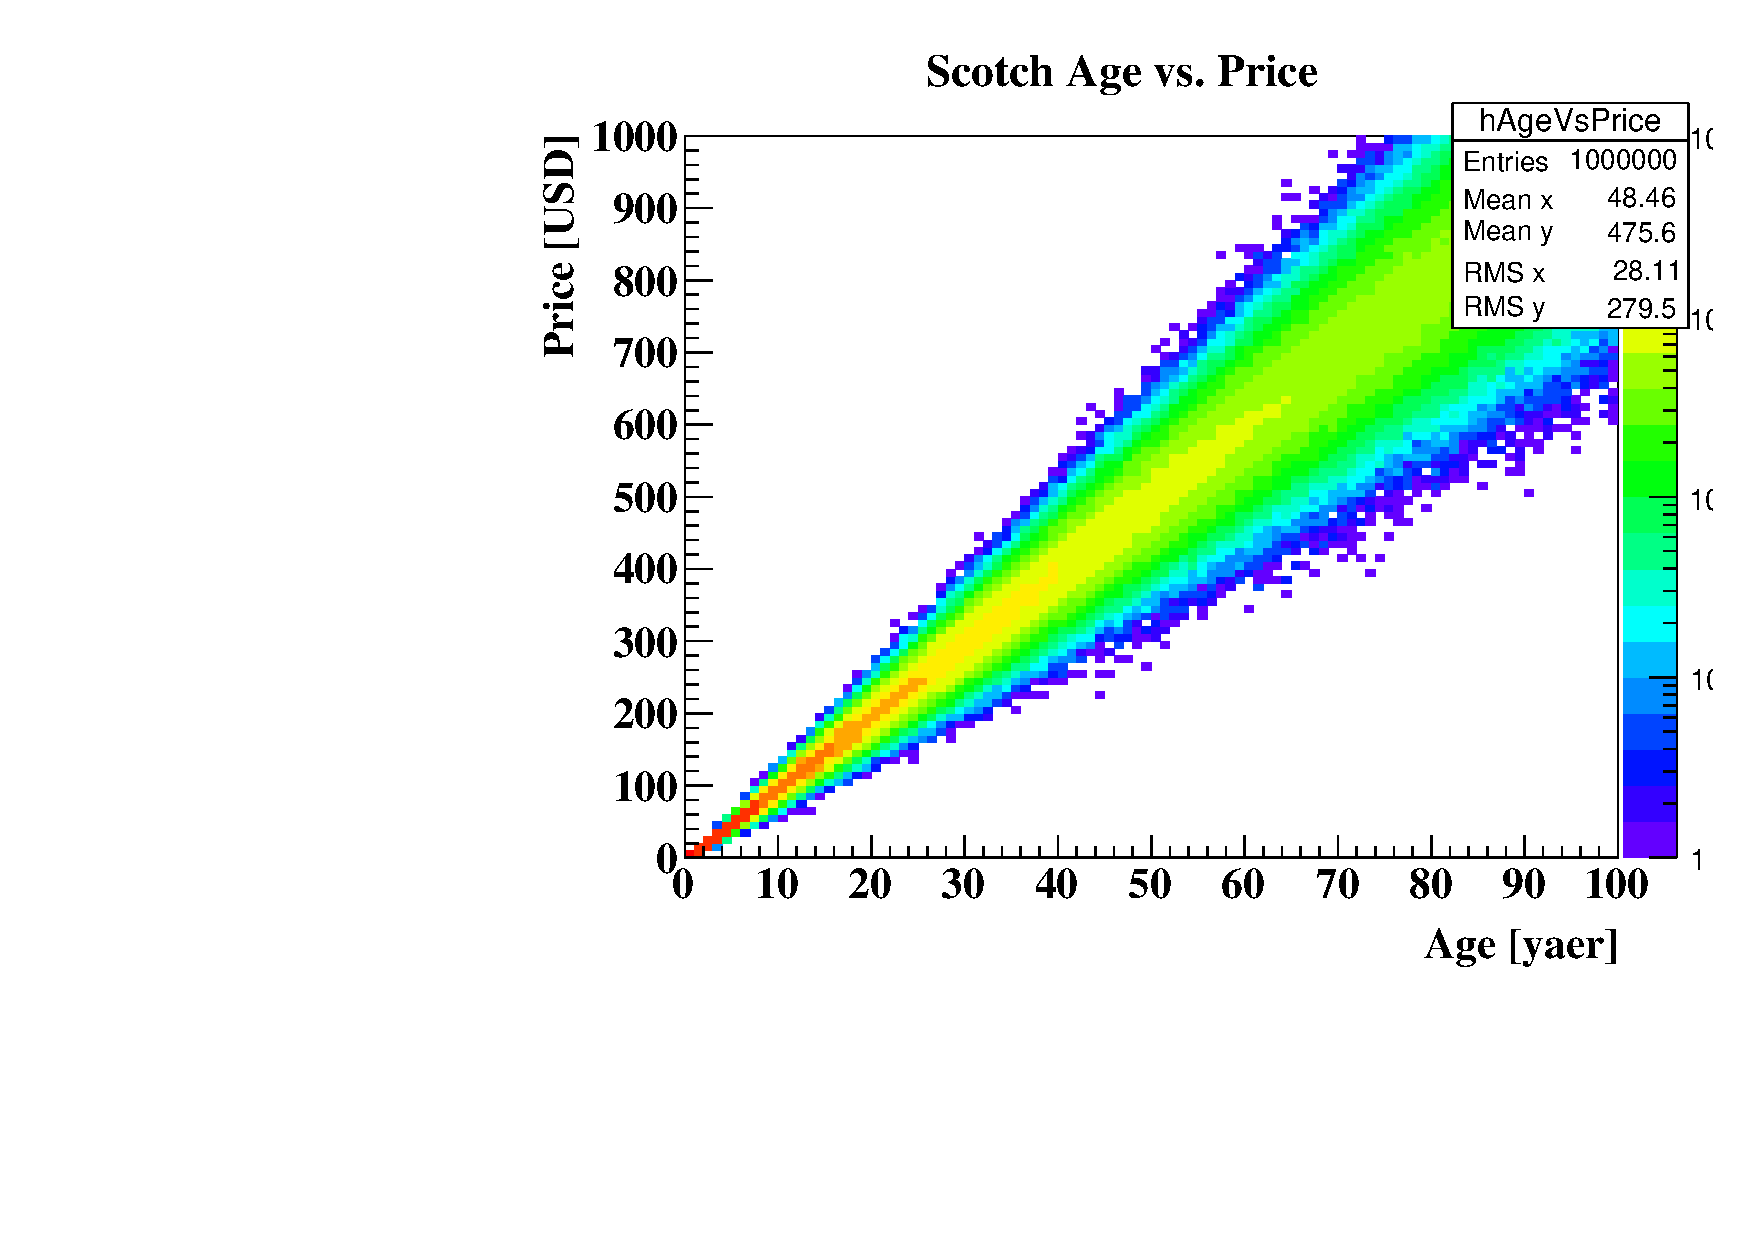
\includegraphics[width=12cm]{./img/ScotchAgeVsPrice.pdf}
\caption{ 
Drawing the age vs. price distribution of {\ttfamily example::Scotch} class from {\ttfamily TTree::Draw}.
}
\end{center}\end{figure}

An example script {\ttfamily mac/example.py} demonstrates how you can:
\begin{itemize}
\item Instantiate {\ttfamily example::Scotch} and save it in a \ROOT file
\item Create a {\ttfamily TTree} of {\ttfamily example::Scotch} for 1e6 entries and save
\item Read-in stored {\ttfamily TTree} and make a very simple access to the stored data product
\item Read-in stored {\ttfamily TTree} and call {\ttfamily TTree::Draw} on the stored data product
\end{itemize}

Note that storing multiple variables into a separate branch of {\ttfamily TTree} (i.e. Ntuple approach)
is much more tedious than storing a class instance as demonstrated in {\ttfamily Scotch::ShipScotch}
function. There, you can find a single line to create a {\ttfamily TTree} branch:
\begin{lstlisting}
tree.Branch("scotch",&data);
\end{lstlisting}
where ``data'' is a {\ttfamily example::Scotch} instance.
With this single line call, all variables in {\ttfamily example::Scotch} instance is stored
with a proper type, and will be readout correctly.

Another myth often people have is that it is very hard to access this object information from
{\ttfamily TTree}. As you can see in the {\ttfamily example.py}, this is completely irrelevant:
you can access the object directly via branch name. A single line in {\ttfamily Python} from
the script is shown below:
\begin{lstlisting}
ch.scotch.Speak()
\end{lstlisting}
which accesses the stored object and calling the class member function {\ttfamily example::Beer::Speak()}.

\subsection{Package Dependency}
The package {\ttfamily Example/Dependent} is prepared to demonstrate how one can make an inter-package 
dependency. In particular, this package depends on {\ttfamily Example/Function} package. Make sure
you have finished building {\ttfamily Example/Function} before building this package.

As you can see in {\ttfamily Stout.h}, the \CPP class {\ttfamily example::Stout} inherits from
{\ttfamily example::Beer}. In order to avoid re-compilation of {\ttfamily example::Beer} class,
we take a usual approach of just {\it linking} the libraries together. Take a look at 
{\ttfamily GNUmakefile}, in particular the following lines:
\begin{lstlisting}
...
INCFLAGS += -I$(LARLITE_USERDEVDIR)/Example
...
LDFLAGS += -L$(LARLITE_LIBDIR) -lExample_Function
\end{lstlisting}
As advertised in the previous section, you must include the path to find {\ttfamily Beer.h} (which
is called from {\ttfamily Stout.h} via {\ttfamily \#include ``Beer.h''}) in {\ttfamily INCFLAGS}, and
both a path and name of a library that contains {\ttfamily example::Beer} class definition in
{\ttfamily LDFLAGS}. 

An example script {\ttfamily mac/example.py} demonstrates an instantiation of {\ttfamily example::Stout}
class and also a call to its base class function {\ttfamily example::Beer::Speak()}.

\subsection{\python in \CPP}
Finally, some users are interested in developing \CPP code to directly operate on \python objects.
An example {\ttfamily Example/PyExample} is prepared to give a tip on how one can write a \CPP
API for \python. This is much better documented as a part of \python documentation:
\begin{center}
{\color{blue}\url{https://docs.python.org/2/c-api/}}
\end{center}

Using a native \python \CPP API is not very easy nor straight forward. Hence in this example,
again, we use \PyROOT binding that makes our life much easier. In short, a difference of two
methods is that you do not have to write your own binding, which is an extra code that has nothing
to do with your algorithm. Finally, that being said, there are other bindings available out there
such as {\ttfamily Cython} (... and \PyROOT uses one of them underneath anyways).

\subsubsection{External Dependnecy}
First of all, you will be using native \python classes, hence you will depend on \python.
Accordingly you have to modify {\ttfamily GNUmakefile}, in particular {\ttfamily INCFLAGS} and
{\ttfamily LDFLAGS}. Notice following 2 lines in {\ttfamily GNUmakefile}:
\begin{lstlisting}
...
INCFLAGS += $(shell python-config --includes)
...
LDFLAGS += $(shell python-config --ldflags)
\end{lstlisting}
each specifying an extra path to find a \python header file and libraries.

\subsubsection{Hiding \python Header From \CINT}
\python header file is called {\ttfamily Python.h}, and is not parse-able via \ROOT \CINT
compiler. So you have to hide it from \CINT dictionary generation step. This can be seen
in {\ttfamily PyExample.h} header file:
\begin{lstlisting}
...
#ifndef __CINT__
// You have to hide native Python header include from CINT                                                                                                                                                  
#include "Python.h"
#endif
...
\end{lstlisting}

You also need to provide two magic lines to forward declare types:
\begin{lstlisting}
...
struct _object;
typedef _object PyObject;
...
\end{lstlisting}
which is for \python generic object pointers to be used (this is a part of \python \CPP API).

\subsubsection{{\ttfamily example::PyExample::Convert}}
The example class {\ttfamily example::PyExample} has an example function to create a
\python list from a \CPP {\ttfamily std::vector<std::string>} object. You can look at the
source code as to how one can do this very simple operation, and take a look at \python
documentation for doing more elaborate operations.

Running {\ttfamily mac/example.py} should show you how this function works.
Obviously you may want to expand the code to work with more advanced \python objects
such as {\ttfamily numpy} array, {\ttfamily matplotlib} axis, and such. The author
does not have much experience to extend too far, but is happy to discuss if you need a help.

\subsection{Documenting Code Using {\ttfamily Doxygen}}
Though this is not everyone's favorite choice, {\ttfamily doxygen} is a popular method to
provide an in-line documentation in the source code. It works pretty nicely with \CPP, and
somewhat at acceptable level with \python. It is the recommended choice for LArSoft to provide
a minimal documentation.

LArLite repositories comes with a doxygen script. You can try generating a documentation
in {\ttfamily Example} directory by typing:
\begin{lstlisting}
  > make doxygen
\end{lstlisting}
({\bf you need doxygen installed in your system!}).

\begin{figure}[htb]\begin{center}
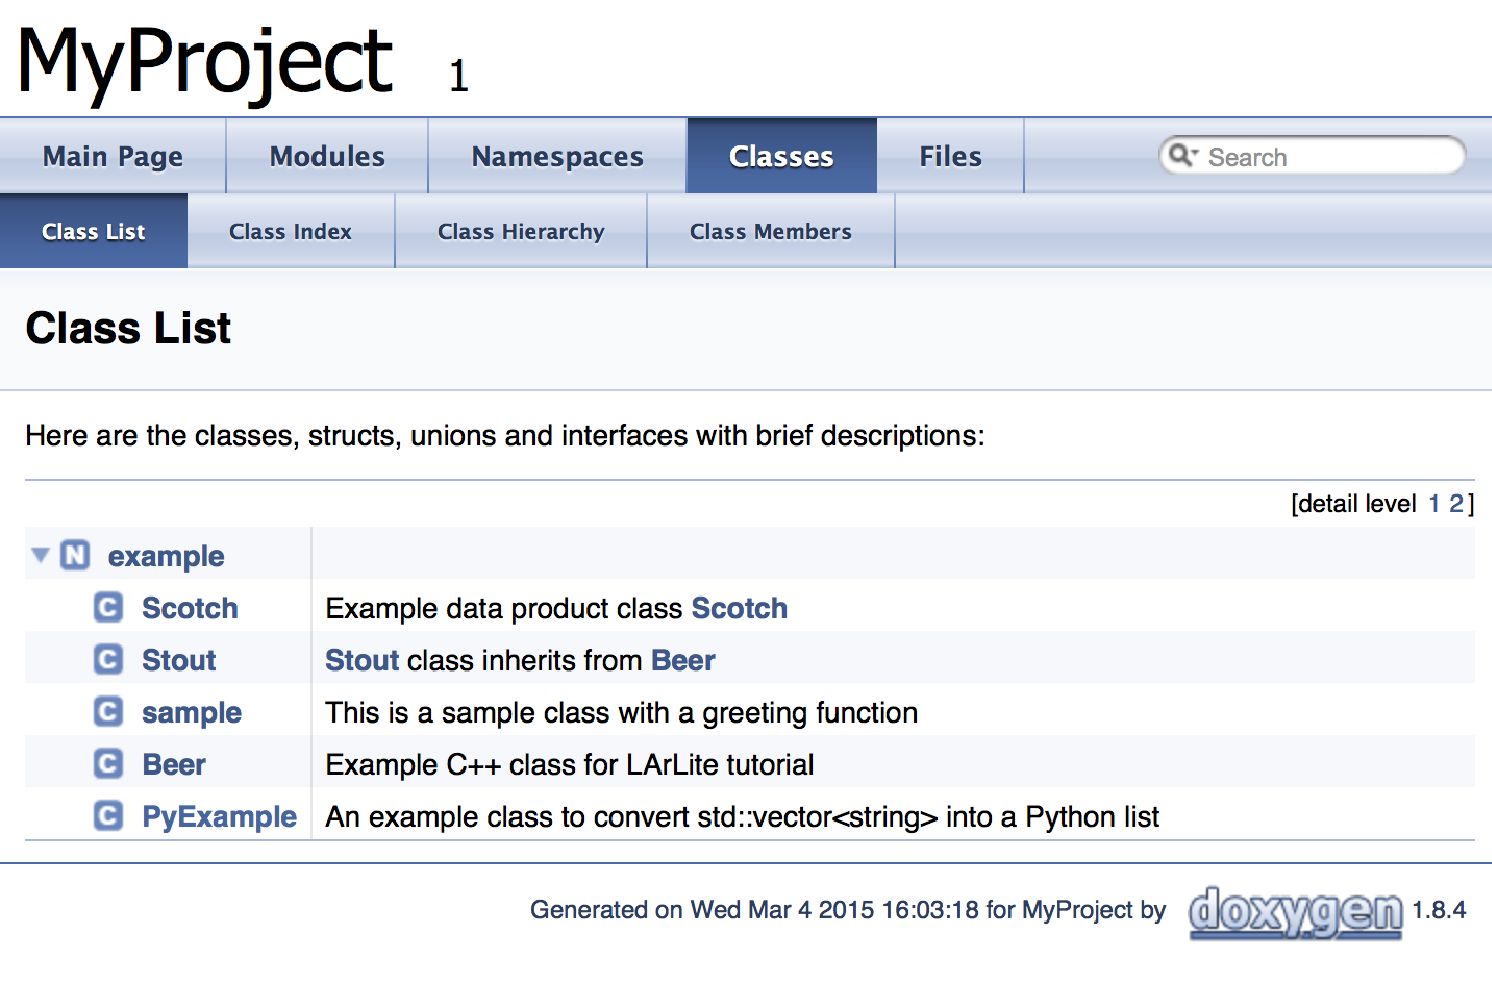
\includegraphics[width=12cm]{./img/doxygen.pdf}
\caption{ 
Doxygen web page generated by ``{\ttfamily make doxygen}'' command for {\ttfamily Example} repository.
}
\end{center}\end{figure}

After successfully running the above command, you should find a chain of HTML files 
to browse through (no internet needed). This way you can also check your doxygen comment
format (whether this is correct or not) before you commit the code. You can look at the
generated documentation using a command like below:
\begin{lstlisting}
  > firefox -a doc/dOxygenMyProject/html/index.html 
\end{lstlisting}
on {\ttfamily Linux} or
\begin{lstlisting}
  > open doc/dOxygenMyProject/html/index.html 
\end{lstlisting}
on {\ttfamily OSX}. The figure shows a generated documentation webpage on the author's laptop.

To understand {\ttfamily doxygen} comment style, refer to their web documentation:
\begin{center}
{\color{blue}\url{http://www.stack.nl/~dimitri/doxygen/manual/docblocks.html}}
\end{center}


 
% Base package description
\chapter{Core Package: Base}
\label{chap:base}

This chapter discuss about how to generating user's own code development space.
In particular following itmes are discussed in the respective order.
\begin{itemize}
\item Getting started: your own code repository
\item A simple \CPP project package 
\item Stuffing your package
\begin{itemize}
  \item Simple \CPP class
  \item \anaunit (see Ch.\ref{chap:analysis}).
  \item \ertool algorithm class (see \ertool documentation)
  \item \ertool filter class (see \ertool documentation)
  \item \ertool analysis class (see \ertool documentation)
  \item \CPP functions
\end{itemize}
\item Details: LArLite build basics
\item Advanced Code Development
\begin{itemize}
  \item \CPP functions outside classes
  \item Inter-package dependence
  \item Data product: storing \CPP class instance in \ROOT file
  \item \python in \CPP (i.e. opposite of \PyROOT)
\end{itemize}
\end{itemize}

\section{Creating Your Repository}
\label{sec:devrepo}

LArLite supports user code development under \UserDev.
More precisely, it is assumed to be under any path that is set to the value of shell environment variable {\ttfamily \$LARLITE\_USERDEVDIR}. 
For the sake of simplicity we stick with \UserDev in this section.

\subsection{Note About \UserDev}
Important note first:
\begin{itemize}
  \item {\ttfamily UserDev/GNUmakefile}, if it exists, is generated by setup.sh and it does not belong to LArLite repository (ignore it).
  \item Some sub-directories belong to LArLite (see below). Some of these depend on LArLite and some don't. It is useful to note them briefly here.
    \begin{itemize}
        \item {\ttfamily BasicTool} contains useful packages like {\ttfamily GeoAlgo} and has no dependency outside
        \item {\ttfamily SelectionTool} contains useful packages like {\ttfamily ERTool} and depends on {\ttfamily BasicTool}
        \item {\ttfamily RecoTool} contains shower reconstruction code and depends on {\ttfamily core}
        \item {\ttfamily LArLiteApp} contains LArLite application from {\ttfamily GeoAlgo} and {\ttfamily ERTool} 
    \end{itemize}
  \item You can create new directories under \UserDev and that won't bother other users. We'll do this below. 
  This is all done through {\ttfamily .gitignore} rule placed under the top directory. 
\end{itemize}

These features of \UserDev are there so that you feel more free to make a mess (sorry, I meant, to develop code) there!

\subsection{Creating Your Sub-Repository in \UserDev}
\label{sec:devrepo:makenew}
Obviously I cannot just say ``do whatever under \UserDev'' and leave: I would love to support a very easy way to develop code (or make a mess) under \UserDev. I will just show you how to do things here:
\begin{lstlisting}
     > llgen_repository MyRepo
\end{lstlisting}
where the execution command is an alias explained in Sec.\ref{sec:configure}.
This should create a new directory called {\ttfamily MyRepo} under \UserDev. 
That is your new repository. As said, this does not affect LArLite repository. 
If you don't want to keep {\ttfamily MyRepo}, simply ``{\ttfamily rm -r}'' it.

Another thing to note here: your repository will contain code and you will compile them, making a compiled shared object library. 
Your repository name will be used to name your library file (if you follow LArLite code generation scripts described in the followings). 
So pick a name that suits for your purpose. You do not want to pick a generic name that might coincide with some other libraries on your machine.

\subsection{What's in MyRepo?}

Your new repository comes with a GNUmakefile (which does nothing for now) and {\ttfamily doc} 
directory with a doxygen script but empty otherwise. Under this space, you can create your ``packages'' as a 
set of \CPP code to be compiled into a library. We will discuss about more later.

\subsection{Creating Your Sub-Repository in {\ttfamily github}}
In the previous section, we created a new repository {\ttfamily MyRepo} under \UserDev. But that's just a directory on your laptop, and you may want to keep it as your code repository using either {\ttfamily svn} or {\ttfamily github} (or anything else you would like to use). Here, I briefly mention how you can do this using {\ttfamily github} because it's very easy given that you already have a {\ttfamily github} account.

First of all, go to {\ttfamily github.com} and create your own repository: go to your {\ttfamily github} account web page, and click on ``+'' symbol that is toward right-top of the web page. Choose ``New repository''. Then enter the repository name you are about to create. Ideally you may want to choose a somewhat unique name as described in Sec.\ref{sec:devrepo:makenew}. You can always remove your repository if you don't like it.

Then checkout your empty repository. As an example, I use my empty repo called {\ttfamily EmptyRepo}.
\begin{lstlisting}
    > cd $LARLITE_USERDEVDIR
    > git clone git@github.com:drinkingkazu/EmptyRepo EmptyRepo
\end{lstlisting}
Now simply run:
\begin{lstlisting}
    > python bin/gen_new_repository EmptyRepo
    > cd EmptyRepo
    > git add .
    > git commit -m ``new repository''
    > gitpush -u origin master
\end{lstlisting}
and you are done!
From the next time, if you want to install LArLite from scratch, simply checkout your repository under UserDev with the same name.

As said many times, of course, your repository is independent of LArLite repository.





\section{Creating a Package}
\label{sec:package}
Here, I assume we are working under {\ttfamily UserDev/MyRepo}. 
In fact, since it's tedious, I will just refer to {\ttfamily MyRepo}.

\subsection{What is a ``Package''?}
``Package'' is a directory under a repository that is compiled and generates one {\bf shred object library}
(i.e. a file with {\ttfamily .so} extension). This library is loaded at a run-time or linked via compiler as one byte code file.
This gives you a sense of what to include in one package: having too many classes (and especially unrelated classes) in one package
means an extra overhead cost for a run-time loading or linking at compilation. In other words, you probably do not want make one 
library per class, but also not one library for all classes. A package should contain a group of \CPP classes/functions which you
think it makes sense to put together.

\subsection{Making a Simple \CPP Package}

Like advertised many times, LArLite was originally a \CPP project play ground for summer students. 
The author thinks it's very important to have an empty \CPP package generator that comes with build system, 
so that a user can focus on writing the algorithm instead of figuring out how to compile and such.

So here it is: there is a \python script to generate an empty \CPP package:
\begin{lstlisting}
    $LARLITE_BASEDIR/bin/gen_package
\end{lstlisting}
This script takes one input argument which is used to name a ``package'', a directory to be created under {\ttfamily MyRepo}.
This script {\bf needs to be executed somewhere under {\ttfamily MyRepo}} (otherwise you'll see an error message).
One can run this script via alias:
\begin{lstlisting}
    > llgen_package MyProject
\end{lstlisting}
which will create a directory {\ttfamily MyRepo/MyProject} that include minimal set of source codes to compile an empty \CPP class. 
You can have your name choice in place of ``MyProject''. After running the command, try:
\begin{lstlisting}
    > cd MyProject
    > make -j4
\end{lstlisting}
This compiles your code and makes {\ttfamily libMyRepo\_MyProject.so} under {\ttfamily lib} directory.
What you compiled is a \CPP class called ``sample'' defined in {\ttfamily sample.h}. 


\subsection{Using in Interpreter}

So how can you ``use'' this \CPP class? You can write a binary executable code, or try out in \CINT or \PyROOT. Here is an example:
\begin{lstlisting}
    > root
    root[0] sample k;
\end{lstlisting}
Above lines work (i.e. your class instance is created) because \CINT is informed about your class. 

\subsection{``Hello World'' Development}
\label{sec:helloworld}
Let's try a simple modification to your class. Here's an example ``hello world'' program using \CPP class. Open {\ttfamily sample.h} and add a {\ttfamily void} function as shown below:
\begin{lstlisting}
class sample{
public:
  /// Default constructor
  sample(){};
  /// Default destructor
  virtual ~sample(){};
  /// Hello world!
  void HelloWorld() { std::cout << ``Hello World!'' << std::endl; }
};
\end{lstlisting}
Save, close and compile (i.e. type ``make''). Now, try the following in \CINT or \PyROOT:
\begin{lstlisting}
    > root
    root[0] sample k;
    root[1] k.HelloWorld();
    Hello World!
    root[2]
\end{lstlisting}

Whenever you want to start a new project with an empty class, you can come back to this example and create your new \CPP project!





\section{Adding Basic \CPP Classes}
\label{sec:expand_package}

As discussed in the previous section, one should populate a package with a group of \CPP classes.
This section describes how to add various types of \CPP classes to your package.

\subsection{Simple \CPP Class}
Sometimes (rather often) you want to generate a completely generic \CPP class for very good reasons: to develop 
some algorithm that is independent of the framework (= easy portability to outside LArLite).

Here is a script for you:
\begin{lstlisting}
    > cd $LARLITE_USERDEVDIR/MyRepo/MyProject
    > llgen_class_empty MyEmptyClass
\end{lstlisting}
Now you should see {\ttfamily MyEmptyClass.h} and {\ttfamily MyEmptyClass.cxx} created under {\ttfamily MyAna}
package. There also made appropriate modification to {\ttfamily LinkDef.h} so that you can just type:
\begin{lstlisting}
    > make -j2
\end{lstlisting}
to compile your new class. Now develop your awesome algorithm and make it a non-empty class ;)

\subsection{\anaunit Class}
If you wish to generate an empty \anaunit class code (to be implemented by you), simply try:
\begin{lstlisting}
    > cd $LARLITE_USERDEVDIR/MyRepo/MyProject
    > llgen_class_anaunit MyAna
\end{lstlisting}

Executing above commands create {\ttfamily MyAna.cxx} and {\ttfamily MyAna.h} (and an appropriate modification to {\ttfamily LinkDef.h}).
Try:
\begin{lstlisting}
    > make -j4
\end{lstlisting}
You just made your new \anaunit class, {\ttfamily MyAna}, whieh inherits from {\ttfamily ana\_base}! 
Your new \anaunit is accessible from \CINT or \PyROOT like any other classes in LArLite:
\begin{lstlisting}
    > root
    root[0] larlite::MyAna my_ana_instance
\end{lstlisting}
Now go ahead and code up this analysis unit, and run with {\ttfamily ana\_processor}! 

\subsubsection{Run Your Analysis Unit: \PyROOT}
\label{sec:yourrunscript}
There is an example \python run script for \anaunit under {\ttfamily mac} directory, called 
{\ttfamily example\_anaunit.py}. You need a LArLite sample \ROOT file to run this program. 
If you have a sample file, say {\ttfamily trial.root}, you can run the program as follows.
\begin{lstlisting}
    > python mac/example_anaunit.py trial.root
\end{lstlisting}

\subsection{\ertool Classes}
Just as we exercised how to add a new \CPP class to a package, there's analogous python scripts to
generate \ertool reconstruction algorithm, filter, and analysis class:
\begin{lstlisting}
    > cd $LARLITE_USERDEVDIR/MyRepo/MyProject
    > llgen_class_erfilter Trial
    > llgen_class_eralgo Trial
    > llgen_class_erana Trial
\end{lstlisting}
Above three commands generate three \CPP classes: {\ttfamily ERFilterTrial}, {\ttfamily ERAlgoTrial}, and {\ttfamily ERAnaTrial}.
These are implementation of base classes defined in \ertool, hence must be used with {\ttfamily ertool::Manager}.
For details, see \ertool documentation (which is to come...)






\section{Understanding the Build}
\label{sec:build_package}
This section covers the basics of how the LArLite build works, aiming to reduce a black-box content for users and developers.
The following topics are ordered such that a topic of interest to more people gets covered first.

\subsection{{\ttfamily Compiler} and {\ttfamily Linker} for Dummies}
Skip if you already know about them, obviously.

Our \CPP source codes are merely descriptions of what we want our computer to do in human-friendly language 
(disagree on ``human-fiendly''? Welcome to the club).
A {\ttfamily compiler} takes in our source code and generate a machine-friendly description, often called as an {\it object file} or {\it byte code}.
When you compile your package in LArLite, you find files with {\ttfamily .o} extension: these are the object files.

Now having many granular object files is not very helpful.
A {\ttfamily linker} allows us to combine multiple object files and create a {\it shared object library} file.
You find such files with {\ttfamily .so} extension under {\ttfamily \$LARLITE\_LIBDIR} if you compiled any package.
The scope of what objects should be put together is really a developer's choice.
In LArLite, this is done per package.
Another (and more important) advantage of shared object libraries kicks in when you compile another code that depends on it.
Say you have a \CPP class {\ttfamily A} and {\ttfamily B} where {\ttfamily B} depends on {\ttfamily A}. 
Once you have {\ttfamily A} compiled with {\ttfamily .so} file, a separate compilation of {\ttfamily B} does not require
a re-compilation of {\ttfamily A}'s source code. Instead, you can {\it link} the {\ttfamily A}'s library upon compilation
of {\ttfamily B}'s library.

In LArLite, we compile files with {\ttfamily .cxx} extensions with a compiler, and create a shared object library using a linker, which
is nothing special compared to any other softwares' build system.

\subsection{{\ttfamily INCFLAGS} and {\ttfamily LDFLAGS}: LArLite Compiler Flags}
In LArLite package's {\ttfamily GNUmakefile}, you may see variables named as {\ttfamily INCFLAGS} and {\ttfamily LDFLAGS} where
the latter may not appear in some simple code packages (i.e. don't worry about not seeing {\ttfamily LDFLAGS} in your {\ttfamily GNUmakefile}).
These are called {\it compiler flags} and passed onto a compiler and linker respectively.

\subsubsection{INCFLAGS}
{\ttfamily INCFLAGS} is used by a compiler to search for files you specify with {\ttfamily \#include} preprocessor command in your source code.
In other words, if your source code calls {\ttfamily \#include <TH1D.h>}, then the directory path which contains {\ttfamily TH1D.h} has to be
added to {\ttfamily INCFLAGS}. The format of {\ttfamily INCFLAGS} is ``-I\$PATH'' where you should replace ``\$PATH'' with the relevant
directory path.

That being said, by default, LArLite includes a \ROOT's include flags.
\ROOT follows a standard method to provide such flags, and you can try this in your installation as well:
\begin{lstlisting}
  > root-config --cflags
\end{lstlisting}
The output of above command is a part of LArLite's default {\ttfamily INCFLAGS}.

\subsubsection{LDFLAGS}
{\ttfamily LDFLAGS} is used by a linker to find libraries to be linked into your package. If your package depends on any externaly compiled
code, for instance a \ROOT class {\ttfamily TH1D}, you have to specify the library to be linked here. The format is 
{\ttfamily -L\$PATH -l\$LIBNAME} where ``\$PATH'' is the directory path that contains a library named ``lib\$LIBNAME.so''. Note that
you should exclude the prefix ``lib'' when you specify it in {\ttfamily LDFLAGS} as that is the standard of how a linker takes in library names.

The default flags in LArLite includes a \ROOT's library flags.
Again, as it was the case for {\ttfamily INCFLAGS}, you can try:
\begin{lstlisting}
  > root-config --libs
\end{lstlisting}
which include most of standard \ROOT libraries such as IO, histogram, TTree, TMatrix, TVector3, etc.

\subsubsection{Flags for LArLite Packages}
You may write a package that depends on existing LArLite code.
One example is an analysis code that inherits from {\ttfamily lalrite::ana\_base}. 
Then you will have to specify {\ttfamily INCFLAGS} and {\ttfamily LDFLAGS}.

Specifying every single {\ttfamily INCFLAGS} and {\ttfamily LDFLAGS} for LArLite code is definitely annoying.
So we follow the popular standard and the following scripts are prepared:
\begin{itemize}
\item {\ttfamily larlite-config} for LArLite's analysis framework
\item {\ttfamily basictool-config} for code under \UserDev/BasicTool 
\item {\ttfamily seltool-config} for code under \UserDev/SelectionTool
\item {\ttfamily recotool-config} for code under \UserDev/RecoTool
\end{itemize}
These scripts can be run with either {\ttfamily --includes} or {\ttfamily --libs} option, and they
simply prints out relevant string to be added to {\ttfamily INCFLAGS} and {\ttfamily LDFLAGS} respectively.
For instance, you may try:
\begin{lstlisting}
  INCFLAGS += $(shell larlite-config --includes)
\end{lstlisting}
and/or
\begin{lstlisting}
  LDFLAGS += $(shell larlite-config --libs)
\end{lstlisting}
in your {\ttfamily GNUmakefile}.

If you use {\ttfamily gen\_class\_anaunit} or similar script, actually, this modification to a {\ttfamily GNUmakefile} is done
by the same script. Hence you do not need to worry about it.

\subsection{Compiler \& Linker Used by LArLite}
Let me make a brief note on how compiler/linker is picked and what default compiler/linker flags are set for LArLite build.

When possible LArLite attempts to use \clang++. In particular this is searched and set when one runs {\ttfamily setup.sh} script.
The configured compiler name is set to a shell environment variable {\ttfamily \$LARLITE\_CXX}.
Further, compiler/linker specific flags are defined in:
\begin{lstlisting}
  > $LARLITE_BASEDIR/Makefile/Makefile.X
\end{lstlisting}
where {\ttfamily X} may be either ``Darwin'' or ``Linux''. 


\section{Advanced Development}
\label{sec:advanced_package}

In this section we follow a prepared example that can be found in:
\begin{center}
{\color{blue}\url{https://github.com/drinkingkazu/Example}}
\end{center}
You might have already checked out this repository as this was mentioned briefly
in the introductory section (see Sec.\ref{sec:build}). 
If not, can certainly checkout under \UserDev:
\begin{lstlisting}
  > cd $LARLITE_USERDEVDIR
  > git clone https://github.com/drinkingkazu/Example
\end{lstlisting}

This repository contains following packages:
\begin{itemize}
\item {\ttfamily Empty} for the simplest example to introduce a simple \CPP class
\item {\ttfamily Function} for demonstrating a \CPP function to be exported into a dictionary
\item {\ttfamily Dependent} for showing how to make inter-package dependencies
\item {\ttfamily DataProduct} as an example of how to store a class instance into a file
\end{itemize}
where we skip the first item, {\ttfamily Empty}, as that has been covered in the previous section.

\subsection{\CPP Functions}
I would like to avoid a confusion: \CPP class is an extension of data structure. In particular,
you do not have to make \CPP class for inventing one or a few functions. Just like we have done
some practice with \CPP class, it would be useful to have \CPP functions in a dictionary.
The point of this package is to show how one can do this.

Take a look at {\ttfamily MyFunctions.h} and {\ttfamily MyFunctions.cxx} source code: there, I defined
functions:
\begin{lstlisting}
  void hello_world();
  Beer Brew(const int age);
\end{lstlisting}
where {\ttfamily example::Beer} is a \CPP class defined in {\ttfamily Beer.h}: it's very very simple class for
playing around unlike the sophisticated name.

Now a compilation works just as expected, and there is nothing special about these functions.
What you may find useful is a format to declare above functions in {\ttfamily LinkDef.h}:
\begin{lstlisting}
#pragma link C++ function  example::hello_world()+;
#pragma link C++ function  example::Brew(const int)+;
\end{lstlisting}
As you can see, a) you do not specify the return type of the function, and b) you only need to specify
the argument types. 

You can try executing an example script {\ttfamily mac/example.py} which calls those functions. 
Take a look at the script's contents and see if that makes sense (... and ask a question if you have any!).
{\color{red}\bf There is one caveat}, however: currently \ROOT seems to require \CPP class compiled
in the same library to be instantiated {\bf before} \CPP functions to be called. The author will
open a ticket for this to be fixed.

\subsection{\ROOT Data Product Class}
Once you get familiar with all LArLite features, you might want to store \CPP object in a file
as a {\ttfamily data product}. The easiest (and recommended) method is to use a \ROOT file.
A rule of the thumb is that any \CPP class that is generated with a \ROOT {\it dictionary} can
be stored in a \ROOT file. You can find details in the \ROOT manual.

If you use LArLite as your code development environment, \ROOT dictionary file is always
generated and built at compilation stage of your package. 

An example can be found in the package {\ttfamily DataProduct}.
There, a data product class called {\ttfamily example::Scotch} is defined. 

\begin{figure}[htb]\begin{center}
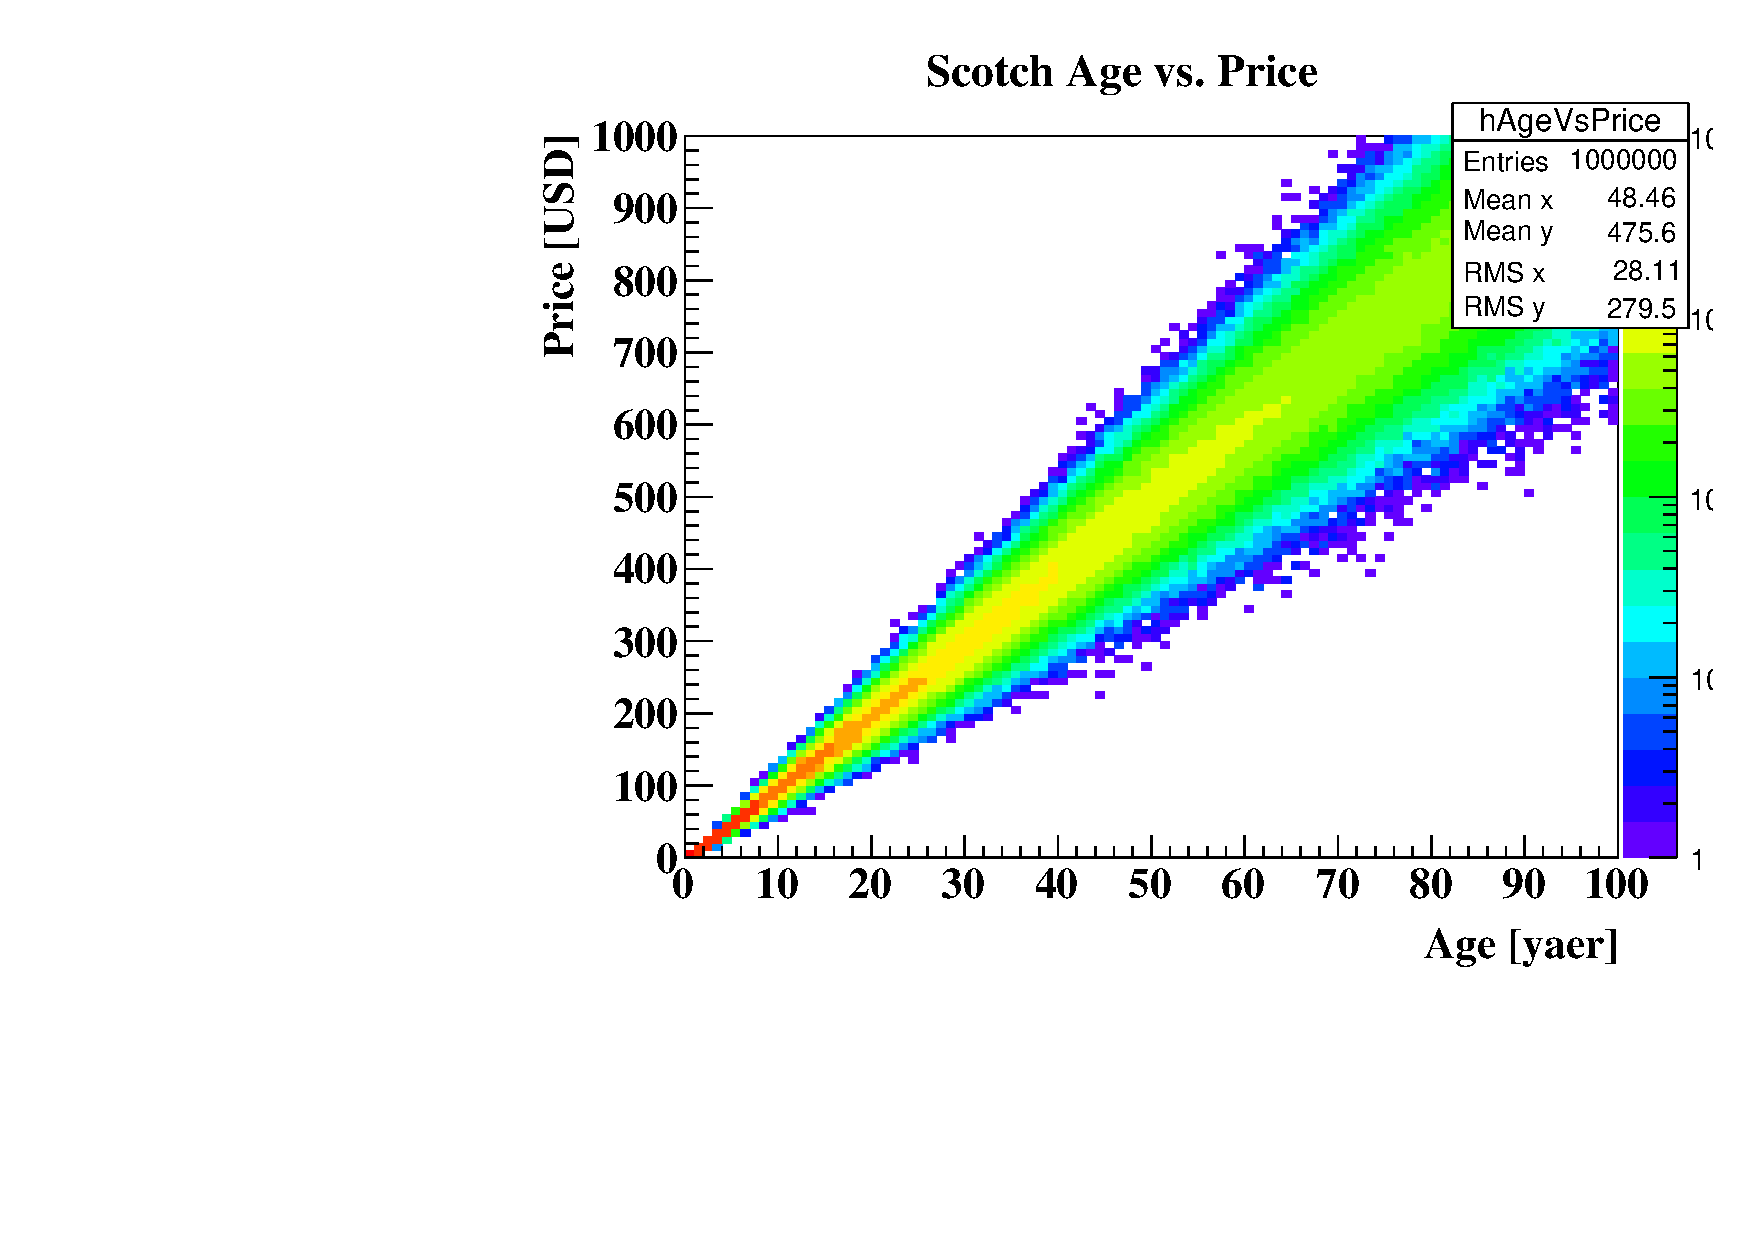
\includegraphics[width=12cm]{./img/ScotchAgeVsPrice.pdf}
\caption{ 
Drawing the age vs. price distribution of {\ttfamily example::Scotch} class from {\ttfamily TTree::Draw}.
}
\end{center}\end{figure}

An example script {\ttfamily mac/example.py} demonstrates how you can:
\begin{itemize}
\item Instantiate {\ttfamily example::Scotch} and save it in a \ROOT file
\item Create a {\ttfamily TTree} of {\ttfamily example::Scotch} for 1e6 entries and save
\item Read-in stored {\ttfamily TTree} and make a very simple access to the stored data product
\item Read-in stored {\ttfamily TTree} and call {\ttfamily TTree::Draw} on the stored data product
\end{itemize}

Note that storing multiple variables into a separate branch of {\ttfamily TTree} (i.e. Ntuple approach)
is much more tedious than storing a class instance as demonstrated in {\ttfamily Scotch::ShipScotch}
function. There, you can find a single line to create a {\ttfamily TTree} branch:
\begin{lstlisting}
tree.Branch("scotch",&data);
\end{lstlisting}
where ``data'' is a {\ttfamily example::Scotch} instance.
With this single line call, all variables in {\ttfamily example::Scotch} instance is stored
with a proper type, and will be readout correctly.

Another myth often people have is that it is very hard to access this object information from
{\ttfamily TTree}. As you can see in the {\ttfamily example.py}, this is completely irrelevant:
you can access the object directly via branch name. A single line in {\ttfamily Python} from
the script is shown below:
\begin{lstlisting}
ch.scotch.Speak()
\end{lstlisting}
which accesses the stored object and calling the class member function {\ttfamily example::Beer::Speak()}.

\subsection{Package Dependency}
The package {\ttfamily Example/Dependent} is prepared to demonstrate how one can make an inter-package 
dependency. In particular, this package depends on {\ttfamily Example/Function} package. Make sure
you have finished building {\ttfamily Example/Function} before building this package.

As you can see in {\ttfamily Stout.h}, the \CPP class {\ttfamily example::Stout} inherits from
{\ttfamily example::Beer}. In order to avoid re-compilation of {\ttfamily example::Beer} class,
we take a usual approach of just {\it linking} the libraries together. Take a look at 
{\ttfamily GNUmakefile}, in particular the following lines:
\begin{lstlisting}
...
INCFLAGS += -I$(LARLITE_USERDEVDIR)/Example
...
LDFLAGS += -L$(LARLITE_LIBDIR) -lExample_Function
\end{lstlisting}
As advertised in the previous section, you must include the path to find {\ttfamily Beer.h} (which
is called from {\ttfamily Stout.h} via {\ttfamily \#include ``Beer.h''}) in {\ttfamily INCFLAGS}, and
both a path and name of a library that contains {\ttfamily example::Beer} class definition in
{\ttfamily LDFLAGS}. 

An example script {\ttfamily mac/example.py} demonstrates an instantiation of {\ttfamily example::Stout}
class and also a call to its base class function {\ttfamily example::Beer::Speak()}.

\subsection{\python in \CPP}
Finally, some users are interested in developing \CPP code to directly operate on \python objects.
An example {\ttfamily Example/PyExample} is prepared to give a tip on how one can write a \CPP
API for \python. This is much better documented as a part of \python documentation:
\begin{center}
{\color{blue}\url{https://docs.python.org/2/c-api/}}
\end{center}

Using a native \python \CPP API is not very easy nor straight forward. Hence in this example,
again, we use \PyROOT binding that makes our life much easier. In short, a difference of two
methods is that you do not have to write your own binding, which is an extra code that has nothing
to do with your algorithm. Finally, that being said, there are other bindings available out there
such as {\ttfamily Cython} (... and \PyROOT uses one of them underneath anyways).

\subsubsection{External Dependnecy}
First of all, you will be using native \python classes, hence you will depend on \python.
Accordingly you have to modify {\ttfamily GNUmakefile}, in particular {\ttfamily INCFLAGS} and
{\ttfamily LDFLAGS}. Notice following 2 lines in {\ttfamily GNUmakefile}:
\begin{lstlisting}
...
INCFLAGS += $(shell python-config --includes)
...
LDFLAGS += $(shell python-config --ldflags)
\end{lstlisting}
each specifying an extra path to find a \python header file and libraries.

\subsubsection{Hiding \python Header From \CINT}
\python header file is called {\ttfamily Python.h}, and is not parse-able via \ROOT \CINT
compiler. So you have to hide it from \CINT dictionary generation step. This can be seen
in {\ttfamily PyExample.h} header file:
\begin{lstlisting}
...
#ifndef __CINT__
// You have to hide native Python header include from CINT                                                                                                                                                  
#include "Python.h"
#endif
...
\end{lstlisting}

You also need to provide two magic lines to forward declare types:
\begin{lstlisting}
...
struct _object;
typedef _object PyObject;
...
\end{lstlisting}
which is for \python generic object pointers to be used (this is a part of \python \CPP API).

\subsubsection{{\ttfamily example::PyExample::Convert}}
The example class {\ttfamily example::PyExample} has an example function to create a
\python list from a \CPP {\ttfamily std::vector<std::string>} object. You can look at the
source code as to how one can do this very simple operation, and take a look at \python
documentation for doing more elaborate operations.

Running {\ttfamily mac/example.py} should show you how this function works.
Obviously you may want to expand the code to work with more advanced \python objects
such as {\ttfamily numpy} array, {\ttfamily matplotlib} axis, and such. The author
does not have much experience to extend too far, but is happy to discuss if you need a help.

\subsection{Documenting Code Using {\ttfamily Doxygen}}
Though this is not everyone's favorite choice, {\ttfamily doxygen} is a popular method to
provide an in-line documentation in the source code. It works pretty nicely with \CPP, and
somewhat at acceptable level with \python. It is the recommended choice for LArSoft to provide
a minimal documentation.

LArLite repositories comes with a doxygen script. You can try generating a documentation
in {\ttfamily Example} directory by typing:
\begin{lstlisting}
  > make doxygen
\end{lstlisting}
({\bf you need doxygen installed in your system!}).

\begin{figure}[htb]\begin{center}
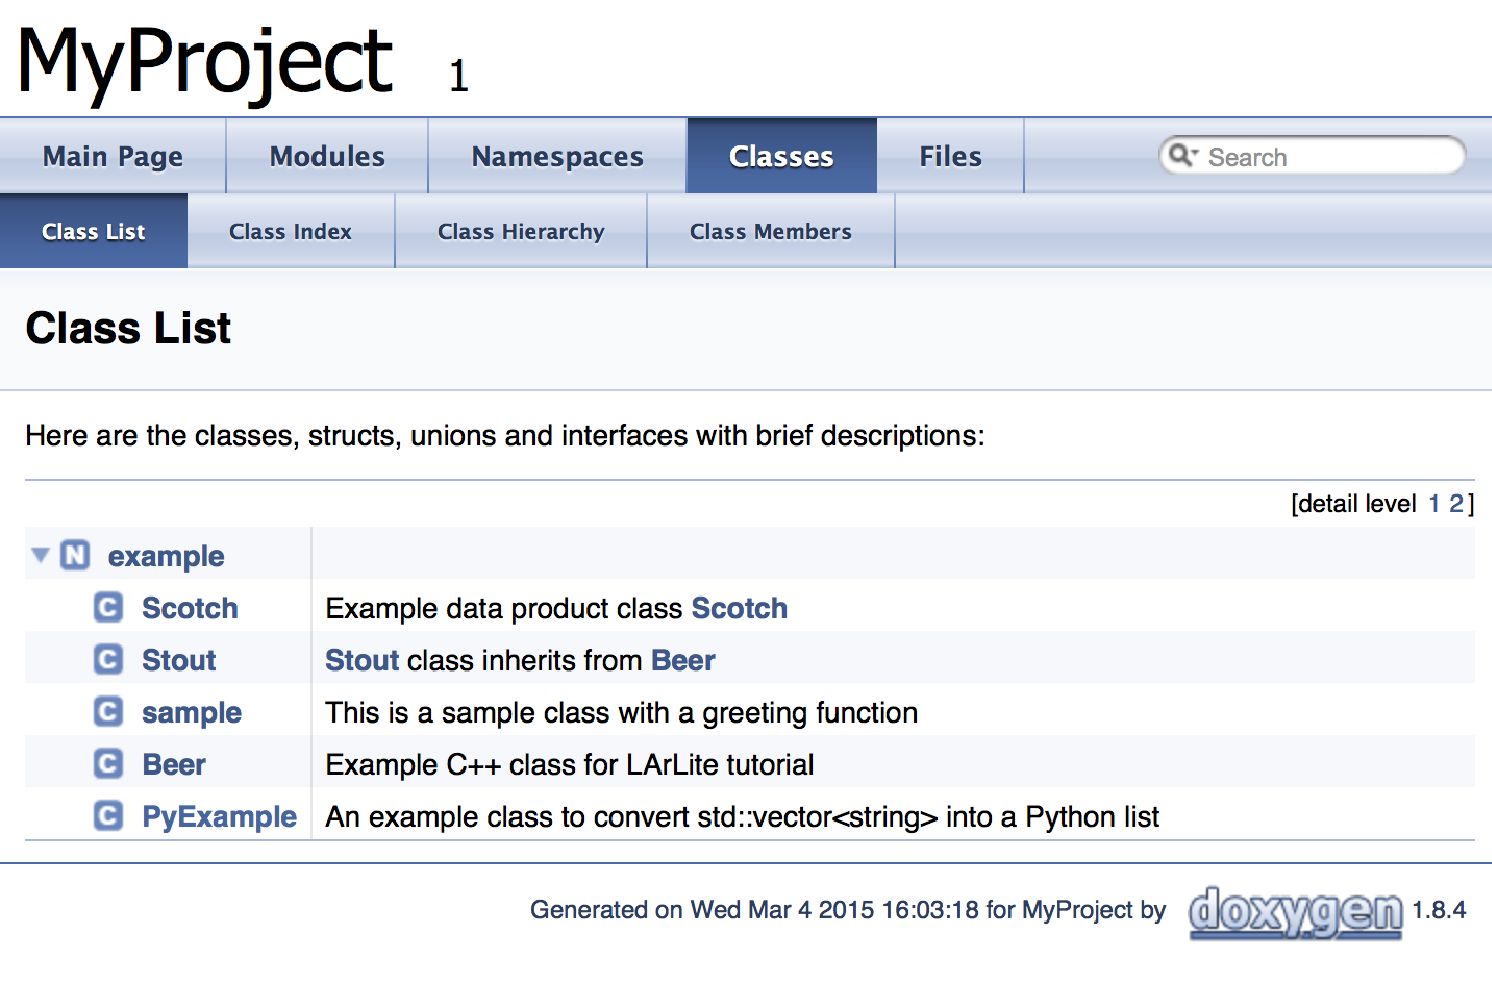
\includegraphics[width=12cm]{./img/doxygen.pdf}
\caption{ 
Doxygen web page generated by ``{\ttfamily make doxygen}'' command for {\ttfamily Example} repository.
}
\end{center}\end{figure}

After successfully running the above command, you should find a chain of HTML files 
to browse through (no internet needed). This way you can also check your doxygen comment
format (whether this is correct or not) before you commit the code. You can look at the
generated documentation using a command like below:
\begin{lstlisting}
  > firefox -a doc/dOxygenMyProject/html/index.html 
\end{lstlisting}
on {\ttfamily Linux} or
\begin{lstlisting}
  > open doc/dOxygenMyProject/html/index.html 
\end{lstlisting}
on {\ttfamily OSX}. The figure shows a generated documentation webpage on the author's laptop.

To understand {\ttfamily doxygen} comment style, refer to their web documentation:
\begin{center}
{\color{blue}\url{http://www.stack.nl/~dimitri/doxygen/manual/docblocks.html}}
\end{center}



% DataFormat package description
\chapter{Core Package: DataFormat}
\label{chap:dataformat}

This chapter discuss about how to generating user's own code development space.
In particular following itmes are discussed in the respective order.
\begin{itemize}
\item Getting started: your own code repository
\item A simple \CPP project package 
\item Stuffing your package
\begin{itemize}
  \item Simple \CPP class
  \item \anaunit (see Ch.\ref{chap:analysis}).
  \item \ertool algorithm class (see \ertool documentation)
  \item \ertool filter class (see \ertool documentation)
  \item \ertool analysis class (see \ertool documentation)
  \item \CPP functions
\end{itemize}
\item Details: LArLite build basics
\item Advanced Code Development
\begin{itemize}
  \item \CPP functions outside classes
  \item Inter-package dependence
  \item Data product: storing \CPP class instance in \ROOT file
  \item \python in \CPP (i.e. opposite of \PyROOT)
\end{itemize}
\end{itemize}

\section{Creating Your Repository}
\label{sec:devrepo}

LArLite supports user code development under \UserDev.
More precisely, it is assumed to be under any path that is set to the value of shell environment variable {\ttfamily \$LARLITE\_USERDEVDIR}. 
For the sake of simplicity we stick with \UserDev in this section.

\subsection{Note About \UserDev}
Important note first:
\begin{itemize}
  \item {\ttfamily UserDev/GNUmakefile}, if it exists, is generated by setup.sh and it does not belong to LArLite repository (ignore it).
  \item Some sub-directories belong to LArLite (see below). Some of these depend on LArLite and some don't. It is useful to note them briefly here.
    \begin{itemize}
        \item {\ttfamily BasicTool} contains useful packages like {\ttfamily GeoAlgo} and has no dependency outside
        \item {\ttfamily SelectionTool} contains useful packages like {\ttfamily ERTool} and depends on {\ttfamily BasicTool}
        \item {\ttfamily RecoTool} contains shower reconstruction code and depends on {\ttfamily core}
        \item {\ttfamily LArLiteApp} contains LArLite application from {\ttfamily GeoAlgo} and {\ttfamily ERTool} 
    \end{itemize}
  \item You can create new directories under \UserDev and that won't bother other users. We'll do this below. 
  This is all done through {\ttfamily .gitignore} rule placed under the top directory. 
\end{itemize}

These features of \UserDev are there so that you feel more free to make a mess (sorry, I meant, to develop code) there!

\subsection{Creating Your Sub-Repository in \UserDev}
\label{sec:devrepo:makenew}
Obviously I cannot just say ``do whatever under \UserDev'' and leave: I would love to support a very easy way to develop code (or make a mess) under \UserDev. I will just show you how to do things here:
\begin{lstlisting}
     > llgen_repository MyRepo
\end{lstlisting}
where the execution command is an alias explained in Sec.\ref{sec:configure}.
This should create a new directory called {\ttfamily MyRepo} under \UserDev. 
That is your new repository. As said, this does not affect LArLite repository. 
If you don't want to keep {\ttfamily MyRepo}, simply ``{\ttfamily rm -r}'' it.

Another thing to note here: your repository will contain code and you will compile them, making a compiled shared object library. 
Your repository name will be used to name your library file (if you follow LArLite code generation scripts described in the followings). 
So pick a name that suits for your purpose. You do not want to pick a generic name that might coincide with some other libraries on your machine.

\subsection{What's in MyRepo?}

Your new repository comes with a GNUmakefile (which does nothing for now) and {\ttfamily doc} 
directory with a doxygen script but empty otherwise. Under this space, you can create your ``packages'' as a 
set of \CPP code to be compiled into a library. We will discuss about more later.

\subsection{Creating Your Sub-Repository in {\ttfamily github}}
In the previous section, we created a new repository {\ttfamily MyRepo} under \UserDev. But that's just a directory on your laptop, and you may want to keep it as your code repository using either {\ttfamily svn} or {\ttfamily github} (or anything else you would like to use). Here, I briefly mention how you can do this using {\ttfamily github} because it's very easy given that you already have a {\ttfamily github} account.

First of all, go to {\ttfamily github.com} and create your own repository: go to your {\ttfamily github} account web page, and click on ``+'' symbol that is toward right-top of the web page. Choose ``New repository''. Then enter the repository name you are about to create. Ideally you may want to choose a somewhat unique name as described in Sec.\ref{sec:devrepo:makenew}. You can always remove your repository if you don't like it.

Then checkout your empty repository. As an example, I use my empty repo called {\ttfamily EmptyRepo}.
\begin{lstlisting}
    > cd $LARLITE_USERDEVDIR
    > git clone git@github.com:drinkingkazu/EmptyRepo EmptyRepo
\end{lstlisting}
Now simply run:
\begin{lstlisting}
    > python bin/gen_new_repository EmptyRepo
    > cd EmptyRepo
    > git add .
    > git commit -m ``new repository''
    > gitpush -u origin master
\end{lstlisting}
and you are done!
From the next time, if you want to install LArLite from scratch, simply checkout your repository under UserDev with the same name.

As said many times, of course, your repository is independent of LArLite repository.





\section{Creating a Package}
\label{sec:package}
Here, I assume we are working under {\ttfamily UserDev/MyRepo}. 
In fact, since it's tedious, I will just refer to {\ttfamily MyRepo}.

\subsection{What is a ``Package''?}
``Package'' is a directory under a repository that is compiled and generates one {\bf shred object library}
(i.e. a file with {\ttfamily .so} extension). This library is loaded at a run-time or linked via compiler as one byte code file.
This gives you a sense of what to include in one package: having too many classes (and especially unrelated classes) in one package
means an extra overhead cost for a run-time loading or linking at compilation. In other words, you probably do not want make one 
library per class, but also not one library for all classes. A package should contain a group of \CPP classes/functions which you
think it makes sense to put together.

\subsection{Making a Simple \CPP Package}

Like advertised many times, LArLite was originally a \CPP project play ground for summer students. 
The author thinks it's very important to have an empty \CPP package generator that comes with build system, 
so that a user can focus on writing the algorithm instead of figuring out how to compile and such.

So here it is: there is a \python script to generate an empty \CPP package:
\begin{lstlisting}
    $LARLITE_BASEDIR/bin/gen_package
\end{lstlisting}
This script takes one input argument which is used to name a ``package'', a directory to be created under {\ttfamily MyRepo}.
This script {\bf needs to be executed somewhere under {\ttfamily MyRepo}} (otherwise you'll see an error message).
One can run this script via alias:
\begin{lstlisting}
    > llgen_package MyProject
\end{lstlisting}
which will create a directory {\ttfamily MyRepo/MyProject} that include minimal set of source codes to compile an empty \CPP class. 
You can have your name choice in place of ``MyProject''. After running the command, try:
\begin{lstlisting}
    > cd MyProject
    > make -j4
\end{lstlisting}
This compiles your code and makes {\ttfamily libMyRepo\_MyProject.so} under {\ttfamily lib} directory.
What you compiled is a \CPP class called ``sample'' defined in {\ttfamily sample.h}. 


\subsection{Using in Interpreter}

So how can you ``use'' this \CPP class? You can write a binary executable code, or try out in \CINT or \PyROOT. Here is an example:
\begin{lstlisting}
    > root
    root[0] sample k;
\end{lstlisting}
Above lines work (i.e. your class instance is created) because \CINT is informed about your class. 

\subsection{``Hello World'' Development}
\label{sec:helloworld}
Let's try a simple modification to your class. Here's an example ``hello world'' program using \CPP class. Open {\ttfamily sample.h} and add a {\ttfamily void} function as shown below:
\begin{lstlisting}
class sample{
public:
  /// Default constructor
  sample(){};
  /// Default destructor
  virtual ~sample(){};
  /// Hello world!
  void HelloWorld() { std::cout << ``Hello World!'' << std::endl; }
};
\end{lstlisting}
Save, close and compile (i.e. type ``make''). Now, try the following in \CINT or \PyROOT:
\begin{lstlisting}
    > root
    root[0] sample k;
    root[1] k.HelloWorld();
    Hello World!
    root[2]
\end{lstlisting}

Whenever you want to start a new project with an empty class, you can come back to this example and create your new \CPP project!





\section{Adding Basic \CPP Classes}
\label{sec:expand_package}

As discussed in the previous section, one should populate a package with a group of \CPP classes.
This section describes how to add various types of \CPP classes to your package.

\subsection{Simple \CPP Class}
Sometimes (rather often) you want to generate a completely generic \CPP class for very good reasons: to develop 
some algorithm that is independent of the framework (= easy portability to outside LArLite).

Here is a script for you:
\begin{lstlisting}
    > cd $LARLITE_USERDEVDIR/MyRepo/MyProject
    > llgen_class_empty MyEmptyClass
\end{lstlisting}
Now you should see {\ttfamily MyEmptyClass.h} and {\ttfamily MyEmptyClass.cxx} created under {\ttfamily MyAna}
package. There also made appropriate modification to {\ttfamily LinkDef.h} so that you can just type:
\begin{lstlisting}
    > make -j2
\end{lstlisting}
to compile your new class. Now develop your awesome algorithm and make it a non-empty class ;)

\subsection{\anaunit Class}
If you wish to generate an empty \anaunit class code (to be implemented by you), simply try:
\begin{lstlisting}
    > cd $LARLITE_USERDEVDIR/MyRepo/MyProject
    > llgen_class_anaunit MyAna
\end{lstlisting}

Executing above commands create {\ttfamily MyAna.cxx} and {\ttfamily MyAna.h} (and an appropriate modification to {\ttfamily LinkDef.h}).
Try:
\begin{lstlisting}
    > make -j4
\end{lstlisting}
You just made your new \anaunit class, {\ttfamily MyAna}, whieh inherits from {\ttfamily ana\_base}! 
Your new \anaunit is accessible from \CINT or \PyROOT like any other classes in LArLite:
\begin{lstlisting}
    > root
    root[0] larlite::MyAna my_ana_instance
\end{lstlisting}
Now go ahead and code up this analysis unit, and run with {\ttfamily ana\_processor}! 

\subsubsection{Run Your Analysis Unit: \PyROOT}
\label{sec:yourrunscript}
There is an example \python run script for \anaunit under {\ttfamily mac} directory, called 
{\ttfamily example\_anaunit.py}. You need a LArLite sample \ROOT file to run this program. 
If you have a sample file, say {\ttfamily trial.root}, you can run the program as follows.
\begin{lstlisting}
    > python mac/example_anaunit.py trial.root
\end{lstlisting}

\subsection{\ertool Classes}
Just as we exercised how to add a new \CPP class to a package, there's analogous python scripts to
generate \ertool reconstruction algorithm, filter, and analysis class:
\begin{lstlisting}
    > cd $LARLITE_USERDEVDIR/MyRepo/MyProject
    > llgen_class_erfilter Trial
    > llgen_class_eralgo Trial
    > llgen_class_erana Trial
\end{lstlisting}
Above three commands generate three \CPP classes: {\ttfamily ERFilterTrial}, {\ttfamily ERAlgoTrial}, and {\ttfamily ERAnaTrial}.
These are implementation of base classes defined in \ertool, hence must be used with {\ttfamily ertool::Manager}.
For details, see \ertool documentation (which is to come...)






\section{Understanding the Build}
\label{sec:build_package}
This section covers the basics of how the LArLite build works, aiming to reduce a black-box content for users and developers.
The following topics are ordered such that a topic of interest to more people gets covered first.

\subsection{{\ttfamily Compiler} and {\ttfamily Linker} for Dummies}
Skip if you already know about them, obviously.

Our \CPP source codes are merely descriptions of what we want our computer to do in human-friendly language 
(disagree on ``human-fiendly''? Welcome to the club).
A {\ttfamily compiler} takes in our source code and generate a machine-friendly description, often called as an {\it object file} or {\it byte code}.
When you compile your package in LArLite, you find files with {\ttfamily .o} extension: these are the object files.

Now having many granular object files is not very helpful.
A {\ttfamily linker} allows us to combine multiple object files and create a {\it shared object library} file.
You find such files with {\ttfamily .so} extension under {\ttfamily \$LARLITE\_LIBDIR} if you compiled any package.
The scope of what objects should be put together is really a developer's choice.
In LArLite, this is done per package.
Another (and more important) advantage of shared object libraries kicks in when you compile another code that depends on it.
Say you have a \CPP class {\ttfamily A} and {\ttfamily B} where {\ttfamily B} depends on {\ttfamily A}. 
Once you have {\ttfamily A} compiled with {\ttfamily .so} file, a separate compilation of {\ttfamily B} does not require
a re-compilation of {\ttfamily A}'s source code. Instead, you can {\it link} the {\ttfamily A}'s library upon compilation
of {\ttfamily B}'s library.

In LArLite, we compile files with {\ttfamily .cxx} extensions with a compiler, and create a shared object library using a linker, which
is nothing special compared to any other softwares' build system.

\subsection{{\ttfamily INCFLAGS} and {\ttfamily LDFLAGS}: LArLite Compiler Flags}
In LArLite package's {\ttfamily GNUmakefile}, you may see variables named as {\ttfamily INCFLAGS} and {\ttfamily LDFLAGS} where
the latter may not appear in some simple code packages (i.e. don't worry about not seeing {\ttfamily LDFLAGS} in your {\ttfamily GNUmakefile}).
These are called {\it compiler flags} and passed onto a compiler and linker respectively.

\subsubsection{INCFLAGS}
{\ttfamily INCFLAGS} is used by a compiler to search for files you specify with {\ttfamily \#include} preprocessor command in your source code.
In other words, if your source code calls {\ttfamily \#include <TH1D.h>}, then the directory path which contains {\ttfamily TH1D.h} has to be
added to {\ttfamily INCFLAGS}. The format of {\ttfamily INCFLAGS} is ``-I\$PATH'' where you should replace ``\$PATH'' with the relevant
directory path.

That being said, by default, LArLite includes a \ROOT's include flags.
\ROOT follows a standard method to provide such flags, and you can try this in your installation as well:
\begin{lstlisting}
  > root-config --cflags
\end{lstlisting}
The output of above command is a part of LArLite's default {\ttfamily INCFLAGS}.

\subsubsection{LDFLAGS}
{\ttfamily LDFLAGS} is used by a linker to find libraries to be linked into your package. If your package depends on any externaly compiled
code, for instance a \ROOT class {\ttfamily TH1D}, you have to specify the library to be linked here. The format is 
{\ttfamily -L\$PATH -l\$LIBNAME} where ``\$PATH'' is the directory path that contains a library named ``lib\$LIBNAME.so''. Note that
you should exclude the prefix ``lib'' when you specify it in {\ttfamily LDFLAGS} as that is the standard of how a linker takes in library names.

The default flags in LArLite includes a \ROOT's library flags.
Again, as it was the case for {\ttfamily INCFLAGS}, you can try:
\begin{lstlisting}
  > root-config --libs
\end{lstlisting}
which include most of standard \ROOT libraries such as IO, histogram, TTree, TMatrix, TVector3, etc.

\subsubsection{Flags for LArLite Packages}
You may write a package that depends on existing LArLite code.
One example is an analysis code that inherits from {\ttfamily lalrite::ana\_base}. 
Then you will have to specify {\ttfamily INCFLAGS} and {\ttfamily LDFLAGS}.

Specifying every single {\ttfamily INCFLAGS} and {\ttfamily LDFLAGS} for LArLite code is definitely annoying.
So we follow the popular standard and the following scripts are prepared:
\begin{itemize}
\item {\ttfamily larlite-config} for LArLite's analysis framework
\item {\ttfamily basictool-config} for code under \UserDev/BasicTool 
\item {\ttfamily seltool-config} for code under \UserDev/SelectionTool
\item {\ttfamily recotool-config} for code under \UserDev/RecoTool
\end{itemize}
These scripts can be run with either {\ttfamily --includes} or {\ttfamily --libs} option, and they
simply prints out relevant string to be added to {\ttfamily INCFLAGS} and {\ttfamily LDFLAGS} respectively.
For instance, you may try:
\begin{lstlisting}
  INCFLAGS += $(shell larlite-config --includes)
\end{lstlisting}
and/or
\begin{lstlisting}
  LDFLAGS += $(shell larlite-config --libs)
\end{lstlisting}
in your {\ttfamily GNUmakefile}.

If you use {\ttfamily gen\_class\_anaunit} or similar script, actually, this modification to a {\ttfamily GNUmakefile} is done
by the same script. Hence you do not need to worry about it.

\subsection{Compiler \& Linker Used by LArLite}
Let me make a brief note on how compiler/linker is picked and what default compiler/linker flags are set for LArLite build.

When possible LArLite attempts to use \clang++. In particular this is searched and set when one runs {\ttfamily setup.sh} script.
The configured compiler name is set to a shell environment variable {\ttfamily \$LARLITE\_CXX}.
Further, compiler/linker specific flags are defined in:
\begin{lstlisting}
  > $LARLITE_BASEDIR/Makefile/Makefile.X
\end{lstlisting}
where {\ttfamily X} may be either ``Darwin'' or ``Linux''. 


\section{Advanced Development}
\label{sec:advanced_package}

In this section we follow a prepared example that can be found in:
\begin{center}
{\color{blue}\url{https://github.com/drinkingkazu/Example}}
\end{center}
You might have already checked out this repository as this was mentioned briefly
in the introductory section (see Sec.\ref{sec:build}). 
If not, can certainly checkout under \UserDev:
\begin{lstlisting}
  > cd $LARLITE_USERDEVDIR
  > git clone https://github.com/drinkingkazu/Example
\end{lstlisting}

This repository contains following packages:
\begin{itemize}
\item {\ttfamily Empty} for the simplest example to introduce a simple \CPP class
\item {\ttfamily Function} for demonstrating a \CPP function to be exported into a dictionary
\item {\ttfamily Dependent} for showing how to make inter-package dependencies
\item {\ttfamily DataProduct} as an example of how to store a class instance into a file
\end{itemize}
where we skip the first item, {\ttfamily Empty}, as that has been covered in the previous section.

\subsection{\CPP Functions}
I would like to avoid a confusion: \CPP class is an extension of data structure. In particular,
you do not have to make \CPP class for inventing one or a few functions. Just like we have done
some practice with \CPP class, it would be useful to have \CPP functions in a dictionary.
The point of this package is to show how one can do this.

Take a look at {\ttfamily MyFunctions.h} and {\ttfamily MyFunctions.cxx} source code: there, I defined
functions:
\begin{lstlisting}
  void hello_world();
  Beer Brew(const int age);
\end{lstlisting}
where {\ttfamily example::Beer} is a \CPP class defined in {\ttfamily Beer.h}: it's very very simple class for
playing around unlike the sophisticated name.

Now a compilation works just as expected, and there is nothing special about these functions.
What you may find useful is a format to declare above functions in {\ttfamily LinkDef.h}:
\begin{lstlisting}
#pragma link C++ function  example::hello_world()+;
#pragma link C++ function  example::Brew(const int)+;
\end{lstlisting}
As you can see, a) you do not specify the return type of the function, and b) you only need to specify
the argument types. 

You can try executing an example script {\ttfamily mac/example.py} which calls those functions. 
Take a look at the script's contents and see if that makes sense (... and ask a question if you have any!).
{\color{red}\bf There is one caveat}, however: currently \ROOT seems to require \CPP class compiled
in the same library to be instantiated {\bf before} \CPP functions to be called. The author will
open a ticket for this to be fixed.

\subsection{\ROOT Data Product Class}
Once you get familiar with all LArLite features, you might want to store \CPP object in a file
as a {\ttfamily data product}. The easiest (and recommended) method is to use a \ROOT file.
A rule of the thumb is that any \CPP class that is generated with a \ROOT {\it dictionary} can
be stored in a \ROOT file. You can find details in the \ROOT manual.

If you use LArLite as your code development environment, \ROOT dictionary file is always
generated and built at compilation stage of your package. 

An example can be found in the package {\ttfamily DataProduct}.
There, a data product class called {\ttfamily example::Scotch} is defined. 

\begin{figure}[htb]\begin{center}
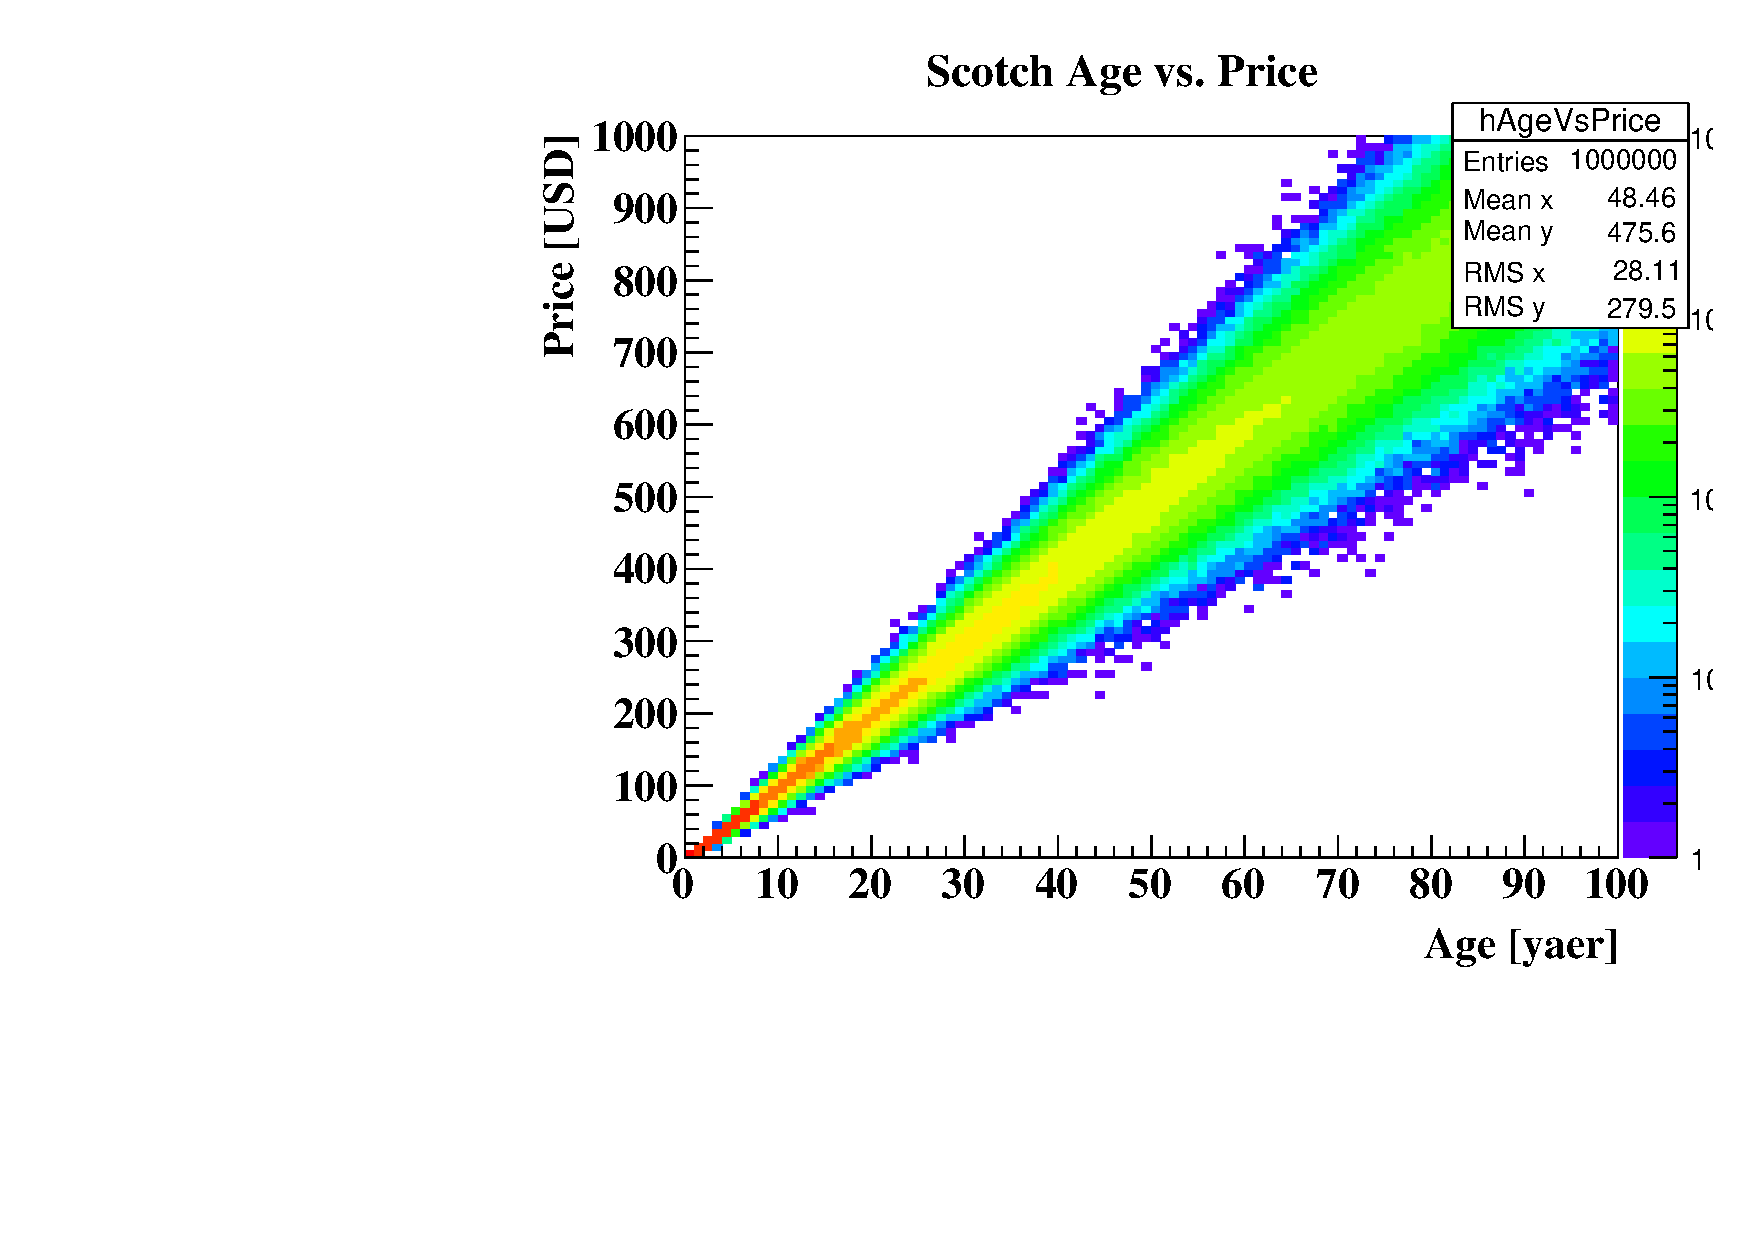
\includegraphics[width=12cm]{./img/ScotchAgeVsPrice.pdf}
\caption{ 
Drawing the age vs. price distribution of {\ttfamily example::Scotch} class from {\ttfamily TTree::Draw}.
}
\end{center}\end{figure}

An example script {\ttfamily mac/example.py} demonstrates how you can:
\begin{itemize}
\item Instantiate {\ttfamily example::Scotch} and save it in a \ROOT file
\item Create a {\ttfamily TTree} of {\ttfamily example::Scotch} for 1e6 entries and save
\item Read-in stored {\ttfamily TTree} and make a very simple access to the stored data product
\item Read-in stored {\ttfamily TTree} and call {\ttfamily TTree::Draw} on the stored data product
\end{itemize}

Note that storing multiple variables into a separate branch of {\ttfamily TTree} (i.e. Ntuple approach)
is much more tedious than storing a class instance as demonstrated in {\ttfamily Scotch::ShipScotch}
function. There, you can find a single line to create a {\ttfamily TTree} branch:
\begin{lstlisting}
tree.Branch("scotch",&data);
\end{lstlisting}
where ``data'' is a {\ttfamily example::Scotch} instance.
With this single line call, all variables in {\ttfamily example::Scotch} instance is stored
with a proper type, and will be readout correctly.

Another myth often people have is that it is very hard to access this object information from
{\ttfamily TTree}. As you can see in the {\ttfamily example.py}, this is completely irrelevant:
you can access the object directly via branch name. A single line in {\ttfamily Python} from
the script is shown below:
\begin{lstlisting}
ch.scotch.Speak()
\end{lstlisting}
which accesses the stored object and calling the class member function {\ttfamily example::Beer::Speak()}.

\subsection{Package Dependency}
The package {\ttfamily Example/Dependent} is prepared to demonstrate how one can make an inter-package 
dependency. In particular, this package depends on {\ttfamily Example/Function} package. Make sure
you have finished building {\ttfamily Example/Function} before building this package.

As you can see in {\ttfamily Stout.h}, the \CPP class {\ttfamily example::Stout} inherits from
{\ttfamily example::Beer}. In order to avoid re-compilation of {\ttfamily example::Beer} class,
we take a usual approach of just {\it linking} the libraries together. Take a look at 
{\ttfamily GNUmakefile}, in particular the following lines:
\begin{lstlisting}
...
INCFLAGS += -I$(LARLITE_USERDEVDIR)/Example
...
LDFLAGS += -L$(LARLITE_LIBDIR) -lExample_Function
\end{lstlisting}
As advertised in the previous section, you must include the path to find {\ttfamily Beer.h} (which
is called from {\ttfamily Stout.h} via {\ttfamily \#include ``Beer.h''}) in {\ttfamily INCFLAGS}, and
both a path and name of a library that contains {\ttfamily example::Beer} class definition in
{\ttfamily LDFLAGS}. 

An example script {\ttfamily mac/example.py} demonstrates an instantiation of {\ttfamily example::Stout}
class and also a call to its base class function {\ttfamily example::Beer::Speak()}.

\subsection{\python in \CPP}
Finally, some users are interested in developing \CPP code to directly operate on \python objects.
An example {\ttfamily Example/PyExample} is prepared to give a tip on how one can write a \CPP
API for \python. This is much better documented as a part of \python documentation:
\begin{center}
{\color{blue}\url{https://docs.python.org/2/c-api/}}
\end{center}

Using a native \python \CPP API is not very easy nor straight forward. Hence in this example,
again, we use \PyROOT binding that makes our life much easier. In short, a difference of two
methods is that you do not have to write your own binding, which is an extra code that has nothing
to do with your algorithm. Finally, that being said, there are other bindings available out there
such as {\ttfamily Cython} (... and \PyROOT uses one of them underneath anyways).

\subsubsection{External Dependnecy}
First of all, you will be using native \python classes, hence you will depend on \python.
Accordingly you have to modify {\ttfamily GNUmakefile}, in particular {\ttfamily INCFLAGS} and
{\ttfamily LDFLAGS}. Notice following 2 lines in {\ttfamily GNUmakefile}:
\begin{lstlisting}
...
INCFLAGS += $(shell python-config --includes)
...
LDFLAGS += $(shell python-config --ldflags)
\end{lstlisting}
each specifying an extra path to find a \python header file and libraries.

\subsubsection{Hiding \python Header From \CINT}
\python header file is called {\ttfamily Python.h}, and is not parse-able via \ROOT \CINT
compiler. So you have to hide it from \CINT dictionary generation step. This can be seen
in {\ttfamily PyExample.h} header file:
\begin{lstlisting}
...
#ifndef __CINT__
// You have to hide native Python header include from CINT                                                                                                                                                  
#include "Python.h"
#endif
...
\end{lstlisting}

You also need to provide two magic lines to forward declare types:
\begin{lstlisting}
...
struct _object;
typedef _object PyObject;
...
\end{lstlisting}
which is for \python generic object pointers to be used (this is a part of \python \CPP API).

\subsubsection{{\ttfamily example::PyExample::Convert}}
The example class {\ttfamily example::PyExample} has an example function to create a
\python list from a \CPP {\ttfamily std::vector<std::string>} object. You can look at the
source code as to how one can do this very simple operation, and take a look at \python
documentation for doing more elaborate operations.

Running {\ttfamily mac/example.py} should show you how this function works.
Obviously you may want to expand the code to work with more advanced \python objects
such as {\ttfamily numpy} array, {\ttfamily matplotlib} axis, and such. The author
does not have much experience to extend too far, but is happy to discuss if you need a help.

\subsection{Documenting Code Using {\ttfamily Doxygen}}
Though this is not everyone's favorite choice, {\ttfamily doxygen} is a popular method to
provide an in-line documentation in the source code. It works pretty nicely with \CPP, and
somewhat at acceptable level with \python. It is the recommended choice for LArSoft to provide
a minimal documentation.

LArLite repositories comes with a doxygen script. You can try generating a documentation
in {\ttfamily Example} directory by typing:
\begin{lstlisting}
  > make doxygen
\end{lstlisting}
({\bf you need doxygen installed in your system!}).

\begin{figure}[htb]\begin{center}
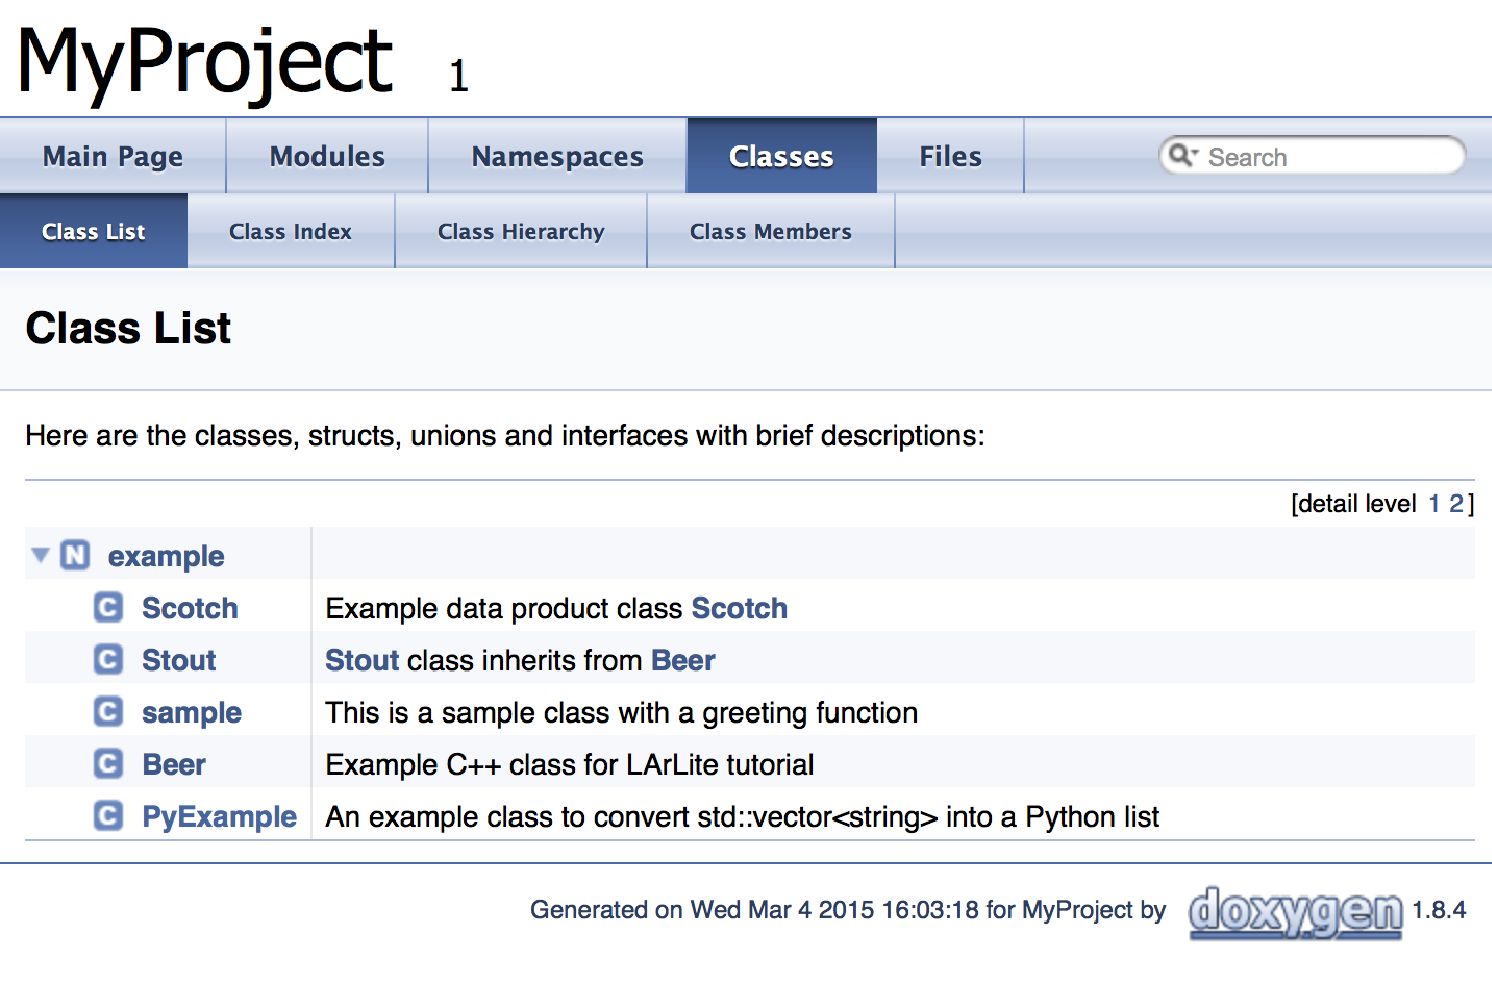
\includegraphics[width=12cm]{./img/doxygen.pdf}
\caption{ 
Doxygen web page generated by ``{\ttfamily make doxygen}'' command for {\ttfamily Example} repository.
}
\end{center}\end{figure}

After successfully running the above command, you should find a chain of HTML files 
to browse through (no internet needed). This way you can also check your doxygen comment
format (whether this is correct or not) before you commit the code. You can look at the
generated documentation using a command like below:
\begin{lstlisting}
  > firefox -a doc/dOxygenMyProject/html/index.html 
\end{lstlisting}
on {\ttfamily Linux} or
\begin{lstlisting}
  > open doc/dOxygenMyProject/html/index.html 
\end{lstlisting}
on {\ttfamily OSX}. The figure shows a generated documentation webpage on the author's laptop.

To understand {\ttfamily doxygen} comment style, refer to their web documentation:
\begin{center}
{\color{blue}\url{http://www.stack.nl/~dimitri/doxygen/manual/docblocks.html}}
\end{center}



% Analysis package description
\chapter{Core Package: Analysis}
\label{chap:analysis}

This chapter discuss about how to generating user's own code development space.
In particular following itmes are discussed in the respective order.
\begin{itemize}
\item Getting started: your own code repository
\item A simple \CPP project package 
\item Stuffing your package
\begin{itemize}
  \item Simple \CPP class
  \item \anaunit (see Ch.\ref{chap:analysis}).
  \item \ertool algorithm class (see \ertool documentation)
  \item \ertool filter class (see \ertool documentation)
  \item \ertool analysis class (see \ertool documentation)
  \item \CPP functions
\end{itemize}
\item Details: LArLite build basics
\item Advanced Code Development
\begin{itemize}
  \item \CPP functions outside classes
  \item Inter-package dependence
  \item Data product: storing \CPP class instance in \ROOT file
  \item \python in \CPP (i.e. opposite of \PyROOT)
\end{itemize}
\end{itemize}

\section{Creating Your Repository}
\label{sec:devrepo}

LArLite supports user code development under \UserDev.
More precisely, it is assumed to be under any path that is set to the value of shell environment variable {\ttfamily \$LARLITE\_USERDEVDIR}. 
For the sake of simplicity we stick with \UserDev in this section.

\subsection{Note About \UserDev}
Important note first:
\begin{itemize}
  \item {\ttfamily UserDev/GNUmakefile}, if it exists, is generated by setup.sh and it does not belong to LArLite repository (ignore it).
  \item Some sub-directories belong to LArLite (see below). Some of these depend on LArLite and some don't. It is useful to note them briefly here.
    \begin{itemize}
        \item {\ttfamily BasicTool} contains useful packages like {\ttfamily GeoAlgo} and has no dependency outside
        \item {\ttfamily SelectionTool} contains useful packages like {\ttfamily ERTool} and depends on {\ttfamily BasicTool}
        \item {\ttfamily RecoTool} contains shower reconstruction code and depends on {\ttfamily core}
        \item {\ttfamily LArLiteApp} contains LArLite application from {\ttfamily GeoAlgo} and {\ttfamily ERTool} 
    \end{itemize}
  \item You can create new directories under \UserDev and that won't bother other users. We'll do this below. 
  This is all done through {\ttfamily .gitignore} rule placed under the top directory. 
\end{itemize}

These features of \UserDev are there so that you feel more free to make a mess (sorry, I meant, to develop code) there!

\subsection{Creating Your Sub-Repository in \UserDev}
\label{sec:devrepo:makenew}
Obviously I cannot just say ``do whatever under \UserDev'' and leave: I would love to support a very easy way to develop code (or make a mess) under \UserDev. I will just show you how to do things here:
\begin{lstlisting}
     > llgen_repository MyRepo
\end{lstlisting}
where the execution command is an alias explained in Sec.\ref{sec:configure}.
This should create a new directory called {\ttfamily MyRepo} under \UserDev. 
That is your new repository. As said, this does not affect LArLite repository. 
If you don't want to keep {\ttfamily MyRepo}, simply ``{\ttfamily rm -r}'' it.

Another thing to note here: your repository will contain code and you will compile them, making a compiled shared object library. 
Your repository name will be used to name your library file (if you follow LArLite code generation scripts described in the followings). 
So pick a name that suits for your purpose. You do not want to pick a generic name that might coincide with some other libraries on your machine.

\subsection{What's in MyRepo?}

Your new repository comes with a GNUmakefile (which does nothing for now) and {\ttfamily doc} 
directory with a doxygen script but empty otherwise. Under this space, you can create your ``packages'' as a 
set of \CPP code to be compiled into a library. We will discuss about more later.

\subsection{Creating Your Sub-Repository in {\ttfamily github}}
In the previous section, we created a new repository {\ttfamily MyRepo} under \UserDev. But that's just a directory on your laptop, and you may want to keep it as your code repository using either {\ttfamily svn} or {\ttfamily github} (or anything else you would like to use). Here, I briefly mention how you can do this using {\ttfamily github} because it's very easy given that you already have a {\ttfamily github} account.

First of all, go to {\ttfamily github.com} and create your own repository: go to your {\ttfamily github} account web page, and click on ``+'' symbol that is toward right-top of the web page. Choose ``New repository''. Then enter the repository name you are about to create. Ideally you may want to choose a somewhat unique name as described in Sec.\ref{sec:devrepo:makenew}. You can always remove your repository if you don't like it.

Then checkout your empty repository. As an example, I use my empty repo called {\ttfamily EmptyRepo}.
\begin{lstlisting}
    > cd $LARLITE_USERDEVDIR
    > git clone git@github.com:drinkingkazu/EmptyRepo EmptyRepo
\end{lstlisting}
Now simply run:
\begin{lstlisting}
    > python bin/gen_new_repository EmptyRepo
    > cd EmptyRepo
    > git add .
    > git commit -m ``new repository''
    > gitpush -u origin master
\end{lstlisting}
and you are done!
From the next time, if you want to install LArLite from scratch, simply checkout your repository under UserDev with the same name.

As said many times, of course, your repository is independent of LArLite repository.





\section{Creating a Package}
\label{sec:package}
Here, I assume we are working under {\ttfamily UserDev/MyRepo}. 
In fact, since it's tedious, I will just refer to {\ttfamily MyRepo}.

\subsection{What is a ``Package''?}
``Package'' is a directory under a repository that is compiled and generates one {\bf shred object library}
(i.e. a file with {\ttfamily .so} extension). This library is loaded at a run-time or linked via compiler as one byte code file.
This gives you a sense of what to include in one package: having too many classes (and especially unrelated classes) in one package
means an extra overhead cost for a run-time loading or linking at compilation. In other words, you probably do not want make one 
library per class, but also not one library for all classes. A package should contain a group of \CPP classes/functions which you
think it makes sense to put together.

\subsection{Making a Simple \CPP Package}

Like advertised many times, LArLite was originally a \CPP project play ground for summer students. 
The author thinks it's very important to have an empty \CPP package generator that comes with build system, 
so that a user can focus on writing the algorithm instead of figuring out how to compile and such.

So here it is: there is a \python script to generate an empty \CPP package:
\begin{lstlisting}
    $LARLITE_BASEDIR/bin/gen_package
\end{lstlisting}
This script takes one input argument which is used to name a ``package'', a directory to be created under {\ttfamily MyRepo}.
This script {\bf needs to be executed somewhere under {\ttfamily MyRepo}} (otherwise you'll see an error message).
One can run this script via alias:
\begin{lstlisting}
    > llgen_package MyProject
\end{lstlisting}
which will create a directory {\ttfamily MyRepo/MyProject} that include minimal set of source codes to compile an empty \CPP class. 
You can have your name choice in place of ``MyProject''. After running the command, try:
\begin{lstlisting}
    > cd MyProject
    > make -j4
\end{lstlisting}
This compiles your code and makes {\ttfamily libMyRepo\_MyProject.so} under {\ttfamily lib} directory.
What you compiled is a \CPP class called ``sample'' defined in {\ttfamily sample.h}. 


\subsection{Using in Interpreter}

So how can you ``use'' this \CPP class? You can write a binary executable code, or try out in \CINT or \PyROOT. Here is an example:
\begin{lstlisting}
    > root
    root[0] sample k;
\end{lstlisting}
Above lines work (i.e. your class instance is created) because \CINT is informed about your class. 

\subsection{``Hello World'' Development}
\label{sec:helloworld}
Let's try a simple modification to your class. Here's an example ``hello world'' program using \CPP class. Open {\ttfamily sample.h} and add a {\ttfamily void} function as shown below:
\begin{lstlisting}
class sample{
public:
  /// Default constructor
  sample(){};
  /// Default destructor
  virtual ~sample(){};
  /// Hello world!
  void HelloWorld() { std::cout << ``Hello World!'' << std::endl; }
};
\end{lstlisting}
Save, close and compile (i.e. type ``make''). Now, try the following in \CINT or \PyROOT:
\begin{lstlisting}
    > root
    root[0] sample k;
    root[1] k.HelloWorld();
    Hello World!
    root[2]
\end{lstlisting}

Whenever you want to start a new project with an empty class, you can come back to this example and create your new \CPP project!





\section{Adding Basic \CPP Classes}
\label{sec:expand_package}

As discussed in the previous section, one should populate a package with a group of \CPP classes.
This section describes how to add various types of \CPP classes to your package.

\subsection{Simple \CPP Class}
Sometimes (rather often) you want to generate a completely generic \CPP class for very good reasons: to develop 
some algorithm that is independent of the framework (= easy portability to outside LArLite).

Here is a script for you:
\begin{lstlisting}
    > cd $LARLITE_USERDEVDIR/MyRepo/MyProject
    > llgen_class_empty MyEmptyClass
\end{lstlisting}
Now you should see {\ttfamily MyEmptyClass.h} and {\ttfamily MyEmptyClass.cxx} created under {\ttfamily MyAna}
package. There also made appropriate modification to {\ttfamily LinkDef.h} so that you can just type:
\begin{lstlisting}
    > make -j2
\end{lstlisting}
to compile your new class. Now develop your awesome algorithm and make it a non-empty class ;)

\subsection{\anaunit Class}
If you wish to generate an empty \anaunit class code (to be implemented by you), simply try:
\begin{lstlisting}
    > cd $LARLITE_USERDEVDIR/MyRepo/MyProject
    > llgen_class_anaunit MyAna
\end{lstlisting}

Executing above commands create {\ttfamily MyAna.cxx} and {\ttfamily MyAna.h} (and an appropriate modification to {\ttfamily LinkDef.h}).
Try:
\begin{lstlisting}
    > make -j4
\end{lstlisting}
You just made your new \anaunit class, {\ttfamily MyAna}, whieh inherits from {\ttfamily ana\_base}! 
Your new \anaunit is accessible from \CINT or \PyROOT like any other classes in LArLite:
\begin{lstlisting}
    > root
    root[0] larlite::MyAna my_ana_instance
\end{lstlisting}
Now go ahead and code up this analysis unit, and run with {\ttfamily ana\_processor}! 

\subsubsection{Run Your Analysis Unit: \PyROOT}
\label{sec:yourrunscript}
There is an example \python run script for \anaunit under {\ttfamily mac} directory, called 
{\ttfamily example\_anaunit.py}. You need a LArLite sample \ROOT file to run this program. 
If you have a sample file, say {\ttfamily trial.root}, you can run the program as follows.
\begin{lstlisting}
    > python mac/example_anaunit.py trial.root
\end{lstlisting}

\subsection{\ertool Classes}
Just as we exercised how to add a new \CPP class to a package, there's analogous python scripts to
generate \ertool reconstruction algorithm, filter, and analysis class:
\begin{lstlisting}
    > cd $LARLITE_USERDEVDIR/MyRepo/MyProject
    > llgen_class_erfilter Trial
    > llgen_class_eralgo Trial
    > llgen_class_erana Trial
\end{lstlisting}
Above three commands generate three \CPP classes: {\ttfamily ERFilterTrial}, {\ttfamily ERAlgoTrial}, and {\ttfamily ERAnaTrial}.
These are implementation of base classes defined in \ertool, hence must be used with {\ttfamily ertool::Manager}.
For details, see \ertool documentation (which is to come...)






\section{Understanding the Build}
\label{sec:build_package}
This section covers the basics of how the LArLite build works, aiming to reduce a black-box content for users and developers.
The following topics are ordered such that a topic of interest to more people gets covered first.

\subsection{{\ttfamily Compiler} and {\ttfamily Linker} for Dummies}
Skip if you already know about them, obviously.

Our \CPP source codes are merely descriptions of what we want our computer to do in human-friendly language 
(disagree on ``human-fiendly''? Welcome to the club).
A {\ttfamily compiler} takes in our source code and generate a machine-friendly description, often called as an {\it object file} or {\it byte code}.
When you compile your package in LArLite, you find files with {\ttfamily .o} extension: these are the object files.

Now having many granular object files is not very helpful.
A {\ttfamily linker} allows us to combine multiple object files and create a {\it shared object library} file.
You find such files with {\ttfamily .so} extension under {\ttfamily \$LARLITE\_LIBDIR} if you compiled any package.
The scope of what objects should be put together is really a developer's choice.
In LArLite, this is done per package.
Another (and more important) advantage of shared object libraries kicks in when you compile another code that depends on it.
Say you have a \CPP class {\ttfamily A} and {\ttfamily B} where {\ttfamily B} depends on {\ttfamily A}. 
Once you have {\ttfamily A} compiled with {\ttfamily .so} file, a separate compilation of {\ttfamily B} does not require
a re-compilation of {\ttfamily A}'s source code. Instead, you can {\it link} the {\ttfamily A}'s library upon compilation
of {\ttfamily B}'s library.

In LArLite, we compile files with {\ttfamily .cxx} extensions with a compiler, and create a shared object library using a linker, which
is nothing special compared to any other softwares' build system.

\subsection{{\ttfamily INCFLAGS} and {\ttfamily LDFLAGS}: LArLite Compiler Flags}
In LArLite package's {\ttfamily GNUmakefile}, you may see variables named as {\ttfamily INCFLAGS} and {\ttfamily LDFLAGS} where
the latter may not appear in some simple code packages (i.e. don't worry about not seeing {\ttfamily LDFLAGS} in your {\ttfamily GNUmakefile}).
These are called {\it compiler flags} and passed onto a compiler and linker respectively.

\subsubsection{INCFLAGS}
{\ttfamily INCFLAGS} is used by a compiler to search for files you specify with {\ttfamily \#include} preprocessor command in your source code.
In other words, if your source code calls {\ttfamily \#include <TH1D.h>}, then the directory path which contains {\ttfamily TH1D.h} has to be
added to {\ttfamily INCFLAGS}. The format of {\ttfamily INCFLAGS} is ``-I\$PATH'' where you should replace ``\$PATH'' with the relevant
directory path.

That being said, by default, LArLite includes a \ROOT's include flags.
\ROOT follows a standard method to provide such flags, and you can try this in your installation as well:
\begin{lstlisting}
  > root-config --cflags
\end{lstlisting}
The output of above command is a part of LArLite's default {\ttfamily INCFLAGS}.

\subsubsection{LDFLAGS}
{\ttfamily LDFLAGS} is used by a linker to find libraries to be linked into your package. If your package depends on any externaly compiled
code, for instance a \ROOT class {\ttfamily TH1D}, you have to specify the library to be linked here. The format is 
{\ttfamily -L\$PATH -l\$LIBNAME} where ``\$PATH'' is the directory path that contains a library named ``lib\$LIBNAME.so''. Note that
you should exclude the prefix ``lib'' when you specify it in {\ttfamily LDFLAGS} as that is the standard of how a linker takes in library names.

The default flags in LArLite includes a \ROOT's library flags.
Again, as it was the case for {\ttfamily INCFLAGS}, you can try:
\begin{lstlisting}
  > root-config --libs
\end{lstlisting}
which include most of standard \ROOT libraries such as IO, histogram, TTree, TMatrix, TVector3, etc.

\subsubsection{Flags for LArLite Packages}
You may write a package that depends on existing LArLite code.
One example is an analysis code that inherits from {\ttfamily lalrite::ana\_base}. 
Then you will have to specify {\ttfamily INCFLAGS} and {\ttfamily LDFLAGS}.

Specifying every single {\ttfamily INCFLAGS} and {\ttfamily LDFLAGS} for LArLite code is definitely annoying.
So we follow the popular standard and the following scripts are prepared:
\begin{itemize}
\item {\ttfamily larlite-config} for LArLite's analysis framework
\item {\ttfamily basictool-config} for code under \UserDev/BasicTool 
\item {\ttfamily seltool-config} for code under \UserDev/SelectionTool
\item {\ttfamily recotool-config} for code under \UserDev/RecoTool
\end{itemize}
These scripts can be run with either {\ttfamily --includes} or {\ttfamily --libs} option, and they
simply prints out relevant string to be added to {\ttfamily INCFLAGS} and {\ttfamily LDFLAGS} respectively.
For instance, you may try:
\begin{lstlisting}
  INCFLAGS += $(shell larlite-config --includes)
\end{lstlisting}
and/or
\begin{lstlisting}
  LDFLAGS += $(shell larlite-config --libs)
\end{lstlisting}
in your {\ttfamily GNUmakefile}.

If you use {\ttfamily gen\_class\_anaunit} or similar script, actually, this modification to a {\ttfamily GNUmakefile} is done
by the same script. Hence you do not need to worry about it.

\subsection{Compiler \& Linker Used by LArLite}
Let me make a brief note on how compiler/linker is picked and what default compiler/linker flags are set for LArLite build.

When possible LArLite attempts to use \clang++. In particular this is searched and set when one runs {\ttfamily setup.sh} script.
The configured compiler name is set to a shell environment variable {\ttfamily \$LARLITE\_CXX}.
Further, compiler/linker specific flags are defined in:
\begin{lstlisting}
  > $LARLITE_BASEDIR/Makefile/Makefile.X
\end{lstlisting}
where {\ttfamily X} may be either ``Darwin'' or ``Linux''. 


\section{Advanced Development}
\label{sec:advanced_package}

In this section we follow a prepared example that can be found in:
\begin{center}
{\color{blue}\url{https://github.com/drinkingkazu/Example}}
\end{center}
You might have already checked out this repository as this was mentioned briefly
in the introductory section (see Sec.\ref{sec:build}). 
If not, can certainly checkout under \UserDev:
\begin{lstlisting}
  > cd $LARLITE_USERDEVDIR
  > git clone https://github.com/drinkingkazu/Example
\end{lstlisting}

This repository contains following packages:
\begin{itemize}
\item {\ttfamily Empty} for the simplest example to introduce a simple \CPP class
\item {\ttfamily Function} for demonstrating a \CPP function to be exported into a dictionary
\item {\ttfamily Dependent} for showing how to make inter-package dependencies
\item {\ttfamily DataProduct} as an example of how to store a class instance into a file
\end{itemize}
where we skip the first item, {\ttfamily Empty}, as that has been covered in the previous section.

\subsection{\CPP Functions}
I would like to avoid a confusion: \CPP class is an extension of data structure. In particular,
you do not have to make \CPP class for inventing one or a few functions. Just like we have done
some practice with \CPP class, it would be useful to have \CPP functions in a dictionary.
The point of this package is to show how one can do this.

Take a look at {\ttfamily MyFunctions.h} and {\ttfamily MyFunctions.cxx} source code: there, I defined
functions:
\begin{lstlisting}
  void hello_world();
  Beer Brew(const int age);
\end{lstlisting}
where {\ttfamily example::Beer} is a \CPP class defined in {\ttfamily Beer.h}: it's very very simple class for
playing around unlike the sophisticated name.

Now a compilation works just as expected, and there is nothing special about these functions.
What you may find useful is a format to declare above functions in {\ttfamily LinkDef.h}:
\begin{lstlisting}
#pragma link C++ function  example::hello_world()+;
#pragma link C++ function  example::Brew(const int)+;
\end{lstlisting}
As you can see, a) you do not specify the return type of the function, and b) you only need to specify
the argument types. 

You can try executing an example script {\ttfamily mac/example.py} which calls those functions. 
Take a look at the script's contents and see if that makes sense (... and ask a question if you have any!).
{\color{red}\bf There is one caveat}, however: currently \ROOT seems to require \CPP class compiled
in the same library to be instantiated {\bf before} \CPP functions to be called. The author will
open a ticket for this to be fixed.

\subsection{\ROOT Data Product Class}
Once you get familiar with all LArLite features, you might want to store \CPP object in a file
as a {\ttfamily data product}. The easiest (and recommended) method is to use a \ROOT file.
A rule of the thumb is that any \CPP class that is generated with a \ROOT {\it dictionary} can
be stored in a \ROOT file. You can find details in the \ROOT manual.

If you use LArLite as your code development environment, \ROOT dictionary file is always
generated and built at compilation stage of your package. 

An example can be found in the package {\ttfamily DataProduct}.
There, a data product class called {\ttfamily example::Scotch} is defined. 

\begin{figure}[htb]\begin{center}
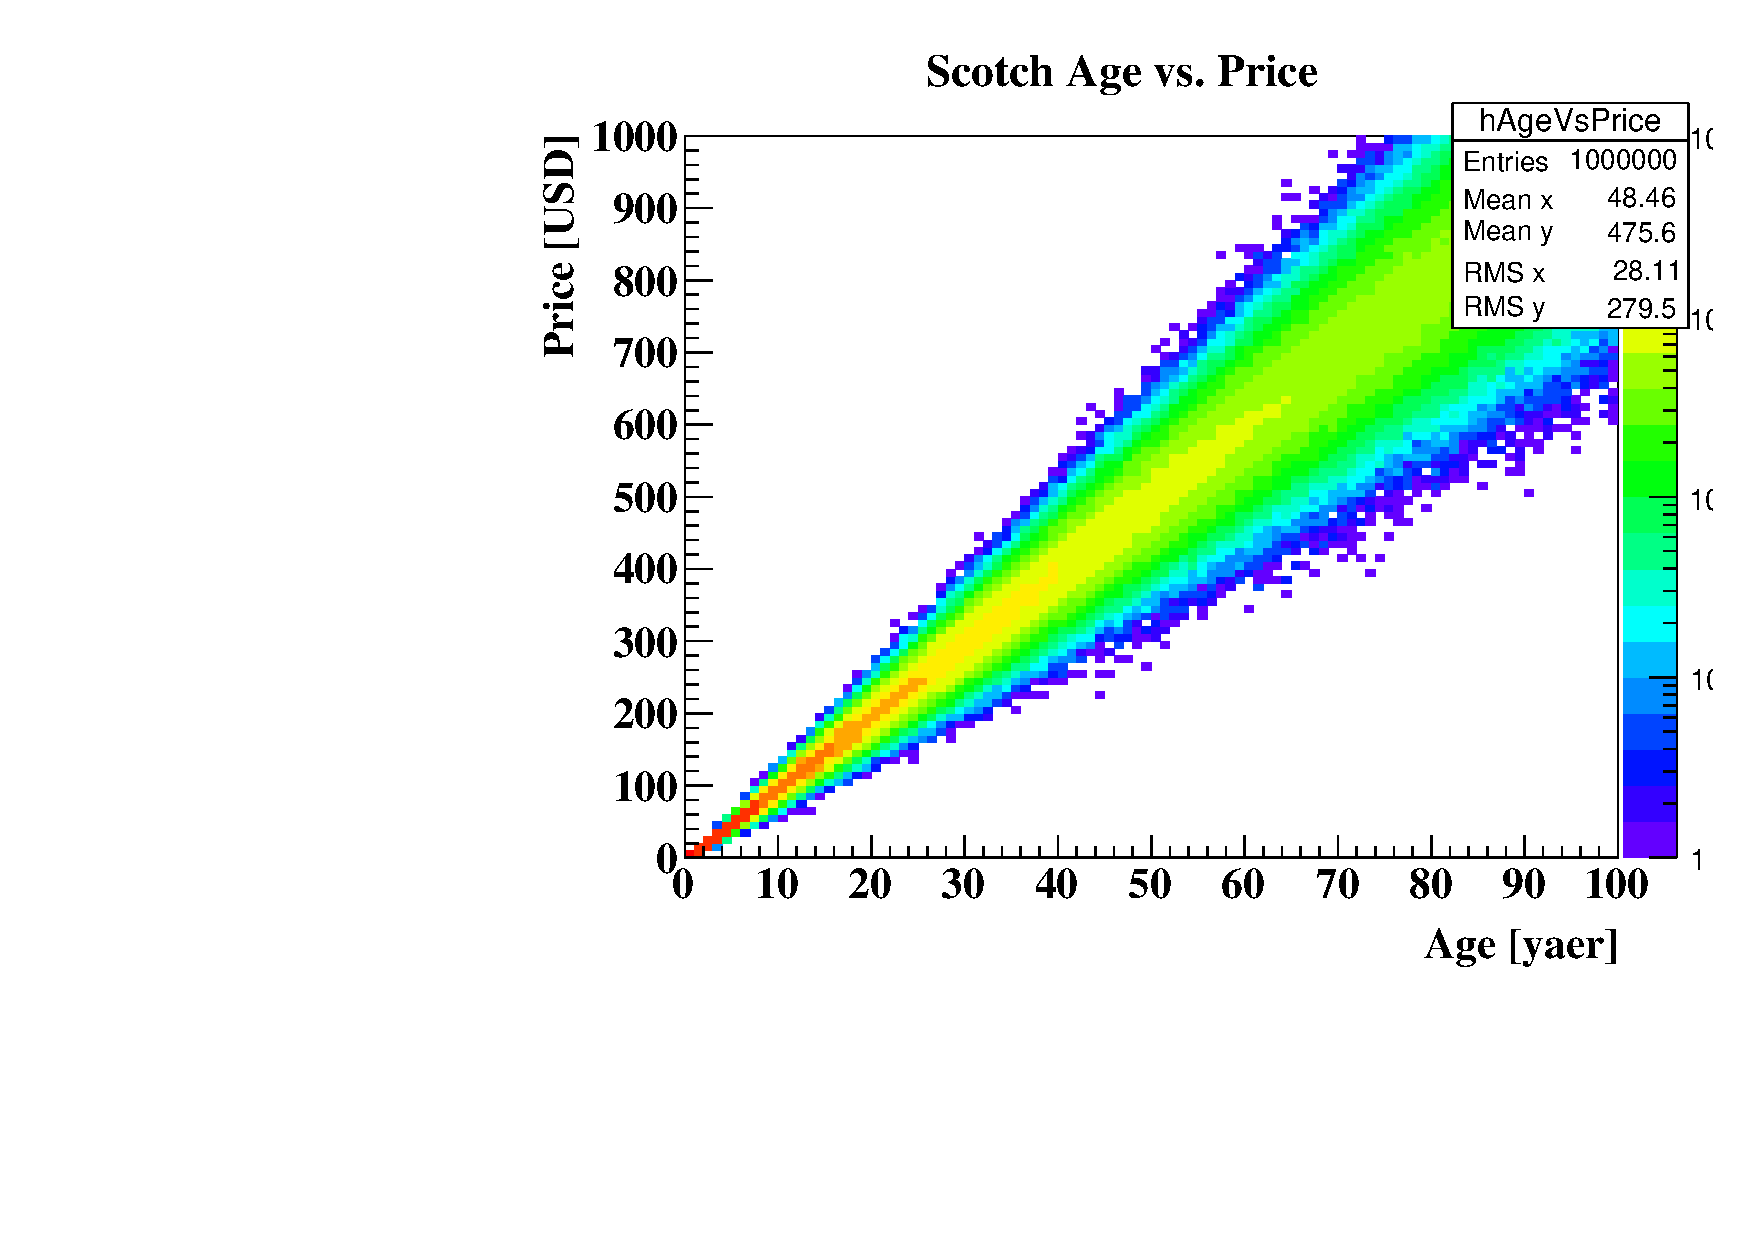
\includegraphics[width=12cm]{./img/ScotchAgeVsPrice.pdf}
\caption{ 
Drawing the age vs. price distribution of {\ttfamily example::Scotch} class from {\ttfamily TTree::Draw}.
}
\end{center}\end{figure}

An example script {\ttfamily mac/example.py} demonstrates how you can:
\begin{itemize}
\item Instantiate {\ttfamily example::Scotch} and save it in a \ROOT file
\item Create a {\ttfamily TTree} of {\ttfamily example::Scotch} for 1e6 entries and save
\item Read-in stored {\ttfamily TTree} and make a very simple access to the stored data product
\item Read-in stored {\ttfamily TTree} and call {\ttfamily TTree::Draw} on the stored data product
\end{itemize}

Note that storing multiple variables into a separate branch of {\ttfamily TTree} (i.e. Ntuple approach)
is much more tedious than storing a class instance as demonstrated in {\ttfamily Scotch::ShipScotch}
function. There, you can find a single line to create a {\ttfamily TTree} branch:
\begin{lstlisting}
tree.Branch("scotch",&data);
\end{lstlisting}
where ``data'' is a {\ttfamily example::Scotch} instance.
With this single line call, all variables in {\ttfamily example::Scotch} instance is stored
with a proper type, and will be readout correctly.

Another myth often people have is that it is very hard to access this object information from
{\ttfamily TTree}. As you can see in the {\ttfamily example.py}, this is completely irrelevant:
you can access the object directly via branch name. A single line in {\ttfamily Python} from
the script is shown below:
\begin{lstlisting}
ch.scotch.Speak()
\end{lstlisting}
which accesses the stored object and calling the class member function {\ttfamily example::Beer::Speak()}.

\subsection{Package Dependency}
The package {\ttfamily Example/Dependent} is prepared to demonstrate how one can make an inter-package 
dependency. In particular, this package depends on {\ttfamily Example/Function} package. Make sure
you have finished building {\ttfamily Example/Function} before building this package.

As you can see in {\ttfamily Stout.h}, the \CPP class {\ttfamily example::Stout} inherits from
{\ttfamily example::Beer}. In order to avoid re-compilation of {\ttfamily example::Beer} class,
we take a usual approach of just {\it linking} the libraries together. Take a look at 
{\ttfamily GNUmakefile}, in particular the following lines:
\begin{lstlisting}
...
INCFLAGS += -I$(LARLITE_USERDEVDIR)/Example
...
LDFLAGS += -L$(LARLITE_LIBDIR) -lExample_Function
\end{lstlisting}
As advertised in the previous section, you must include the path to find {\ttfamily Beer.h} (which
is called from {\ttfamily Stout.h} via {\ttfamily \#include ``Beer.h''}) in {\ttfamily INCFLAGS}, and
both a path and name of a library that contains {\ttfamily example::Beer} class definition in
{\ttfamily LDFLAGS}. 

An example script {\ttfamily mac/example.py} demonstrates an instantiation of {\ttfamily example::Stout}
class and also a call to its base class function {\ttfamily example::Beer::Speak()}.

\subsection{\python in \CPP}
Finally, some users are interested in developing \CPP code to directly operate on \python objects.
An example {\ttfamily Example/PyExample} is prepared to give a tip on how one can write a \CPP
API for \python. This is much better documented as a part of \python documentation:
\begin{center}
{\color{blue}\url{https://docs.python.org/2/c-api/}}
\end{center}

Using a native \python \CPP API is not very easy nor straight forward. Hence in this example,
again, we use \PyROOT binding that makes our life much easier. In short, a difference of two
methods is that you do not have to write your own binding, which is an extra code that has nothing
to do with your algorithm. Finally, that being said, there are other bindings available out there
such as {\ttfamily Cython} (... and \PyROOT uses one of them underneath anyways).

\subsubsection{External Dependnecy}
First of all, you will be using native \python classes, hence you will depend on \python.
Accordingly you have to modify {\ttfamily GNUmakefile}, in particular {\ttfamily INCFLAGS} and
{\ttfamily LDFLAGS}. Notice following 2 lines in {\ttfamily GNUmakefile}:
\begin{lstlisting}
...
INCFLAGS += $(shell python-config --includes)
...
LDFLAGS += $(shell python-config --ldflags)
\end{lstlisting}
each specifying an extra path to find a \python header file and libraries.

\subsubsection{Hiding \python Header From \CINT}
\python header file is called {\ttfamily Python.h}, and is not parse-able via \ROOT \CINT
compiler. So you have to hide it from \CINT dictionary generation step. This can be seen
in {\ttfamily PyExample.h} header file:
\begin{lstlisting}
...
#ifndef __CINT__
// You have to hide native Python header include from CINT                                                                                                                                                  
#include "Python.h"
#endif
...
\end{lstlisting}

You also need to provide two magic lines to forward declare types:
\begin{lstlisting}
...
struct _object;
typedef _object PyObject;
...
\end{lstlisting}
which is for \python generic object pointers to be used (this is a part of \python \CPP API).

\subsubsection{{\ttfamily example::PyExample::Convert}}
The example class {\ttfamily example::PyExample} has an example function to create a
\python list from a \CPP {\ttfamily std::vector<std::string>} object. You can look at the
source code as to how one can do this very simple operation, and take a look at \python
documentation for doing more elaborate operations.

Running {\ttfamily mac/example.py} should show you how this function works.
Obviously you may want to expand the code to work with more advanced \python objects
such as {\ttfamily numpy} array, {\ttfamily matplotlib} axis, and such. The author
does not have much experience to extend too far, but is happy to discuss if you need a help.

\subsection{Documenting Code Using {\ttfamily Doxygen}}
Though this is not everyone's favorite choice, {\ttfamily doxygen} is a popular method to
provide an in-line documentation in the source code. It works pretty nicely with \CPP, and
somewhat at acceptable level with \python. It is the recommended choice for LArSoft to provide
a minimal documentation.

LArLite repositories comes with a doxygen script. You can try generating a documentation
in {\ttfamily Example} directory by typing:
\begin{lstlisting}
  > make doxygen
\end{lstlisting}
({\bf you need doxygen installed in your system!}).

\begin{figure}[htb]\begin{center}
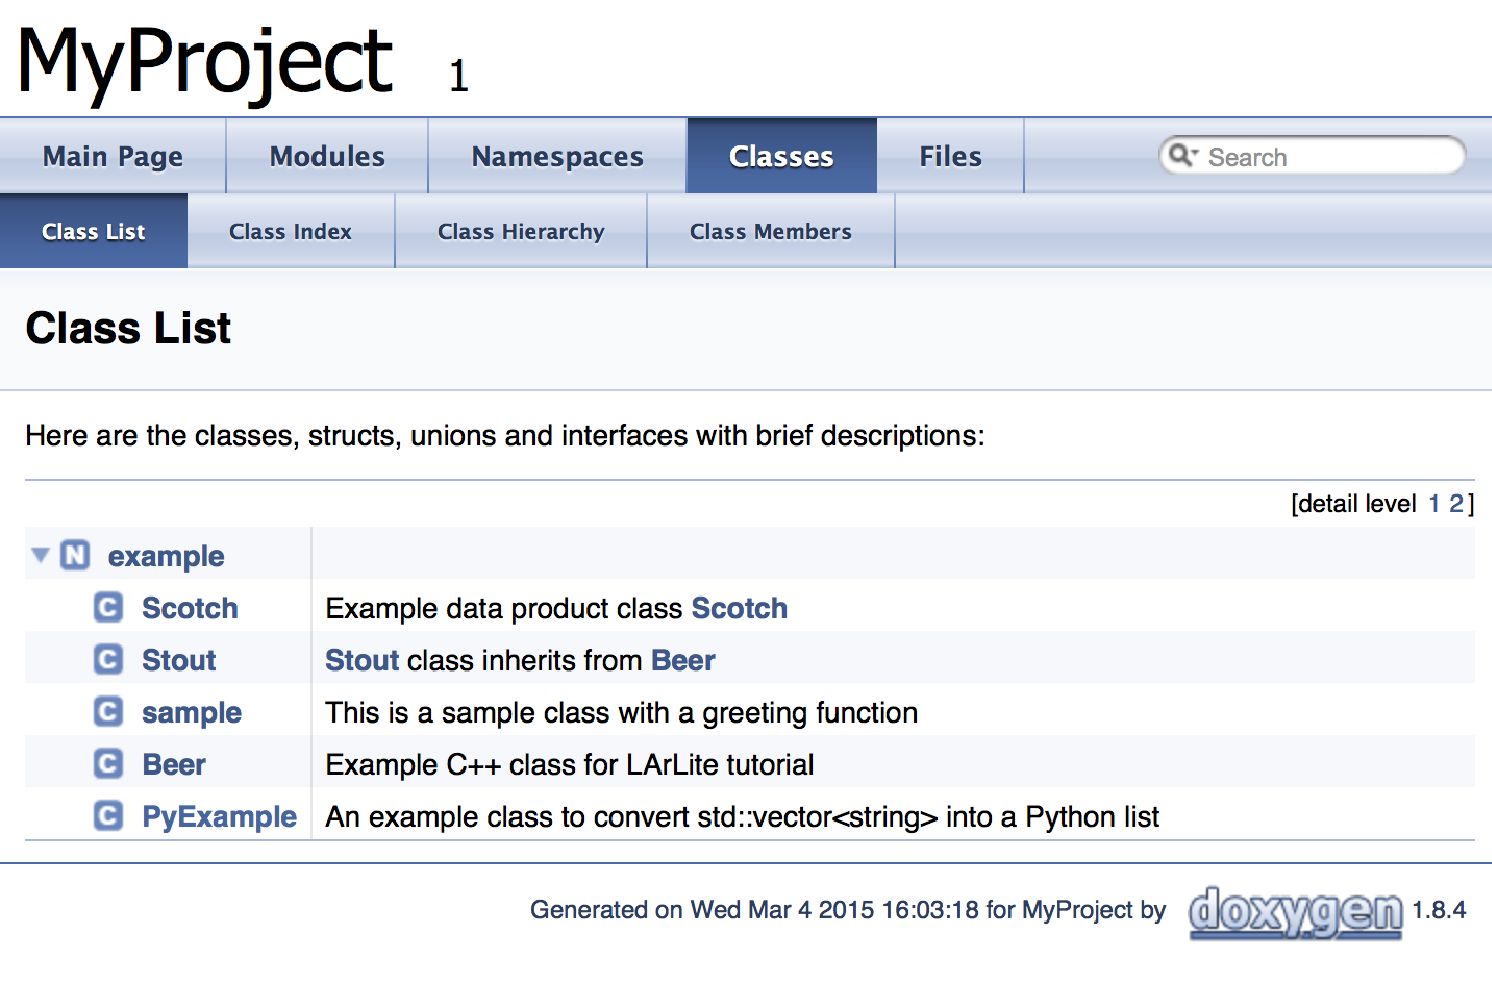
\includegraphics[width=12cm]{./img/doxygen.pdf}
\caption{ 
Doxygen web page generated by ``{\ttfamily make doxygen}'' command for {\ttfamily Example} repository.
}
\end{center}\end{figure}

After successfully running the above command, you should find a chain of HTML files 
to browse through (no internet needed). This way you can also check your doxygen comment
format (whether this is correct or not) before you commit the code. You can look at the
generated documentation using a command like below:
\begin{lstlisting}
  > firefox -a doc/dOxygenMyProject/html/index.html 
\end{lstlisting}
on {\ttfamily Linux} or
\begin{lstlisting}
  > open doc/dOxygenMyProject/html/index.html 
\end{lstlisting}
on {\ttfamily OSX}. The figure shows a generated documentation webpage on the author's laptop.

To understand {\ttfamily doxygen} comment style, refer to their web documentation:
\begin{center}
{\color{blue}\url{http://www.stack.nl/~dimitri/doxygen/manual/docblocks.html}}
\end{center}



% LArUtil package description
\chapter{Core Package: LArUtil}
\label{chap:larutil}

This chapter discuss about how to generating user's own code development space.
In particular following itmes are discussed in the respective order.
\begin{itemize}
\item Getting started: your own code repository
\item A simple \CPP project package 
\item Stuffing your package
\begin{itemize}
  \item Simple \CPP class
  \item \anaunit (see Ch.\ref{chap:analysis}).
  \item \ertool algorithm class (see \ertool documentation)
  \item \ertool filter class (see \ertool documentation)
  \item \ertool analysis class (see \ertool documentation)
  \item \CPP functions
\end{itemize}
\item Details: LArLite build basics
\item Advanced Code Development
\begin{itemize}
  \item \CPP functions outside classes
  \item Inter-package dependence
  \item Data product: storing \CPP class instance in \ROOT file
  \item \python in \CPP (i.e. opposite of \PyROOT)
\end{itemize}
\end{itemize}

\section{Creating Your Repository}
\label{sec:devrepo}

LArLite supports user code development under \UserDev.
More precisely, it is assumed to be under any path that is set to the value of shell environment variable {\ttfamily \$LARLITE\_USERDEVDIR}. 
For the sake of simplicity we stick with \UserDev in this section.

\subsection{Note About \UserDev}
Important note first:
\begin{itemize}
  \item {\ttfamily UserDev/GNUmakefile}, if it exists, is generated by setup.sh and it does not belong to LArLite repository (ignore it).
  \item Some sub-directories belong to LArLite (see below). Some of these depend on LArLite and some don't. It is useful to note them briefly here.
    \begin{itemize}
        \item {\ttfamily BasicTool} contains useful packages like {\ttfamily GeoAlgo} and has no dependency outside
        \item {\ttfamily SelectionTool} contains useful packages like {\ttfamily ERTool} and depends on {\ttfamily BasicTool}
        \item {\ttfamily RecoTool} contains shower reconstruction code and depends on {\ttfamily core}
        \item {\ttfamily LArLiteApp} contains LArLite application from {\ttfamily GeoAlgo} and {\ttfamily ERTool} 
    \end{itemize}
  \item You can create new directories under \UserDev and that won't bother other users. We'll do this below. 
  This is all done through {\ttfamily .gitignore} rule placed under the top directory. 
\end{itemize}

These features of \UserDev are there so that you feel more free to make a mess (sorry, I meant, to develop code) there!

\subsection{Creating Your Sub-Repository in \UserDev}
\label{sec:devrepo:makenew}
Obviously I cannot just say ``do whatever under \UserDev'' and leave: I would love to support a very easy way to develop code (or make a mess) under \UserDev. I will just show you how to do things here:
\begin{lstlisting}
     > llgen_repository MyRepo
\end{lstlisting}
where the execution command is an alias explained in Sec.\ref{sec:configure}.
This should create a new directory called {\ttfamily MyRepo} under \UserDev. 
That is your new repository. As said, this does not affect LArLite repository. 
If you don't want to keep {\ttfamily MyRepo}, simply ``{\ttfamily rm -r}'' it.

Another thing to note here: your repository will contain code and you will compile them, making a compiled shared object library. 
Your repository name will be used to name your library file (if you follow LArLite code generation scripts described in the followings). 
So pick a name that suits for your purpose. You do not want to pick a generic name that might coincide with some other libraries on your machine.

\subsection{What's in MyRepo?}

Your new repository comes with a GNUmakefile (which does nothing for now) and {\ttfamily doc} 
directory with a doxygen script but empty otherwise. Under this space, you can create your ``packages'' as a 
set of \CPP code to be compiled into a library. We will discuss about more later.

\subsection{Creating Your Sub-Repository in {\ttfamily github}}
In the previous section, we created a new repository {\ttfamily MyRepo} under \UserDev. But that's just a directory on your laptop, and you may want to keep it as your code repository using either {\ttfamily svn} or {\ttfamily github} (or anything else you would like to use). Here, I briefly mention how you can do this using {\ttfamily github} because it's very easy given that you already have a {\ttfamily github} account.

First of all, go to {\ttfamily github.com} and create your own repository: go to your {\ttfamily github} account web page, and click on ``+'' symbol that is toward right-top of the web page. Choose ``New repository''. Then enter the repository name you are about to create. Ideally you may want to choose a somewhat unique name as described in Sec.\ref{sec:devrepo:makenew}. You can always remove your repository if you don't like it.

Then checkout your empty repository. As an example, I use my empty repo called {\ttfamily EmptyRepo}.
\begin{lstlisting}
    > cd $LARLITE_USERDEVDIR
    > git clone git@github.com:drinkingkazu/EmptyRepo EmptyRepo
\end{lstlisting}
Now simply run:
\begin{lstlisting}
    > python bin/gen_new_repository EmptyRepo
    > cd EmptyRepo
    > git add .
    > git commit -m ``new repository''
    > gitpush -u origin master
\end{lstlisting}
and you are done!
From the next time, if you want to install LArLite from scratch, simply checkout your repository under UserDev with the same name.

As said many times, of course, your repository is independent of LArLite repository.





\section{Creating a Package}
\label{sec:package}
Here, I assume we are working under {\ttfamily UserDev/MyRepo}. 
In fact, since it's tedious, I will just refer to {\ttfamily MyRepo}.

\subsection{What is a ``Package''?}
``Package'' is a directory under a repository that is compiled and generates one {\bf shred object library}
(i.e. a file with {\ttfamily .so} extension). This library is loaded at a run-time or linked via compiler as one byte code file.
This gives you a sense of what to include in one package: having too many classes (and especially unrelated classes) in one package
means an extra overhead cost for a run-time loading or linking at compilation. In other words, you probably do not want make one 
library per class, but also not one library for all classes. A package should contain a group of \CPP classes/functions which you
think it makes sense to put together.

\subsection{Making a Simple \CPP Package}

Like advertised many times, LArLite was originally a \CPP project play ground for summer students. 
The author thinks it's very important to have an empty \CPP package generator that comes with build system, 
so that a user can focus on writing the algorithm instead of figuring out how to compile and such.

So here it is: there is a \python script to generate an empty \CPP package:
\begin{lstlisting}
    $LARLITE_BASEDIR/bin/gen_package
\end{lstlisting}
This script takes one input argument which is used to name a ``package'', a directory to be created under {\ttfamily MyRepo}.
This script {\bf needs to be executed somewhere under {\ttfamily MyRepo}} (otherwise you'll see an error message).
One can run this script via alias:
\begin{lstlisting}
    > llgen_package MyProject
\end{lstlisting}
which will create a directory {\ttfamily MyRepo/MyProject} that include minimal set of source codes to compile an empty \CPP class. 
You can have your name choice in place of ``MyProject''. After running the command, try:
\begin{lstlisting}
    > cd MyProject
    > make -j4
\end{lstlisting}
This compiles your code and makes {\ttfamily libMyRepo\_MyProject.so} under {\ttfamily lib} directory.
What you compiled is a \CPP class called ``sample'' defined in {\ttfamily sample.h}. 


\subsection{Using in Interpreter}

So how can you ``use'' this \CPP class? You can write a binary executable code, or try out in \CINT or \PyROOT. Here is an example:
\begin{lstlisting}
    > root
    root[0] sample k;
\end{lstlisting}
Above lines work (i.e. your class instance is created) because \CINT is informed about your class. 

\subsection{``Hello World'' Development}
\label{sec:helloworld}
Let's try a simple modification to your class. Here's an example ``hello world'' program using \CPP class. Open {\ttfamily sample.h} and add a {\ttfamily void} function as shown below:
\begin{lstlisting}
class sample{
public:
  /// Default constructor
  sample(){};
  /// Default destructor
  virtual ~sample(){};
  /// Hello world!
  void HelloWorld() { std::cout << ``Hello World!'' << std::endl; }
};
\end{lstlisting}
Save, close and compile (i.e. type ``make''). Now, try the following in \CINT or \PyROOT:
\begin{lstlisting}
    > root
    root[0] sample k;
    root[1] k.HelloWorld();
    Hello World!
    root[2]
\end{lstlisting}

Whenever you want to start a new project with an empty class, you can come back to this example and create your new \CPP project!





\section{Adding Basic \CPP Classes}
\label{sec:expand_package}

As discussed in the previous section, one should populate a package with a group of \CPP classes.
This section describes how to add various types of \CPP classes to your package.

\subsection{Simple \CPP Class}
Sometimes (rather often) you want to generate a completely generic \CPP class for very good reasons: to develop 
some algorithm that is independent of the framework (= easy portability to outside LArLite).

Here is a script for you:
\begin{lstlisting}
    > cd $LARLITE_USERDEVDIR/MyRepo/MyProject
    > llgen_class_empty MyEmptyClass
\end{lstlisting}
Now you should see {\ttfamily MyEmptyClass.h} and {\ttfamily MyEmptyClass.cxx} created under {\ttfamily MyAna}
package. There also made appropriate modification to {\ttfamily LinkDef.h} so that you can just type:
\begin{lstlisting}
    > make -j2
\end{lstlisting}
to compile your new class. Now develop your awesome algorithm and make it a non-empty class ;)

\subsection{\anaunit Class}
If you wish to generate an empty \anaunit class code (to be implemented by you), simply try:
\begin{lstlisting}
    > cd $LARLITE_USERDEVDIR/MyRepo/MyProject
    > llgen_class_anaunit MyAna
\end{lstlisting}

Executing above commands create {\ttfamily MyAna.cxx} and {\ttfamily MyAna.h} (and an appropriate modification to {\ttfamily LinkDef.h}).
Try:
\begin{lstlisting}
    > make -j4
\end{lstlisting}
You just made your new \anaunit class, {\ttfamily MyAna}, whieh inherits from {\ttfamily ana\_base}! 
Your new \anaunit is accessible from \CINT or \PyROOT like any other classes in LArLite:
\begin{lstlisting}
    > root
    root[0] larlite::MyAna my_ana_instance
\end{lstlisting}
Now go ahead and code up this analysis unit, and run with {\ttfamily ana\_processor}! 

\subsubsection{Run Your Analysis Unit: \PyROOT}
\label{sec:yourrunscript}
There is an example \python run script for \anaunit under {\ttfamily mac} directory, called 
{\ttfamily example\_anaunit.py}. You need a LArLite sample \ROOT file to run this program. 
If you have a sample file, say {\ttfamily trial.root}, you can run the program as follows.
\begin{lstlisting}
    > python mac/example_anaunit.py trial.root
\end{lstlisting}

\subsection{\ertool Classes}
Just as we exercised how to add a new \CPP class to a package, there's analogous python scripts to
generate \ertool reconstruction algorithm, filter, and analysis class:
\begin{lstlisting}
    > cd $LARLITE_USERDEVDIR/MyRepo/MyProject
    > llgen_class_erfilter Trial
    > llgen_class_eralgo Trial
    > llgen_class_erana Trial
\end{lstlisting}
Above three commands generate three \CPP classes: {\ttfamily ERFilterTrial}, {\ttfamily ERAlgoTrial}, and {\ttfamily ERAnaTrial}.
These are implementation of base classes defined in \ertool, hence must be used with {\ttfamily ertool::Manager}.
For details, see \ertool documentation (which is to come...)






\section{Understanding the Build}
\label{sec:build_package}
This section covers the basics of how the LArLite build works, aiming to reduce a black-box content for users and developers.
The following topics are ordered such that a topic of interest to more people gets covered first.

\subsection{{\ttfamily Compiler} and {\ttfamily Linker} for Dummies}
Skip if you already know about them, obviously.

Our \CPP source codes are merely descriptions of what we want our computer to do in human-friendly language 
(disagree on ``human-fiendly''? Welcome to the club).
A {\ttfamily compiler} takes in our source code and generate a machine-friendly description, often called as an {\it object file} or {\it byte code}.
When you compile your package in LArLite, you find files with {\ttfamily .o} extension: these are the object files.

Now having many granular object files is not very helpful.
A {\ttfamily linker} allows us to combine multiple object files and create a {\it shared object library} file.
You find such files with {\ttfamily .so} extension under {\ttfamily \$LARLITE\_LIBDIR} if you compiled any package.
The scope of what objects should be put together is really a developer's choice.
In LArLite, this is done per package.
Another (and more important) advantage of shared object libraries kicks in when you compile another code that depends on it.
Say you have a \CPP class {\ttfamily A} and {\ttfamily B} where {\ttfamily B} depends on {\ttfamily A}. 
Once you have {\ttfamily A} compiled with {\ttfamily .so} file, a separate compilation of {\ttfamily B} does not require
a re-compilation of {\ttfamily A}'s source code. Instead, you can {\it link} the {\ttfamily A}'s library upon compilation
of {\ttfamily B}'s library.

In LArLite, we compile files with {\ttfamily .cxx} extensions with a compiler, and create a shared object library using a linker, which
is nothing special compared to any other softwares' build system.

\subsection{{\ttfamily INCFLAGS} and {\ttfamily LDFLAGS}: LArLite Compiler Flags}
In LArLite package's {\ttfamily GNUmakefile}, you may see variables named as {\ttfamily INCFLAGS} and {\ttfamily LDFLAGS} where
the latter may not appear in some simple code packages (i.e. don't worry about not seeing {\ttfamily LDFLAGS} in your {\ttfamily GNUmakefile}).
These are called {\it compiler flags} and passed onto a compiler and linker respectively.

\subsubsection{INCFLAGS}
{\ttfamily INCFLAGS} is used by a compiler to search for files you specify with {\ttfamily \#include} preprocessor command in your source code.
In other words, if your source code calls {\ttfamily \#include <TH1D.h>}, then the directory path which contains {\ttfamily TH1D.h} has to be
added to {\ttfamily INCFLAGS}. The format of {\ttfamily INCFLAGS} is ``-I\$PATH'' where you should replace ``\$PATH'' with the relevant
directory path.

That being said, by default, LArLite includes a \ROOT's include flags.
\ROOT follows a standard method to provide such flags, and you can try this in your installation as well:
\begin{lstlisting}
  > root-config --cflags
\end{lstlisting}
The output of above command is a part of LArLite's default {\ttfamily INCFLAGS}.

\subsubsection{LDFLAGS}
{\ttfamily LDFLAGS} is used by a linker to find libraries to be linked into your package. If your package depends on any externaly compiled
code, for instance a \ROOT class {\ttfamily TH1D}, you have to specify the library to be linked here. The format is 
{\ttfamily -L\$PATH -l\$LIBNAME} where ``\$PATH'' is the directory path that contains a library named ``lib\$LIBNAME.so''. Note that
you should exclude the prefix ``lib'' when you specify it in {\ttfamily LDFLAGS} as that is the standard of how a linker takes in library names.

The default flags in LArLite includes a \ROOT's library flags.
Again, as it was the case for {\ttfamily INCFLAGS}, you can try:
\begin{lstlisting}
  > root-config --libs
\end{lstlisting}
which include most of standard \ROOT libraries such as IO, histogram, TTree, TMatrix, TVector3, etc.

\subsubsection{Flags for LArLite Packages}
You may write a package that depends on existing LArLite code.
One example is an analysis code that inherits from {\ttfamily lalrite::ana\_base}. 
Then you will have to specify {\ttfamily INCFLAGS} and {\ttfamily LDFLAGS}.

Specifying every single {\ttfamily INCFLAGS} and {\ttfamily LDFLAGS} for LArLite code is definitely annoying.
So we follow the popular standard and the following scripts are prepared:
\begin{itemize}
\item {\ttfamily larlite-config} for LArLite's analysis framework
\item {\ttfamily basictool-config} for code under \UserDev/BasicTool 
\item {\ttfamily seltool-config} for code under \UserDev/SelectionTool
\item {\ttfamily recotool-config} for code under \UserDev/RecoTool
\end{itemize}
These scripts can be run with either {\ttfamily --includes} or {\ttfamily --libs} option, and they
simply prints out relevant string to be added to {\ttfamily INCFLAGS} and {\ttfamily LDFLAGS} respectively.
For instance, you may try:
\begin{lstlisting}
  INCFLAGS += $(shell larlite-config --includes)
\end{lstlisting}
and/or
\begin{lstlisting}
  LDFLAGS += $(shell larlite-config --libs)
\end{lstlisting}
in your {\ttfamily GNUmakefile}.

If you use {\ttfamily gen\_class\_anaunit} or similar script, actually, this modification to a {\ttfamily GNUmakefile} is done
by the same script. Hence you do not need to worry about it.

\subsection{Compiler \& Linker Used by LArLite}
Let me make a brief note on how compiler/linker is picked and what default compiler/linker flags are set for LArLite build.

When possible LArLite attempts to use \clang++. In particular this is searched and set when one runs {\ttfamily setup.sh} script.
The configured compiler name is set to a shell environment variable {\ttfamily \$LARLITE\_CXX}.
Further, compiler/linker specific flags are defined in:
\begin{lstlisting}
  > $LARLITE_BASEDIR/Makefile/Makefile.X
\end{lstlisting}
where {\ttfamily X} may be either ``Darwin'' or ``Linux''. 


\section{Advanced Development}
\label{sec:advanced_package}

In this section we follow a prepared example that can be found in:
\begin{center}
{\color{blue}\url{https://github.com/drinkingkazu/Example}}
\end{center}
You might have already checked out this repository as this was mentioned briefly
in the introductory section (see Sec.\ref{sec:build}). 
If not, can certainly checkout under \UserDev:
\begin{lstlisting}
  > cd $LARLITE_USERDEVDIR
  > git clone https://github.com/drinkingkazu/Example
\end{lstlisting}

This repository contains following packages:
\begin{itemize}
\item {\ttfamily Empty} for the simplest example to introduce a simple \CPP class
\item {\ttfamily Function} for demonstrating a \CPP function to be exported into a dictionary
\item {\ttfamily Dependent} for showing how to make inter-package dependencies
\item {\ttfamily DataProduct} as an example of how to store a class instance into a file
\end{itemize}
where we skip the first item, {\ttfamily Empty}, as that has been covered in the previous section.

\subsection{\CPP Functions}
I would like to avoid a confusion: \CPP class is an extension of data structure. In particular,
you do not have to make \CPP class for inventing one or a few functions. Just like we have done
some practice with \CPP class, it would be useful to have \CPP functions in a dictionary.
The point of this package is to show how one can do this.

Take a look at {\ttfamily MyFunctions.h} and {\ttfamily MyFunctions.cxx} source code: there, I defined
functions:
\begin{lstlisting}
  void hello_world();
  Beer Brew(const int age);
\end{lstlisting}
where {\ttfamily example::Beer} is a \CPP class defined in {\ttfamily Beer.h}: it's very very simple class for
playing around unlike the sophisticated name.

Now a compilation works just as expected, and there is nothing special about these functions.
What you may find useful is a format to declare above functions in {\ttfamily LinkDef.h}:
\begin{lstlisting}
#pragma link C++ function  example::hello_world()+;
#pragma link C++ function  example::Brew(const int)+;
\end{lstlisting}
As you can see, a) you do not specify the return type of the function, and b) you only need to specify
the argument types. 

You can try executing an example script {\ttfamily mac/example.py} which calls those functions. 
Take a look at the script's contents and see if that makes sense (... and ask a question if you have any!).
{\color{red}\bf There is one caveat}, however: currently \ROOT seems to require \CPP class compiled
in the same library to be instantiated {\bf before} \CPP functions to be called. The author will
open a ticket for this to be fixed.

\subsection{\ROOT Data Product Class}
Once you get familiar with all LArLite features, you might want to store \CPP object in a file
as a {\ttfamily data product}. The easiest (and recommended) method is to use a \ROOT file.
A rule of the thumb is that any \CPP class that is generated with a \ROOT {\it dictionary} can
be stored in a \ROOT file. You can find details in the \ROOT manual.

If you use LArLite as your code development environment, \ROOT dictionary file is always
generated and built at compilation stage of your package. 

An example can be found in the package {\ttfamily DataProduct}.
There, a data product class called {\ttfamily example::Scotch} is defined. 

\begin{figure}[htb]\begin{center}
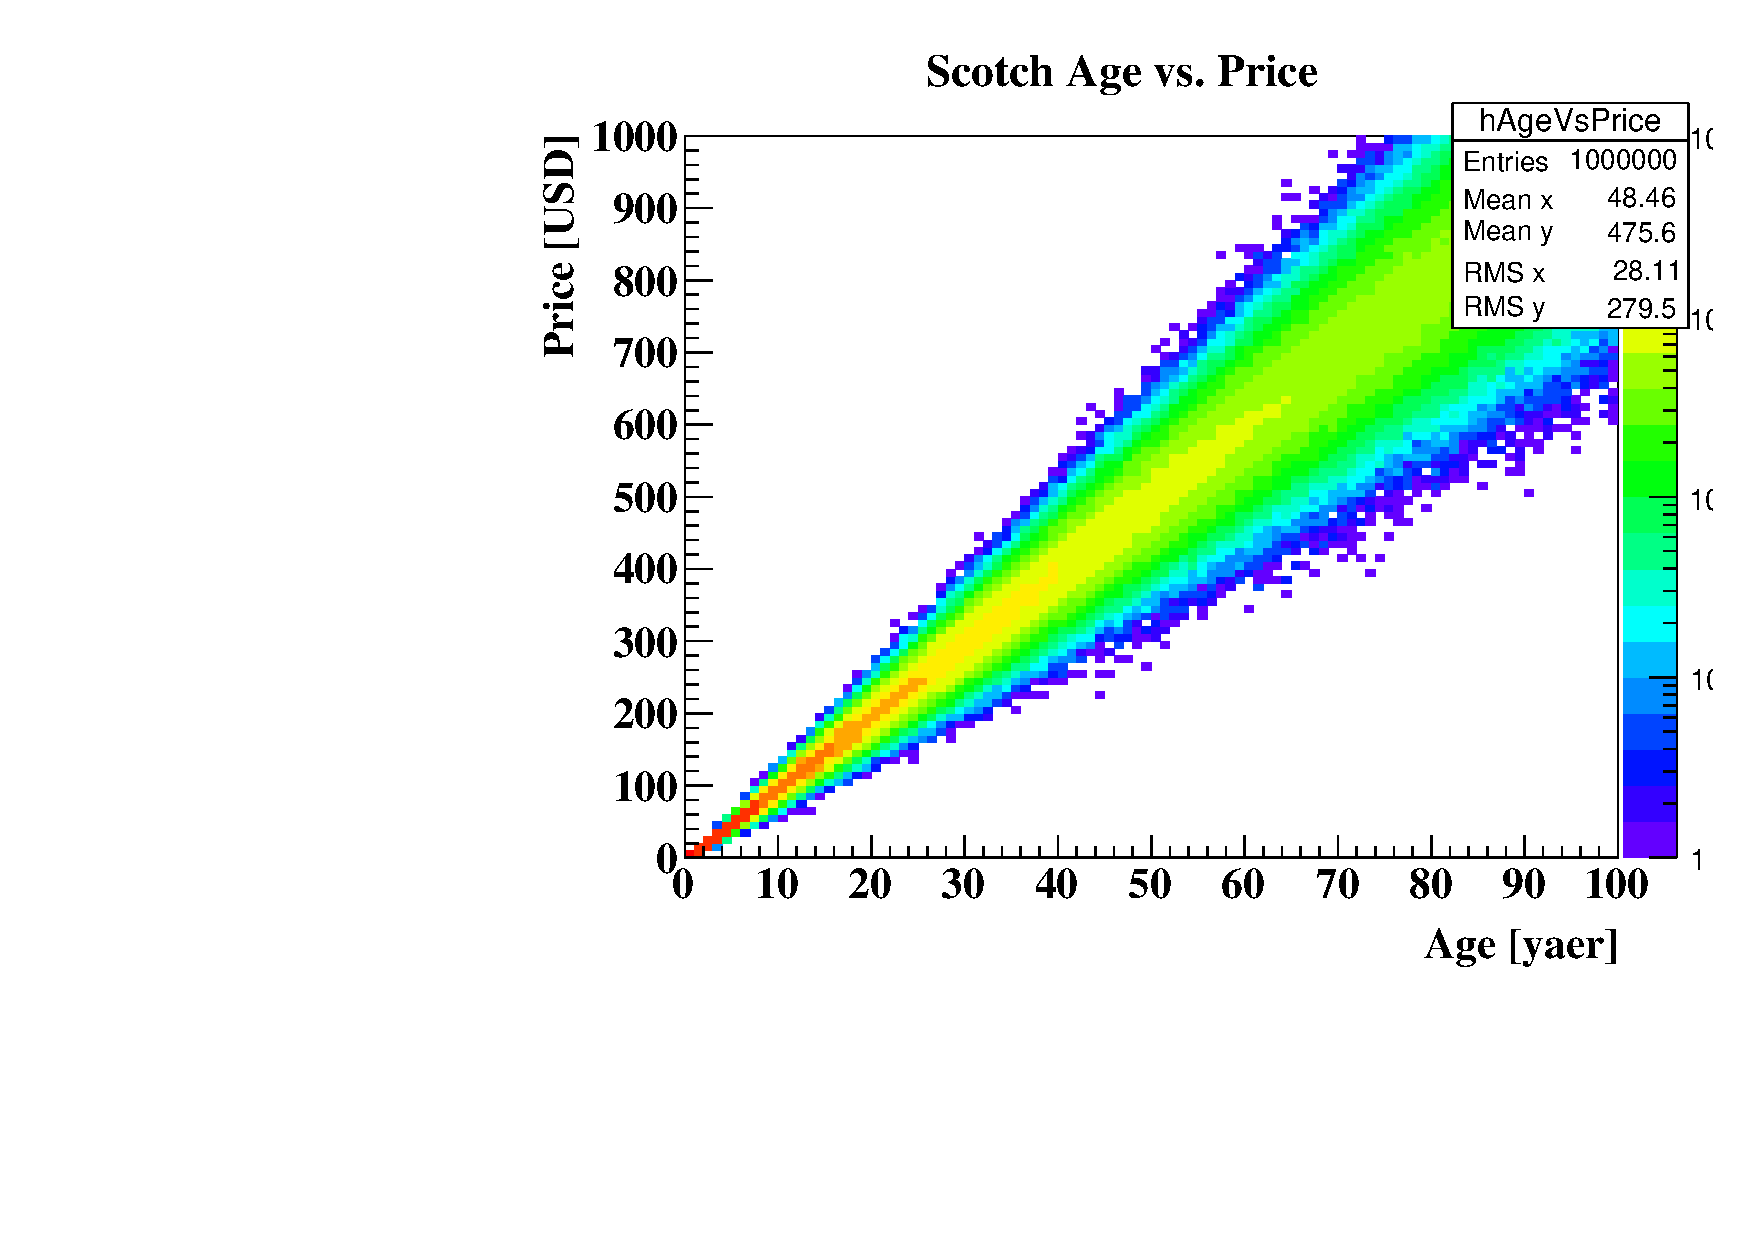
\includegraphics[width=12cm]{./img/ScotchAgeVsPrice.pdf}
\caption{ 
Drawing the age vs. price distribution of {\ttfamily example::Scotch} class from {\ttfamily TTree::Draw}.
}
\end{center}\end{figure}

An example script {\ttfamily mac/example.py} demonstrates how you can:
\begin{itemize}
\item Instantiate {\ttfamily example::Scotch} and save it in a \ROOT file
\item Create a {\ttfamily TTree} of {\ttfamily example::Scotch} for 1e6 entries and save
\item Read-in stored {\ttfamily TTree} and make a very simple access to the stored data product
\item Read-in stored {\ttfamily TTree} and call {\ttfamily TTree::Draw} on the stored data product
\end{itemize}

Note that storing multiple variables into a separate branch of {\ttfamily TTree} (i.e. Ntuple approach)
is much more tedious than storing a class instance as demonstrated in {\ttfamily Scotch::ShipScotch}
function. There, you can find a single line to create a {\ttfamily TTree} branch:
\begin{lstlisting}
tree.Branch("scotch",&data);
\end{lstlisting}
where ``data'' is a {\ttfamily example::Scotch} instance.
With this single line call, all variables in {\ttfamily example::Scotch} instance is stored
with a proper type, and will be readout correctly.

Another myth often people have is that it is very hard to access this object information from
{\ttfamily TTree}. As you can see in the {\ttfamily example.py}, this is completely irrelevant:
you can access the object directly via branch name. A single line in {\ttfamily Python} from
the script is shown below:
\begin{lstlisting}
ch.scotch.Speak()
\end{lstlisting}
which accesses the stored object and calling the class member function {\ttfamily example::Beer::Speak()}.

\subsection{Package Dependency}
The package {\ttfamily Example/Dependent} is prepared to demonstrate how one can make an inter-package 
dependency. In particular, this package depends on {\ttfamily Example/Function} package. Make sure
you have finished building {\ttfamily Example/Function} before building this package.

As you can see in {\ttfamily Stout.h}, the \CPP class {\ttfamily example::Stout} inherits from
{\ttfamily example::Beer}. In order to avoid re-compilation of {\ttfamily example::Beer} class,
we take a usual approach of just {\it linking} the libraries together. Take a look at 
{\ttfamily GNUmakefile}, in particular the following lines:
\begin{lstlisting}
...
INCFLAGS += -I$(LARLITE_USERDEVDIR)/Example
...
LDFLAGS += -L$(LARLITE_LIBDIR) -lExample_Function
\end{lstlisting}
As advertised in the previous section, you must include the path to find {\ttfamily Beer.h} (which
is called from {\ttfamily Stout.h} via {\ttfamily \#include ``Beer.h''}) in {\ttfamily INCFLAGS}, and
both a path and name of a library that contains {\ttfamily example::Beer} class definition in
{\ttfamily LDFLAGS}. 

An example script {\ttfamily mac/example.py} demonstrates an instantiation of {\ttfamily example::Stout}
class and also a call to its base class function {\ttfamily example::Beer::Speak()}.

\subsection{\python in \CPP}
Finally, some users are interested in developing \CPP code to directly operate on \python objects.
An example {\ttfamily Example/PyExample} is prepared to give a tip on how one can write a \CPP
API for \python. This is much better documented as a part of \python documentation:
\begin{center}
{\color{blue}\url{https://docs.python.org/2/c-api/}}
\end{center}

Using a native \python \CPP API is not very easy nor straight forward. Hence in this example,
again, we use \PyROOT binding that makes our life much easier. In short, a difference of two
methods is that you do not have to write your own binding, which is an extra code that has nothing
to do with your algorithm. Finally, that being said, there are other bindings available out there
such as {\ttfamily Cython} (... and \PyROOT uses one of them underneath anyways).

\subsubsection{External Dependnecy}
First of all, you will be using native \python classes, hence you will depend on \python.
Accordingly you have to modify {\ttfamily GNUmakefile}, in particular {\ttfamily INCFLAGS} and
{\ttfamily LDFLAGS}. Notice following 2 lines in {\ttfamily GNUmakefile}:
\begin{lstlisting}
...
INCFLAGS += $(shell python-config --includes)
...
LDFLAGS += $(shell python-config --ldflags)
\end{lstlisting}
each specifying an extra path to find a \python header file and libraries.

\subsubsection{Hiding \python Header From \CINT}
\python header file is called {\ttfamily Python.h}, and is not parse-able via \ROOT \CINT
compiler. So you have to hide it from \CINT dictionary generation step. This can be seen
in {\ttfamily PyExample.h} header file:
\begin{lstlisting}
...
#ifndef __CINT__
// You have to hide native Python header include from CINT                                                                                                                                                  
#include "Python.h"
#endif
...
\end{lstlisting}

You also need to provide two magic lines to forward declare types:
\begin{lstlisting}
...
struct _object;
typedef _object PyObject;
...
\end{lstlisting}
which is for \python generic object pointers to be used (this is a part of \python \CPP API).

\subsubsection{{\ttfamily example::PyExample::Convert}}
The example class {\ttfamily example::PyExample} has an example function to create a
\python list from a \CPP {\ttfamily std::vector<std::string>} object. You can look at the
source code as to how one can do this very simple operation, and take a look at \python
documentation for doing more elaborate operations.

Running {\ttfamily mac/example.py} should show you how this function works.
Obviously you may want to expand the code to work with more advanced \python objects
such as {\ttfamily numpy} array, {\ttfamily matplotlib} axis, and such. The author
does not have much experience to extend too far, but is happy to discuss if you need a help.

\subsection{Documenting Code Using {\ttfamily Doxygen}}
Though this is not everyone's favorite choice, {\ttfamily doxygen} is a popular method to
provide an in-line documentation in the source code. It works pretty nicely with \CPP, and
somewhat at acceptable level with \python. It is the recommended choice for LArSoft to provide
a minimal documentation.

LArLite repositories comes with a doxygen script. You can try generating a documentation
in {\ttfamily Example} directory by typing:
\begin{lstlisting}
  > make doxygen
\end{lstlisting}
({\bf you need doxygen installed in your system!}).

\begin{figure}[htb]\begin{center}
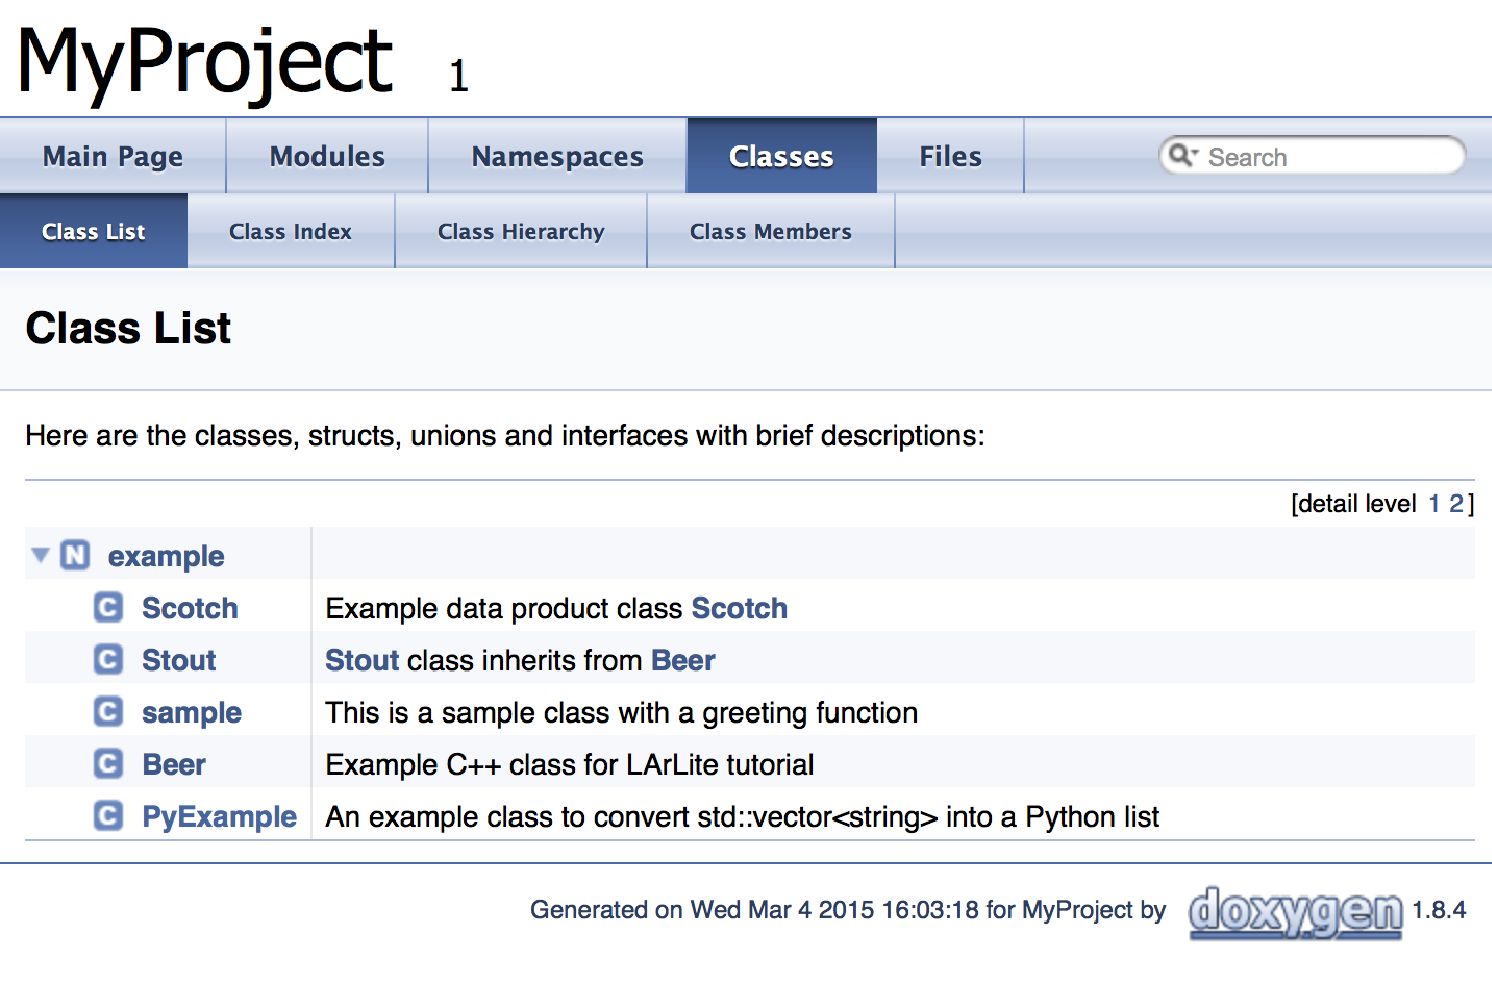
\includegraphics[width=12cm]{./img/doxygen.pdf}
\caption{ 
Doxygen web page generated by ``{\ttfamily make doxygen}'' command for {\ttfamily Example} repository.
}
\end{center}\end{figure}

After successfully running the above command, you should find a chain of HTML files 
to browse through (no internet needed). This way you can also check your doxygen comment
format (whether this is correct or not) before you commit the code. You can look at the
generated documentation using a command like below:
\begin{lstlisting}
  > firefox -a doc/dOxygenMyProject/html/index.html 
\end{lstlisting}
on {\ttfamily Linux} or
\begin{lstlisting}
  > open doc/dOxygenMyProject/html/index.html 
\end{lstlisting}
on {\ttfamily OSX}. The figure shows a generated documentation webpage on the author's laptop.

To understand {\ttfamily doxygen} comment style, refer to their web documentation:
\begin{center}
{\color{blue}\url{http://www.stack.nl/~dimitri/doxygen/manual/docblocks.html}}
\end{center}



% How-to's compilation
\chapter{Generate \& Build Your Package}
\label{chap:generate}

This chapter discuss about how to generating user's own code development space.
In particular following itmes are discussed in the respective order.
\begin{itemize}
\item Getting started: your own code repository
\item A simple \CPP project package 
\item Stuffing your package
\begin{itemize}
  \item Simple \CPP class
  \item \anaunit (see Ch.\ref{chap:analysis}).
  \item \ertool algorithm class (see \ertool documentation)
  \item \ertool filter class (see \ertool documentation)
  \item \ertool analysis class (see \ertool documentation)
  \item \CPP functions
\end{itemize}
\item Details: LArLite build basics
\item Advanced Code Development
\begin{itemize}
  \item \CPP functions outside classes
  \item Inter-package dependence
  \item Data product: storing \CPP class instance in \ROOT file
  \item \python in \CPP (i.e. opposite of \PyROOT)
\end{itemize}
\end{itemize}

\section{Creating Your Repository}
\label{sec:devrepo}

LArLite supports user code development under \UserDev.
More precisely, it is assumed to be under any path that is set to the value of shell environment variable {\ttfamily \$LARLITE\_USERDEVDIR}. 
For the sake of simplicity we stick with \UserDev in this section.

\subsection{Note About \UserDev}
Important note first:
\begin{itemize}
  \item {\ttfamily UserDev/GNUmakefile}, if it exists, is generated by setup.sh and it does not belong to LArLite repository (ignore it).
  \item Some sub-directories belong to LArLite (see below). Some of these depend on LArLite and some don't. It is useful to note them briefly here.
    \begin{itemize}
        \item {\ttfamily BasicTool} contains useful packages like {\ttfamily GeoAlgo} and has no dependency outside
        \item {\ttfamily SelectionTool} contains useful packages like {\ttfamily ERTool} and depends on {\ttfamily BasicTool}
        \item {\ttfamily RecoTool} contains shower reconstruction code and depends on {\ttfamily core}
        \item {\ttfamily LArLiteApp} contains LArLite application from {\ttfamily GeoAlgo} and {\ttfamily ERTool} 
    \end{itemize}
  \item You can create new directories under \UserDev and that won't bother other users. We'll do this below. 
  This is all done through {\ttfamily .gitignore} rule placed under the top directory. 
\end{itemize}

These features of \UserDev are there so that you feel more free to make a mess (sorry, I meant, to develop code) there!

\subsection{Creating Your Sub-Repository in \UserDev}
\label{sec:devrepo:makenew}
Obviously I cannot just say ``do whatever under \UserDev'' and leave: I would love to support a very easy way to develop code (or make a mess) under \UserDev. I will just show you how to do things here:
\begin{lstlisting}
     > llgen_repository MyRepo
\end{lstlisting}
where the execution command is an alias explained in Sec.\ref{sec:configure}.
This should create a new directory called {\ttfamily MyRepo} under \UserDev. 
That is your new repository. As said, this does not affect LArLite repository. 
If you don't want to keep {\ttfamily MyRepo}, simply ``{\ttfamily rm -r}'' it.

Another thing to note here: your repository will contain code and you will compile them, making a compiled shared object library. 
Your repository name will be used to name your library file (if you follow LArLite code generation scripts described in the followings). 
So pick a name that suits for your purpose. You do not want to pick a generic name that might coincide with some other libraries on your machine.

\subsection{What's in MyRepo?}

Your new repository comes with a GNUmakefile (which does nothing for now) and {\ttfamily doc} 
directory with a doxygen script but empty otherwise. Under this space, you can create your ``packages'' as a 
set of \CPP code to be compiled into a library. We will discuss about more later.

\subsection{Creating Your Sub-Repository in {\ttfamily github}}
In the previous section, we created a new repository {\ttfamily MyRepo} under \UserDev. But that's just a directory on your laptop, and you may want to keep it as your code repository using either {\ttfamily svn} or {\ttfamily github} (or anything else you would like to use). Here, I briefly mention how you can do this using {\ttfamily github} because it's very easy given that you already have a {\ttfamily github} account.

First of all, go to {\ttfamily github.com} and create your own repository: go to your {\ttfamily github} account web page, and click on ``+'' symbol that is toward right-top of the web page. Choose ``New repository''. Then enter the repository name you are about to create. Ideally you may want to choose a somewhat unique name as described in Sec.\ref{sec:devrepo:makenew}. You can always remove your repository if you don't like it.

Then checkout your empty repository. As an example, I use my empty repo called {\ttfamily EmptyRepo}.
\begin{lstlisting}
    > cd $LARLITE_USERDEVDIR
    > git clone git@github.com:drinkingkazu/EmptyRepo EmptyRepo
\end{lstlisting}
Now simply run:
\begin{lstlisting}
    > python bin/gen_new_repository EmptyRepo
    > cd EmptyRepo
    > git add .
    > git commit -m ``new repository''
    > gitpush -u origin master
\end{lstlisting}
and you are done!
From the next time, if you want to install LArLite from scratch, simply checkout your repository under UserDev with the same name.

As said many times, of course, your repository is independent of LArLite repository.





\section{Creating a Package}
\label{sec:package}
Here, I assume we are working under {\ttfamily UserDev/MyRepo}. 
In fact, since it's tedious, I will just refer to {\ttfamily MyRepo}.

\subsection{What is a ``Package''?}
``Package'' is a directory under a repository that is compiled and generates one {\bf shred object library}
(i.e. a file with {\ttfamily .so} extension). This library is loaded at a run-time or linked via compiler as one byte code file.
This gives you a sense of what to include in one package: having too many classes (and especially unrelated classes) in one package
means an extra overhead cost for a run-time loading or linking at compilation. In other words, you probably do not want make one 
library per class, but also not one library for all classes. A package should contain a group of \CPP classes/functions which you
think it makes sense to put together.

\subsection{Making a Simple \CPP Package}

Like advertised many times, LArLite was originally a \CPP project play ground for summer students. 
The author thinks it's very important to have an empty \CPP package generator that comes with build system, 
so that a user can focus on writing the algorithm instead of figuring out how to compile and such.

So here it is: there is a \python script to generate an empty \CPP package:
\begin{lstlisting}
    $LARLITE_BASEDIR/bin/gen_package
\end{lstlisting}
This script takes one input argument which is used to name a ``package'', a directory to be created under {\ttfamily MyRepo}.
This script {\bf needs to be executed somewhere under {\ttfamily MyRepo}} (otherwise you'll see an error message).
One can run this script via alias:
\begin{lstlisting}
    > llgen_package MyProject
\end{lstlisting}
which will create a directory {\ttfamily MyRepo/MyProject} that include minimal set of source codes to compile an empty \CPP class. 
You can have your name choice in place of ``MyProject''. After running the command, try:
\begin{lstlisting}
    > cd MyProject
    > make -j4
\end{lstlisting}
This compiles your code and makes {\ttfamily libMyRepo\_MyProject.so} under {\ttfamily lib} directory.
What you compiled is a \CPP class called ``sample'' defined in {\ttfamily sample.h}. 


\subsection{Using in Interpreter}

So how can you ``use'' this \CPP class? You can write a binary executable code, or try out in \CINT or \PyROOT. Here is an example:
\begin{lstlisting}
    > root
    root[0] sample k;
\end{lstlisting}
Above lines work (i.e. your class instance is created) because \CINT is informed about your class. 

\subsection{``Hello World'' Development}
\label{sec:helloworld}
Let's try a simple modification to your class. Here's an example ``hello world'' program using \CPP class. Open {\ttfamily sample.h} and add a {\ttfamily void} function as shown below:
\begin{lstlisting}
class sample{
public:
  /// Default constructor
  sample(){};
  /// Default destructor
  virtual ~sample(){};
  /// Hello world!
  void HelloWorld() { std::cout << ``Hello World!'' << std::endl; }
};
\end{lstlisting}
Save, close and compile (i.e. type ``make''). Now, try the following in \CINT or \PyROOT:
\begin{lstlisting}
    > root
    root[0] sample k;
    root[1] k.HelloWorld();
    Hello World!
    root[2]
\end{lstlisting}

Whenever you want to start a new project with an empty class, you can come back to this example and create your new \CPP project!





\section{Adding Basic \CPP Classes}
\label{sec:expand_package}

As discussed in the previous section, one should populate a package with a group of \CPP classes.
This section describes how to add various types of \CPP classes to your package.

\subsection{Simple \CPP Class}
Sometimes (rather often) you want to generate a completely generic \CPP class for very good reasons: to develop 
some algorithm that is independent of the framework (= easy portability to outside LArLite).

Here is a script for you:
\begin{lstlisting}
    > cd $LARLITE_USERDEVDIR/MyRepo/MyProject
    > llgen_class_empty MyEmptyClass
\end{lstlisting}
Now you should see {\ttfamily MyEmptyClass.h} and {\ttfamily MyEmptyClass.cxx} created under {\ttfamily MyAna}
package. There also made appropriate modification to {\ttfamily LinkDef.h} so that you can just type:
\begin{lstlisting}
    > make -j2
\end{lstlisting}
to compile your new class. Now develop your awesome algorithm and make it a non-empty class ;)

\subsection{\anaunit Class}
If you wish to generate an empty \anaunit class code (to be implemented by you), simply try:
\begin{lstlisting}
    > cd $LARLITE_USERDEVDIR/MyRepo/MyProject
    > llgen_class_anaunit MyAna
\end{lstlisting}

Executing above commands create {\ttfamily MyAna.cxx} and {\ttfamily MyAna.h} (and an appropriate modification to {\ttfamily LinkDef.h}).
Try:
\begin{lstlisting}
    > make -j4
\end{lstlisting}
You just made your new \anaunit class, {\ttfamily MyAna}, whieh inherits from {\ttfamily ana\_base}! 
Your new \anaunit is accessible from \CINT or \PyROOT like any other classes in LArLite:
\begin{lstlisting}
    > root
    root[0] larlite::MyAna my_ana_instance
\end{lstlisting}
Now go ahead and code up this analysis unit, and run with {\ttfamily ana\_processor}! 

\subsubsection{Run Your Analysis Unit: \PyROOT}
\label{sec:yourrunscript}
There is an example \python run script for \anaunit under {\ttfamily mac} directory, called 
{\ttfamily example\_anaunit.py}. You need a LArLite sample \ROOT file to run this program. 
If you have a sample file, say {\ttfamily trial.root}, you can run the program as follows.
\begin{lstlisting}
    > python mac/example_anaunit.py trial.root
\end{lstlisting}

\subsection{\ertool Classes}
Just as we exercised how to add a new \CPP class to a package, there's analogous python scripts to
generate \ertool reconstruction algorithm, filter, and analysis class:
\begin{lstlisting}
    > cd $LARLITE_USERDEVDIR/MyRepo/MyProject
    > llgen_class_erfilter Trial
    > llgen_class_eralgo Trial
    > llgen_class_erana Trial
\end{lstlisting}
Above three commands generate three \CPP classes: {\ttfamily ERFilterTrial}, {\ttfamily ERAlgoTrial}, and {\ttfamily ERAnaTrial}.
These are implementation of base classes defined in \ertool, hence must be used with {\ttfamily ertool::Manager}.
For details, see \ertool documentation (which is to come...)






\section{Understanding the Build}
\label{sec:build_package}
This section covers the basics of how the LArLite build works, aiming to reduce a black-box content for users and developers.
The following topics are ordered such that a topic of interest to more people gets covered first.

\subsection{{\ttfamily Compiler} and {\ttfamily Linker} for Dummies}
Skip if you already know about them, obviously.

Our \CPP source codes are merely descriptions of what we want our computer to do in human-friendly language 
(disagree on ``human-fiendly''? Welcome to the club).
A {\ttfamily compiler} takes in our source code and generate a machine-friendly description, often called as an {\it object file} or {\it byte code}.
When you compile your package in LArLite, you find files with {\ttfamily .o} extension: these are the object files.

Now having many granular object files is not very helpful.
A {\ttfamily linker} allows us to combine multiple object files and create a {\it shared object library} file.
You find such files with {\ttfamily .so} extension under {\ttfamily \$LARLITE\_LIBDIR} if you compiled any package.
The scope of what objects should be put together is really a developer's choice.
In LArLite, this is done per package.
Another (and more important) advantage of shared object libraries kicks in when you compile another code that depends on it.
Say you have a \CPP class {\ttfamily A} and {\ttfamily B} where {\ttfamily B} depends on {\ttfamily A}. 
Once you have {\ttfamily A} compiled with {\ttfamily .so} file, a separate compilation of {\ttfamily B} does not require
a re-compilation of {\ttfamily A}'s source code. Instead, you can {\it link} the {\ttfamily A}'s library upon compilation
of {\ttfamily B}'s library.

In LArLite, we compile files with {\ttfamily .cxx} extensions with a compiler, and create a shared object library using a linker, which
is nothing special compared to any other softwares' build system.

\subsection{{\ttfamily INCFLAGS} and {\ttfamily LDFLAGS}: LArLite Compiler Flags}
In LArLite package's {\ttfamily GNUmakefile}, you may see variables named as {\ttfamily INCFLAGS} and {\ttfamily LDFLAGS} where
the latter may not appear in some simple code packages (i.e. don't worry about not seeing {\ttfamily LDFLAGS} in your {\ttfamily GNUmakefile}).
These are called {\it compiler flags} and passed onto a compiler and linker respectively.

\subsubsection{INCFLAGS}
{\ttfamily INCFLAGS} is used by a compiler to search for files you specify with {\ttfamily \#include} preprocessor command in your source code.
In other words, if your source code calls {\ttfamily \#include <TH1D.h>}, then the directory path which contains {\ttfamily TH1D.h} has to be
added to {\ttfamily INCFLAGS}. The format of {\ttfamily INCFLAGS} is ``-I\$PATH'' where you should replace ``\$PATH'' with the relevant
directory path.

That being said, by default, LArLite includes a \ROOT's include flags.
\ROOT follows a standard method to provide such flags, and you can try this in your installation as well:
\begin{lstlisting}
  > root-config --cflags
\end{lstlisting}
The output of above command is a part of LArLite's default {\ttfamily INCFLAGS}.

\subsubsection{LDFLAGS}
{\ttfamily LDFLAGS} is used by a linker to find libraries to be linked into your package. If your package depends on any externaly compiled
code, for instance a \ROOT class {\ttfamily TH1D}, you have to specify the library to be linked here. The format is 
{\ttfamily -L\$PATH -l\$LIBNAME} where ``\$PATH'' is the directory path that contains a library named ``lib\$LIBNAME.so''. Note that
you should exclude the prefix ``lib'' when you specify it in {\ttfamily LDFLAGS} as that is the standard of how a linker takes in library names.

The default flags in LArLite includes a \ROOT's library flags.
Again, as it was the case for {\ttfamily INCFLAGS}, you can try:
\begin{lstlisting}
  > root-config --libs
\end{lstlisting}
which include most of standard \ROOT libraries such as IO, histogram, TTree, TMatrix, TVector3, etc.

\subsubsection{Flags for LArLite Packages}
You may write a package that depends on existing LArLite code.
One example is an analysis code that inherits from {\ttfamily lalrite::ana\_base}. 
Then you will have to specify {\ttfamily INCFLAGS} and {\ttfamily LDFLAGS}.

Specifying every single {\ttfamily INCFLAGS} and {\ttfamily LDFLAGS} for LArLite code is definitely annoying.
So we follow the popular standard and the following scripts are prepared:
\begin{itemize}
\item {\ttfamily larlite-config} for LArLite's analysis framework
\item {\ttfamily basictool-config} for code under \UserDev/BasicTool 
\item {\ttfamily seltool-config} for code under \UserDev/SelectionTool
\item {\ttfamily recotool-config} for code under \UserDev/RecoTool
\end{itemize}
These scripts can be run with either {\ttfamily --includes} or {\ttfamily --libs} option, and they
simply prints out relevant string to be added to {\ttfamily INCFLAGS} and {\ttfamily LDFLAGS} respectively.
For instance, you may try:
\begin{lstlisting}
  INCFLAGS += $(shell larlite-config --includes)
\end{lstlisting}
and/or
\begin{lstlisting}
  LDFLAGS += $(shell larlite-config --libs)
\end{lstlisting}
in your {\ttfamily GNUmakefile}.

If you use {\ttfamily gen\_class\_anaunit} or similar script, actually, this modification to a {\ttfamily GNUmakefile} is done
by the same script. Hence you do not need to worry about it.

\subsection{Compiler \& Linker Used by LArLite}
Let me make a brief note on how compiler/linker is picked and what default compiler/linker flags are set for LArLite build.

When possible LArLite attempts to use \clang++. In particular this is searched and set when one runs {\ttfamily setup.sh} script.
The configured compiler name is set to a shell environment variable {\ttfamily \$LARLITE\_CXX}.
Further, compiler/linker specific flags are defined in:
\begin{lstlisting}
  > $LARLITE_BASEDIR/Makefile/Makefile.X
\end{lstlisting}
where {\ttfamily X} may be either ``Darwin'' or ``Linux''. 


\section{Advanced Development}
\label{sec:advanced_package}

In this section we follow a prepared example that can be found in:
\begin{center}
{\color{blue}\url{https://github.com/drinkingkazu/Example}}
\end{center}
You might have already checked out this repository as this was mentioned briefly
in the introductory section (see Sec.\ref{sec:build}). 
If not, can certainly checkout under \UserDev:
\begin{lstlisting}
  > cd $LARLITE_USERDEVDIR
  > git clone https://github.com/drinkingkazu/Example
\end{lstlisting}

This repository contains following packages:
\begin{itemize}
\item {\ttfamily Empty} for the simplest example to introduce a simple \CPP class
\item {\ttfamily Function} for demonstrating a \CPP function to be exported into a dictionary
\item {\ttfamily Dependent} for showing how to make inter-package dependencies
\item {\ttfamily DataProduct} as an example of how to store a class instance into a file
\end{itemize}
where we skip the first item, {\ttfamily Empty}, as that has been covered in the previous section.

\subsection{\CPP Functions}
I would like to avoid a confusion: \CPP class is an extension of data structure. In particular,
you do not have to make \CPP class for inventing one or a few functions. Just like we have done
some practice with \CPP class, it would be useful to have \CPP functions in a dictionary.
The point of this package is to show how one can do this.

Take a look at {\ttfamily MyFunctions.h} and {\ttfamily MyFunctions.cxx} source code: there, I defined
functions:
\begin{lstlisting}
  void hello_world();
  Beer Brew(const int age);
\end{lstlisting}
where {\ttfamily example::Beer} is a \CPP class defined in {\ttfamily Beer.h}: it's very very simple class for
playing around unlike the sophisticated name.

Now a compilation works just as expected, and there is nothing special about these functions.
What you may find useful is a format to declare above functions in {\ttfamily LinkDef.h}:
\begin{lstlisting}
#pragma link C++ function  example::hello_world()+;
#pragma link C++ function  example::Brew(const int)+;
\end{lstlisting}
As you can see, a) you do not specify the return type of the function, and b) you only need to specify
the argument types. 

You can try executing an example script {\ttfamily mac/example.py} which calls those functions. 
Take a look at the script's contents and see if that makes sense (... and ask a question if you have any!).
{\color{red}\bf There is one caveat}, however: currently \ROOT seems to require \CPP class compiled
in the same library to be instantiated {\bf before} \CPP functions to be called. The author will
open a ticket for this to be fixed.

\subsection{\ROOT Data Product Class}
Once you get familiar with all LArLite features, you might want to store \CPP object in a file
as a {\ttfamily data product}. The easiest (and recommended) method is to use a \ROOT file.
A rule of the thumb is that any \CPP class that is generated with a \ROOT {\it dictionary} can
be stored in a \ROOT file. You can find details in the \ROOT manual.

If you use LArLite as your code development environment, \ROOT dictionary file is always
generated and built at compilation stage of your package. 

An example can be found in the package {\ttfamily DataProduct}.
There, a data product class called {\ttfamily example::Scotch} is defined. 

\begin{figure}[htb]\begin{center}
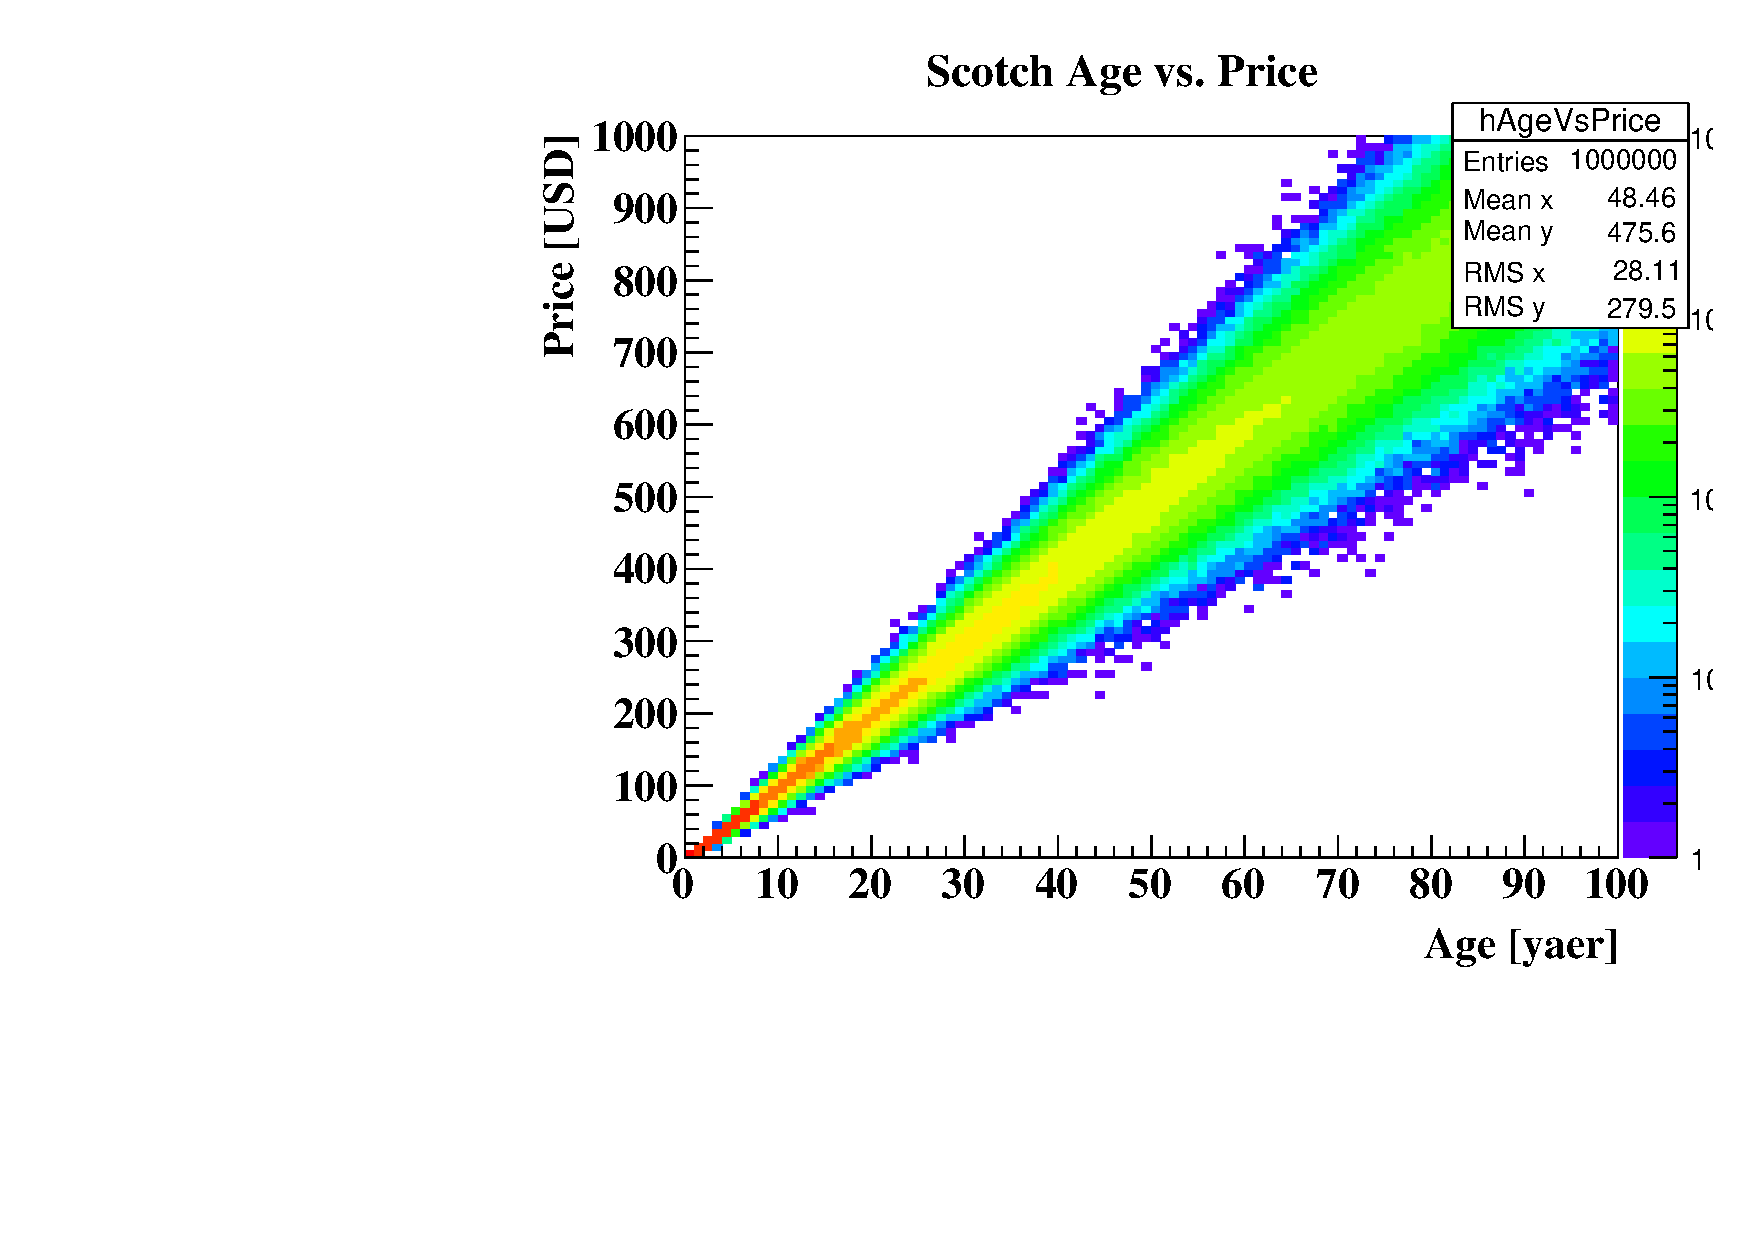
\includegraphics[width=12cm]{./img/ScotchAgeVsPrice.pdf}
\caption{ 
Drawing the age vs. price distribution of {\ttfamily example::Scotch} class from {\ttfamily TTree::Draw}.
}
\end{center}\end{figure}

An example script {\ttfamily mac/example.py} demonstrates how you can:
\begin{itemize}
\item Instantiate {\ttfamily example::Scotch} and save it in a \ROOT file
\item Create a {\ttfamily TTree} of {\ttfamily example::Scotch} for 1e6 entries and save
\item Read-in stored {\ttfamily TTree} and make a very simple access to the stored data product
\item Read-in stored {\ttfamily TTree} and call {\ttfamily TTree::Draw} on the stored data product
\end{itemize}

Note that storing multiple variables into a separate branch of {\ttfamily TTree} (i.e. Ntuple approach)
is much more tedious than storing a class instance as demonstrated in {\ttfamily Scotch::ShipScotch}
function. There, you can find a single line to create a {\ttfamily TTree} branch:
\begin{lstlisting}
tree.Branch("scotch",&data);
\end{lstlisting}
where ``data'' is a {\ttfamily example::Scotch} instance.
With this single line call, all variables in {\ttfamily example::Scotch} instance is stored
with a proper type, and will be readout correctly.

Another myth often people have is that it is very hard to access this object information from
{\ttfamily TTree}. As you can see in the {\ttfamily example.py}, this is completely irrelevant:
you can access the object directly via branch name. A single line in {\ttfamily Python} from
the script is shown below:
\begin{lstlisting}
ch.scotch.Speak()
\end{lstlisting}
which accesses the stored object and calling the class member function {\ttfamily example::Beer::Speak()}.

\subsection{Package Dependency}
The package {\ttfamily Example/Dependent} is prepared to demonstrate how one can make an inter-package 
dependency. In particular, this package depends on {\ttfamily Example/Function} package. Make sure
you have finished building {\ttfamily Example/Function} before building this package.

As you can see in {\ttfamily Stout.h}, the \CPP class {\ttfamily example::Stout} inherits from
{\ttfamily example::Beer}. In order to avoid re-compilation of {\ttfamily example::Beer} class,
we take a usual approach of just {\it linking} the libraries together. Take a look at 
{\ttfamily GNUmakefile}, in particular the following lines:
\begin{lstlisting}
...
INCFLAGS += -I$(LARLITE_USERDEVDIR)/Example
...
LDFLAGS += -L$(LARLITE_LIBDIR) -lExample_Function
\end{lstlisting}
As advertised in the previous section, you must include the path to find {\ttfamily Beer.h} (which
is called from {\ttfamily Stout.h} via {\ttfamily \#include ``Beer.h''}) in {\ttfamily INCFLAGS}, and
both a path and name of a library that contains {\ttfamily example::Beer} class definition in
{\ttfamily LDFLAGS}. 

An example script {\ttfamily mac/example.py} demonstrates an instantiation of {\ttfamily example::Stout}
class and also a call to its base class function {\ttfamily example::Beer::Speak()}.

\subsection{\python in \CPP}
Finally, some users are interested in developing \CPP code to directly operate on \python objects.
An example {\ttfamily Example/PyExample} is prepared to give a tip on how one can write a \CPP
API for \python. This is much better documented as a part of \python documentation:
\begin{center}
{\color{blue}\url{https://docs.python.org/2/c-api/}}
\end{center}

Using a native \python \CPP API is not very easy nor straight forward. Hence in this example,
again, we use \PyROOT binding that makes our life much easier. In short, a difference of two
methods is that you do not have to write your own binding, which is an extra code that has nothing
to do with your algorithm. Finally, that being said, there are other bindings available out there
such as {\ttfamily Cython} (... and \PyROOT uses one of them underneath anyways).

\subsubsection{External Dependnecy}
First of all, you will be using native \python classes, hence you will depend on \python.
Accordingly you have to modify {\ttfamily GNUmakefile}, in particular {\ttfamily INCFLAGS} and
{\ttfamily LDFLAGS}. Notice following 2 lines in {\ttfamily GNUmakefile}:
\begin{lstlisting}
...
INCFLAGS += $(shell python-config --includes)
...
LDFLAGS += $(shell python-config --ldflags)
\end{lstlisting}
each specifying an extra path to find a \python header file and libraries.

\subsubsection{Hiding \python Header From \CINT}
\python header file is called {\ttfamily Python.h}, and is not parse-able via \ROOT \CINT
compiler. So you have to hide it from \CINT dictionary generation step. This can be seen
in {\ttfamily PyExample.h} header file:
\begin{lstlisting}
...
#ifndef __CINT__
// You have to hide native Python header include from CINT                                                                                                                                                  
#include "Python.h"
#endif
...
\end{lstlisting}

You also need to provide two magic lines to forward declare types:
\begin{lstlisting}
...
struct _object;
typedef _object PyObject;
...
\end{lstlisting}
which is for \python generic object pointers to be used (this is a part of \python \CPP API).

\subsubsection{{\ttfamily example::PyExample::Convert}}
The example class {\ttfamily example::PyExample} has an example function to create a
\python list from a \CPP {\ttfamily std::vector<std::string>} object. You can look at the
source code as to how one can do this very simple operation, and take a look at \python
documentation for doing more elaborate operations.

Running {\ttfamily mac/example.py} should show you how this function works.
Obviously you may want to expand the code to work with more advanced \python objects
such as {\ttfamily numpy} array, {\ttfamily matplotlib} axis, and such. The author
does not have much experience to extend too far, but is happy to discuss if you need a help.

\subsection{Documenting Code Using {\ttfamily Doxygen}}
Though this is not everyone's favorite choice, {\ttfamily doxygen} is a popular method to
provide an in-line documentation in the source code. It works pretty nicely with \CPP, and
somewhat at acceptable level with \python. It is the recommended choice for LArSoft to provide
a minimal documentation.

LArLite repositories comes with a doxygen script. You can try generating a documentation
in {\ttfamily Example} directory by typing:
\begin{lstlisting}
  > make doxygen
\end{lstlisting}
({\bf you need doxygen installed in your system!}).

\begin{figure}[htb]\begin{center}
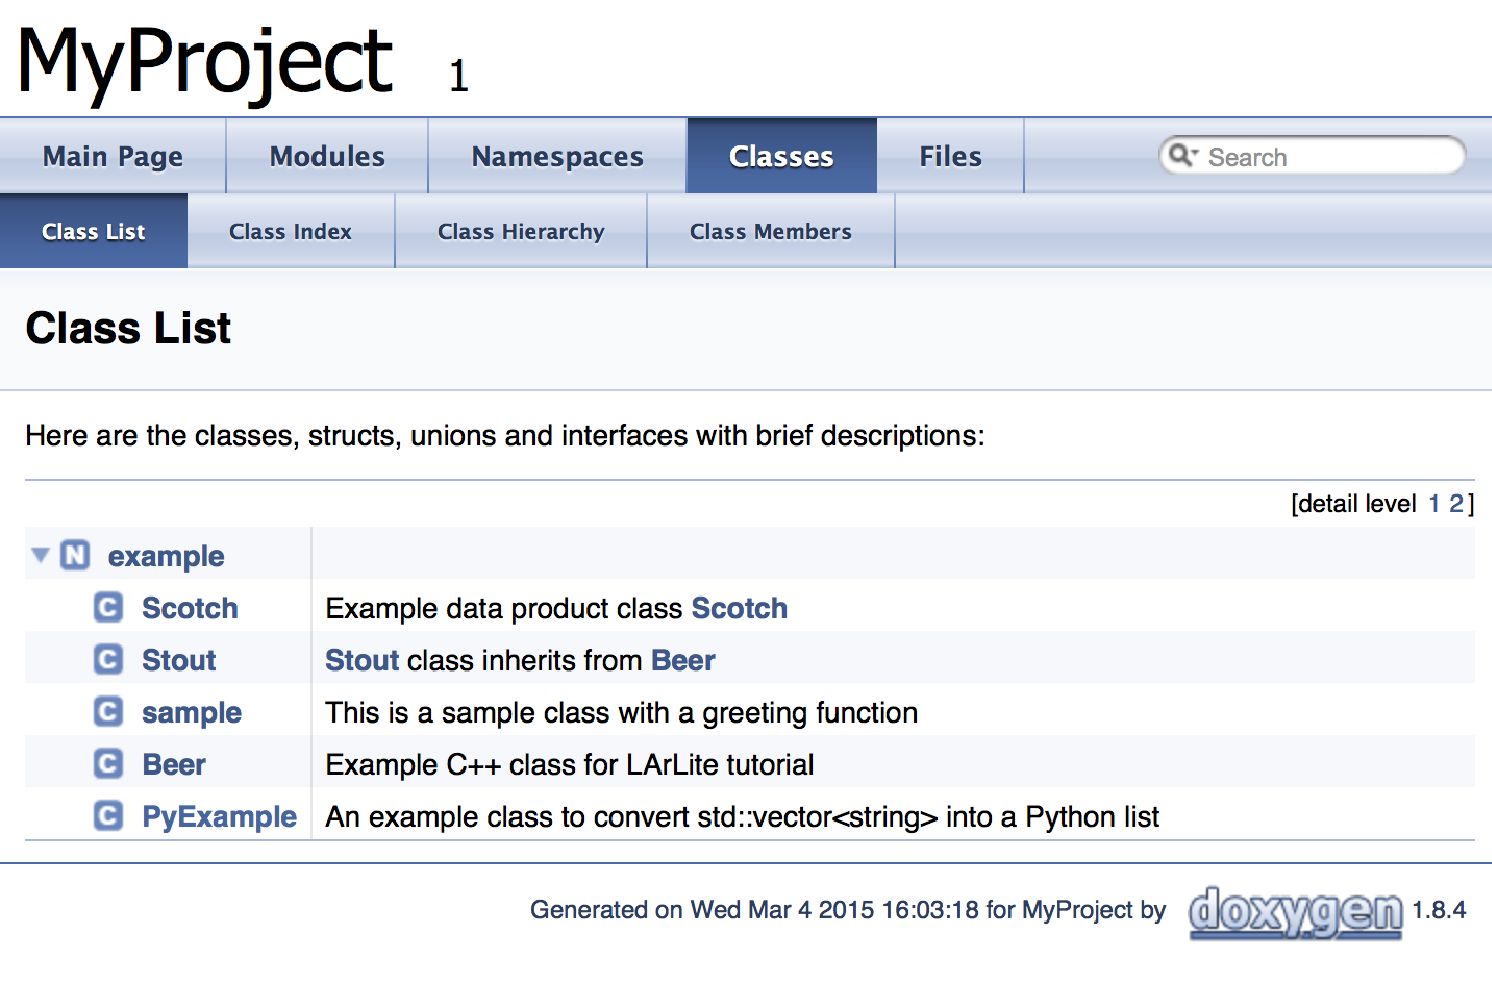
\includegraphics[width=12cm]{./img/doxygen.pdf}
\caption{ 
Doxygen web page generated by ``{\ttfamily make doxygen}'' command for {\ttfamily Example} repository.
}
\end{center}\end{figure}

After successfully running the above command, you should find a chain of HTML files 
to browse through (no internet needed). This way you can also check your doxygen comment
format (whether this is correct or not) before you commit the code. You can look at the
generated documentation using a command like below:
\begin{lstlisting}
  > firefox -a doc/dOxygenMyProject/html/index.html 
\end{lstlisting}
on {\ttfamily Linux} or
\begin{lstlisting}
  > open doc/dOxygenMyProject/html/index.html 
\end{lstlisting}
on {\ttfamily OSX}. The figure shows a generated documentation webpage on the author's laptop.

To understand {\ttfamily doxygen} comment style, refer to their web documentation:
\begin{center}
{\color{blue}\url{http://www.stack.nl/~dimitri/doxygen/manual/docblocks.html}}
\end{center}



% python and LArLight
\chapter{Using LArLight in \python}
\label{chap:pyroot}

This chapter discuss about how to generating user's own code development space.
In particular following itmes are discussed in the respective order.
\begin{itemize}
\item Getting started: your own code repository
\item A simple \CPP project package 
\item Stuffing your package
\begin{itemize}
  \item Simple \CPP class
  \item \anaunit (see Ch.\ref{chap:analysis}).
  \item \ertool algorithm class (see \ertool documentation)
  \item \ertool filter class (see \ertool documentation)
  \item \ertool analysis class (see \ertool documentation)
  \item \CPP functions
\end{itemize}
\item Details: LArLite build basics
\item Advanced Code Development
\begin{itemize}
  \item \CPP functions outside classes
  \item Inter-package dependence
  \item Data product: storing \CPP class instance in \ROOT file
  \item \python in \CPP (i.e. opposite of \PyROOT)
\end{itemize}
\end{itemize}

\section{Creating Your Repository}
\label{sec:devrepo}

LArLite supports user code development under \UserDev.
More precisely, it is assumed to be under any path that is set to the value of shell environment variable {\ttfamily \$LARLITE\_USERDEVDIR}. 
For the sake of simplicity we stick with \UserDev in this section.

\subsection{Note About \UserDev}
Important note first:
\begin{itemize}
  \item {\ttfamily UserDev/GNUmakefile}, if it exists, is generated by setup.sh and it does not belong to LArLite repository (ignore it).
  \item Some sub-directories belong to LArLite (see below). Some of these depend on LArLite and some don't. It is useful to note them briefly here.
    \begin{itemize}
        \item {\ttfamily BasicTool} contains useful packages like {\ttfamily GeoAlgo} and has no dependency outside
        \item {\ttfamily SelectionTool} contains useful packages like {\ttfamily ERTool} and depends on {\ttfamily BasicTool}
        \item {\ttfamily RecoTool} contains shower reconstruction code and depends on {\ttfamily core}
        \item {\ttfamily LArLiteApp} contains LArLite application from {\ttfamily GeoAlgo} and {\ttfamily ERTool} 
    \end{itemize}
  \item You can create new directories under \UserDev and that won't bother other users. We'll do this below. 
  This is all done through {\ttfamily .gitignore} rule placed under the top directory. 
\end{itemize}

These features of \UserDev are there so that you feel more free to make a mess (sorry, I meant, to develop code) there!

\subsection{Creating Your Sub-Repository in \UserDev}
\label{sec:devrepo:makenew}
Obviously I cannot just say ``do whatever under \UserDev'' and leave: I would love to support a very easy way to develop code (or make a mess) under \UserDev. I will just show you how to do things here:
\begin{lstlisting}
     > llgen_repository MyRepo
\end{lstlisting}
where the execution command is an alias explained in Sec.\ref{sec:configure}.
This should create a new directory called {\ttfamily MyRepo} under \UserDev. 
That is your new repository. As said, this does not affect LArLite repository. 
If you don't want to keep {\ttfamily MyRepo}, simply ``{\ttfamily rm -r}'' it.

Another thing to note here: your repository will contain code and you will compile them, making a compiled shared object library. 
Your repository name will be used to name your library file (if you follow LArLite code generation scripts described in the followings). 
So pick a name that suits for your purpose. You do not want to pick a generic name that might coincide with some other libraries on your machine.

\subsection{What's in MyRepo?}

Your new repository comes with a GNUmakefile (which does nothing for now) and {\ttfamily doc} 
directory with a doxygen script but empty otherwise. Under this space, you can create your ``packages'' as a 
set of \CPP code to be compiled into a library. We will discuss about more later.

\subsection{Creating Your Sub-Repository in {\ttfamily github}}
In the previous section, we created a new repository {\ttfamily MyRepo} under \UserDev. But that's just a directory on your laptop, and you may want to keep it as your code repository using either {\ttfamily svn} or {\ttfamily github} (or anything else you would like to use). Here, I briefly mention how you can do this using {\ttfamily github} because it's very easy given that you already have a {\ttfamily github} account.

First of all, go to {\ttfamily github.com} and create your own repository: go to your {\ttfamily github} account web page, and click on ``+'' symbol that is toward right-top of the web page. Choose ``New repository''. Then enter the repository name you are about to create. Ideally you may want to choose a somewhat unique name as described in Sec.\ref{sec:devrepo:makenew}. You can always remove your repository if you don't like it.

Then checkout your empty repository. As an example, I use my empty repo called {\ttfamily EmptyRepo}.
\begin{lstlisting}
    > cd $LARLITE_USERDEVDIR
    > git clone git@github.com:drinkingkazu/EmptyRepo EmptyRepo
\end{lstlisting}
Now simply run:
\begin{lstlisting}
    > python bin/gen_new_repository EmptyRepo
    > cd EmptyRepo
    > git add .
    > git commit -m ``new repository''
    > gitpush -u origin master
\end{lstlisting}
and you are done!
From the next time, if you want to install LArLite from scratch, simply checkout your repository under UserDev with the same name.

As said many times, of course, your repository is independent of LArLite repository.





\section{Creating a Package}
\label{sec:package}
Here, I assume we are working under {\ttfamily UserDev/MyRepo}. 
In fact, since it's tedious, I will just refer to {\ttfamily MyRepo}.

\subsection{What is a ``Package''?}
``Package'' is a directory under a repository that is compiled and generates one {\bf shred object library}
(i.e. a file with {\ttfamily .so} extension). This library is loaded at a run-time or linked via compiler as one byte code file.
This gives you a sense of what to include in one package: having too many classes (and especially unrelated classes) in one package
means an extra overhead cost for a run-time loading or linking at compilation. In other words, you probably do not want make one 
library per class, but also not one library for all classes. A package should contain a group of \CPP classes/functions which you
think it makes sense to put together.

\subsection{Making a Simple \CPP Package}

Like advertised many times, LArLite was originally a \CPP project play ground for summer students. 
The author thinks it's very important to have an empty \CPP package generator that comes with build system, 
so that a user can focus on writing the algorithm instead of figuring out how to compile and such.

So here it is: there is a \python script to generate an empty \CPP package:
\begin{lstlisting}
    $LARLITE_BASEDIR/bin/gen_package
\end{lstlisting}
This script takes one input argument which is used to name a ``package'', a directory to be created under {\ttfamily MyRepo}.
This script {\bf needs to be executed somewhere under {\ttfamily MyRepo}} (otherwise you'll see an error message).
One can run this script via alias:
\begin{lstlisting}
    > llgen_package MyProject
\end{lstlisting}
which will create a directory {\ttfamily MyRepo/MyProject} that include minimal set of source codes to compile an empty \CPP class. 
You can have your name choice in place of ``MyProject''. After running the command, try:
\begin{lstlisting}
    > cd MyProject
    > make -j4
\end{lstlisting}
This compiles your code and makes {\ttfamily libMyRepo\_MyProject.so} under {\ttfamily lib} directory.
What you compiled is a \CPP class called ``sample'' defined in {\ttfamily sample.h}. 


\subsection{Using in Interpreter}

So how can you ``use'' this \CPP class? You can write a binary executable code, or try out in \CINT or \PyROOT. Here is an example:
\begin{lstlisting}
    > root
    root[0] sample k;
\end{lstlisting}
Above lines work (i.e. your class instance is created) because \CINT is informed about your class. 

\subsection{``Hello World'' Development}
\label{sec:helloworld}
Let's try a simple modification to your class. Here's an example ``hello world'' program using \CPP class. Open {\ttfamily sample.h} and add a {\ttfamily void} function as shown below:
\begin{lstlisting}
class sample{
public:
  /// Default constructor
  sample(){};
  /// Default destructor
  virtual ~sample(){};
  /// Hello world!
  void HelloWorld() { std::cout << ``Hello World!'' << std::endl; }
};
\end{lstlisting}
Save, close and compile (i.e. type ``make''). Now, try the following in \CINT or \PyROOT:
\begin{lstlisting}
    > root
    root[0] sample k;
    root[1] k.HelloWorld();
    Hello World!
    root[2]
\end{lstlisting}

Whenever you want to start a new project with an empty class, you can come back to this example and create your new \CPP project!





\section{Adding Basic \CPP Classes}
\label{sec:expand_package}

As discussed in the previous section, one should populate a package with a group of \CPP classes.
This section describes how to add various types of \CPP classes to your package.

\subsection{Simple \CPP Class}
Sometimes (rather often) you want to generate a completely generic \CPP class for very good reasons: to develop 
some algorithm that is independent of the framework (= easy portability to outside LArLite).

Here is a script for you:
\begin{lstlisting}
    > cd $LARLITE_USERDEVDIR/MyRepo/MyProject
    > llgen_class_empty MyEmptyClass
\end{lstlisting}
Now you should see {\ttfamily MyEmptyClass.h} and {\ttfamily MyEmptyClass.cxx} created under {\ttfamily MyAna}
package. There also made appropriate modification to {\ttfamily LinkDef.h} so that you can just type:
\begin{lstlisting}
    > make -j2
\end{lstlisting}
to compile your new class. Now develop your awesome algorithm and make it a non-empty class ;)

\subsection{\anaunit Class}
If you wish to generate an empty \anaunit class code (to be implemented by you), simply try:
\begin{lstlisting}
    > cd $LARLITE_USERDEVDIR/MyRepo/MyProject
    > llgen_class_anaunit MyAna
\end{lstlisting}

Executing above commands create {\ttfamily MyAna.cxx} and {\ttfamily MyAna.h} (and an appropriate modification to {\ttfamily LinkDef.h}).
Try:
\begin{lstlisting}
    > make -j4
\end{lstlisting}
You just made your new \anaunit class, {\ttfamily MyAna}, whieh inherits from {\ttfamily ana\_base}! 
Your new \anaunit is accessible from \CINT or \PyROOT like any other classes in LArLite:
\begin{lstlisting}
    > root
    root[0] larlite::MyAna my_ana_instance
\end{lstlisting}
Now go ahead and code up this analysis unit, and run with {\ttfamily ana\_processor}! 

\subsubsection{Run Your Analysis Unit: \PyROOT}
\label{sec:yourrunscript}
There is an example \python run script for \anaunit under {\ttfamily mac} directory, called 
{\ttfamily example\_anaunit.py}. You need a LArLite sample \ROOT file to run this program. 
If you have a sample file, say {\ttfamily trial.root}, you can run the program as follows.
\begin{lstlisting}
    > python mac/example_anaunit.py trial.root
\end{lstlisting}

\subsection{\ertool Classes}
Just as we exercised how to add a new \CPP class to a package, there's analogous python scripts to
generate \ertool reconstruction algorithm, filter, and analysis class:
\begin{lstlisting}
    > cd $LARLITE_USERDEVDIR/MyRepo/MyProject
    > llgen_class_erfilter Trial
    > llgen_class_eralgo Trial
    > llgen_class_erana Trial
\end{lstlisting}
Above three commands generate three \CPP classes: {\ttfamily ERFilterTrial}, {\ttfamily ERAlgoTrial}, and {\ttfamily ERAnaTrial}.
These are implementation of base classes defined in \ertool, hence must be used with {\ttfamily ertool::Manager}.
For details, see \ertool documentation (which is to come...)






\section{Understanding the Build}
\label{sec:build_package}
This section covers the basics of how the LArLite build works, aiming to reduce a black-box content for users and developers.
The following topics are ordered such that a topic of interest to more people gets covered first.

\subsection{{\ttfamily Compiler} and {\ttfamily Linker} for Dummies}
Skip if you already know about them, obviously.

Our \CPP source codes are merely descriptions of what we want our computer to do in human-friendly language 
(disagree on ``human-fiendly''? Welcome to the club).
A {\ttfamily compiler} takes in our source code and generate a machine-friendly description, often called as an {\it object file} or {\it byte code}.
When you compile your package in LArLite, you find files with {\ttfamily .o} extension: these are the object files.

Now having many granular object files is not very helpful.
A {\ttfamily linker} allows us to combine multiple object files and create a {\it shared object library} file.
You find such files with {\ttfamily .so} extension under {\ttfamily \$LARLITE\_LIBDIR} if you compiled any package.
The scope of what objects should be put together is really a developer's choice.
In LArLite, this is done per package.
Another (and more important) advantage of shared object libraries kicks in when you compile another code that depends on it.
Say you have a \CPP class {\ttfamily A} and {\ttfamily B} where {\ttfamily B} depends on {\ttfamily A}. 
Once you have {\ttfamily A} compiled with {\ttfamily .so} file, a separate compilation of {\ttfamily B} does not require
a re-compilation of {\ttfamily A}'s source code. Instead, you can {\it link} the {\ttfamily A}'s library upon compilation
of {\ttfamily B}'s library.

In LArLite, we compile files with {\ttfamily .cxx} extensions with a compiler, and create a shared object library using a linker, which
is nothing special compared to any other softwares' build system.

\subsection{{\ttfamily INCFLAGS} and {\ttfamily LDFLAGS}: LArLite Compiler Flags}
In LArLite package's {\ttfamily GNUmakefile}, you may see variables named as {\ttfamily INCFLAGS} and {\ttfamily LDFLAGS} where
the latter may not appear in some simple code packages (i.e. don't worry about not seeing {\ttfamily LDFLAGS} in your {\ttfamily GNUmakefile}).
These are called {\it compiler flags} and passed onto a compiler and linker respectively.

\subsubsection{INCFLAGS}
{\ttfamily INCFLAGS} is used by a compiler to search for files you specify with {\ttfamily \#include} preprocessor command in your source code.
In other words, if your source code calls {\ttfamily \#include <TH1D.h>}, then the directory path which contains {\ttfamily TH1D.h} has to be
added to {\ttfamily INCFLAGS}. The format of {\ttfamily INCFLAGS} is ``-I\$PATH'' where you should replace ``\$PATH'' with the relevant
directory path.

That being said, by default, LArLite includes a \ROOT's include flags.
\ROOT follows a standard method to provide such flags, and you can try this in your installation as well:
\begin{lstlisting}
  > root-config --cflags
\end{lstlisting}
The output of above command is a part of LArLite's default {\ttfamily INCFLAGS}.

\subsubsection{LDFLAGS}
{\ttfamily LDFLAGS} is used by a linker to find libraries to be linked into your package. If your package depends on any externaly compiled
code, for instance a \ROOT class {\ttfamily TH1D}, you have to specify the library to be linked here. The format is 
{\ttfamily -L\$PATH -l\$LIBNAME} where ``\$PATH'' is the directory path that contains a library named ``lib\$LIBNAME.so''. Note that
you should exclude the prefix ``lib'' when you specify it in {\ttfamily LDFLAGS} as that is the standard of how a linker takes in library names.

The default flags in LArLite includes a \ROOT's library flags.
Again, as it was the case for {\ttfamily INCFLAGS}, you can try:
\begin{lstlisting}
  > root-config --libs
\end{lstlisting}
which include most of standard \ROOT libraries such as IO, histogram, TTree, TMatrix, TVector3, etc.

\subsubsection{Flags for LArLite Packages}
You may write a package that depends on existing LArLite code.
One example is an analysis code that inherits from {\ttfamily lalrite::ana\_base}. 
Then you will have to specify {\ttfamily INCFLAGS} and {\ttfamily LDFLAGS}.

Specifying every single {\ttfamily INCFLAGS} and {\ttfamily LDFLAGS} for LArLite code is definitely annoying.
So we follow the popular standard and the following scripts are prepared:
\begin{itemize}
\item {\ttfamily larlite-config} for LArLite's analysis framework
\item {\ttfamily basictool-config} for code under \UserDev/BasicTool 
\item {\ttfamily seltool-config} for code under \UserDev/SelectionTool
\item {\ttfamily recotool-config} for code under \UserDev/RecoTool
\end{itemize}
These scripts can be run with either {\ttfamily --includes} or {\ttfamily --libs} option, and they
simply prints out relevant string to be added to {\ttfamily INCFLAGS} and {\ttfamily LDFLAGS} respectively.
For instance, you may try:
\begin{lstlisting}
  INCFLAGS += $(shell larlite-config --includes)
\end{lstlisting}
and/or
\begin{lstlisting}
  LDFLAGS += $(shell larlite-config --libs)
\end{lstlisting}
in your {\ttfamily GNUmakefile}.

If you use {\ttfamily gen\_class\_anaunit} or similar script, actually, this modification to a {\ttfamily GNUmakefile} is done
by the same script. Hence you do not need to worry about it.

\subsection{Compiler \& Linker Used by LArLite}
Let me make a brief note on how compiler/linker is picked and what default compiler/linker flags are set for LArLite build.

When possible LArLite attempts to use \clang++. In particular this is searched and set when one runs {\ttfamily setup.sh} script.
The configured compiler name is set to a shell environment variable {\ttfamily \$LARLITE\_CXX}.
Further, compiler/linker specific flags are defined in:
\begin{lstlisting}
  > $LARLITE_BASEDIR/Makefile/Makefile.X
\end{lstlisting}
where {\ttfamily X} may be either ``Darwin'' or ``Linux''. 


\section{Advanced Development}
\label{sec:advanced_package}

In this section we follow a prepared example that can be found in:
\begin{center}
{\color{blue}\url{https://github.com/drinkingkazu/Example}}
\end{center}
You might have already checked out this repository as this was mentioned briefly
in the introductory section (see Sec.\ref{sec:build}). 
If not, can certainly checkout under \UserDev:
\begin{lstlisting}
  > cd $LARLITE_USERDEVDIR
  > git clone https://github.com/drinkingkazu/Example
\end{lstlisting}

This repository contains following packages:
\begin{itemize}
\item {\ttfamily Empty} for the simplest example to introduce a simple \CPP class
\item {\ttfamily Function} for demonstrating a \CPP function to be exported into a dictionary
\item {\ttfamily Dependent} for showing how to make inter-package dependencies
\item {\ttfamily DataProduct} as an example of how to store a class instance into a file
\end{itemize}
where we skip the first item, {\ttfamily Empty}, as that has been covered in the previous section.

\subsection{\CPP Functions}
I would like to avoid a confusion: \CPP class is an extension of data structure. In particular,
you do not have to make \CPP class for inventing one or a few functions. Just like we have done
some practice with \CPP class, it would be useful to have \CPP functions in a dictionary.
The point of this package is to show how one can do this.

Take a look at {\ttfamily MyFunctions.h} and {\ttfamily MyFunctions.cxx} source code: there, I defined
functions:
\begin{lstlisting}
  void hello_world();
  Beer Brew(const int age);
\end{lstlisting}
where {\ttfamily example::Beer} is a \CPP class defined in {\ttfamily Beer.h}: it's very very simple class for
playing around unlike the sophisticated name.

Now a compilation works just as expected, and there is nothing special about these functions.
What you may find useful is a format to declare above functions in {\ttfamily LinkDef.h}:
\begin{lstlisting}
#pragma link C++ function  example::hello_world()+;
#pragma link C++ function  example::Brew(const int)+;
\end{lstlisting}
As you can see, a) you do not specify the return type of the function, and b) you only need to specify
the argument types. 

You can try executing an example script {\ttfamily mac/example.py} which calls those functions. 
Take a look at the script's contents and see if that makes sense (... and ask a question if you have any!).
{\color{red}\bf There is one caveat}, however: currently \ROOT seems to require \CPP class compiled
in the same library to be instantiated {\bf before} \CPP functions to be called. The author will
open a ticket for this to be fixed.

\subsection{\ROOT Data Product Class}
Once you get familiar with all LArLite features, you might want to store \CPP object in a file
as a {\ttfamily data product}. The easiest (and recommended) method is to use a \ROOT file.
A rule of the thumb is that any \CPP class that is generated with a \ROOT {\it dictionary} can
be stored in a \ROOT file. You can find details in the \ROOT manual.

If you use LArLite as your code development environment, \ROOT dictionary file is always
generated and built at compilation stage of your package. 

An example can be found in the package {\ttfamily DataProduct}.
There, a data product class called {\ttfamily example::Scotch} is defined. 

\begin{figure}[htb]\begin{center}
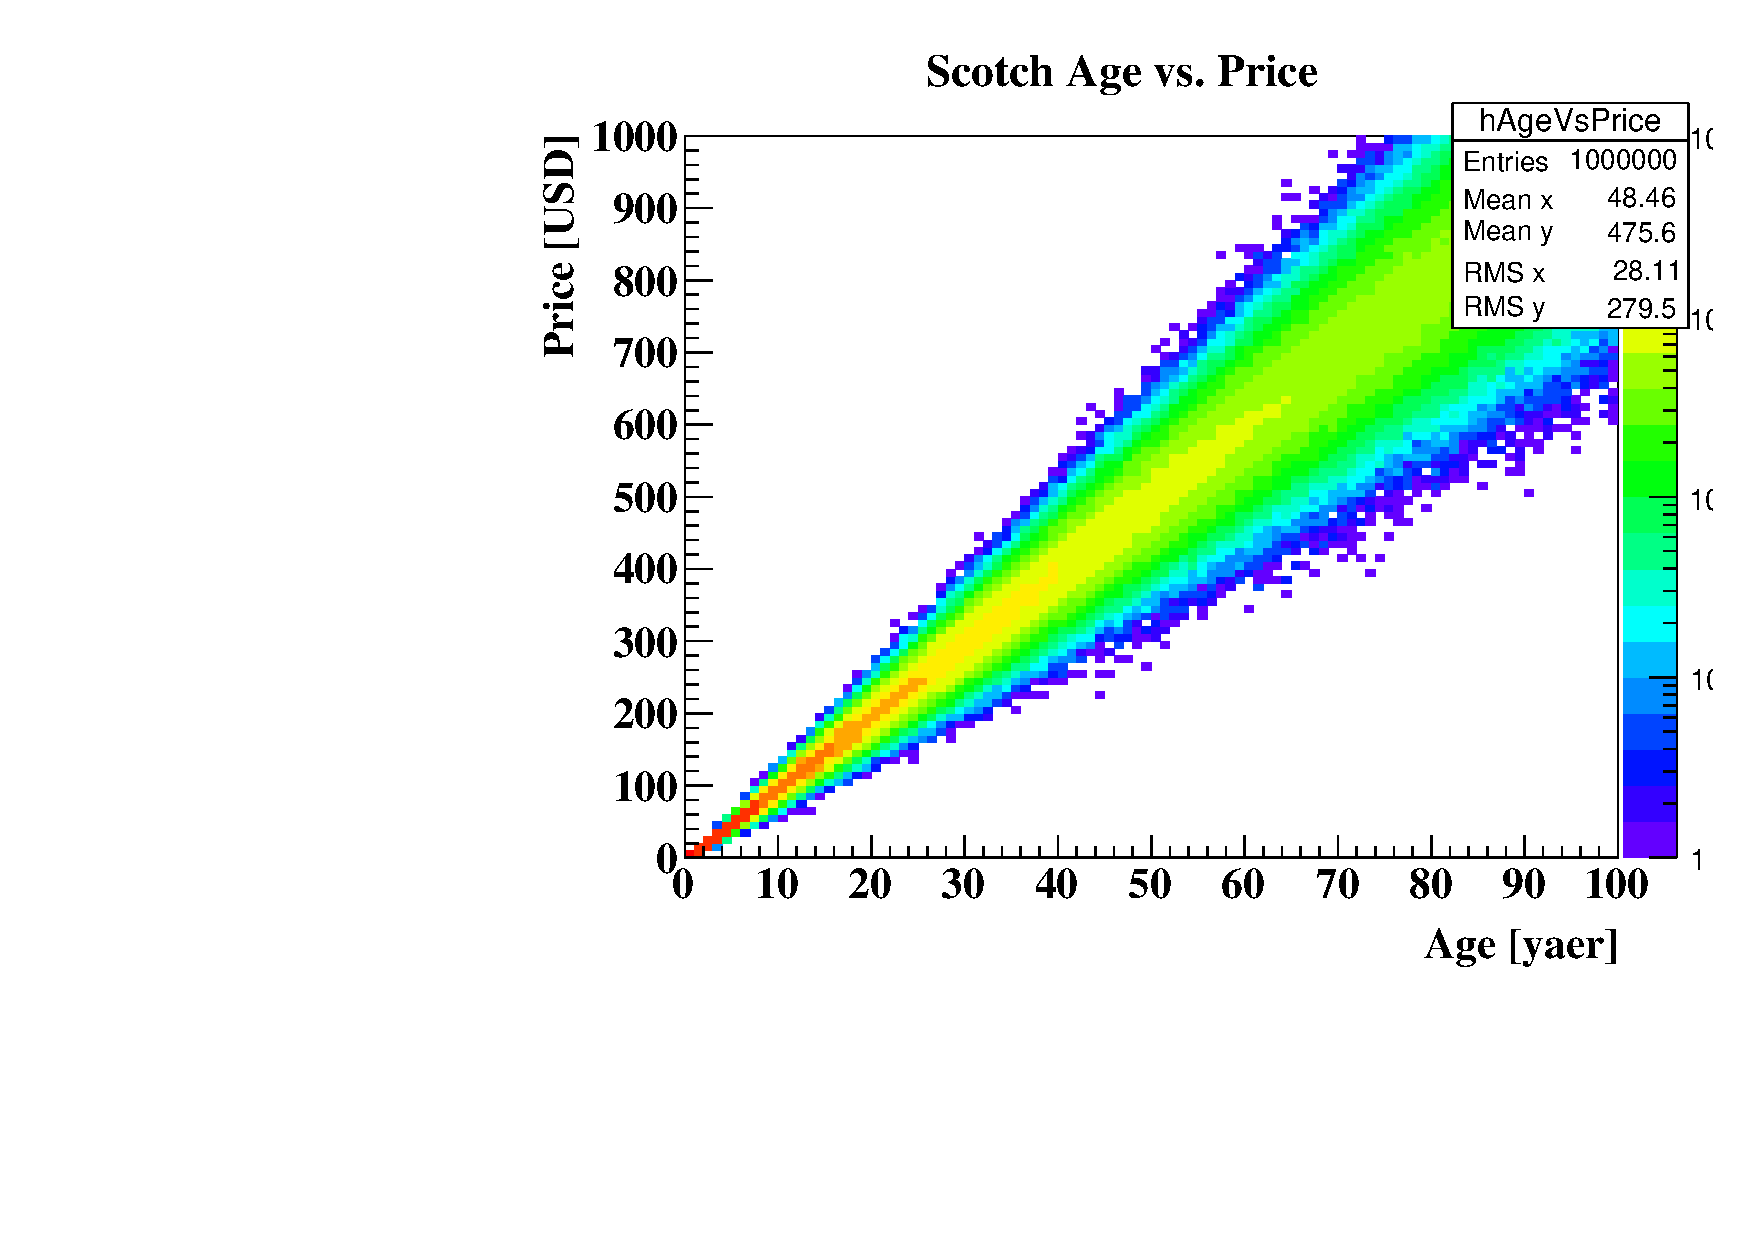
\includegraphics[width=12cm]{./img/ScotchAgeVsPrice.pdf}
\caption{ 
Drawing the age vs. price distribution of {\ttfamily example::Scotch} class from {\ttfamily TTree::Draw}.
}
\end{center}\end{figure}

An example script {\ttfamily mac/example.py} demonstrates how you can:
\begin{itemize}
\item Instantiate {\ttfamily example::Scotch} and save it in a \ROOT file
\item Create a {\ttfamily TTree} of {\ttfamily example::Scotch} for 1e6 entries and save
\item Read-in stored {\ttfamily TTree} and make a very simple access to the stored data product
\item Read-in stored {\ttfamily TTree} and call {\ttfamily TTree::Draw} on the stored data product
\end{itemize}

Note that storing multiple variables into a separate branch of {\ttfamily TTree} (i.e. Ntuple approach)
is much more tedious than storing a class instance as demonstrated in {\ttfamily Scotch::ShipScotch}
function. There, you can find a single line to create a {\ttfamily TTree} branch:
\begin{lstlisting}
tree.Branch("scotch",&data);
\end{lstlisting}
where ``data'' is a {\ttfamily example::Scotch} instance.
With this single line call, all variables in {\ttfamily example::Scotch} instance is stored
with a proper type, and will be readout correctly.

Another myth often people have is that it is very hard to access this object information from
{\ttfamily TTree}. As you can see in the {\ttfamily example.py}, this is completely irrelevant:
you can access the object directly via branch name. A single line in {\ttfamily Python} from
the script is shown below:
\begin{lstlisting}
ch.scotch.Speak()
\end{lstlisting}
which accesses the stored object and calling the class member function {\ttfamily example::Beer::Speak()}.

\subsection{Package Dependency}
The package {\ttfamily Example/Dependent} is prepared to demonstrate how one can make an inter-package 
dependency. In particular, this package depends on {\ttfamily Example/Function} package. Make sure
you have finished building {\ttfamily Example/Function} before building this package.

As you can see in {\ttfamily Stout.h}, the \CPP class {\ttfamily example::Stout} inherits from
{\ttfamily example::Beer}. In order to avoid re-compilation of {\ttfamily example::Beer} class,
we take a usual approach of just {\it linking} the libraries together. Take a look at 
{\ttfamily GNUmakefile}, in particular the following lines:
\begin{lstlisting}
...
INCFLAGS += -I$(LARLITE_USERDEVDIR)/Example
...
LDFLAGS += -L$(LARLITE_LIBDIR) -lExample_Function
\end{lstlisting}
As advertised in the previous section, you must include the path to find {\ttfamily Beer.h} (which
is called from {\ttfamily Stout.h} via {\ttfamily \#include ``Beer.h''}) in {\ttfamily INCFLAGS}, and
both a path and name of a library that contains {\ttfamily example::Beer} class definition in
{\ttfamily LDFLAGS}. 

An example script {\ttfamily mac/example.py} demonstrates an instantiation of {\ttfamily example::Stout}
class and also a call to its base class function {\ttfamily example::Beer::Speak()}.

\subsection{\python in \CPP}
Finally, some users are interested in developing \CPP code to directly operate on \python objects.
An example {\ttfamily Example/PyExample} is prepared to give a tip on how one can write a \CPP
API for \python. This is much better documented as a part of \python documentation:
\begin{center}
{\color{blue}\url{https://docs.python.org/2/c-api/}}
\end{center}

Using a native \python \CPP API is not very easy nor straight forward. Hence in this example,
again, we use \PyROOT binding that makes our life much easier. In short, a difference of two
methods is that you do not have to write your own binding, which is an extra code that has nothing
to do with your algorithm. Finally, that being said, there are other bindings available out there
such as {\ttfamily Cython} (... and \PyROOT uses one of them underneath anyways).

\subsubsection{External Dependnecy}
First of all, you will be using native \python classes, hence you will depend on \python.
Accordingly you have to modify {\ttfamily GNUmakefile}, in particular {\ttfamily INCFLAGS} and
{\ttfamily LDFLAGS}. Notice following 2 lines in {\ttfamily GNUmakefile}:
\begin{lstlisting}
...
INCFLAGS += $(shell python-config --includes)
...
LDFLAGS += $(shell python-config --ldflags)
\end{lstlisting}
each specifying an extra path to find a \python header file and libraries.

\subsubsection{Hiding \python Header From \CINT}
\python header file is called {\ttfamily Python.h}, and is not parse-able via \ROOT \CINT
compiler. So you have to hide it from \CINT dictionary generation step. This can be seen
in {\ttfamily PyExample.h} header file:
\begin{lstlisting}
...
#ifndef __CINT__
// You have to hide native Python header include from CINT                                                                                                                                                  
#include "Python.h"
#endif
...
\end{lstlisting}

You also need to provide two magic lines to forward declare types:
\begin{lstlisting}
...
struct _object;
typedef _object PyObject;
...
\end{lstlisting}
which is for \python generic object pointers to be used (this is a part of \python \CPP API).

\subsubsection{{\ttfamily example::PyExample::Convert}}
The example class {\ttfamily example::PyExample} has an example function to create a
\python list from a \CPP {\ttfamily std::vector<std::string>} object. You can look at the
source code as to how one can do this very simple operation, and take a look at \python
documentation for doing more elaborate operations.

Running {\ttfamily mac/example.py} should show you how this function works.
Obviously you may want to expand the code to work with more advanced \python objects
such as {\ttfamily numpy} array, {\ttfamily matplotlib} axis, and such. The author
does not have much experience to extend too far, but is happy to discuss if you need a help.

\subsection{Documenting Code Using {\ttfamily Doxygen}}
Though this is not everyone's favorite choice, {\ttfamily doxygen} is a popular method to
provide an in-line documentation in the source code. It works pretty nicely with \CPP, and
somewhat at acceptable level with \python. It is the recommended choice for LArSoft to provide
a minimal documentation.

LArLite repositories comes with a doxygen script. You can try generating a documentation
in {\ttfamily Example} directory by typing:
\begin{lstlisting}
  > make doxygen
\end{lstlisting}
({\bf you need doxygen installed in your system!}).

\begin{figure}[htb]\begin{center}
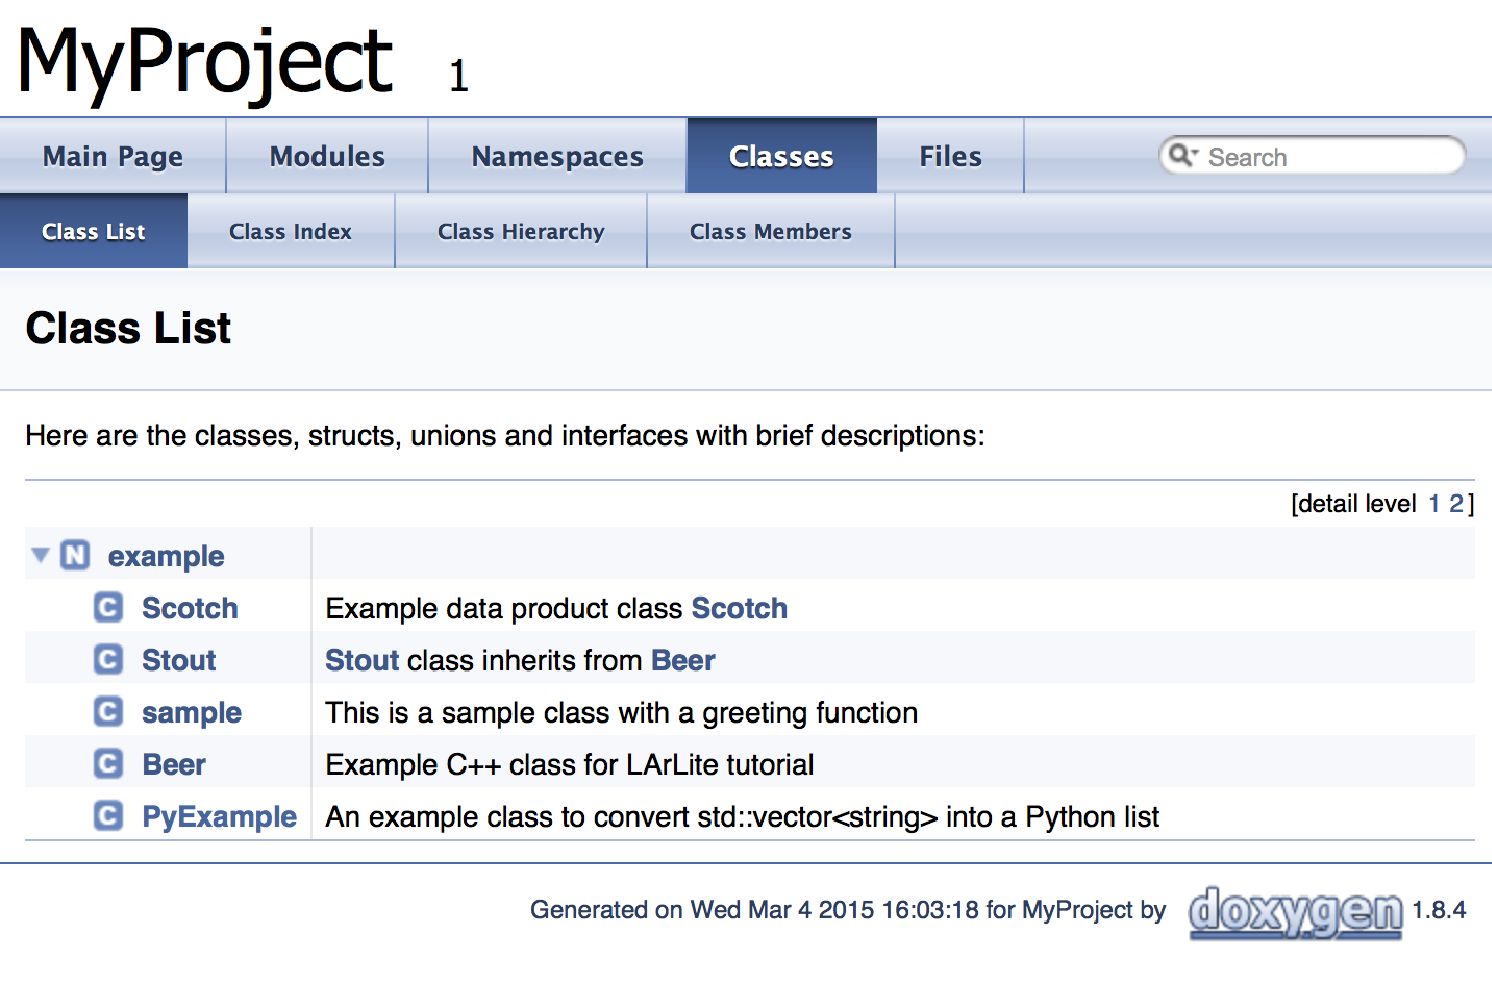
\includegraphics[width=12cm]{./img/doxygen.pdf}
\caption{ 
Doxygen web page generated by ``{\ttfamily make doxygen}'' command for {\ttfamily Example} repository.
}
\end{center}\end{figure}

After successfully running the above command, you should find a chain of HTML files 
to browse through (no internet needed). This way you can also check your doxygen comment
format (whether this is correct or not) before you commit the code. You can look at the
generated documentation using a command like below:
\begin{lstlisting}
  > firefox -a doc/dOxygenMyProject/html/index.html 
\end{lstlisting}
on {\ttfamily Linux} or
\begin{lstlisting}
  > open doc/dOxygenMyProject/html/index.html 
\end{lstlisting}
on {\ttfamily OSX}. The figure shows a generated documentation webpage on the author's laptop.

To understand {\ttfamily doxygen} comment style, refer to their web documentation:
\begin{center}
{\color{blue}\url{http://www.stack.nl/~dimitri/doxygen/manual/docblocks.html}}
\end{center}



% LArSoft => LArLight converter
\chapter{Where is LArLight Data File?}
\label{chap:datafile}

This chapter discuss about how to generating user's own code development space.
In particular following itmes are discussed in the respective order.
\begin{itemize}
\item Getting started: your own code repository
\item A simple \CPP project package 
\item Stuffing your package
\begin{itemize}
  \item Simple \CPP class
  \item \anaunit (see Ch.\ref{chap:analysis}).
  \item \ertool algorithm class (see \ertool documentation)
  \item \ertool filter class (see \ertool documentation)
  \item \ertool analysis class (see \ertool documentation)
  \item \CPP functions
\end{itemize}
\item Details: LArLite build basics
\item Advanced Code Development
\begin{itemize}
  \item \CPP functions outside classes
  \item Inter-package dependence
  \item Data product: storing \CPP class instance in \ROOT file
  \item \python in \CPP (i.e. opposite of \PyROOT)
\end{itemize}
\end{itemize}

\section{Creating Your Repository}
\label{sec:devrepo}

LArLite supports user code development under \UserDev.
More precisely, it is assumed to be under any path that is set to the value of shell environment variable {\ttfamily \$LARLITE\_USERDEVDIR}. 
For the sake of simplicity we stick with \UserDev in this section.

\subsection{Note About \UserDev}
Important note first:
\begin{itemize}
  \item {\ttfamily UserDev/GNUmakefile}, if it exists, is generated by setup.sh and it does not belong to LArLite repository (ignore it).
  \item Some sub-directories belong to LArLite (see below). Some of these depend on LArLite and some don't. It is useful to note them briefly here.
    \begin{itemize}
        \item {\ttfamily BasicTool} contains useful packages like {\ttfamily GeoAlgo} and has no dependency outside
        \item {\ttfamily SelectionTool} contains useful packages like {\ttfamily ERTool} and depends on {\ttfamily BasicTool}
        \item {\ttfamily RecoTool} contains shower reconstruction code and depends on {\ttfamily core}
        \item {\ttfamily LArLiteApp} contains LArLite application from {\ttfamily GeoAlgo} and {\ttfamily ERTool} 
    \end{itemize}
  \item You can create new directories under \UserDev and that won't bother other users. We'll do this below. 
  This is all done through {\ttfamily .gitignore} rule placed under the top directory. 
\end{itemize}

These features of \UserDev are there so that you feel more free to make a mess (sorry, I meant, to develop code) there!

\subsection{Creating Your Sub-Repository in \UserDev}
\label{sec:devrepo:makenew}
Obviously I cannot just say ``do whatever under \UserDev'' and leave: I would love to support a very easy way to develop code (or make a mess) under \UserDev. I will just show you how to do things here:
\begin{lstlisting}
     > llgen_repository MyRepo
\end{lstlisting}
where the execution command is an alias explained in Sec.\ref{sec:configure}.
This should create a new directory called {\ttfamily MyRepo} under \UserDev. 
That is your new repository. As said, this does not affect LArLite repository. 
If you don't want to keep {\ttfamily MyRepo}, simply ``{\ttfamily rm -r}'' it.

Another thing to note here: your repository will contain code and you will compile them, making a compiled shared object library. 
Your repository name will be used to name your library file (if you follow LArLite code generation scripts described in the followings). 
So pick a name that suits for your purpose. You do not want to pick a generic name that might coincide with some other libraries on your machine.

\subsection{What's in MyRepo?}

Your new repository comes with a GNUmakefile (which does nothing for now) and {\ttfamily doc} 
directory with a doxygen script but empty otherwise. Under this space, you can create your ``packages'' as a 
set of \CPP code to be compiled into a library. We will discuss about more later.

\subsection{Creating Your Sub-Repository in {\ttfamily github}}
In the previous section, we created a new repository {\ttfamily MyRepo} under \UserDev. But that's just a directory on your laptop, and you may want to keep it as your code repository using either {\ttfamily svn} or {\ttfamily github} (or anything else you would like to use). Here, I briefly mention how you can do this using {\ttfamily github} because it's very easy given that you already have a {\ttfamily github} account.

First of all, go to {\ttfamily github.com} and create your own repository: go to your {\ttfamily github} account web page, and click on ``+'' symbol that is toward right-top of the web page. Choose ``New repository''. Then enter the repository name you are about to create. Ideally you may want to choose a somewhat unique name as described in Sec.\ref{sec:devrepo:makenew}. You can always remove your repository if you don't like it.

Then checkout your empty repository. As an example, I use my empty repo called {\ttfamily EmptyRepo}.
\begin{lstlisting}
    > cd $LARLITE_USERDEVDIR
    > git clone git@github.com:drinkingkazu/EmptyRepo EmptyRepo
\end{lstlisting}
Now simply run:
\begin{lstlisting}
    > python bin/gen_new_repository EmptyRepo
    > cd EmptyRepo
    > git add .
    > git commit -m ``new repository''
    > gitpush -u origin master
\end{lstlisting}
and you are done!
From the next time, if you want to install LArLite from scratch, simply checkout your repository under UserDev with the same name.

As said many times, of course, your repository is independent of LArLite repository.





\section{Creating a Package}
\label{sec:package}
Here, I assume we are working under {\ttfamily UserDev/MyRepo}. 
In fact, since it's tedious, I will just refer to {\ttfamily MyRepo}.

\subsection{What is a ``Package''?}
``Package'' is a directory under a repository that is compiled and generates one {\bf shred object library}
(i.e. a file with {\ttfamily .so} extension). This library is loaded at a run-time or linked via compiler as one byte code file.
This gives you a sense of what to include in one package: having too many classes (and especially unrelated classes) in one package
means an extra overhead cost for a run-time loading or linking at compilation. In other words, you probably do not want make one 
library per class, but also not one library for all classes. A package should contain a group of \CPP classes/functions which you
think it makes sense to put together.

\subsection{Making a Simple \CPP Package}

Like advertised many times, LArLite was originally a \CPP project play ground for summer students. 
The author thinks it's very important to have an empty \CPP package generator that comes with build system, 
so that a user can focus on writing the algorithm instead of figuring out how to compile and such.

So here it is: there is a \python script to generate an empty \CPP package:
\begin{lstlisting}
    $LARLITE_BASEDIR/bin/gen_package
\end{lstlisting}
This script takes one input argument which is used to name a ``package'', a directory to be created under {\ttfamily MyRepo}.
This script {\bf needs to be executed somewhere under {\ttfamily MyRepo}} (otherwise you'll see an error message).
One can run this script via alias:
\begin{lstlisting}
    > llgen_package MyProject
\end{lstlisting}
which will create a directory {\ttfamily MyRepo/MyProject} that include minimal set of source codes to compile an empty \CPP class. 
You can have your name choice in place of ``MyProject''. After running the command, try:
\begin{lstlisting}
    > cd MyProject
    > make -j4
\end{lstlisting}
This compiles your code and makes {\ttfamily libMyRepo\_MyProject.so} under {\ttfamily lib} directory.
What you compiled is a \CPP class called ``sample'' defined in {\ttfamily sample.h}. 


\subsection{Using in Interpreter}

So how can you ``use'' this \CPP class? You can write a binary executable code, or try out in \CINT or \PyROOT. Here is an example:
\begin{lstlisting}
    > root
    root[0] sample k;
\end{lstlisting}
Above lines work (i.e. your class instance is created) because \CINT is informed about your class. 

\subsection{``Hello World'' Development}
\label{sec:helloworld}
Let's try a simple modification to your class. Here's an example ``hello world'' program using \CPP class. Open {\ttfamily sample.h} and add a {\ttfamily void} function as shown below:
\begin{lstlisting}
class sample{
public:
  /// Default constructor
  sample(){};
  /// Default destructor
  virtual ~sample(){};
  /// Hello world!
  void HelloWorld() { std::cout << ``Hello World!'' << std::endl; }
};
\end{lstlisting}
Save, close and compile (i.e. type ``make''). Now, try the following in \CINT or \PyROOT:
\begin{lstlisting}
    > root
    root[0] sample k;
    root[1] k.HelloWorld();
    Hello World!
    root[2]
\end{lstlisting}

Whenever you want to start a new project with an empty class, you can come back to this example and create your new \CPP project!





\section{Adding Basic \CPP Classes}
\label{sec:expand_package}

As discussed in the previous section, one should populate a package with a group of \CPP classes.
This section describes how to add various types of \CPP classes to your package.

\subsection{Simple \CPP Class}
Sometimes (rather often) you want to generate a completely generic \CPP class for very good reasons: to develop 
some algorithm that is independent of the framework (= easy portability to outside LArLite).

Here is a script for you:
\begin{lstlisting}
    > cd $LARLITE_USERDEVDIR/MyRepo/MyProject
    > llgen_class_empty MyEmptyClass
\end{lstlisting}
Now you should see {\ttfamily MyEmptyClass.h} and {\ttfamily MyEmptyClass.cxx} created under {\ttfamily MyAna}
package. There also made appropriate modification to {\ttfamily LinkDef.h} so that you can just type:
\begin{lstlisting}
    > make -j2
\end{lstlisting}
to compile your new class. Now develop your awesome algorithm and make it a non-empty class ;)

\subsection{\anaunit Class}
If you wish to generate an empty \anaunit class code (to be implemented by you), simply try:
\begin{lstlisting}
    > cd $LARLITE_USERDEVDIR/MyRepo/MyProject
    > llgen_class_anaunit MyAna
\end{lstlisting}

Executing above commands create {\ttfamily MyAna.cxx} and {\ttfamily MyAna.h} (and an appropriate modification to {\ttfamily LinkDef.h}).
Try:
\begin{lstlisting}
    > make -j4
\end{lstlisting}
You just made your new \anaunit class, {\ttfamily MyAna}, whieh inherits from {\ttfamily ana\_base}! 
Your new \anaunit is accessible from \CINT or \PyROOT like any other classes in LArLite:
\begin{lstlisting}
    > root
    root[0] larlite::MyAna my_ana_instance
\end{lstlisting}
Now go ahead and code up this analysis unit, and run with {\ttfamily ana\_processor}! 

\subsubsection{Run Your Analysis Unit: \PyROOT}
\label{sec:yourrunscript}
There is an example \python run script for \anaunit under {\ttfamily mac} directory, called 
{\ttfamily example\_anaunit.py}. You need a LArLite sample \ROOT file to run this program. 
If you have a sample file, say {\ttfamily trial.root}, you can run the program as follows.
\begin{lstlisting}
    > python mac/example_anaunit.py trial.root
\end{lstlisting}

\subsection{\ertool Classes}
Just as we exercised how to add a new \CPP class to a package, there's analogous python scripts to
generate \ertool reconstruction algorithm, filter, and analysis class:
\begin{lstlisting}
    > cd $LARLITE_USERDEVDIR/MyRepo/MyProject
    > llgen_class_erfilter Trial
    > llgen_class_eralgo Trial
    > llgen_class_erana Trial
\end{lstlisting}
Above three commands generate three \CPP classes: {\ttfamily ERFilterTrial}, {\ttfamily ERAlgoTrial}, and {\ttfamily ERAnaTrial}.
These are implementation of base classes defined in \ertool, hence must be used with {\ttfamily ertool::Manager}.
For details, see \ertool documentation (which is to come...)






\section{Understanding the Build}
\label{sec:build_package}
This section covers the basics of how the LArLite build works, aiming to reduce a black-box content for users and developers.
The following topics are ordered such that a topic of interest to more people gets covered first.

\subsection{{\ttfamily Compiler} and {\ttfamily Linker} for Dummies}
Skip if you already know about them, obviously.

Our \CPP source codes are merely descriptions of what we want our computer to do in human-friendly language 
(disagree on ``human-fiendly''? Welcome to the club).
A {\ttfamily compiler} takes in our source code and generate a machine-friendly description, often called as an {\it object file} or {\it byte code}.
When you compile your package in LArLite, you find files with {\ttfamily .o} extension: these are the object files.

Now having many granular object files is not very helpful.
A {\ttfamily linker} allows us to combine multiple object files and create a {\it shared object library} file.
You find such files with {\ttfamily .so} extension under {\ttfamily \$LARLITE\_LIBDIR} if you compiled any package.
The scope of what objects should be put together is really a developer's choice.
In LArLite, this is done per package.
Another (and more important) advantage of shared object libraries kicks in when you compile another code that depends on it.
Say you have a \CPP class {\ttfamily A} and {\ttfamily B} where {\ttfamily B} depends on {\ttfamily A}. 
Once you have {\ttfamily A} compiled with {\ttfamily .so} file, a separate compilation of {\ttfamily B} does not require
a re-compilation of {\ttfamily A}'s source code. Instead, you can {\it link} the {\ttfamily A}'s library upon compilation
of {\ttfamily B}'s library.

In LArLite, we compile files with {\ttfamily .cxx} extensions with a compiler, and create a shared object library using a linker, which
is nothing special compared to any other softwares' build system.

\subsection{{\ttfamily INCFLAGS} and {\ttfamily LDFLAGS}: LArLite Compiler Flags}
In LArLite package's {\ttfamily GNUmakefile}, you may see variables named as {\ttfamily INCFLAGS} and {\ttfamily LDFLAGS} where
the latter may not appear in some simple code packages (i.e. don't worry about not seeing {\ttfamily LDFLAGS} in your {\ttfamily GNUmakefile}).
These are called {\it compiler flags} and passed onto a compiler and linker respectively.

\subsubsection{INCFLAGS}
{\ttfamily INCFLAGS} is used by a compiler to search for files you specify with {\ttfamily \#include} preprocessor command in your source code.
In other words, if your source code calls {\ttfamily \#include <TH1D.h>}, then the directory path which contains {\ttfamily TH1D.h} has to be
added to {\ttfamily INCFLAGS}. The format of {\ttfamily INCFLAGS} is ``-I\$PATH'' where you should replace ``\$PATH'' with the relevant
directory path.

That being said, by default, LArLite includes a \ROOT's include flags.
\ROOT follows a standard method to provide such flags, and you can try this in your installation as well:
\begin{lstlisting}
  > root-config --cflags
\end{lstlisting}
The output of above command is a part of LArLite's default {\ttfamily INCFLAGS}.

\subsubsection{LDFLAGS}
{\ttfamily LDFLAGS} is used by a linker to find libraries to be linked into your package. If your package depends on any externaly compiled
code, for instance a \ROOT class {\ttfamily TH1D}, you have to specify the library to be linked here. The format is 
{\ttfamily -L\$PATH -l\$LIBNAME} where ``\$PATH'' is the directory path that contains a library named ``lib\$LIBNAME.so''. Note that
you should exclude the prefix ``lib'' when you specify it in {\ttfamily LDFLAGS} as that is the standard of how a linker takes in library names.

The default flags in LArLite includes a \ROOT's library flags.
Again, as it was the case for {\ttfamily INCFLAGS}, you can try:
\begin{lstlisting}
  > root-config --libs
\end{lstlisting}
which include most of standard \ROOT libraries such as IO, histogram, TTree, TMatrix, TVector3, etc.

\subsubsection{Flags for LArLite Packages}
You may write a package that depends on existing LArLite code.
One example is an analysis code that inherits from {\ttfamily lalrite::ana\_base}. 
Then you will have to specify {\ttfamily INCFLAGS} and {\ttfamily LDFLAGS}.

Specifying every single {\ttfamily INCFLAGS} and {\ttfamily LDFLAGS} for LArLite code is definitely annoying.
So we follow the popular standard and the following scripts are prepared:
\begin{itemize}
\item {\ttfamily larlite-config} for LArLite's analysis framework
\item {\ttfamily basictool-config} for code under \UserDev/BasicTool 
\item {\ttfamily seltool-config} for code under \UserDev/SelectionTool
\item {\ttfamily recotool-config} for code under \UserDev/RecoTool
\end{itemize}
These scripts can be run with either {\ttfamily --includes} or {\ttfamily --libs} option, and they
simply prints out relevant string to be added to {\ttfamily INCFLAGS} and {\ttfamily LDFLAGS} respectively.
For instance, you may try:
\begin{lstlisting}
  INCFLAGS += $(shell larlite-config --includes)
\end{lstlisting}
and/or
\begin{lstlisting}
  LDFLAGS += $(shell larlite-config --libs)
\end{lstlisting}
in your {\ttfamily GNUmakefile}.

If you use {\ttfamily gen\_class\_anaunit} or similar script, actually, this modification to a {\ttfamily GNUmakefile} is done
by the same script. Hence you do not need to worry about it.

\subsection{Compiler \& Linker Used by LArLite}
Let me make a brief note on how compiler/linker is picked and what default compiler/linker flags are set for LArLite build.

When possible LArLite attempts to use \clang++. In particular this is searched and set when one runs {\ttfamily setup.sh} script.
The configured compiler name is set to a shell environment variable {\ttfamily \$LARLITE\_CXX}.
Further, compiler/linker specific flags are defined in:
\begin{lstlisting}
  > $LARLITE_BASEDIR/Makefile/Makefile.X
\end{lstlisting}
where {\ttfamily X} may be either ``Darwin'' or ``Linux''. 


\section{Advanced Development}
\label{sec:advanced_package}

In this section we follow a prepared example that can be found in:
\begin{center}
{\color{blue}\url{https://github.com/drinkingkazu/Example}}
\end{center}
You might have already checked out this repository as this was mentioned briefly
in the introductory section (see Sec.\ref{sec:build}). 
If not, can certainly checkout under \UserDev:
\begin{lstlisting}
  > cd $LARLITE_USERDEVDIR
  > git clone https://github.com/drinkingkazu/Example
\end{lstlisting}

This repository contains following packages:
\begin{itemize}
\item {\ttfamily Empty} for the simplest example to introduce a simple \CPP class
\item {\ttfamily Function} for demonstrating a \CPP function to be exported into a dictionary
\item {\ttfamily Dependent} for showing how to make inter-package dependencies
\item {\ttfamily DataProduct} as an example of how to store a class instance into a file
\end{itemize}
where we skip the first item, {\ttfamily Empty}, as that has been covered in the previous section.

\subsection{\CPP Functions}
I would like to avoid a confusion: \CPP class is an extension of data structure. In particular,
you do not have to make \CPP class for inventing one or a few functions. Just like we have done
some practice with \CPP class, it would be useful to have \CPP functions in a dictionary.
The point of this package is to show how one can do this.

Take a look at {\ttfamily MyFunctions.h} and {\ttfamily MyFunctions.cxx} source code: there, I defined
functions:
\begin{lstlisting}
  void hello_world();
  Beer Brew(const int age);
\end{lstlisting}
where {\ttfamily example::Beer} is a \CPP class defined in {\ttfamily Beer.h}: it's very very simple class for
playing around unlike the sophisticated name.

Now a compilation works just as expected, and there is nothing special about these functions.
What you may find useful is a format to declare above functions in {\ttfamily LinkDef.h}:
\begin{lstlisting}
#pragma link C++ function  example::hello_world()+;
#pragma link C++ function  example::Brew(const int)+;
\end{lstlisting}
As you can see, a) you do not specify the return type of the function, and b) you only need to specify
the argument types. 

You can try executing an example script {\ttfamily mac/example.py} which calls those functions. 
Take a look at the script's contents and see if that makes sense (... and ask a question if you have any!).
{\color{red}\bf There is one caveat}, however: currently \ROOT seems to require \CPP class compiled
in the same library to be instantiated {\bf before} \CPP functions to be called. The author will
open a ticket for this to be fixed.

\subsection{\ROOT Data Product Class}
Once you get familiar with all LArLite features, you might want to store \CPP object in a file
as a {\ttfamily data product}. The easiest (and recommended) method is to use a \ROOT file.
A rule of the thumb is that any \CPP class that is generated with a \ROOT {\it dictionary} can
be stored in a \ROOT file. You can find details in the \ROOT manual.

If you use LArLite as your code development environment, \ROOT dictionary file is always
generated and built at compilation stage of your package. 

An example can be found in the package {\ttfamily DataProduct}.
There, a data product class called {\ttfamily example::Scotch} is defined. 

\begin{figure}[htb]\begin{center}
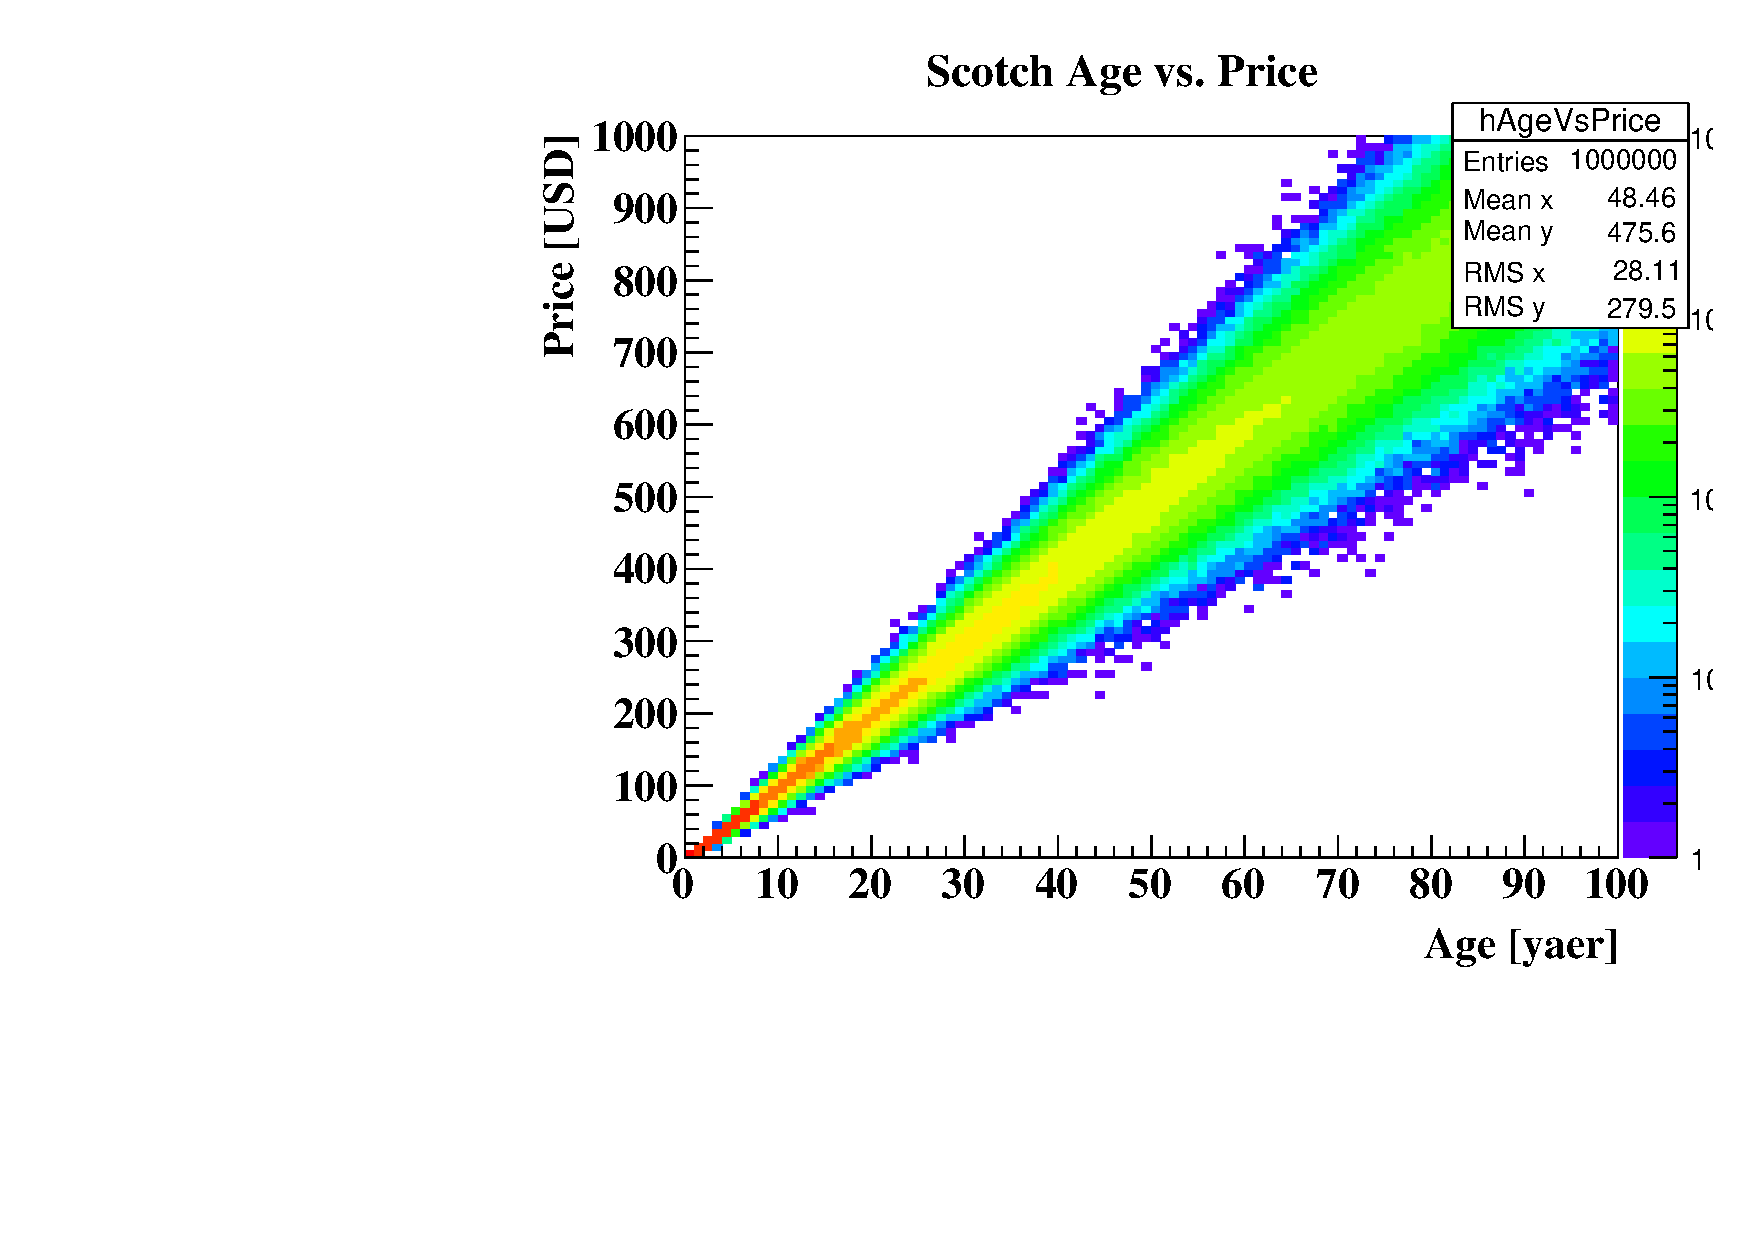
\includegraphics[width=12cm]{./img/ScotchAgeVsPrice.pdf}
\caption{ 
Drawing the age vs. price distribution of {\ttfamily example::Scotch} class from {\ttfamily TTree::Draw}.
}
\end{center}\end{figure}

An example script {\ttfamily mac/example.py} demonstrates how you can:
\begin{itemize}
\item Instantiate {\ttfamily example::Scotch} and save it in a \ROOT file
\item Create a {\ttfamily TTree} of {\ttfamily example::Scotch} for 1e6 entries and save
\item Read-in stored {\ttfamily TTree} and make a very simple access to the stored data product
\item Read-in stored {\ttfamily TTree} and call {\ttfamily TTree::Draw} on the stored data product
\end{itemize}

Note that storing multiple variables into a separate branch of {\ttfamily TTree} (i.e. Ntuple approach)
is much more tedious than storing a class instance as demonstrated in {\ttfamily Scotch::ShipScotch}
function. There, you can find a single line to create a {\ttfamily TTree} branch:
\begin{lstlisting}
tree.Branch("scotch",&data);
\end{lstlisting}
where ``data'' is a {\ttfamily example::Scotch} instance.
With this single line call, all variables in {\ttfamily example::Scotch} instance is stored
with a proper type, and will be readout correctly.

Another myth often people have is that it is very hard to access this object information from
{\ttfamily TTree}. As you can see in the {\ttfamily example.py}, this is completely irrelevant:
you can access the object directly via branch name. A single line in {\ttfamily Python} from
the script is shown below:
\begin{lstlisting}
ch.scotch.Speak()
\end{lstlisting}
which accesses the stored object and calling the class member function {\ttfamily example::Beer::Speak()}.

\subsection{Package Dependency}
The package {\ttfamily Example/Dependent} is prepared to demonstrate how one can make an inter-package 
dependency. In particular, this package depends on {\ttfamily Example/Function} package. Make sure
you have finished building {\ttfamily Example/Function} before building this package.

As you can see in {\ttfamily Stout.h}, the \CPP class {\ttfamily example::Stout} inherits from
{\ttfamily example::Beer}. In order to avoid re-compilation of {\ttfamily example::Beer} class,
we take a usual approach of just {\it linking} the libraries together. Take a look at 
{\ttfamily GNUmakefile}, in particular the following lines:
\begin{lstlisting}
...
INCFLAGS += -I$(LARLITE_USERDEVDIR)/Example
...
LDFLAGS += -L$(LARLITE_LIBDIR) -lExample_Function
\end{lstlisting}
As advertised in the previous section, you must include the path to find {\ttfamily Beer.h} (which
is called from {\ttfamily Stout.h} via {\ttfamily \#include ``Beer.h''}) in {\ttfamily INCFLAGS}, and
both a path and name of a library that contains {\ttfamily example::Beer} class definition in
{\ttfamily LDFLAGS}. 

An example script {\ttfamily mac/example.py} demonstrates an instantiation of {\ttfamily example::Stout}
class and also a call to its base class function {\ttfamily example::Beer::Speak()}.

\subsection{\python in \CPP}
Finally, some users are interested in developing \CPP code to directly operate on \python objects.
An example {\ttfamily Example/PyExample} is prepared to give a tip on how one can write a \CPP
API for \python. This is much better documented as a part of \python documentation:
\begin{center}
{\color{blue}\url{https://docs.python.org/2/c-api/}}
\end{center}

Using a native \python \CPP API is not very easy nor straight forward. Hence in this example,
again, we use \PyROOT binding that makes our life much easier. In short, a difference of two
methods is that you do not have to write your own binding, which is an extra code that has nothing
to do with your algorithm. Finally, that being said, there are other bindings available out there
such as {\ttfamily Cython} (... and \PyROOT uses one of them underneath anyways).

\subsubsection{External Dependnecy}
First of all, you will be using native \python classes, hence you will depend on \python.
Accordingly you have to modify {\ttfamily GNUmakefile}, in particular {\ttfamily INCFLAGS} and
{\ttfamily LDFLAGS}. Notice following 2 lines in {\ttfamily GNUmakefile}:
\begin{lstlisting}
...
INCFLAGS += $(shell python-config --includes)
...
LDFLAGS += $(shell python-config --ldflags)
\end{lstlisting}
each specifying an extra path to find a \python header file and libraries.

\subsubsection{Hiding \python Header From \CINT}
\python header file is called {\ttfamily Python.h}, and is not parse-able via \ROOT \CINT
compiler. So you have to hide it from \CINT dictionary generation step. This can be seen
in {\ttfamily PyExample.h} header file:
\begin{lstlisting}
...
#ifndef __CINT__
// You have to hide native Python header include from CINT                                                                                                                                                  
#include "Python.h"
#endif
...
\end{lstlisting}

You also need to provide two magic lines to forward declare types:
\begin{lstlisting}
...
struct _object;
typedef _object PyObject;
...
\end{lstlisting}
which is for \python generic object pointers to be used (this is a part of \python \CPP API).

\subsubsection{{\ttfamily example::PyExample::Convert}}
The example class {\ttfamily example::PyExample} has an example function to create a
\python list from a \CPP {\ttfamily std::vector<std::string>} object. You can look at the
source code as to how one can do this very simple operation, and take a look at \python
documentation for doing more elaborate operations.

Running {\ttfamily mac/example.py} should show you how this function works.
Obviously you may want to expand the code to work with more advanced \python objects
such as {\ttfamily numpy} array, {\ttfamily matplotlib} axis, and such. The author
does not have much experience to extend too far, but is happy to discuss if you need a help.

\subsection{Documenting Code Using {\ttfamily Doxygen}}
Though this is not everyone's favorite choice, {\ttfamily doxygen} is a popular method to
provide an in-line documentation in the source code. It works pretty nicely with \CPP, and
somewhat at acceptable level with \python. It is the recommended choice for LArSoft to provide
a minimal documentation.

LArLite repositories comes with a doxygen script. You can try generating a documentation
in {\ttfamily Example} directory by typing:
\begin{lstlisting}
  > make doxygen
\end{lstlisting}
({\bf you need doxygen installed in your system!}).

\begin{figure}[htb]\begin{center}
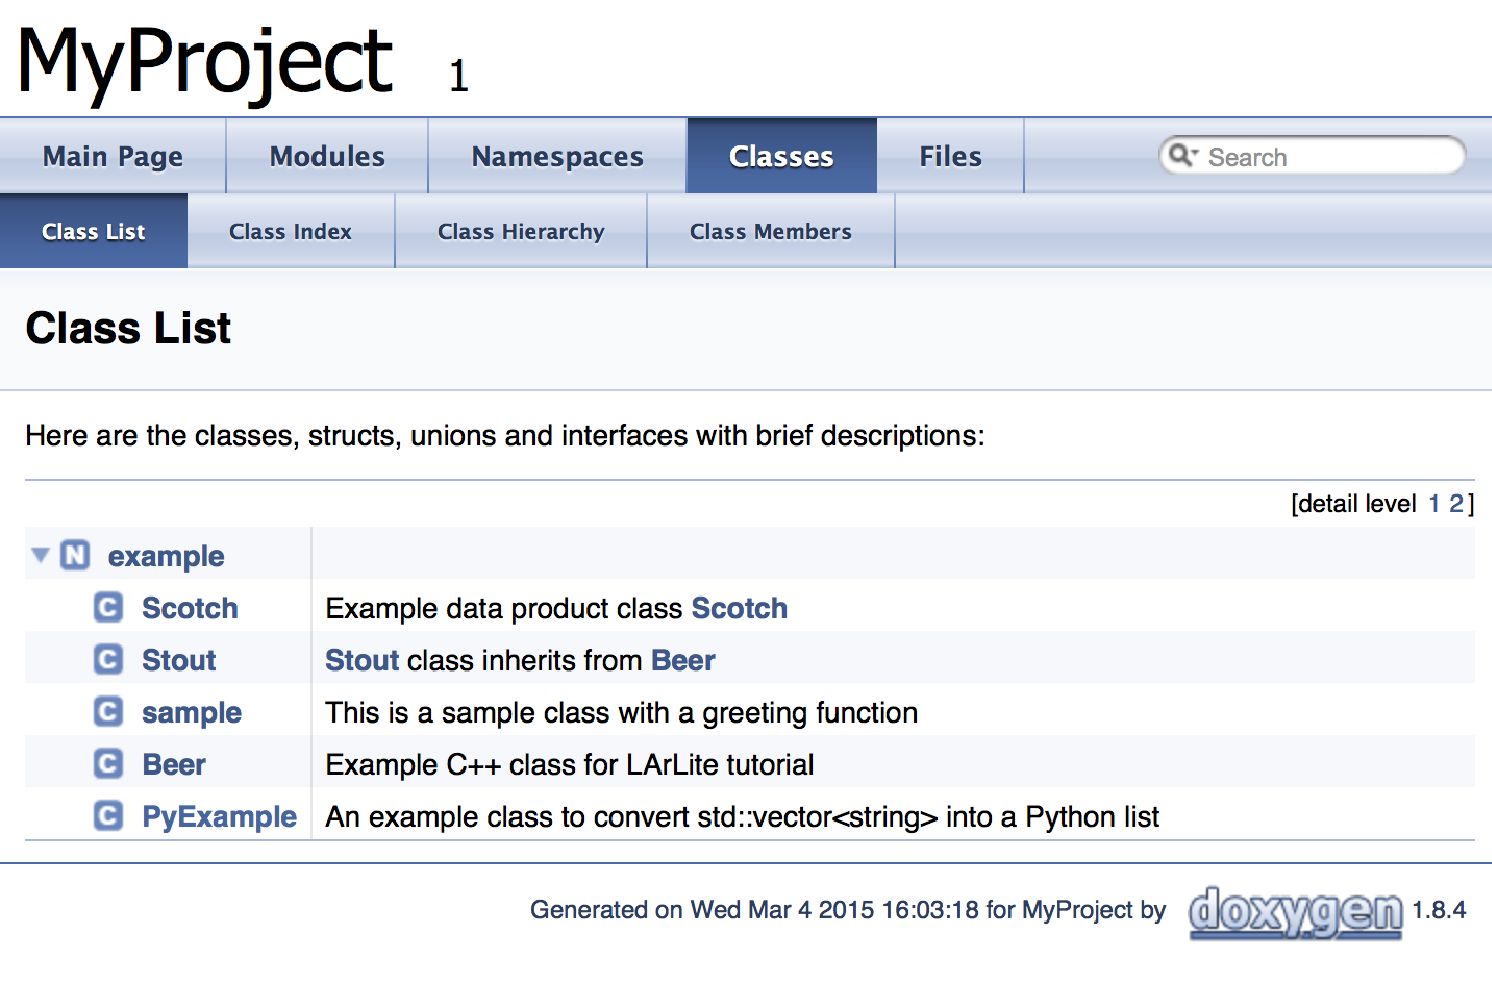
\includegraphics[width=12cm]{./img/doxygen.pdf}
\caption{ 
Doxygen web page generated by ``{\ttfamily make doxygen}'' command for {\ttfamily Example} repository.
}
\end{center}\end{figure}

After successfully running the above command, you should find a chain of HTML files 
to browse through (no internet needed). This way you can also check your doxygen comment
format (whether this is correct or not) before you commit the code. You can look at the
generated documentation using a command like below:
\begin{lstlisting}
  > firefox -a doc/dOxygenMyProject/html/index.html 
\end{lstlisting}
on {\ttfamily Linux} or
\begin{lstlisting}
  > open doc/dOxygenMyProject/html/index.html 
\end{lstlisting}
on {\ttfamily OSX}. The figure shows a generated documentation webpage on the author's laptop.

To understand {\ttfamily doxygen} comment style, refer to their web documentation:
\begin{center}
{\color{blue}\url{http://www.stack.nl/~dimitri/doxygen/manual/docblocks.html}}
\end{center}



% FAQ
\chapter{FAQ}
\label{chap:faq}

This chapter discuss about how to generating user's own code development space.
In particular following itmes are discussed in the respective order.
\begin{itemize}
\item Getting started: your own code repository
\item A simple \CPP project package 
\item Stuffing your package
\begin{itemize}
  \item Simple \CPP class
  \item \anaunit (see Ch.\ref{chap:analysis}).
  \item \ertool algorithm class (see \ertool documentation)
  \item \ertool filter class (see \ertool documentation)
  \item \ertool analysis class (see \ertool documentation)
  \item \CPP functions
\end{itemize}
\item Details: LArLite build basics
\item Advanced Code Development
\begin{itemize}
  \item \CPP functions outside classes
  \item Inter-package dependence
  \item Data product: storing \CPP class instance in \ROOT file
  \item \python in \CPP (i.e. opposite of \PyROOT)
\end{itemize}
\end{itemize}

\section{Creating Your Repository}
\label{sec:devrepo}

LArLite supports user code development under \UserDev.
More precisely, it is assumed to be under any path that is set to the value of shell environment variable {\ttfamily \$LARLITE\_USERDEVDIR}. 
For the sake of simplicity we stick with \UserDev in this section.

\subsection{Note About \UserDev}
Important note first:
\begin{itemize}
  \item {\ttfamily UserDev/GNUmakefile}, if it exists, is generated by setup.sh and it does not belong to LArLite repository (ignore it).
  \item Some sub-directories belong to LArLite (see below). Some of these depend on LArLite and some don't. It is useful to note them briefly here.
    \begin{itemize}
        \item {\ttfamily BasicTool} contains useful packages like {\ttfamily GeoAlgo} and has no dependency outside
        \item {\ttfamily SelectionTool} contains useful packages like {\ttfamily ERTool} and depends on {\ttfamily BasicTool}
        \item {\ttfamily RecoTool} contains shower reconstruction code and depends on {\ttfamily core}
        \item {\ttfamily LArLiteApp} contains LArLite application from {\ttfamily GeoAlgo} and {\ttfamily ERTool} 
    \end{itemize}
  \item You can create new directories under \UserDev and that won't bother other users. We'll do this below. 
  This is all done through {\ttfamily .gitignore} rule placed under the top directory. 
\end{itemize}

These features of \UserDev are there so that you feel more free to make a mess (sorry, I meant, to develop code) there!

\subsection{Creating Your Sub-Repository in \UserDev}
\label{sec:devrepo:makenew}
Obviously I cannot just say ``do whatever under \UserDev'' and leave: I would love to support a very easy way to develop code (or make a mess) under \UserDev. I will just show you how to do things here:
\begin{lstlisting}
     > llgen_repository MyRepo
\end{lstlisting}
where the execution command is an alias explained in Sec.\ref{sec:configure}.
This should create a new directory called {\ttfamily MyRepo} under \UserDev. 
That is your new repository. As said, this does not affect LArLite repository. 
If you don't want to keep {\ttfamily MyRepo}, simply ``{\ttfamily rm -r}'' it.

Another thing to note here: your repository will contain code and you will compile them, making a compiled shared object library. 
Your repository name will be used to name your library file (if you follow LArLite code generation scripts described in the followings). 
So pick a name that suits for your purpose. You do not want to pick a generic name that might coincide with some other libraries on your machine.

\subsection{What's in MyRepo?}

Your new repository comes with a GNUmakefile (which does nothing for now) and {\ttfamily doc} 
directory with a doxygen script but empty otherwise. Under this space, you can create your ``packages'' as a 
set of \CPP code to be compiled into a library. We will discuss about more later.

\subsection{Creating Your Sub-Repository in {\ttfamily github}}
In the previous section, we created a new repository {\ttfamily MyRepo} under \UserDev. But that's just a directory on your laptop, and you may want to keep it as your code repository using either {\ttfamily svn} or {\ttfamily github} (or anything else you would like to use). Here, I briefly mention how you can do this using {\ttfamily github} because it's very easy given that you already have a {\ttfamily github} account.

First of all, go to {\ttfamily github.com} and create your own repository: go to your {\ttfamily github} account web page, and click on ``+'' symbol that is toward right-top of the web page. Choose ``New repository''. Then enter the repository name you are about to create. Ideally you may want to choose a somewhat unique name as described in Sec.\ref{sec:devrepo:makenew}. You can always remove your repository if you don't like it.

Then checkout your empty repository. As an example, I use my empty repo called {\ttfamily EmptyRepo}.
\begin{lstlisting}
    > cd $LARLITE_USERDEVDIR
    > git clone git@github.com:drinkingkazu/EmptyRepo EmptyRepo
\end{lstlisting}
Now simply run:
\begin{lstlisting}
    > python bin/gen_new_repository EmptyRepo
    > cd EmptyRepo
    > git add .
    > git commit -m ``new repository''
    > gitpush -u origin master
\end{lstlisting}
and you are done!
From the next time, if you want to install LArLite from scratch, simply checkout your repository under UserDev with the same name.

As said many times, of course, your repository is independent of LArLite repository.





\section{Creating a Package}
\label{sec:package}
Here, I assume we are working under {\ttfamily UserDev/MyRepo}. 
In fact, since it's tedious, I will just refer to {\ttfamily MyRepo}.

\subsection{What is a ``Package''?}
``Package'' is a directory under a repository that is compiled and generates one {\bf shred object library}
(i.e. a file with {\ttfamily .so} extension). This library is loaded at a run-time or linked via compiler as one byte code file.
This gives you a sense of what to include in one package: having too many classes (and especially unrelated classes) in one package
means an extra overhead cost for a run-time loading or linking at compilation. In other words, you probably do not want make one 
library per class, but also not one library for all classes. A package should contain a group of \CPP classes/functions which you
think it makes sense to put together.

\subsection{Making a Simple \CPP Package}

Like advertised many times, LArLite was originally a \CPP project play ground for summer students. 
The author thinks it's very important to have an empty \CPP package generator that comes with build system, 
so that a user can focus on writing the algorithm instead of figuring out how to compile and such.

So here it is: there is a \python script to generate an empty \CPP package:
\begin{lstlisting}
    $LARLITE_BASEDIR/bin/gen_package
\end{lstlisting}
This script takes one input argument which is used to name a ``package'', a directory to be created under {\ttfamily MyRepo}.
This script {\bf needs to be executed somewhere under {\ttfamily MyRepo}} (otherwise you'll see an error message).
One can run this script via alias:
\begin{lstlisting}
    > llgen_package MyProject
\end{lstlisting}
which will create a directory {\ttfamily MyRepo/MyProject} that include minimal set of source codes to compile an empty \CPP class. 
You can have your name choice in place of ``MyProject''. After running the command, try:
\begin{lstlisting}
    > cd MyProject
    > make -j4
\end{lstlisting}
This compiles your code and makes {\ttfamily libMyRepo\_MyProject.so} under {\ttfamily lib} directory.
What you compiled is a \CPP class called ``sample'' defined in {\ttfamily sample.h}. 


\subsection{Using in Interpreter}

So how can you ``use'' this \CPP class? You can write a binary executable code, or try out in \CINT or \PyROOT. Here is an example:
\begin{lstlisting}
    > root
    root[0] sample k;
\end{lstlisting}
Above lines work (i.e. your class instance is created) because \CINT is informed about your class. 

\subsection{``Hello World'' Development}
\label{sec:helloworld}
Let's try a simple modification to your class. Here's an example ``hello world'' program using \CPP class. Open {\ttfamily sample.h} and add a {\ttfamily void} function as shown below:
\begin{lstlisting}
class sample{
public:
  /// Default constructor
  sample(){};
  /// Default destructor
  virtual ~sample(){};
  /// Hello world!
  void HelloWorld() { std::cout << ``Hello World!'' << std::endl; }
};
\end{lstlisting}
Save, close and compile (i.e. type ``make''). Now, try the following in \CINT or \PyROOT:
\begin{lstlisting}
    > root
    root[0] sample k;
    root[1] k.HelloWorld();
    Hello World!
    root[2]
\end{lstlisting}

Whenever you want to start a new project with an empty class, you can come back to this example and create your new \CPP project!





\section{Adding Basic \CPP Classes}
\label{sec:expand_package}

As discussed in the previous section, one should populate a package with a group of \CPP classes.
This section describes how to add various types of \CPP classes to your package.

\subsection{Simple \CPP Class}
Sometimes (rather often) you want to generate a completely generic \CPP class for very good reasons: to develop 
some algorithm that is independent of the framework (= easy portability to outside LArLite).

Here is a script for you:
\begin{lstlisting}
    > cd $LARLITE_USERDEVDIR/MyRepo/MyProject
    > llgen_class_empty MyEmptyClass
\end{lstlisting}
Now you should see {\ttfamily MyEmptyClass.h} and {\ttfamily MyEmptyClass.cxx} created under {\ttfamily MyAna}
package. There also made appropriate modification to {\ttfamily LinkDef.h} so that you can just type:
\begin{lstlisting}
    > make -j2
\end{lstlisting}
to compile your new class. Now develop your awesome algorithm and make it a non-empty class ;)

\subsection{\anaunit Class}
If you wish to generate an empty \anaunit class code (to be implemented by you), simply try:
\begin{lstlisting}
    > cd $LARLITE_USERDEVDIR/MyRepo/MyProject
    > llgen_class_anaunit MyAna
\end{lstlisting}

Executing above commands create {\ttfamily MyAna.cxx} and {\ttfamily MyAna.h} (and an appropriate modification to {\ttfamily LinkDef.h}).
Try:
\begin{lstlisting}
    > make -j4
\end{lstlisting}
You just made your new \anaunit class, {\ttfamily MyAna}, whieh inherits from {\ttfamily ana\_base}! 
Your new \anaunit is accessible from \CINT or \PyROOT like any other classes in LArLite:
\begin{lstlisting}
    > root
    root[0] larlite::MyAna my_ana_instance
\end{lstlisting}
Now go ahead and code up this analysis unit, and run with {\ttfamily ana\_processor}! 

\subsubsection{Run Your Analysis Unit: \PyROOT}
\label{sec:yourrunscript}
There is an example \python run script for \anaunit under {\ttfamily mac} directory, called 
{\ttfamily example\_anaunit.py}. You need a LArLite sample \ROOT file to run this program. 
If you have a sample file, say {\ttfamily trial.root}, you can run the program as follows.
\begin{lstlisting}
    > python mac/example_anaunit.py trial.root
\end{lstlisting}

\subsection{\ertool Classes}
Just as we exercised how to add a new \CPP class to a package, there's analogous python scripts to
generate \ertool reconstruction algorithm, filter, and analysis class:
\begin{lstlisting}
    > cd $LARLITE_USERDEVDIR/MyRepo/MyProject
    > llgen_class_erfilter Trial
    > llgen_class_eralgo Trial
    > llgen_class_erana Trial
\end{lstlisting}
Above three commands generate three \CPP classes: {\ttfamily ERFilterTrial}, {\ttfamily ERAlgoTrial}, and {\ttfamily ERAnaTrial}.
These are implementation of base classes defined in \ertool, hence must be used with {\ttfamily ertool::Manager}.
For details, see \ertool documentation (which is to come...)






\section{Understanding the Build}
\label{sec:build_package}
This section covers the basics of how the LArLite build works, aiming to reduce a black-box content for users and developers.
The following topics are ordered such that a topic of interest to more people gets covered first.

\subsection{{\ttfamily Compiler} and {\ttfamily Linker} for Dummies}
Skip if you already know about them, obviously.

Our \CPP source codes are merely descriptions of what we want our computer to do in human-friendly language 
(disagree on ``human-fiendly''? Welcome to the club).
A {\ttfamily compiler} takes in our source code and generate a machine-friendly description, often called as an {\it object file} or {\it byte code}.
When you compile your package in LArLite, you find files with {\ttfamily .o} extension: these are the object files.

Now having many granular object files is not very helpful.
A {\ttfamily linker} allows us to combine multiple object files and create a {\it shared object library} file.
You find such files with {\ttfamily .so} extension under {\ttfamily \$LARLITE\_LIBDIR} if you compiled any package.
The scope of what objects should be put together is really a developer's choice.
In LArLite, this is done per package.
Another (and more important) advantage of shared object libraries kicks in when you compile another code that depends on it.
Say you have a \CPP class {\ttfamily A} and {\ttfamily B} where {\ttfamily B} depends on {\ttfamily A}. 
Once you have {\ttfamily A} compiled with {\ttfamily .so} file, a separate compilation of {\ttfamily B} does not require
a re-compilation of {\ttfamily A}'s source code. Instead, you can {\it link} the {\ttfamily A}'s library upon compilation
of {\ttfamily B}'s library.

In LArLite, we compile files with {\ttfamily .cxx} extensions with a compiler, and create a shared object library using a linker, which
is nothing special compared to any other softwares' build system.

\subsection{{\ttfamily INCFLAGS} and {\ttfamily LDFLAGS}: LArLite Compiler Flags}
In LArLite package's {\ttfamily GNUmakefile}, you may see variables named as {\ttfamily INCFLAGS} and {\ttfamily LDFLAGS} where
the latter may not appear in some simple code packages (i.e. don't worry about not seeing {\ttfamily LDFLAGS} in your {\ttfamily GNUmakefile}).
These are called {\it compiler flags} and passed onto a compiler and linker respectively.

\subsubsection{INCFLAGS}
{\ttfamily INCFLAGS} is used by a compiler to search for files you specify with {\ttfamily \#include} preprocessor command in your source code.
In other words, if your source code calls {\ttfamily \#include <TH1D.h>}, then the directory path which contains {\ttfamily TH1D.h} has to be
added to {\ttfamily INCFLAGS}. The format of {\ttfamily INCFLAGS} is ``-I\$PATH'' where you should replace ``\$PATH'' with the relevant
directory path.

That being said, by default, LArLite includes a \ROOT's include flags.
\ROOT follows a standard method to provide such flags, and you can try this in your installation as well:
\begin{lstlisting}
  > root-config --cflags
\end{lstlisting}
The output of above command is a part of LArLite's default {\ttfamily INCFLAGS}.

\subsubsection{LDFLAGS}
{\ttfamily LDFLAGS} is used by a linker to find libraries to be linked into your package. If your package depends on any externaly compiled
code, for instance a \ROOT class {\ttfamily TH1D}, you have to specify the library to be linked here. The format is 
{\ttfamily -L\$PATH -l\$LIBNAME} where ``\$PATH'' is the directory path that contains a library named ``lib\$LIBNAME.so''. Note that
you should exclude the prefix ``lib'' when you specify it in {\ttfamily LDFLAGS} as that is the standard of how a linker takes in library names.

The default flags in LArLite includes a \ROOT's library flags.
Again, as it was the case for {\ttfamily INCFLAGS}, you can try:
\begin{lstlisting}
  > root-config --libs
\end{lstlisting}
which include most of standard \ROOT libraries such as IO, histogram, TTree, TMatrix, TVector3, etc.

\subsubsection{Flags for LArLite Packages}
You may write a package that depends on existing LArLite code.
One example is an analysis code that inherits from {\ttfamily lalrite::ana\_base}. 
Then you will have to specify {\ttfamily INCFLAGS} and {\ttfamily LDFLAGS}.

Specifying every single {\ttfamily INCFLAGS} and {\ttfamily LDFLAGS} for LArLite code is definitely annoying.
So we follow the popular standard and the following scripts are prepared:
\begin{itemize}
\item {\ttfamily larlite-config} for LArLite's analysis framework
\item {\ttfamily basictool-config} for code under \UserDev/BasicTool 
\item {\ttfamily seltool-config} for code under \UserDev/SelectionTool
\item {\ttfamily recotool-config} for code under \UserDev/RecoTool
\end{itemize}
These scripts can be run with either {\ttfamily --includes} or {\ttfamily --libs} option, and they
simply prints out relevant string to be added to {\ttfamily INCFLAGS} and {\ttfamily LDFLAGS} respectively.
For instance, you may try:
\begin{lstlisting}
  INCFLAGS += $(shell larlite-config --includes)
\end{lstlisting}
and/or
\begin{lstlisting}
  LDFLAGS += $(shell larlite-config --libs)
\end{lstlisting}
in your {\ttfamily GNUmakefile}.

If you use {\ttfamily gen\_class\_anaunit} or similar script, actually, this modification to a {\ttfamily GNUmakefile} is done
by the same script. Hence you do not need to worry about it.

\subsection{Compiler \& Linker Used by LArLite}
Let me make a brief note on how compiler/linker is picked and what default compiler/linker flags are set for LArLite build.

When possible LArLite attempts to use \clang++. In particular this is searched and set when one runs {\ttfamily setup.sh} script.
The configured compiler name is set to a shell environment variable {\ttfamily \$LARLITE\_CXX}.
Further, compiler/linker specific flags are defined in:
\begin{lstlisting}
  > $LARLITE_BASEDIR/Makefile/Makefile.X
\end{lstlisting}
where {\ttfamily X} may be either ``Darwin'' or ``Linux''. 


\section{Advanced Development}
\label{sec:advanced_package}

In this section we follow a prepared example that can be found in:
\begin{center}
{\color{blue}\url{https://github.com/drinkingkazu/Example}}
\end{center}
You might have already checked out this repository as this was mentioned briefly
in the introductory section (see Sec.\ref{sec:build}). 
If not, can certainly checkout under \UserDev:
\begin{lstlisting}
  > cd $LARLITE_USERDEVDIR
  > git clone https://github.com/drinkingkazu/Example
\end{lstlisting}

This repository contains following packages:
\begin{itemize}
\item {\ttfamily Empty} for the simplest example to introduce a simple \CPP class
\item {\ttfamily Function} for demonstrating a \CPP function to be exported into a dictionary
\item {\ttfamily Dependent} for showing how to make inter-package dependencies
\item {\ttfamily DataProduct} as an example of how to store a class instance into a file
\end{itemize}
where we skip the first item, {\ttfamily Empty}, as that has been covered in the previous section.

\subsection{\CPP Functions}
I would like to avoid a confusion: \CPP class is an extension of data structure. In particular,
you do not have to make \CPP class for inventing one or a few functions. Just like we have done
some practice with \CPP class, it would be useful to have \CPP functions in a dictionary.
The point of this package is to show how one can do this.

Take a look at {\ttfamily MyFunctions.h} and {\ttfamily MyFunctions.cxx} source code: there, I defined
functions:
\begin{lstlisting}
  void hello_world();
  Beer Brew(const int age);
\end{lstlisting}
where {\ttfamily example::Beer} is a \CPP class defined in {\ttfamily Beer.h}: it's very very simple class for
playing around unlike the sophisticated name.

Now a compilation works just as expected, and there is nothing special about these functions.
What you may find useful is a format to declare above functions in {\ttfamily LinkDef.h}:
\begin{lstlisting}
#pragma link C++ function  example::hello_world()+;
#pragma link C++ function  example::Brew(const int)+;
\end{lstlisting}
As you can see, a) you do not specify the return type of the function, and b) you only need to specify
the argument types. 

You can try executing an example script {\ttfamily mac/example.py} which calls those functions. 
Take a look at the script's contents and see if that makes sense (... and ask a question if you have any!).
{\color{red}\bf There is one caveat}, however: currently \ROOT seems to require \CPP class compiled
in the same library to be instantiated {\bf before} \CPP functions to be called. The author will
open a ticket for this to be fixed.

\subsection{\ROOT Data Product Class}
Once you get familiar with all LArLite features, you might want to store \CPP object in a file
as a {\ttfamily data product}. The easiest (and recommended) method is to use a \ROOT file.
A rule of the thumb is that any \CPP class that is generated with a \ROOT {\it dictionary} can
be stored in a \ROOT file. You can find details in the \ROOT manual.

If you use LArLite as your code development environment, \ROOT dictionary file is always
generated and built at compilation stage of your package. 

An example can be found in the package {\ttfamily DataProduct}.
There, a data product class called {\ttfamily example::Scotch} is defined. 

\begin{figure}[htb]\begin{center}
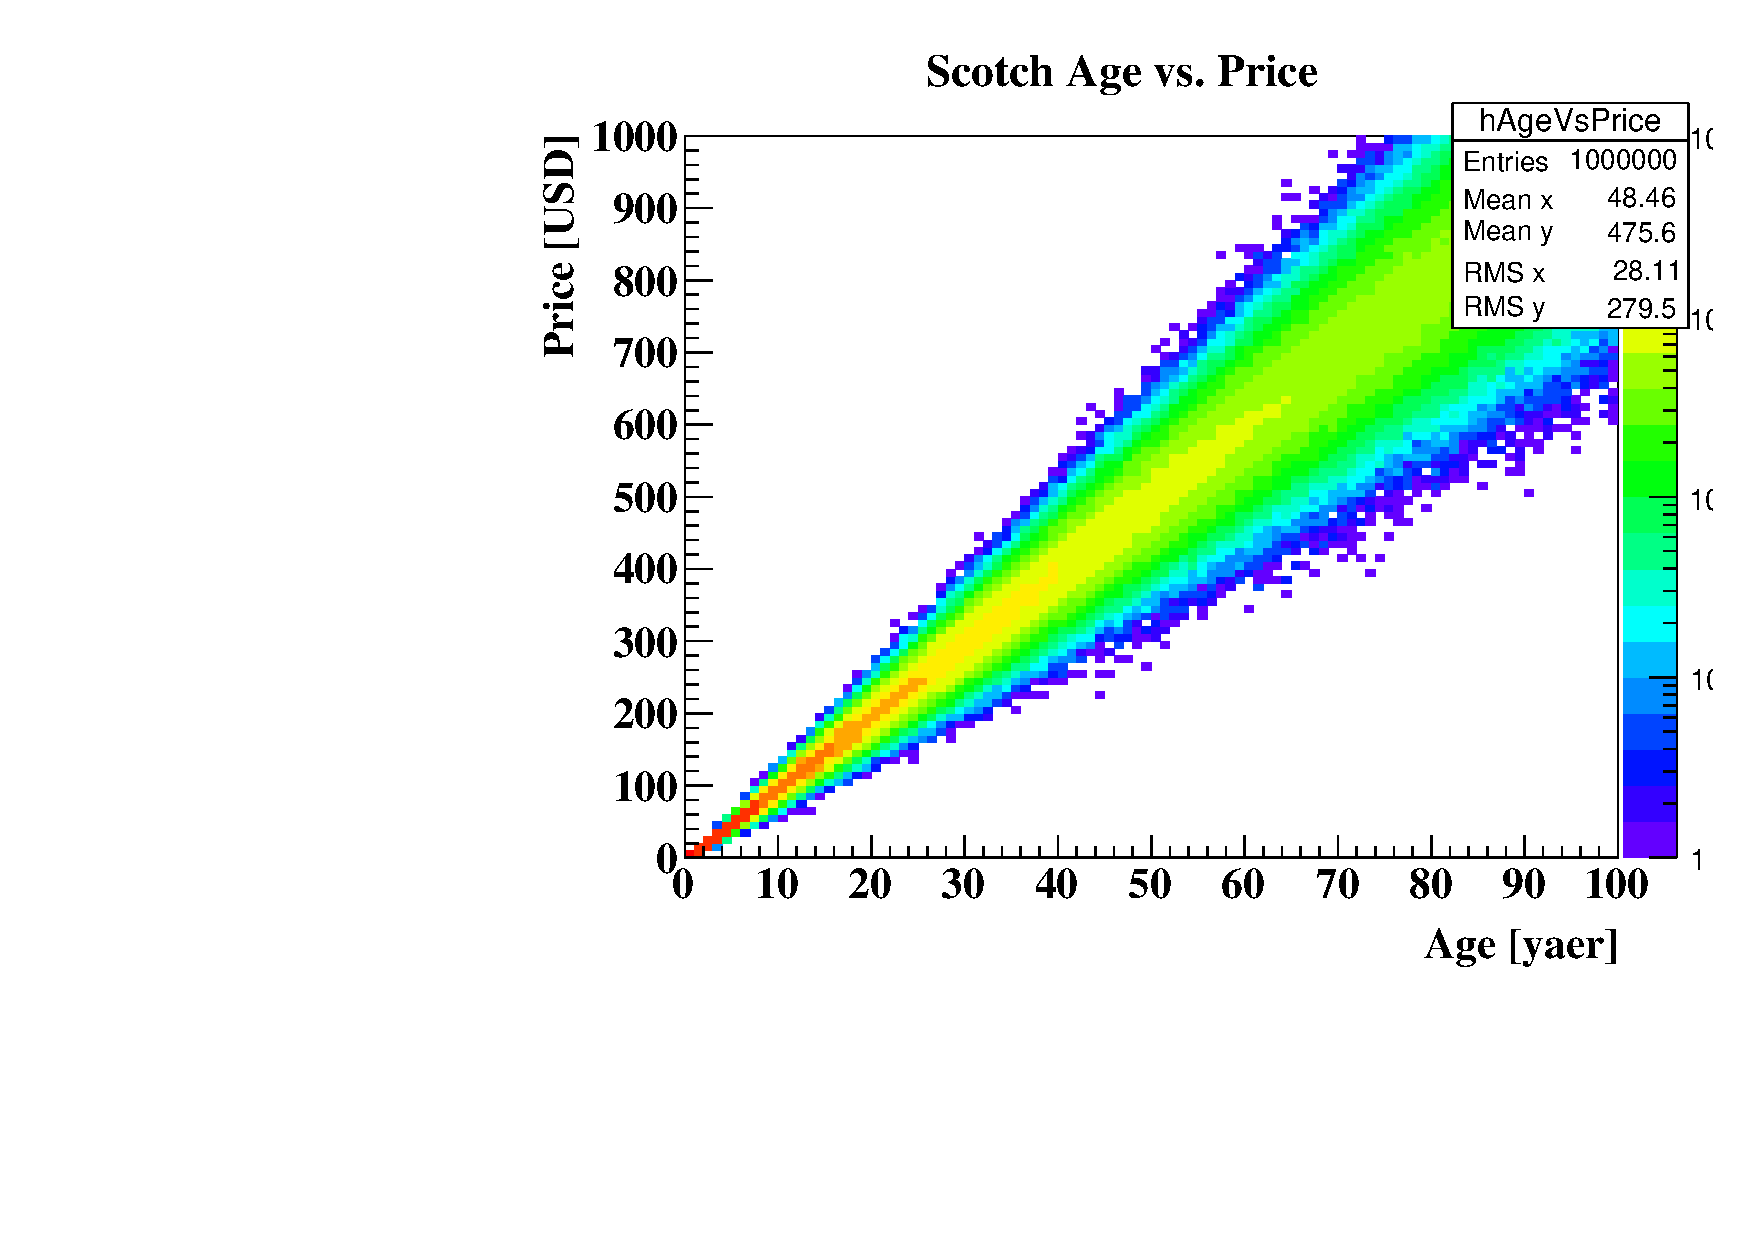
\includegraphics[width=12cm]{./img/ScotchAgeVsPrice.pdf}
\caption{ 
Drawing the age vs. price distribution of {\ttfamily example::Scotch} class from {\ttfamily TTree::Draw}.
}
\end{center}\end{figure}

An example script {\ttfamily mac/example.py} demonstrates how you can:
\begin{itemize}
\item Instantiate {\ttfamily example::Scotch} and save it in a \ROOT file
\item Create a {\ttfamily TTree} of {\ttfamily example::Scotch} for 1e6 entries and save
\item Read-in stored {\ttfamily TTree} and make a very simple access to the stored data product
\item Read-in stored {\ttfamily TTree} and call {\ttfamily TTree::Draw} on the stored data product
\end{itemize}

Note that storing multiple variables into a separate branch of {\ttfamily TTree} (i.e. Ntuple approach)
is much more tedious than storing a class instance as demonstrated in {\ttfamily Scotch::ShipScotch}
function. There, you can find a single line to create a {\ttfamily TTree} branch:
\begin{lstlisting}
tree.Branch("scotch",&data);
\end{lstlisting}
where ``data'' is a {\ttfamily example::Scotch} instance.
With this single line call, all variables in {\ttfamily example::Scotch} instance is stored
with a proper type, and will be readout correctly.

Another myth often people have is that it is very hard to access this object information from
{\ttfamily TTree}. As you can see in the {\ttfamily example.py}, this is completely irrelevant:
you can access the object directly via branch name. A single line in {\ttfamily Python} from
the script is shown below:
\begin{lstlisting}
ch.scotch.Speak()
\end{lstlisting}
which accesses the stored object and calling the class member function {\ttfamily example::Beer::Speak()}.

\subsection{Package Dependency}
The package {\ttfamily Example/Dependent} is prepared to demonstrate how one can make an inter-package 
dependency. In particular, this package depends on {\ttfamily Example/Function} package. Make sure
you have finished building {\ttfamily Example/Function} before building this package.

As you can see in {\ttfamily Stout.h}, the \CPP class {\ttfamily example::Stout} inherits from
{\ttfamily example::Beer}. In order to avoid re-compilation of {\ttfamily example::Beer} class,
we take a usual approach of just {\it linking} the libraries together. Take a look at 
{\ttfamily GNUmakefile}, in particular the following lines:
\begin{lstlisting}
...
INCFLAGS += -I$(LARLITE_USERDEVDIR)/Example
...
LDFLAGS += -L$(LARLITE_LIBDIR) -lExample_Function
\end{lstlisting}
As advertised in the previous section, you must include the path to find {\ttfamily Beer.h} (which
is called from {\ttfamily Stout.h} via {\ttfamily \#include ``Beer.h''}) in {\ttfamily INCFLAGS}, and
both a path and name of a library that contains {\ttfamily example::Beer} class definition in
{\ttfamily LDFLAGS}. 

An example script {\ttfamily mac/example.py} demonstrates an instantiation of {\ttfamily example::Stout}
class and also a call to its base class function {\ttfamily example::Beer::Speak()}.

\subsection{\python in \CPP}
Finally, some users are interested in developing \CPP code to directly operate on \python objects.
An example {\ttfamily Example/PyExample} is prepared to give a tip on how one can write a \CPP
API for \python. This is much better documented as a part of \python documentation:
\begin{center}
{\color{blue}\url{https://docs.python.org/2/c-api/}}
\end{center}

Using a native \python \CPP API is not very easy nor straight forward. Hence in this example,
again, we use \PyROOT binding that makes our life much easier. In short, a difference of two
methods is that you do not have to write your own binding, which is an extra code that has nothing
to do with your algorithm. Finally, that being said, there are other bindings available out there
such as {\ttfamily Cython} (... and \PyROOT uses one of them underneath anyways).

\subsubsection{External Dependnecy}
First of all, you will be using native \python classes, hence you will depend on \python.
Accordingly you have to modify {\ttfamily GNUmakefile}, in particular {\ttfamily INCFLAGS} and
{\ttfamily LDFLAGS}. Notice following 2 lines in {\ttfamily GNUmakefile}:
\begin{lstlisting}
...
INCFLAGS += $(shell python-config --includes)
...
LDFLAGS += $(shell python-config --ldflags)
\end{lstlisting}
each specifying an extra path to find a \python header file and libraries.

\subsubsection{Hiding \python Header From \CINT}
\python header file is called {\ttfamily Python.h}, and is not parse-able via \ROOT \CINT
compiler. So you have to hide it from \CINT dictionary generation step. This can be seen
in {\ttfamily PyExample.h} header file:
\begin{lstlisting}
...
#ifndef __CINT__
// You have to hide native Python header include from CINT                                                                                                                                                  
#include "Python.h"
#endif
...
\end{lstlisting}

You also need to provide two magic lines to forward declare types:
\begin{lstlisting}
...
struct _object;
typedef _object PyObject;
...
\end{lstlisting}
which is for \python generic object pointers to be used (this is a part of \python \CPP API).

\subsubsection{{\ttfamily example::PyExample::Convert}}
The example class {\ttfamily example::PyExample} has an example function to create a
\python list from a \CPP {\ttfamily std::vector<std::string>} object. You can look at the
source code as to how one can do this very simple operation, and take a look at \python
documentation for doing more elaborate operations.

Running {\ttfamily mac/example.py} should show you how this function works.
Obviously you may want to expand the code to work with more advanced \python objects
such as {\ttfamily numpy} array, {\ttfamily matplotlib} axis, and such. The author
does not have much experience to extend too far, but is happy to discuss if you need a help.

\subsection{Documenting Code Using {\ttfamily Doxygen}}
Though this is not everyone's favorite choice, {\ttfamily doxygen} is a popular method to
provide an in-line documentation in the source code. It works pretty nicely with \CPP, and
somewhat at acceptable level with \python. It is the recommended choice for LArSoft to provide
a minimal documentation.

LArLite repositories comes with a doxygen script. You can try generating a documentation
in {\ttfamily Example} directory by typing:
\begin{lstlisting}
  > make doxygen
\end{lstlisting}
({\bf you need doxygen installed in your system!}).

\begin{figure}[htb]\begin{center}
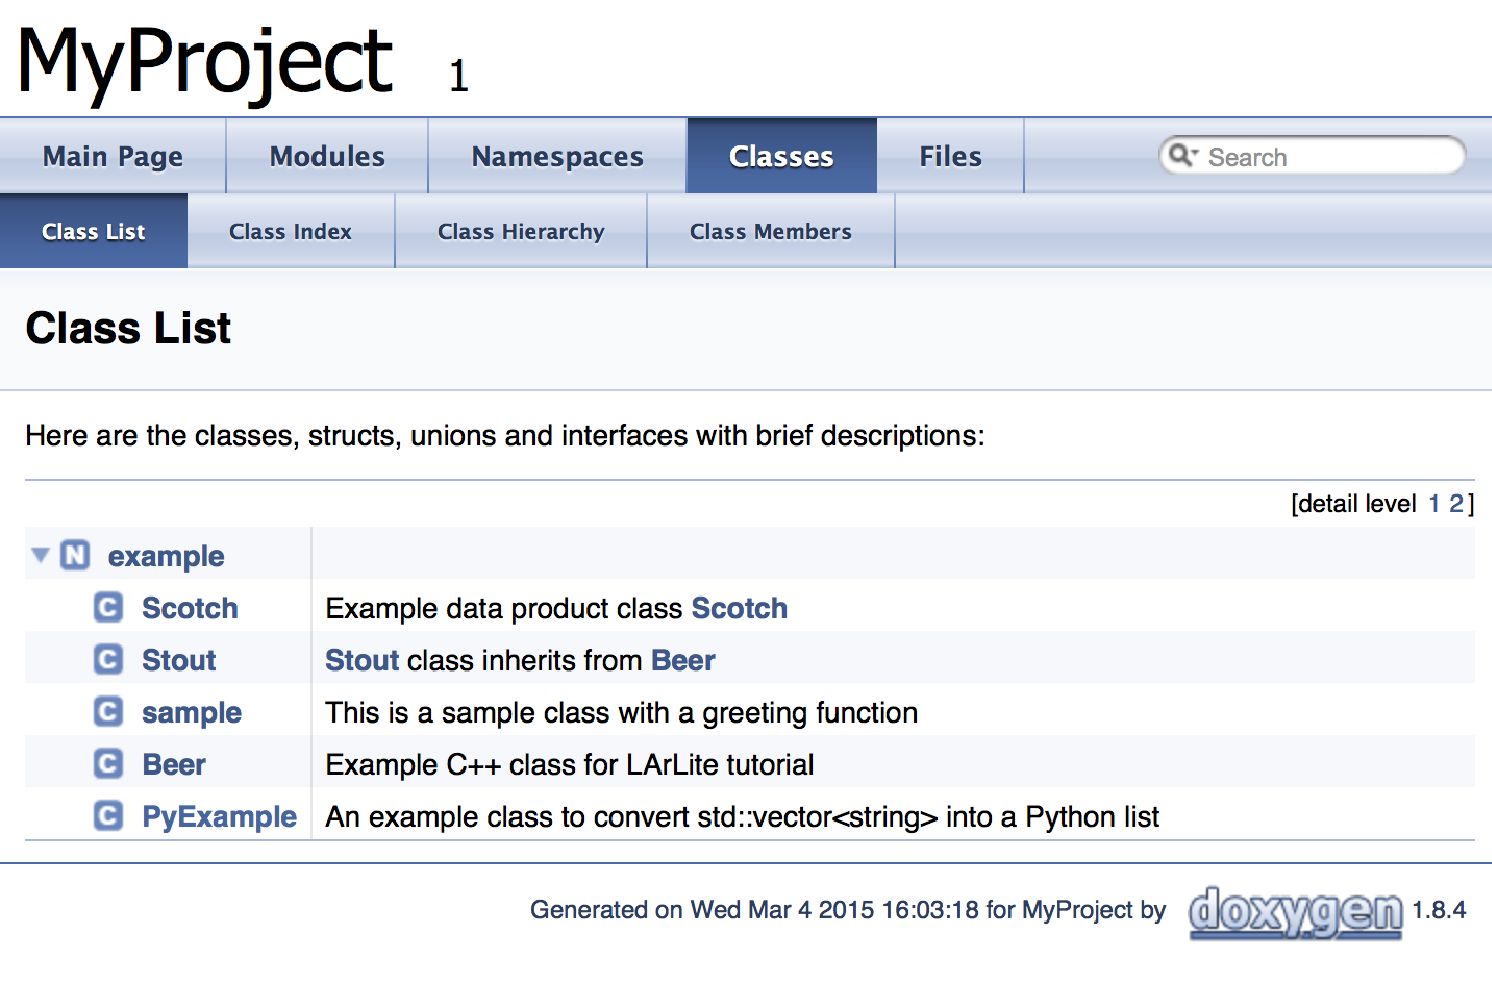
\includegraphics[width=12cm]{./img/doxygen.pdf}
\caption{ 
Doxygen web page generated by ``{\ttfamily make doxygen}'' command for {\ttfamily Example} repository.
}
\end{center}\end{figure}

After successfully running the above command, you should find a chain of HTML files 
to browse through (no internet needed). This way you can also check your doxygen comment
format (whether this is correct or not) before you commit the code. You can look at the
generated documentation using a command like below:
\begin{lstlisting}
  > firefox -a doc/dOxygenMyProject/html/index.html 
\end{lstlisting}
on {\ttfamily Linux} or
\begin{lstlisting}
  > open doc/dOxygenMyProject/html/index.html 
\end{lstlisting}
on {\ttfamily OSX}. The figure shows a generated documentation webpage on the author's laptop.

To understand {\ttfamily doxygen} comment style, refer to their web documentation:
\begin{center}
{\color{blue}\url{http://www.stack.nl/~dimitri/doxygen/manual/docblocks.html}}
\end{center}



\chapter{Releases}
\label{chap:releases}

This chapter discuss about how to generating user's own code development space.
In particular following itmes are discussed in the respective order.
\begin{itemize}
\item Getting started: your own code repository
\item A simple \CPP project package 
\item Stuffing your package
\begin{itemize}
  \item Simple \CPP class
  \item \anaunit (see Ch.\ref{chap:analysis}).
  \item \ertool algorithm class (see \ertool documentation)
  \item \ertool filter class (see \ertool documentation)
  \item \ertool analysis class (see \ertool documentation)
  \item \CPP functions
\end{itemize}
\item Details: LArLite build basics
\item Advanced Code Development
\begin{itemize}
  \item \CPP functions outside classes
  \item Inter-package dependence
  \item Data product: storing \CPP class instance in \ROOT file
  \item \python in \CPP (i.e. opposite of \PyROOT)
\end{itemize}
\end{itemize}

\section{Creating Your Repository}
\label{sec:devrepo}

LArLite supports user code development under \UserDev.
More precisely, it is assumed to be under any path that is set to the value of shell environment variable {\ttfamily \$LARLITE\_USERDEVDIR}. 
For the sake of simplicity we stick with \UserDev in this section.

\subsection{Note About \UserDev}
Important note first:
\begin{itemize}
  \item {\ttfamily UserDev/GNUmakefile}, if it exists, is generated by setup.sh and it does not belong to LArLite repository (ignore it).
  \item Some sub-directories belong to LArLite (see below). Some of these depend on LArLite and some don't. It is useful to note them briefly here.
    \begin{itemize}
        \item {\ttfamily BasicTool} contains useful packages like {\ttfamily GeoAlgo} and has no dependency outside
        \item {\ttfamily SelectionTool} contains useful packages like {\ttfamily ERTool} and depends on {\ttfamily BasicTool}
        \item {\ttfamily RecoTool} contains shower reconstruction code and depends on {\ttfamily core}
        \item {\ttfamily LArLiteApp} contains LArLite application from {\ttfamily GeoAlgo} and {\ttfamily ERTool} 
    \end{itemize}
  \item You can create new directories under \UserDev and that won't bother other users. We'll do this below. 
  This is all done through {\ttfamily .gitignore} rule placed under the top directory. 
\end{itemize}

These features of \UserDev are there so that you feel more free to make a mess (sorry, I meant, to develop code) there!

\subsection{Creating Your Sub-Repository in \UserDev}
\label{sec:devrepo:makenew}
Obviously I cannot just say ``do whatever under \UserDev'' and leave: I would love to support a very easy way to develop code (or make a mess) under \UserDev. I will just show you how to do things here:
\begin{lstlisting}
     > llgen_repository MyRepo
\end{lstlisting}
where the execution command is an alias explained in Sec.\ref{sec:configure}.
This should create a new directory called {\ttfamily MyRepo} under \UserDev. 
That is your new repository. As said, this does not affect LArLite repository. 
If you don't want to keep {\ttfamily MyRepo}, simply ``{\ttfamily rm -r}'' it.

Another thing to note here: your repository will contain code and you will compile them, making a compiled shared object library. 
Your repository name will be used to name your library file (if you follow LArLite code generation scripts described in the followings). 
So pick a name that suits for your purpose. You do not want to pick a generic name that might coincide with some other libraries on your machine.

\subsection{What's in MyRepo?}

Your new repository comes with a GNUmakefile (which does nothing for now) and {\ttfamily doc} 
directory with a doxygen script but empty otherwise. Under this space, you can create your ``packages'' as a 
set of \CPP code to be compiled into a library. We will discuss about more later.

\subsection{Creating Your Sub-Repository in {\ttfamily github}}
In the previous section, we created a new repository {\ttfamily MyRepo} under \UserDev. But that's just a directory on your laptop, and you may want to keep it as your code repository using either {\ttfamily svn} or {\ttfamily github} (or anything else you would like to use). Here, I briefly mention how you can do this using {\ttfamily github} because it's very easy given that you already have a {\ttfamily github} account.

First of all, go to {\ttfamily github.com} and create your own repository: go to your {\ttfamily github} account web page, and click on ``+'' symbol that is toward right-top of the web page. Choose ``New repository''. Then enter the repository name you are about to create. Ideally you may want to choose a somewhat unique name as described in Sec.\ref{sec:devrepo:makenew}. You can always remove your repository if you don't like it.

Then checkout your empty repository. As an example, I use my empty repo called {\ttfamily EmptyRepo}.
\begin{lstlisting}
    > cd $LARLITE_USERDEVDIR
    > git clone git@github.com:drinkingkazu/EmptyRepo EmptyRepo
\end{lstlisting}
Now simply run:
\begin{lstlisting}
    > python bin/gen_new_repository EmptyRepo
    > cd EmptyRepo
    > git add .
    > git commit -m ``new repository''
    > gitpush -u origin master
\end{lstlisting}
and you are done!
From the next time, if you want to install LArLite from scratch, simply checkout your repository under UserDev with the same name.

As said many times, of course, your repository is independent of LArLite repository.





\section{Creating a Package}
\label{sec:package}
Here, I assume we are working under {\ttfamily UserDev/MyRepo}. 
In fact, since it's tedious, I will just refer to {\ttfamily MyRepo}.

\subsection{What is a ``Package''?}
``Package'' is a directory under a repository that is compiled and generates one {\bf shred object library}
(i.e. a file with {\ttfamily .so} extension). This library is loaded at a run-time or linked via compiler as one byte code file.
This gives you a sense of what to include in one package: having too many classes (and especially unrelated classes) in one package
means an extra overhead cost for a run-time loading or linking at compilation. In other words, you probably do not want make one 
library per class, but also not one library for all classes. A package should contain a group of \CPP classes/functions which you
think it makes sense to put together.

\subsection{Making a Simple \CPP Package}

Like advertised many times, LArLite was originally a \CPP project play ground for summer students. 
The author thinks it's very important to have an empty \CPP package generator that comes with build system, 
so that a user can focus on writing the algorithm instead of figuring out how to compile and such.

So here it is: there is a \python script to generate an empty \CPP package:
\begin{lstlisting}
    $LARLITE_BASEDIR/bin/gen_package
\end{lstlisting}
This script takes one input argument which is used to name a ``package'', a directory to be created under {\ttfamily MyRepo}.
This script {\bf needs to be executed somewhere under {\ttfamily MyRepo}} (otherwise you'll see an error message).
One can run this script via alias:
\begin{lstlisting}
    > llgen_package MyProject
\end{lstlisting}
which will create a directory {\ttfamily MyRepo/MyProject} that include minimal set of source codes to compile an empty \CPP class. 
You can have your name choice in place of ``MyProject''. After running the command, try:
\begin{lstlisting}
    > cd MyProject
    > make -j4
\end{lstlisting}
This compiles your code and makes {\ttfamily libMyRepo\_MyProject.so} under {\ttfamily lib} directory.
What you compiled is a \CPP class called ``sample'' defined in {\ttfamily sample.h}. 


\subsection{Using in Interpreter}

So how can you ``use'' this \CPP class? You can write a binary executable code, or try out in \CINT or \PyROOT. Here is an example:
\begin{lstlisting}
    > root
    root[0] sample k;
\end{lstlisting}
Above lines work (i.e. your class instance is created) because \CINT is informed about your class. 

\subsection{``Hello World'' Development}
\label{sec:helloworld}
Let's try a simple modification to your class. Here's an example ``hello world'' program using \CPP class. Open {\ttfamily sample.h} and add a {\ttfamily void} function as shown below:
\begin{lstlisting}
class sample{
public:
  /// Default constructor
  sample(){};
  /// Default destructor
  virtual ~sample(){};
  /// Hello world!
  void HelloWorld() { std::cout << ``Hello World!'' << std::endl; }
};
\end{lstlisting}
Save, close and compile (i.e. type ``make''). Now, try the following in \CINT or \PyROOT:
\begin{lstlisting}
    > root
    root[0] sample k;
    root[1] k.HelloWorld();
    Hello World!
    root[2]
\end{lstlisting}

Whenever you want to start a new project with an empty class, you can come back to this example and create your new \CPP project!





\section{Adding Basic \CPP Classes}
\label{sec:expand_package}

As discussed in the previous section, one should populate a package with a group of \CPP classes.
This section describes how to add various types of \CPP classes to your package.

\subsection{Simple \CPP Class}
Sometimes (rather often) you want to generate a completely generic \CPP class for very good reasons: to develop 
some algorithm that is independent of the framework (= easy portability to outside LArLite).

Here is a script for you:
\begin{lstlisting}
    > cd $LARLITE_USERDEVDIR/MyRepo/MyProject
    > llgen_class_empty MyEmptyClass
\end{lstlisting}
Now you should see {\ttfamily MyEmptyClass.h} and {\ttfamily MyEmptyClass.cxx} created under {\ttfamily MyAna}
package. There also made appropriate modification to {\ttfamily LinkDef.h} so that you can just type:
\begin{lstlisting}
    > make -j2
\end{lstlisting}
to compile your new class. Now develop your awesome algorithm and make it a non-empty class ;)

\subsection{\anaunit Class}
If you wish to generate an empty \anaunit class code (to be implemented by you), simply try:
\begin{lstlisting}
    > cd $LARLITE_USERDEVDIR/MyRepo/MyProject
    > llgen_class_anaunit MyAna
\end{lstlisting}

Executing above commands create {\ttfamily MyAna.cxx} and {\ttfamily MyAna.h} (and an appropriate modification to {\ttfamily LinkDef.h}).
Try:
\begin{lstlisting}
    > make -j4
\end{lstlisting}
You just made your new \anaunit class, {\ttfamily MyAna}, whieh inherits from {\ttfamily ana\_base}! 
Your new \anaunit is accessible from \CINT or \PyROOT like any other classes in LArLite:
\begin{lstlisting}
    > root
    root[0] larlite::MyAna my_ana_instance
\end{lstlisting}
Now go ahead and code up this analysis unit, and run with {\ttfamily ana\_processor}! 

\subsubsection{Run Your Analysis Unit: \PyROOT}
\label{sec:yourrunscript}
There is an example \python run script for \anaunit under {\ttfamily mac} directory, called 
{\ttfamily example\_anaunit.py}. You need a LArLite sample \ROOT file to run this program. 
If you have a sample file, say {\ttfamily trial.root}, you can run the program as follows.
\begin{lstlisting}
    > python mac/example_anaunit.py trial.root
\end{lstlisting}

\subsection{\ertool Classes}
Just as we exercised how to add a new \CPP class to a package, there's analogous python scripts to
generate \ertool reconstruction algorithm, filter, and analysis class:
\begin{lstlisting}
    > cd $LARLITE_USERDEVDIR/MyRepo/MyProject
    > llgen_class_erfilter Trial
    > llgen_class_eralgo Trial
    > llgen_class_erana Trial
\end{lstlisting}
Above three commands generate three \CPP classes: {\ttfamily ERFilterTrial}, {\ttfamily ERAlgoTrial}, and {\ttfamily ERAnaTrial}.
These are implementation of base classes defined in \ertool, hence must be used with {\ttfamily ertool::Manager}.
For details, see \ertool documentation (which is to come...)






\section{Understanding the Build}
\label{sec:build_package}
This section covers the basics of how the LArLite build works, aiming to reduce a black-box content for users and developers.
The following topics are ordered such that a topic of interest to more people gets covered first.

\subsection{{\ttfamily Compiler} and {\ttfamily Linker} for Dummies}
Skip if you already know about them, obviously.

Our \CPP source codes are merely descriptions of what we want our computer to do in human-friendly language 
(disagree on ``human-fiendly''? Welcome to the club).
A {\ttfamily compiler} takes in our source code and generate a machine-friendly description, often called as an {\it object file} or {\it byte code}.
When you compile your package in LArLite, you find files with {\ttfamily .o} extension: these are the object files.

Now having many granular object files is not very helpful.
A {\ttfamily linker} allows us to combine multiple object files and create a {\it shared object library} file.
You find such files with {\ttfamily .so} extension under {\ttfamily \$LARLITE\_LIBDIR} if you compiled any package.
The scope of what objects should be put together is really a developer's choice.
In LArLite, this is done per package.
Another (and more important) advantage of shared object libraries kicks in when you compile another code that depends on it.
Say you have a \CPP class {\ttfamily A} and {\ttfamily B} where {\ttfamily B} depends on {\ttfamily A}. 
Once you have {\ttfamily A} compiled with {\ttfamily .so} file, a separate compilation of {\ttfamily B} does not require
a re-compilation of {\ttfamily A}'s source code. Instead, you can {\it link} the {\ttfamily A}'s library upon compilation
of {\ttfamily B}'s library.

In LArLite, we compile files with {\ttfamily .cxx} extensions with a compiler, and create a shared object library using a linker, which
is nothing special compared to any other softwares' build system.

\subsection{{\ttfamily INCFLAGS} and {\ttfamily LDFLAGS}: LArLite Compiler Flags}
In LArLite package's {\ttfamily GNUmakefile}, you may see variables named as {\ttfamily INCFLAGS} and {\ttfamily LDFLAGS} where
the latter may not appear in some simple code packages (i.e. don't worry about not seeing {\ttfamily LDFLAGS} in your {\ttfamily GNUmakefile}).
These are called {\it compiler flags} and passed onto a compiler and linker respectively.

\subsubsection{INCFLAGS}
{\ttfamily INCFLAGS} is used by a compiler to search for files you specify with {\ttfamily \#include} preprocessor command in your source code.
In other words, if your source code calls {\ttfamily \#include <TH1D.h>}, then the directory path which contains {\ttfamily TH1D.h} has to be
added to {\ttfamily INCFLAGS}. The format of {\ttfamily INCFLAGS} is ``-I\$PATH'' where you should replace ``\$PATH'' with the relevant
directory path.

That being said, by default, LArLite includes a \ROOT's include flags.
\ROOT follows a standard method to provide such flags, and you can try this in your installation as well:
\begin{lstlisting}
  > root-config --cflags
\end{lstlisting}
The output of above command is a part of LArLite's default {\ttfamily INCFLAGS}.

\subsubsection{LDFLAGS}
{\ttfamily LDFLAGS} is used by a linker to find libraries to be linked into your package. If your package depends on any externaly compiled
code, for instance a \ROOT class {\ttfamily TH1D}, you have to specify the library to be linked here. The format is 
{\ttfamily -L\$PATH -l\$LIBNAME} where ``\$PATH'' is the directory path that contains a library named ``lib\$LIBNAME.so''. Note that
you should exclude the prefix ``lib'' when you specify it in {\ttfamily LDFLAGS} as that is the standard of how a linker takes in library names.

The default flags in LArLite includes a \ROOT's library flags.
Again, as it was the case for {\ttfamily INCFLAGS}, you can try:
\begin{lstlisting}
  > root-config --libs
\end{lstlisting}
which include most of standard \ROOT libraries such as IO, histogram, TTree, TMatrix, TVector3, etc.

\subsubsection{Flags for LArLite Packages}
You may write a package that depends on existing LArLite code.
One example is an analysis code that inherits from {\ttfamily lalrite::ana\_base}. 
Then you will have to specify {\ttfamily INCFLAGS} and {\ttfamily LDFLAGS}.

Specifying every single {\ttfamily INCFLAGS} and {\ttfamily LDFLAGS} for LArLite code is definitely annoying.
So we follow the popular standard and the following scripts are prepared:
\begin{itemize}
\item {\ttfamily larlite-config} for LArLite's analysis framework
\item {\ttfamily basictool-config} for code under \UserDev/BasicTool 
\item {\ttfamily seltool-config} for code under \UserDev/SelectionTool
\item {\ttfamily recotool-config} for code under \UserDev/RecoTool
\end{itemize}
These scripts can be run with either {\ttfamily --includes} or {\ttfamily --libs} option, and they
simply prints out relevant string to be added to {\ttfamily INCFLAGS} and {\ttfamily LDFLAGS} respectively.
For instance, you may try:
\begin{lstlisting}
  INCFLAGS += $(shell larlite-config --includes)
\end{lstlisting}
and/or
\begin{lstlisting}
  LDFLAGS += $(shell larlite-config --libs)
\end{lstlisting}
in your {\ttfamily GNUmakefile}.

If you use {\ttfamily gen\_class\_anaunit} or similar script, actually, this modification to a {\ttfamily GNUmakefile} is done
by the same script. Hence you do not need to worry about it.

\subsection{Compiler \& Linker Used by LArLite}
Let me make a brief note on how compiler/linker is picked and what default compiler/linker flags are set for LArLite build.

When possible LArLite attempts to use \clang++. In particular this is searched and set when one runs {\ttfamily setup.sh} script.
The configured compiler name is set to a shell environment variable {\ttfamily \$LARLITE\_CXX}.
Further, compiler/linker specific flags are defined in:
\begin{lstlisting}
  > $LARLITE_BASEDIR/Makefile/Makefile.X
\end{lstlisting}
where {\ttfamily X} may be either ``Darwin'' or ``Linux''. 


\section{Advanced Development}
\label{sec:advanced_package}

In this section we follow a prepared example that can be found in:
\begin{center}
{\color{blue}\url{https://github.com/drinkingkazu/Example}}
\end{center}
You might have already checked out this repository as this was mentioned briefly
in the introductory section (see Sec.\ref{sec:build}). 
If not, can certainly checkout under \UserDev:
\begin{lstlisting}
  > cd $LARLITE_USERDEVDIR
  > git clone https://github.com/drinkingkazu/Example
\end{lstlisting}

This repository contains following packages:
\begin{itemize}
\item {\ttfamily Empty} for the simplest example to introduce a simple \CPP class
\item {\ttfamily Function} for demonstrating a \CPP function to be exported into a dictionary
\item {\ttfamily Dependent} for showing how to make inter-package dependencies
\item {\ttfamily DataProduct} as an example of how to store a class instance into a file
\end{itemize}
where we skip the first item, {\ttfamily Empty}, as that has been covered in the previous section.

\subsection{\CPP Functions}
I would like to avoid a confusion: \CPP class is an extension of data structure. In particular,
you do not have to make \CPP class for inventing one or a few functions. Just like we have done
some practice with \CPP class, it would be useful to have \CPP functions in a dictionary.
The point of this package is to show how one can do this.

Take a look at {\ttfamily MyFunctions.h} and {\ttfamily MyFunctions.cxx} source code: there, I defined
functions:
\begin{lstlisting}
  void hello_world();
  Beer Brew(const int age);
\end{lstlisting}
where {\ttfamily example::Beer} is a \CPP class defined in {\ttfamily Beer.h}: it's very very simple class for
playing around unlike the sophisticated name.

Now a compilation works just as expected, and there is nothing special about these functions.
What you may find useful is a format to declare above functions in {\ttfamily LinkDef.h}:
\begin{lstlisting}
#pragma link C++ function  example::hello_world()+;
#pragma link C++ function  example::Brew(const int)+;
\end{lstlisting}
As you can see, a) you do not specify the return type of the function, and b) you only need to specify
the argument types. 

You can try executing an example script {\ttfamily mac/example.py} which calls those functions. 
Take a look at the script's contents and see if that makes sense (... and ask a question if you have any!).
{\color{red}\bf There is one caveat}, however: currently \ROOT seems to require \CPP class compiled
in the same library to be instantiated {\bf before} \CPP functions to be called. The author will
open a ticket for this to be fixed.

\subsection{\ROOT Data Product Class}
Once you get familiar with all LArLite features, you might want to store \CPP object in a file
as a {\ttfamily data product}. The easiest (and recommended) method is to use a \ROOT file.
A rule of the thumb is that any \CPP class that is generated with a \ROOT {\it dictionary} can
be stored in a \ROOT file. You can find details in the \ROOT manual.

If you use LArLite as your code development environment, \ROOT dictionary file is always
generated and built at compilation stage of your package. 

An example can be found in the package {\ttfamily DataProduct}.
There, a data product class called {\ttfamily example::Scotch} is defined. 

\begin{figure}[htb]\begin{center}
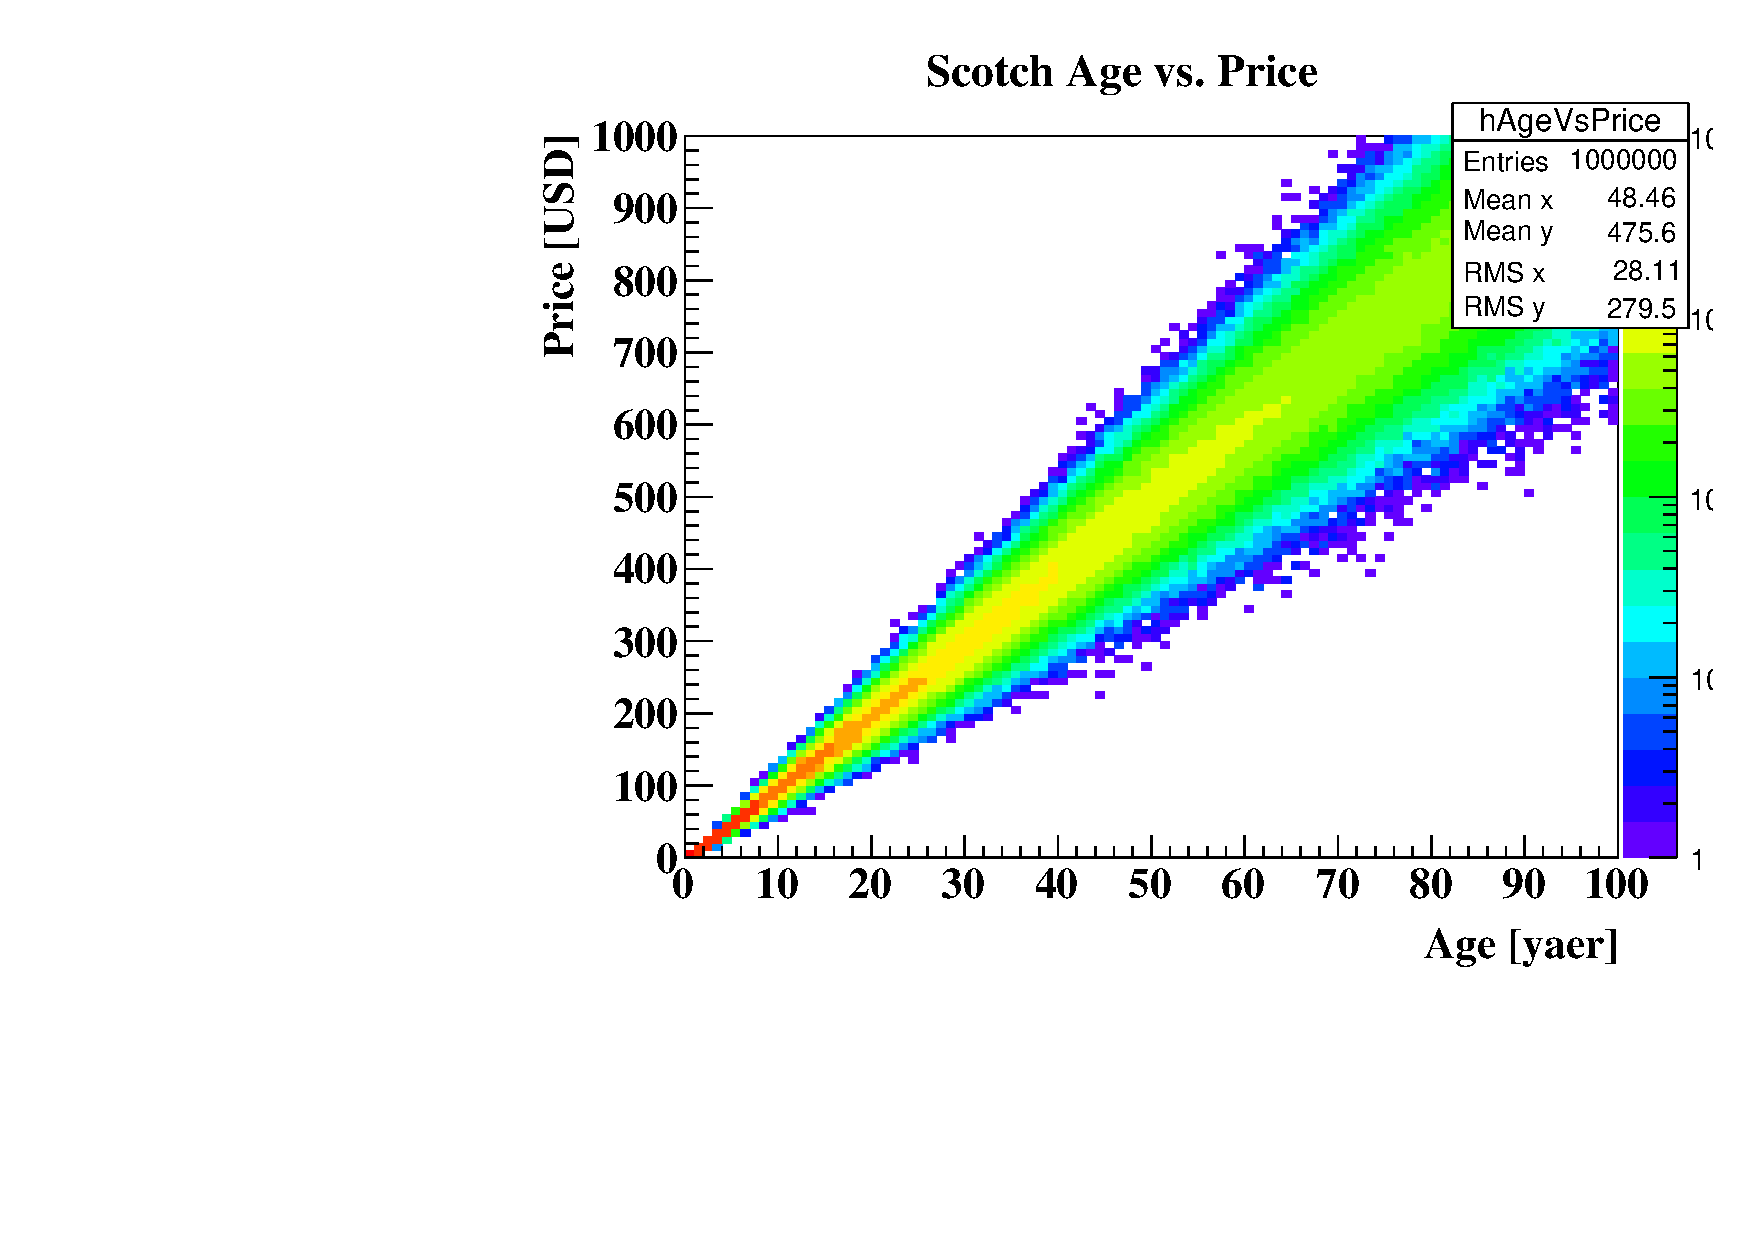
\includegraphics[width=12cm]{./img/ScotchAgeVsPrice.pdf}
\caption{ 
Drawing the age vs. price distribution of {\ttfamily example::Scotch} class from {\ttfamily TTree::Draw}.
}
\end{center}\end{figure}

An example script {\ttfamily mac/example.py} demonstrates how you can:
\begin{itemize}
\item Instantiate {\ttfamily example::Scotch} and save it in a \ROOT file
\item Create a {\ttfamily TTree} of {\ttfamily example::Scotch} for 1e6 entries and save
\item Read-in stored {\ttfamily TTree} and make a very simple access to the stored data product
\item Read-in stored {\ttfamily TTree} and call {\ttfamily TTree::Draw} on the stored data product
\end{itemize}

Note that storing multiple variables into a separate branch of {\ttfamily TTree} (i.e. Ntuple approach)
is much more tedious than storing a class instance as demonstrated in {\ttfamily Scotch::ShipScotch}
function. There, you can find a single line to create a {\ttfamily TTree} branch:
\begin{lstlisting}
tree.Branch("scotch",&data);
\end{lstlisting}
where ``data'' is a {\ttfamily example::Scotch} instance.
With this single line call, all variables in {\ttfamily example::Scotch} instance is stored
with a proper type, and will be readout correctly.

Another myth often people have is that it is very hard to access this object information from
{\ttfamily TTree}. As you can see in the {\ttfamily example.py}, this is completely irrelevant:
you can access the object directly via branch name. A single line in {\ttfamily Python} from
the script is shown below:
\begin{lstlisting}
ch.scotch.Speak()
\end{lstlisting}
which accesses the stored object and calling the class member function {\ttfamily example::Beer::Speak()}.

\subsection{Package Dependency}
The package {\ttfamily Example/Dependent} is prepared to demonstrate how one can make an inter-package 
dependency. In particular, this package depends on {\ttfamily Example/Function} package. Make sure
you have finished building {\ttfamily Example/Function} before building this package.

As you can see in {\ttfamily Stout.h}, the \CPP class {\ttfamily example::Stout} inherits from
{\ttfamily example::Beer}. In order to avoid re-compilation of {\ttfamily example::Beer} class,
we take a usual approach of just {\it linking} the libraries together. Take a look at 
{\ttfamily GNUmakefile}, in particular the following lines:
\begin{lstlisting}
...
INCFLAGS += -I$(LARLITE_USERDEVDIR)/Example
...
LDFLAGS += -L$(LARLITE_LIBDIR) -lExample_Function
\end{lstlisting}
As advertised in the previous section, you must include the path to find {\ttfamily Beer.h} (which
is called from {\ttfamily Stout.h} via {\ttfamily \#include ``Beer.h''}) in {\ttfamily INCFLAGS}, and
both a path and name of a library that contains {\ttfamily example::Beer} class definition in
{\ttfamily LDFLAGS}. 

An example script {\ttfamily mac/example.py} demonstrates an instantiation of {\ttfamily example::Stout}
class and also a call to its base class function {\ttfamily example::Beer::Speak()}.

\subsection{\python in \CPP}
Finally, some users are interested in developing \CPP code to directly operate on \python objects.
An example {\ttfamily Example/PyExample} is prepared to give a tip on how one can write a \CPP
API for \python. This is much better documented as a part of \python documentation:
\begin{center}
{\color{blue}\url{https://docs.python.org/2/c-api/}}
\end{center}

Using a native \python \CPP API is not very easy nor straight forward. Hence in this example,
again, we use \PyROOT binding that makes our life much easier. In short, a difference of two
methods is that you do not have to write your own binding, which is an extra code that has nothing
to do with your algorithm. Finally, that being said, there are other bindings available out there
such as {\ttfamily Cython} (... and \PyROOT uses one of them underneath anyways).

\subsubsection{External Dependnecy}
First of all, you will be using native \python classes, hence you will depend on \python.
Accordingly you have to modify {\ttfamily GNUmakefile}, in particular {\ttfamily INCFLAGS} and
{\ttfamily LDFLAGS}. Notice following 2 lines in {\ttfamily GNUmakefile}:
\begin{lstlisting}
...
INCFLAGS += $(shell python-config --includes)
...
LDFLAGS += $(shell python-config --ldflags)
\end{lstlisting}
each specifying an extra path to find a \python header file and libraries.

\subsubsection{Hiding \python Header From \CINT}
\python header file is called {\ttfamily Python.h}, and is not parse-able via \ROOT \CINT
compiler. So you have to hide it from \CINT dictionary generation step. This can be seen
in {\ttfamily PyExample.h} header file:
\begin{lstlisting}
...
#ifndef __CINT__
// You have to hide native Python header include from CINT                                                                                                                                                  
#include "Python.h"
#endif
...
\end{lstlisting}

You also need to provide two magic lines to forward declare types:
\begin{lstlisting}
...
struct _object;
typedef _object PyObject;
...
\end{lstlisting}
which is for \python generic object pointers to be used (this is a part of \python \CPP API).

\subsubsection{{\ttfamily example::PyExample::Convert}}
The example class {\ttfamily example::PyExample} has an example function to create a
\python list from a \CPP {\ttfamily std::vector<std::string>} object. You can look at the
source code as to how one can do this very simple operation, and take a look at \python
documentation for doing more elaborate operations.

Running {\ttfamily mac/example.py} should show you how this function works.
Obviously you may want to expand the code to work with more advanced \python objects
such as {\ttfamily numpy} array, {\ttfamily matplotlib} axis, and such. The author
does not have much experience to extend too far, but is happy to discuss if you need a help.

\subsection{Documenting Code Using {\ttfamily Doxygen}}
Though this is not everyone's favorite choice, {\ttfamily doxygen} is a popular method to
provide an in-line documentation in the source code. It works pretty nicely with \CPP, and
somewhat at acceptable level with \python. It is the recommended choice for LArSoft to provide
a minimal documentation.

LArLite repositories comes with a doxygen script. You can try generating a documentation
in {\ttfamily Example} directory by typing:
\begin{lstlisting}
  > make doxygen
\end{lstlisting}
({\bf you need doxygen installed in your system!}).

\begin{figure}[htb]\begin{center}
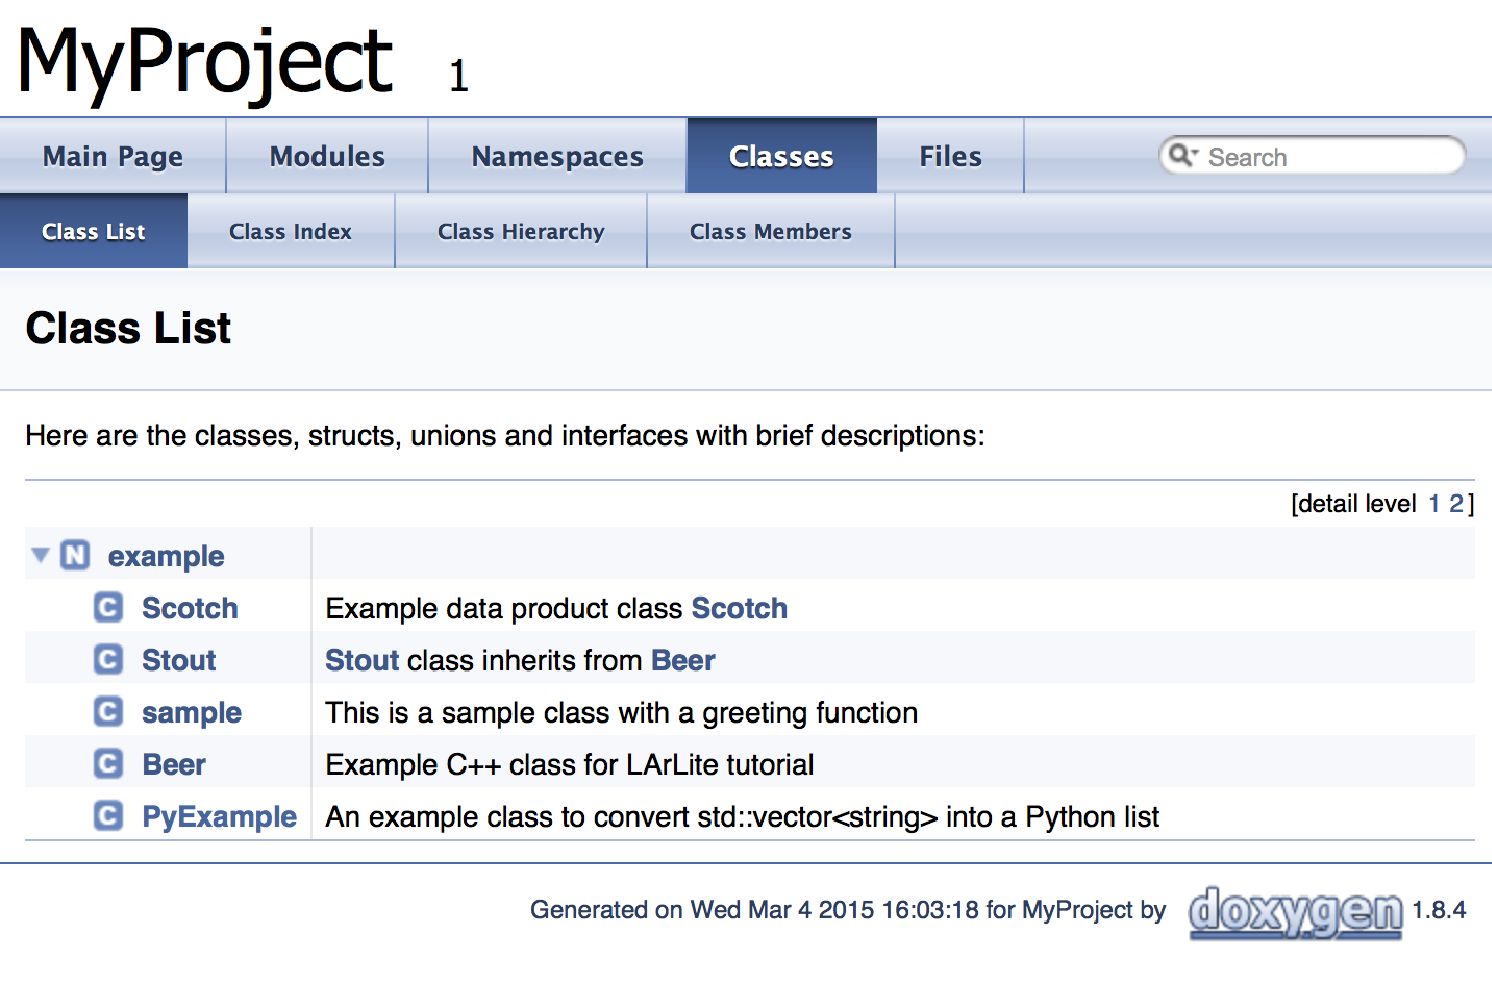
\includegraphics[width=12cm]{./img/doxygen.pdf}
\caption{ 
Doxygen web page generated by ``{\ttfamily make doxygen}'' command for {\ttfamily Example} repository.
}
\end{center}\end{figure}

After successfully running the above command, you should find a chain of HTML files 
to browse through (no internet needed). This way you can also check your doxygen comment
format (whether this is correct or not) before you commit the code. You can look at the
generated documentation using a command like below:
\begin{lstlisting}
  > firefox -a doc/dOxygenMyProject/html/index.html 
\end{lstlisting}
on {\ttfamily Linux} or
\begin{lstlisting}
  > open doc/dOxygenMyProject/html/index.html 
\end{lstlisting}
on {\ttfamily OSX}. The figure shows a generated documentation webpage on the author's laptop.

To understand {\ttfamily doxygen} comment style, refer to their web documentation:
\begin{center}
{\color{blue}\url{http://www.stack.nl/~dimitri/doxygen/manual/docblocks.html}}
\end{center}



%
%%% Appendix
%
%\appendix
%\appendixpage

% Bibliography
\bibliographystyle{unsrt}

\bibliography{LArLight}


\end{document}
